\documentclass[twoside,openright,10pt]{report}
%\documentclass[openright,10pt]{report}

% Package useful for debuging
%\usepackage{showlabels}

\usepackage{epsfig, supertabular, makeidx}
\usepackage{amsmath, amssymb}

% Package to add Bibliography and Index to TOC
% but not the TOC itself :-)
\usepackage[nottoc]{tocbibind}

\usepackage{hangcaption}
\usepackage{subfigure}

\usepackage{color}

% Packages needed for the cover page
\usepackage{calc, epsfig, chngpage}
\input{pstricks}\input{pst-node}\input{llnlCoverPage}

% Package useful for debuging
\usepackage{showlabels}

%----- Define some colors
\definecolor{gray}{rgb}{0.5,0.5,0.5} 

%----- Page formatting
\setlength{\oddsidemargin}{0in}
\setlength{\evensidemargin}{0in}
\setlength{\textwidth}{6.5in}
\setlength{\textheight}{8.5in}

%----- SUNDIALS MODULES
\newcommand{\sundials}{{\normalfont\scshape sundials}}
\newcommand{\nvector}{{\normalfont\scshape nvector}}
\newcommand{\nvecp}{{\normalfont\scshape nvector\_parallel}}
\newcommand{\nvecs}{{\normalfont\scshape nvector\_serial}}
\newcommand{\cvode}{{\normalfont\scshape cvode}}
\newcommand{\pvode}{{\normalfont\scshape pvode}}
\newcommand{\cvodes}{{\normalfont\scshape cvodes}}
\newcommand{\ida}{{\normalfont\scshape ida}}
\newcommand{\idas}{{\normalfont\scshape idas}}
\newcommand{\kinsol}{{\normalfont\scshape kinsol}}
\newcommand{\kinsols}{{\normalfont\scshape kinsols}}

%----- OTHER PACKAGES
\newcommand{\vode}{{\normalfont\scshape vode}}
\newcommand{\vodpk}{{\normalfont\scshape vodpk}}
\newcommand{\lsode}{{\normalfont\scshape lsode}}

%----- CVODES COMPONENTS
\newcommand{\cvdense}{{\normalfont\scshape cvdense}}
\newcommand{\cvband}{{\normalfont\scshape cvband}}
\newcommand{\cvdiag}{{\normalfont\scshape cvdiag}}
\newcommand{\cvspgmr}{{\normalfont\scshape cvspgmr}}
\newcommand{\cvbandpre}{{\normalfont\scshape cvbandpre}}
\newcommand{\cvbbdpre}{{\normalfont\scshape cvbbdpre}}
\newcommand{\stald}{{\normalfont\scshape stald}}

%----- SHARED COMPONENTS
\newcommand{\sundialsmath}{{\normalfont\scshape sundialsmath}}
\newcommand{\dense}{{\normalfont\scshape dense}}
\newcommand{\band}{{\normalfont\scshape band}}
\newcommand{\spgmr}{{\normalfont\scshape spgmr}}

%----- C and Fortran languages
\newcommand{\C}{{\sc C}}
\newcommand{\CPP}{{\sc C++}}
\newcommand{\F}{{\sc Fortran}}

%------ Serial or Parallel
\newcommand{\p}{[{\bf P}]}
\newcommand{\s}{[{\bf S}]}

%------ Appendix in text
\newcommand{\A}{App. }

%------ Index entries
\newcommand{\ID}[1]{{\tt #1}{\index{#1@\texttt{#1}|textbf}}}
\newcommand{\Id}[1]{{\tt #1}{\index{#1@\texttt{#1}}}}
\newcommand{\id}[1]{{\tt #1}}

%------ Cross reference to the user guide
\newcommand{\ugref}[1]{\ref{#1} in the user guide}

%%----- Shortcuts for math formulas
\newcommand{\mb}[1]{{\mbox{\scriptsize #1}}}
\newcommand{\dfdy}{\frac{\partial f}{\partial y}}
\newcommand{\dfdyI}{\partial f / \partial y}
\newcommand{\dfdpi}{\frac{\partial f}{\partial p_i}}
\newcommand{\dfdpiI}{\partial f / \partial p_i}
\newcommand{\rhomax}{\rho_{\max}}

%%--------------------------------
\newcommand{\frontug}
{
  \maketitle

  %% Leave an empty page
  \newpage\thispagestyle{empty}
  \vspace*{1.0in}
  
  %% Start roman numbering
  \pagestyle{plain}\pagenumbering{roman}
  \tableofcontents
  \listoftables
  \listoffigures
  
  \newpage\thispagestyle{empty}
  \vspace*{1.0in}
  
  %% Move to new page and start arabic numbering
  \newpage\pagestyle{plain}\pagenumbering{arabic}
}

%%--------------------------------
\newcommand{\frontex}
{
  \maketitle

  %% Leave an empty page
  \newpage\thispagestyle{empty}
  \vspace*{1.0in}
  
  %% Start roman numbering
  \pagestyle{plain}\pagenumbering{roman}
  \tableofcontents
  
  %% Move to new page and start arabic numbering
  \newpage\pagestyle{plain}\pagenumbering{arabic}
}

%%---------------------------------
%% Steps used in scheleton programs
%%---------------------------------
\newcounter{Stepsctr}
\newenvironment{Steps}
{\stepcounter{Stepsctr}
  \begin{list}{\arabic{Stepsctr}. }{
      \usecounter{Stepsctr}
      \setlength{\parsep}{0.5em}
      \setlength{\labelsep}{0em}
      \settowidth{\labelwidth}{99. }
      \setlength{\leftmargin}{\labelwidth+\labelsep}}}
  {\end{list}}
%%-----------------------------------------------------
%% Underlying list environemnt for function definitions
%%-----------------------------------------------------
\newenvironment{Ventry}[1][\quad]
{\begin{list}{}{
      \setlength{\rightmargin}{0em}
      \setlength{\topsep}{0.15in}
      \setlength{\itemsep}{0em}
      \renewcommand{\makelabel}[1]{##1\hfill}
      \settowidth{\labelwidth}{#1}
      \setlength{\leftmargin}{\labelwidth+\labelsep}}}
  {\end{list}}
%%----------------------------------
%% List of function arguments
%%---------------------------------
\newenvironment{args}[1][\quad]
{\begin{list}{}{
      \setlength{\rightmargin}{0em}
      \setlength{\topsep}{0em}
      \setlength{\itemsep}{0em}
      \renewcommand{\makelabel}[1]{\id{##1}\hfill}
      \settowidth{\labelwidth}{\id{#1}}
      \setlength{\leftmargin}{\labelwidth+\labelsep}}}
  {\end{list}}
%%---------------------------------
%% User-callable function
%%---------------------------------
\newcommand{\ucfunction}[6]{
  \begin{Ventry}[Return value]
  \item[\fbox{\id{#1}}]{}
  \item[Call]{\id{#2}}
  \item[Description]{#3}
  \item[Arguments]{#4}
  \item[Return value]{#5}
  \addNotes{#6}
  \end{Ventry}
}
%%---------------------------------
%% User-supplied function
%%---------------------------------
\newcommand{\usfunction}[6]{
  \begin{Ventry}[Return value]
  \item[\fbox{\id{#1}}]{}
  \item[Definition]{\id{\begin{tabular}[t]{@{}r@{}l@{}}#2\end{tabular}}}
  \item[Purpose]{#3}
  \item[Arguments]{#4}
  \item[Return value]{#5}
  \addNotes{#6}
  \end{Ventry}
}
%%---------------------------------
\makeatletter
\long\def\addNotes#1{\def\@tempa{#1}\ifx\@tempa\empty\else\item[Notes]{#1}\fi}
\makeatother

%===============================================================

\title{User Documentation for {\ida} {\idarelease}}
\author{
  Radu Serban and Cosmin Petra\\
  {\em Center for Applied Scientific Computing} \\
  {\em Lawrence Livermore National Laboratory}
}
\date{
  \today 
  \vfill 
  {\centerline{\psfig{figure=doc_logo.eps,width=0.5\textwidth}}}
  \vfill \idaucrlug
}

%===============================================================

\makeindex

%===============================================================

\begin{document}

\frontug
\renewcommand{\chaptermark}[1]{\markboth{#1}{}}
\renewcommand{\sectionmark}[1]{\markright{\thesection\ #1}}

%===============================================================
% Introduction
%===================================================================================
\chapter{Introduction}\label{s:intro}
%===================================================================================

{\idas} is part of a software family called {\sundials}: 
SUite of Nonlinear and DIfferential/ALgebraic equation Solvers~\cite{HBGLSSW:05}. 
This suite consists of {\cvode}, {\kinsol}, and {\ida}, and variants of these
with sensitivity analysis capabilities, {\cvodes} and {\idas}.

{\idas} is a general purpose solver for the initial value problem (IVP) for
systems of differential-algebraic equations (DAEs).  The name IDAS
stands for Implicit Differential-Algebraic solver with Sensitivity capabilities.
{\idas} is an extension of the {\ida} solver within {\sundials}, itself 
based on {\daspk}~\cite{BHP:94,BHP:98}; however, like all {\sundials} solvers,
{\idas} is written in ANSI-standard C rather than {\F}77.  
Its most notable features are that, 
(1) in the solution of the underlying nonlinear system at each time step, it 
offers a choice of Newton/direct methods and a choice of Inexact Newton/Krylov
(iterative) methods;
(2) it is written in a {\em data-independent} manner in that it acts
on generic vectors without any assumptions on the underlying organization
of the data; and
(3) it provides a flexible, extensible framework for sensitivity analysis,
using either {\em forward} or {\em adjoint} methods.
Thus {\idas} shares significant modules previously written within CASC
at LLNL to support the ordinary differential equation (ODE) solvers
{\cvode}~\cite{cvode_ug,CoHi:96} and {\pvode}~\cite{ByHi:98,ByHi:99},
the DAE solver {\ida}~\cite{ida_ug} on which {\idas} is based, the
sensitivity-enabled ODE solver {\cvodes}~\cite{cvodes_ug,SeHi:05}, and
also the nonlinear system solver {\kinsol}~\cite{kinsol_ug}.

The Newton/Krylov methods in {\idas} are:
the GMRES (Generalized Minimal RESidual)~\cite{SaSc:86},
Bi-CGStab (Bi-Conjugate Gradient Stabilized)~\cite{Van:92}, and
TFQMR (Transpose-Free Quasi-Minimal Residual) linear iterative 
methods~\cite{Fre:93}.  As Krylov methods, these require almost no 
matrix storage for solving the Newton equations as compared to direct
methods. However, the algorithms allow for a user-supplied preconditioner
matrix, and for most problems preconditioning is essential for an
efficient solution.

For very large DAE systems, the Krylov methods are preferable over
direct linear solver methods, and are often the only feasible choice.
Among the three Krylov methods in {\idas}, we recommend GMRES as the
best overall choice.  However, users are encouraged to compare all
three, especially if encountering convergence failures with GMRES.
Bi-CGFStab and TFQMR have an advantage in storage requirements, in
that the number of workspace vectors they require is fixed, while that
number for GMRES depends on the desired Krylov subspace size.

\index{IDAS@{\idas}!relationship to {\ida}|(}
{\idas} is written with a functionality that is a superset of that
of {\ida}. Sensitivity analysis capabilities, both
forward and adjoint, have been added to the main integrator. Enabling
forward sensitivity computations in {\idas} will result in the
code integrating the so-called {\em sensitivity equations}
simultaneously with the original IVP, yielding both the solution and
its sensitivity with respect to parameters in the model. Adjoint
sensitivity analysis, most useful when the gradients of relatively few
functionals of the solution with respect to many parameters are
sought, involves integration of the original IVP forward in time
followed by the integration of the so-called {\em adjoint equations}
backward in time. {\idas} provides the infrastructure needed to
integrate any final-condition ODE dependent on the solution of the
original IVP (in particular the adjoint system).
\index{IDAS@{\idas}!relationship to {\ida}|)}

\index{IDAS@{\idas}!motivation for writing in C|(}
There are several motivations for choosing the {\C} language for {\idas}.
First, a general movement away from {\F} and toward {\C} in scientific
computing is apparent.  Second, the pointer, structure, and dynamic
memory allocation features in {\C} are extremely useful in software of
this complexity, with the great variety of method options offered.
Finally, we prefer {\C} over {\CPP} for {\idas} because of the wider
availability of {\C} compilers, the potentially greater efficiency of {\C},
and the greater ease of interfacing the solver to applications written
in extended {\F}.
\index{IDAS@{\idas}!motivation for writing in C|)}


\section{Changes from previous versions}

\subsection*{Changes in v1.2.0}

Two major additions were made to the linear system solvers that are
available for use with the {\idas} solver.  First, in the serial case,
an interface to the sparse direct solver KLU was added.
Second, an interface to SuperLU\_MT, the multi-threaded version of
SuperLU, was added as a thread-parallel sparse direct solver option,
to be used with the serial version of the NVECTOR module.
As part of these additions, a sparse matrix (CSC format) structure 
was added to {\idas}.

Otherwise, only relatively minor modifications were made to {\idas}:

In \id{IDARootfind}, a minor bug was corrected, where the input
array \id{rootdir} was ignored, and a line was added to break out of
root-search loop if the initial interval size is below the tolerance
\id{ttol}.

In \id{IDALapackBand}, the line \id{smu = MIN(N-1,mu+ml)} was changed to
\id{smu = mu + ml} to correct an illegal input error for \id{DGBTRF/DGBTRS}.

An option was added in the case of Adjoint Sensitivity Analysis with
dense or banded Jacobian:  With a call to \id{IDADlsSetDenseJacFnBS} or
\id{IDADlsSetBandJacFnBS}, the user can specify a user-supplied Jacobian
function of type \id{IDADls***JacFnBS}, for the case where the backward
problem depends on the forward sensitivities.

In the User Guide, a paragraph was added in Section 6.2.1 on
\id{IDAAdjReInit}, and a paragraph was added in Section 6.2.9 on
\id{IDAGetAdjY}.

Two new {\nvector} modules have been added for parallel computing
environments --- one for openMP, denoted \id{NVECTOR\_OPENMP},
and one for Pthreads, denoted \id{NVECTOR\_PTHREADS}.

With this version of {\sundials}, support and documentation of the
Autotools mode of installation is being dropped, in favor of the
CMake mode, which is considered more widely portable.

\subsection*{Changes in v1.1.0}

One significant design change was made with this release: The problem
size and its relatives, bandwidth parameters, related internal indices,
pivot arrays, and the optional output \id{lsflag} have all been
changed from type \id{int} to type \id{long int}, except for the
problem size and bandwidths in user calls to routines specifying
BLAS/LAPACK routines for the dense/band linear solvers.  The function
\id{NewIntArray} is replaced by a pair \id{NewIntArray}/\id{NewLintArray},
for \id{int} and \id{long int} arrays, respectively.  In a minor
change to the user interface, the type of the index \id{which} in
IDAS was changed from \id{long int} to \id{int}.

Errors in the logic for the integration of backward problems were
identified and fixed.

A large number of minor errors have been fixed.  Among these are the following:
A missing vector pointer setting was added in \id{IDASensLineSrch}.
In \id{IDACompleteStep}, conditionals around lines loading a new column of three
auxiliary divided difference arrays, for a possible order increase, were fixed.
After the solver memory is created, it is set to zero before being filled.
In each linear solver interface function, the linear solver memory is
freed on an error return, and the \id{**Free} function now includes a
line setting to NULL the main memory pointer to the linear solver memory.
A memory leak was fixed in two of the \id{IDASp***Free} functions.
In the rootfinding functions \id{IDARcheck1}/\id{IDARcheck2}, when an exact
zero is found, the array \id{glo} of $g$ values at the left endpoint is
adjusted, instead of shifting the $t$ location \id{tlo} slightly.
In the installation files, we modified the treatment of the macro
SUNDIALS\_USE\_GENERIC\_MATH, so that the parameter GENERIC\_MATH\_LIB is
either defined (with no value) or not defined.


\section{Reading this User Guide}\label{ss:reading}

The structure of this document is as follows:
\begin{itemize}
\item
  In Chapter \ref{s:math}, we give short descriptions of the numerical 
  methods implemented by {\idas} for the solution of initial value problems
  for systems of DAEs, continue with short descriptions of preconditioning
  (\S\ref{s:preconditioning}) and rootfinding (\S\ref{s:rootfinding}), and
  then give an overview of the mathematical aspects of sensitivity analysis,
  both forward (\S\ref{ss:fwd_sensi}) and adjoint (\S\ref{ss:adj_sensi}).
\item
  The following chapter describes the structure of the {\sundials} suite
  of solvers (\S\ref{ss:sun_org}) and the software organization of the {\idas}
  solver (\S\ref{ss:idas_org}). 
\item
  Chapter \ref{s:simulation} is the main usage document for {\idas}
  for simulation applications.  It includes a complete description of
  the user interface for the integration of DAE initial value problems.
  Readers that are not interested in using {\idas} for sensitivity
  analysis can then skip the next two chapters.
\item
  Chapter \ref{s:forward} describes the usage of {\idas} for forward
  sensitivity analysis as an extension of its IVP integration
  capabilities.  We begin with a skeleton of the user main program,
  with emphasis on the steps that are required in addition to those
  already described in Chapter \ref{s:simulation}.  Following that we
  provide detailed descriptions of the user-callable interface
  routines specific to forward sensitivity analysis and of the
  additonal optional user-defined routines.
\item
  Chapter \ref{s:adjoint} describes the usage of {\idas} for adjoint
  sensitivity analysis. We begin by describing the {\idas} checkpointing 
  implementation for interpolation of the original IVP solution during
  integration of the adjoint system backward in time, and with 
  an overview of a user's main program. Following that we provide complete
  descriptions of the user-callable interface routines for adjoint sensitivity
  analysis as well as descriptions of the required additional user-defined routines.
\item
  Chapter \ref{s:nvector} gives a brief overview of the generic
  {\nvector} module shared amongst the various components of
  {\sundials}, as well as details on the two {\nvector}
  implementations provided with {\sundials}: a serial implementation
  (\S\ref{ss:nvec_ser}) and a parallel implementation based on
  {\mpi}\index{MPI} (\S\ref{ss:nvec_par}).
\item
  Chapter \ref{s:new_linsolv} describes the specifications of linear
  solver modules as supplied by the user.
\item
  Chapter \ref{s:gen_linsolv} describes in detail the generic linear solvers shared 
  by all {\sundials} solvers.
\item
  Finally, in the appendices, we provide detailed instructions for the installation
  of {\idas}, within the structure of {\sundials} (Appendix \ref{c:install}), as
  well as a list of all the constants used for input to and output from {\idas}
  functions
  (Appendix \ref{c:constants}).
\end{itemize}

The reader should be aware of the following notational conventions
in this user guide:  program listings and identifiers (such as \id{IDAInit}) 
within textual explanations appear in typewriter type style; 
fields in {\C} structures (such as {\em content}) appear in italics;
and packages or modules, such as {\idadense}, are written in all capitals. 
Usage and installation instructions that constitute important warnings
are marked with a triangular symbol {\warn} in the margin.

\clearemptydoublepage
%===============================================================
% SUNDIALS installation procedure
\chapter{IDAS Installation Procedure}\label{s:install}

The installation of {\idas} is accomplished by installing the
{\sundials} suite as a whole, according to the instructions that
follow.   The same procedure applies whether or not the downloaded
file contains solvers other than {\idas}.

The {\sundials} suite (or individual solvers) are distributed as compressed archives
(\id{.tgz}). The name of the distribution archive is of the form {\em solver}\id{-x.y.z.tgz},
where {\em solver} is one of: \id{sundials}, \id{cvode}, \id{cvodes}, \id{ida}, or \id{kinsol},
and \id{x.y.z} represents the version number (of the {\sundials} suite or of the individual solver).

To begin the installation, first uncompress and expand the sources, by issuing
\begin{verbatim}
   % tar xzf solver-x.y.z.tgz
\end{verbatim}
This will extract source files under a directory {\em solver}\id{-x.y.z}.

The installation procedure outlined below will work on commodity {\linux}/{\unix} 
systems without modification. However, users are still encouraged to carefully read 
the entire chapter before attempting to install the {\sundials} suite, in case
non-default choices are desired for compilers, compilation options, or the like.
In lieu of reading the option list below, the user may invoke the configuration
script with the help flag to view a complete listing of available options, which
may be done by issuing 
\begin{verbatim}
   % ./configure --help 
\end{verbatim}
from within the directory created above.

In the remainder of this chapter, we make the following distinctions:
\begin{itemize}

\item {\em srcdir} 

  is the directory {\em solver}\id{-x.y.z} created above; i.e., the 
  directory containing the {\sundials} sources.

\item {\em builddir}

  is the directory under which {\sundials} is built; i.e., the directory
  from within which the \id{configure} command is issued. Usually, this is the same as
  {\em srcdir}.

\item {\em instdir}

  is the directory under which the {\sundials} exported header files
  and libraries will be installed. Typically, header files are exported under a directory
  {\em instdir}\id{/include} while libraries are installed under {\em instdir}\id{/lib},
  with {\em instdir} specified with the \id{--prefix} flag to \id{configure}. 
  See \S\ref{ss:configuration_options} for more details on the installation directories, 
  including the special cases of the {\sundials} examples and the {\sundialsTB} toolbox.

\end{itemize}
{\noindent}{\warn}{\em Note}: The installation directory {\em instdir} should {\em not} be the same as
the source directory {\em srcdir}.

\vspace{0.2in}
{\noindent}The installation steps for {\sundials} can be as simple as 
\begin{verbatim}
   % tar xzf solver-x.y.z.tgz
   % cd solver-x.y.z
   % ./configure
   % make
   % make install
\end{verbatim}
in which case the {\sundials} header files and libraries are installed under \id{/usr/local/include}
and \id{/usr/local/lib}, respectively. Note that, by default, neither the example programs nor the 
{\sundialsTB} toolbox are built and installed.

If disk space is a priority, then to delete all temporary files created by building {\sundials}, issue
\begin{verbatim}
   % make clean
\end{verbatim}

To prepare the {\sundials} distribution for a new install (using, for example, different options and/or
installation destinations), issue
\begin{verbatim}
   % make distclean
\end{verbatim}

%===============================================================================

\section{Configuration options}\label{ss:configuration_options}

The installation procedure given above will generally work without modification;
however, if the system includes multiple {\mpi} implementations, then certain
configure script-related options may be used to indicate which {\mpi}
implementation should be used. Also, if the user wants to use non-default
language compilers, then, again, the necessary shell environment variables must
be appropriately redefined.
%%
The remainder of this section provides explanations of available configure script
options.


\subsection*{General options}

%%
%% General options
%%

\begin{config}
  
\item \id{--prefix=PREFIX}
  
  Location for architecture-independent files.
  
  Default: \id{PREFIX=}{/usr/local}
  
\item \id{--exec-prefix=EPREFIX}

  Location for architecture-dependent files.
  
  Default: \id{EPREFIX=}{/usr/local}

\item \id{--includedir=DIR}
  
  Alternate location for installation of header files.
  
  Default: \id{DIR=PREFIX/include}
  
\item \id{--libdir=DIR}
  
  Alternate location for installation of libraries.
  
  Default: \id{DIR=EPREFIX/lib}

\item \id{--disable-}{\em solver}

  Although each existing solver module is built by default, support for a
  given solver can be explicitly disabled using this option. 
  The valid values for {\em solver} are: \id{cvode}, \id{cvodes}, 
  \id{ida}, and \id{kinsol}.

\item \id{--enable-examples}
  
  Available example programs are {\em not} built by default. Use this option
  to enable compilation of all pertinent example programs. Upon completion of 
  the \id{make} command, the example executables will be created under solver-specific
  subdirectories of {\em builddir}\id{/examples}:
  \begin{config}
  \item {\em builddir}\id{/examples/}{\em solver}\id{/serial} : serial {\C} examples
  \item {\em builddir}\id{/examples/}{\em solver}\id{/parallel} : parallel {\C} examples
  \item {\em builddir}\id{/examples/}{\em solver}\id{/fcmix\_serial} : serial {\F} examples
  \item {\em builddir}\id{/examples/}{\em solver}\id{/fcmix\_parallel} : parallel {\F} examples
  \end{config}  
  {\em Note}: Some of these subdirectories may not exist depending upon the
  solver and/or the configuration options given.

\item \id{--with-examples-instdir=EXINSTDIR}

  Alternate location for example executables and sample output files (valid only if
  examples are enabled). Note that installtion of example files can be completely disabled
  by issuing \id{EXINSTDIR=no} (in case building the examples is desired only as a test of
  the {\sundials} libraries).

  Default: \id{DIR=EPREFIX/examples}

\item \id{--with-cppflags=ARG}

  Specify additional {\C} preprocessor flags 
  (e.g., \id{ARG=-I<include\_dir>} if necessary header files are located in
   nonstandard locations).

\item \id{--with-cflags=ARG}

  Specify additional {\C} compilation flags.

\item \id{--with-ldflags=ARG}

  Specify additional linker flags (e.g., \id{ARG=-L<lib\_dir>} if
  required libraries are located in nonstandard locations).

\item \id{--with-libs=ARG}

  Specify additional libraries to be used (e.g., \id{ARG=-l<foo>} to
  link with the library named \id{libfoo.a} or \id{libfoo.so}).

\item \id{--with-precision=ARG}

  By default, {\sundials} will define a real number (internally referred to as
  \id{realtype}) to be a double-precision floating-point numeric data type
  (\id{double} {\C}-type); however, this option may be used to build {\sundials}
  with \id{realtype} alternatively defined as a single-precision floating-point
  numeric data type (\id{float} {\C}-type) if \id{ARG=single}, or as a
  \id{long double} {\C}-type if \\ \id{ARG=extended}.

  Default: \id{ARG=double}

  {\warn}Users should {\em not} build {\sundials} with support for
  single-precision floating-point arithmetic on 32- or 64-bit systems.
  This will almost certainly result in unreliable numerical solutions.
  The configuration option \id{--with-precision=single} is intended for
  systems on which single-precision arithmetic involves at least 14 decimal
  digits.

\end{config}

%%
%% Fortran support
%%

\subsection*{Options for Fortran support}

\begin{config}

\item \id{--disable-f77}

  Using this option will disable all {\F} support. The {\fcvode},
  {\fkinsol}, {\fida}, and {\fnvector} modules will not be built,
  regardless of availability.

\item \id{--with-fflags=ARG}

  Specify additional {\F} compilation flags.

\end{config}

\noindent The configuration script will attempt to automatically determine the
function name mangling scheme required by the specified {\F} compiler, but the
following two options may be used to override the default behavior.

\begin{config}

\item \id{--with-f77underscore=ARG}

  This option pertains to the {\fcvode}, {\fkinsol}, {\fida}, and {\fnvector}
  {\F}-{\C} interface modules and is used to specify the number of underscores to
  append to function names so {\F} routines can properly link with the associated
  {\sundials} libraries. Valid values for \id{ARG} are: \id{none}, \id{one}
  and \id{two}.

  Default: \id{ARG=one}

\item \id{--with-f77case=ARG}

  Use this option to specify whether the external names of the {\fcvode},
  {\fkinsol}, {\fida}, and {\fnvector} {\F}-{\C} interface functions should be
  lowercase or uppercase so {\F} routines can properly link with the associated
  {\sundials} libraries. Valid values for \id{ARG} are: \id{lower} and \id{upper}.

  Default: \id{ARG=lower}

\end{config}


%%
%% Parallel options
%%

\subsection*{Options for MPI support}

\noindent The following configuration options are only applicable to the parallel
{\sundials} packages:

\begin{config}
  
\item \id{--disable-mpi}

  Using this option will completely disable {\mpi} support.

\item \id{--with-mpicc=ARG}
\item \id{--with-mpif77=ARG}

  By default, the configuration utility script will use the {\mpi} compiler
  scripts named \id{mpicc} and \id{mpif77} to compile the parallelized
  {\sundials} subroutines; however, for reasons of compatibility, different
  executable names may be specified via the above options. Also, \id{ARG=no}
  can be used to disable the use of {\mpi} compiler scripts, thus causing
  the serial {\C} and {\F} compilers to be used to compile the parallelized
  {\sundials} functions and examples.

\item \id{--with-mpi-root=MPIDIR}

  This option may be used to specify which {\mpi} implementation should be used.
  The {\sundials} configuration script will automatically check under the
  subdirectories \id{MPIDIR/include} and \id{MPIDIR/lib} for the necessary
  header files and libraries. The subdirectory \id{MPIDIR/bin} will also be
  searched for the {\C} and {\F} {\mpi} compiler scripts, unless the user uses
  \id{--with-mpicc=no} or \id{--with-mpif77=no}.

\item \id{--with-mpi-incdir=INCDIR}
\item \id{--with-mpi-libdir=LIBDIR}
\item \id{--with-mpi-libs=LIBS}

  These options may be used if the user would prefer not to use a preexisting
  {\mpi} compiler script, but instead would rather use a serial complier and
  provide the flags necessary to compile the {\mpi}-aware subroutines in
  {\sundials}.

  Often an {\mpi} implementation will have unique library names and so it may
  be necessary to specify the appropriate libraries to use (e.g.,
  \id{LIBS=-lmpich}).

  Default: \id{INCDIR=MPIDIR/include} and \id{LIBDIR=MPIDIR/lib}

\item \id{--with-mpi-flags=ARG}

  Specify additional {\mpi}-specific flags.

\end{config}


\subsection*{Options for library support}
%%
%% Shared or Static Libraries
%%

\noindent By default, only static libraries are built, but the following option
may be used to build shared libraries on supported platforms.

\begin{config}

\item \id{--enable-shared}

  Using this particular option will result in both static and shared versions of
  the available {\sundials} libraries being built if the system supports shared
  libraries. To build only shared libraries also specify \id{--disable-static}.

  {\em Note}: The {\fcvode}, {\fkinsol}, and {\fida} libraries can only be built as
  static libraries because they contain references to externally defined symbols,
  namely user-supplied {\F} subroutines.  Although the {\F} interfaces to the serial
  and parallel implementations of the supplied {\nvector} module do not contain any
  unresolvable external symbols, the libraries are still built as static libraries
  for the purpose of consistency.

\end{config}


\subsection*{Options for Matlab support}
%%
%% Compilation of sundialsTB mex files
%%

\noindent The following options are relevant only for configuring and building 
the {\sundialsTB} Matlab toolbox:

\begin{config}

\item \id{--enable-sundialsTB}

  The {\sundialsTB} Matlab toolbox is {\em not} built by default. Use this option
  to enable configuration and compilation of the \id{mex} files. Upon completion
  of the \id{make} command, the following \id{mex} files will be created:
  \begin{config}
    \item {\em builddir}\id{/sundialsTB/cvodes/cvm/cvm.}{\em{mexext}}
    \item {\em builddir}\id{/sundialsTB/idas/idm/idm.}{\em{mexext}}
    \item {\em builddir}\id{/sundialsTB/kinsol/kim/kim.}{\em{mexext}}
  \end{config}
  where {\em mexext} is the platform-specific extension of \id{mex} files.
  
\item \id{--with-sundialsTB-instdir=STBINSTDIR}

  Alternate location for the installed {\sundialsTB} toolbox (valid only if
  {\sundialsTB} is enabled). As for the example programs, installation of {\sundialsTB} can 
  be completely disabled by issuing \id{STBINSTDIR=no} (in case building the toolbox is desired 
  but its installtion will be done manually afterwards). Otherwise, all required {\sundialsTB} 
  files will be installed under the directory \id{STBINSTDIR/sundialsTB}.

  Default: \id{DIR=MATLAB/toolbox}  (see below for the definition of \id{MATLAB}).

\item \id{--with-matlab=MATLAB}

  This option can be used to specify the locatin of the Matlab installation. 
  If it is defined, the environment variable \id{MATLAB} will be used. Otherwise,
  the configure system will attempt to infer \id{MATLAB} from the location of
  the \id{matlab} executable.

\item \id{--with-mex=ARG}

  Specify the \id{mex} compiler to be used.

  Default: \id{ARG=MATLAB/bin/mex}

\item \id{--with-mexopts=ARG}

  Specify the \id{mex} options file to be used.

  Default: Standard Matlab \id{mex} options file.

\end{config}


\subsection*{Environment variables}

%%
%% Environment variables
%%

\noindent The following environment variables can be locally (re)defined for use 
during the configuration of {\sundials}. See the next section for
illustrations of these.

\begin{config}

\item \id{CC}

\item \id{F77}

  Since the configuration script uses the first {\C} and {\F} compilers found in
  the current executable search path, then each relevant shell variable (\id{CC}
  and \id{F77}) must be locally (re)defined in order to use a different compiler. 
  For example, to use \id{xcc} (executable name of chosen compiler) as the {\C}
  language compiler, use \id{CC=xcc} in the configure step.

\item \id{CFLAGS}

\item \id{FFLAGS}

  Use these environment variables to override the default {\C} and {\F}
  compilation flags.

\end{config}


%%===============================================================================


\section{Configuration examples}

The following examples are meant to help demonstrate proper usage of the configure options.


To build {\sundials} using the default C and Fortran compilers,
and default \id{mpicc} and \id{mpif77} parallel compilers, enable compilation of examples,
build the Matlab \id{mex} files for {\sundialsTB}, and install it under 
\id{/home/myname/matlab/sundialsTB}, use
\begin{verbatim}
   % configure --prefix=/home/myname/sundials --enable-examples \
               --enable-sundialsTB --with-sundialsTB-instdir=/home/myname/matlab
\end{verbatim}


\noindent To disable installation of the examples, use:
\begin{verbatim}
   % configure --prefix=/home/myname/sundials \
               --enable-examples --with-examples-instdir=no \
               --enable-sundialsTB --with-sundialsTB-instdir=/home/myname/matlab
\end{verbatim}


\noindent The following example builds {\sundials} using \id{gcc} as the serial {\C}
compiler, \id{g77} as the serial {\F} compiler, \id{mpicc} as the parallel {\C}
compiler, \id{mpif77} as the parallel {\F} compiler, and appends the \id{-g3}
compilaton flag to the list of default flags:
\begin{verbatim}
   % configure CC=gcc F77=g77 --with-cflags=-g3 --with-fflags=-g3 \
               --with-mpicc=/usr/apps/mpich/1.2.4/bin/mpicc \ 
               --with-mpif77=/usr/apps/mpich/1.2.4/bin/mpif77
\end{verbatim}


\noindent The next example again builds {\sundials} using \id{gcc} as the serial
{\C} compiler, but the \id{--with-mpicc=no} option explicitly disables the use
of the corresponding {\mpi} compiler script. In addition, since the 
\id{--with-mpi-root} option is given, the compilation flags
\id{-I/usr/apps/mpich/1.2.4/include} and \id{-L/usr/apps/mpich/1.2.4/lib} are passed
to \id{gcc} when compiling the {\mpi}-enabled functions. 
The \id{--disable-examples} option explicitly disables the examples (which means
a {\F} compiler is not required).
The \id{--with-mpi-libs} option is required so that the configure
script can check if \id{gcc} can link with the appropriate {\mpi}
library.
\begin{verbatim}
   % configure CC=gcc --disable-examples --with-mpicc=no \
               --with-mpi-root=/usr/apps/mpich/1.2.4 \
               --with-mpi-libs=-lmpich
\end{verbatim}



%%===============================================================================

\section{Installed libraries and exported header files}

Using the standard {\sundials} build system, the command
\begin{verbatim}
   % make install
\end{verbatim}
will install the libraries under {\em libdir} and the public header
files under {\em includedir}. The default values for these directories are
{\em instdir}\id{/lib} and {\em instdir}\id{/include},
respectively, but can be changed using the configure script options
\id{--prefix}, \id{--exec-prefix}, \id{--includedir} and \id{--libdir} (see
\S\ref{ss:configuration_options}). For example, a global installation
of {\sundials} on a {\sc *NIX} system could be accomplished using
\begin{verbatim}
   % configure --prefix=/opt/sundials-2.1.1
\end{verbatim}
Although all installed libraries reside under {\em libdir}, the public header files
are further organized into subdirectories under {\em includedir}.

The installed libraries and exported header files are listed for
reference in Table~\ref{t:sundials_files}.  The file extension .{\em lib}
is typically \id{.so} for shared libraries and \id{.a} for static libraries
(see {\em Options for library support} for additional details).

A typical user program need not explicitly include any of the shared
{\sundials} header files from under the {\em includedir}\id{/sundials}
directory since they are explicitly included by the appropriate solver
header files ({\em e.g.}, \id{cvode\_dense.h} includes
\id{sundials\_dense.h}). However, it is both legal and safe to do so
({\em e.g.}, the functions declared in \id{sundials\_smalldense.h} 
could be used in building a preconditioner).

\begin{table}
\centering
\caption{
  SUNDIALS libraries and header files (names are relative to {\em libdir}
  for libraries and to {\em includedir} for header files)
}\label{t:sundials_files}
\medskip
\begin{tabular}{|l|l|ll|} 
\hline %% --------------------------------------------------
{\shared} & Libraries    & n/a                               &                                 \\ 
\cline{2-4}
          & Header files & sundials/sundials\_types.h        & sundials/sundials\_math.h   \\
          &              & sundials/sundials\_config.h       & sundias/sundials\_nvector.h\\
          &              & sundials/sunials\_smalldense.h    & sundials/sundials\_dense.h   \\
          &              & sundials/sundials\_iterative.h    & sundials/sundials\_band.h\\
          &              & sundials/sundials\_spbcgs.h       & sundials/sundials\_sptfqmr.h\\
          &              & sundials/sundials\_spgmr.h        &                        \\ 
\hline %% --------------------------------------------------
{\nvecs}  & Libraries    & libsundials\_nvecserial.{\em lib} & libsundials\_fnvecserial.a  \\ 
\cline{2-4}
          & Header files & nvector/nvector\_serial.h         &                       \\ 
\hline %% --------------------------------------------------
{\nvecp}  & Libraries    & libsundials\_nvecparallel.{\em lib} & libsundials\_fnvecparallel.a \\
\cline{2-4}
          & Header files & nvector/nvector\_parallel.h               &                    \\ 
\hline %% --------------------------------------------------
{\cvode}  & Libraries    & libsundials\_cvode.{\em lib}      & libsundials\_fcvode.a \\
\cline{2-4}
          & Header files & cvode/cvode.h                           &                       \\
          &              & cvode/cvode\_dense.h              & cvode/cvode\_band.h   \\
          &              & cvode/cvode\_diag.h               & cvode/cvode\_spils.h  \\
          &              & cvode/cvode\_bandpre.h            & cvode/cvode\_bbdpre.h \\
          &              & cvode/cvode\_spgmr.h              & cvode/cvode\_spbcgs.h \\
          &              & cvode/cvode\_sptfqmr.h            & cvode/cvode\_impl.h   \\
\hline %% --------------------------------------------------
{\cvodes} & Libraries    & libsundials\_cvodes.{\em lib}     &                        \\
\cline{2-4}
          & Header files & cvodes/cvodes.h                   &               \\
          &              & cvodes/cvodes\_dense.h            & cvodes/cvodes\_band.h   \\
          &              & cvodes/cvodes\_diag.h             & cvodes/cvodes\_spils.h  \\
          &              & cvodes/cvodes\_bandpre.h          & cvodes/cvodes\_bbdpre.h \\
          &              & cvodes/cvodes\_spgmr.h            & cvodes/cvodes\_spbcgs.h \\
          &              & cvodes/cvodes\_sptfqmr.h          & cvodes/cvodes\_impl.h   \\
          &              & cvodes/cvodea\_impl.h             &                     \\
\hline %% --------------------------------------------------
{\ida}    & Libraries    & libsundials\_ida.{\em lib}        & libsundials\_fida.a \\
\cline{2-4}
          & Header files & ida/ida.h                             &                     \\
          &              & ida/ida\_dense.h                  & ida/ida\_band.h     \\
          &              & ida/ida\_spils.h                  & ida/ida\_spgmr.h    \\
          &              & ida/ida\_spbcgs.h                 & ida/ida\_sptfqmr.h  \\
          &              & ida/ida\_bbdpre.h                 & ida/ida\_impl.h     \\
\hline %% --------------------------------------------------
{\kinsol} & Libraries    & libsundials\_kinsol.{\em lib}     & libsundials\_fkinsol.a \\
\cline{2-4}
          & Header files & kinsol/kinsol.h                          &                     \\
          &              & kinsol/kinsol\_dense.h            & kinsol/kinsol\_band.h     \\
          &              & kinsol/kinsol\_spils.h            & kinsol/kinsol\_spgmr.h    \\
          &              & kinsol/kinsol\_spbcgs.h           & kinsol/kinsol\_sptfqmr.h  \\
          &              & kinsol/kinsol\_bbdpre.h           & kinsol/kinsol\_impl.h     \\
\hline %% --------------------------------------------------
\end{tabular}
\end{table}

%%===============================================================================

\section{Building SUNDIALS without the configure script}\label{ss:no_config}

If the \id{configure} script cannot be used ({\em e.g.}, when building
{\sundials} under Microsoft Windows without using Cygwin), or if the
user prefers to own the build process ({\em e.g.}, when {\sundials} is
incorporated into a larger project with its own build system), then
the header and source files for a given module can be copied from the
{\em srcdir} to some other location and compiled separately.

The following files are required to compile a {\sundials} solver module:
\begin{itemize}
\item public header files located under 
{\em srcdir}\id{/include/}{\em solver}
\item implementation header files and source files located under
{\em srcdir}\id{/src/}{\em solver}
\item (optional) {\F}/{\C} interface files located under
{\em srcdir}\id{/src/}{\em solver}\id{/fcmix}
\item shared public header files located under
{\em srcdir}\id{/include/sundials}
\item shared source files located under
{\em srcdir}\id{/src/sundials}
\item (optional) {\nvecs} header and source files located under
{\em srcdir}\id{/include/nvector} and {\em srcdir}\id{/src/nvec\_ser} 
\item (optional) {\nvecp} header and source files located under
{\em srcdir}\id{/include/nvector} and {\em srcdir}\id{/src/nvec\_par} 
\item configuration header file \id{sundials\_config.h} (see below)
\end{itemize}

A sample header file that, appropriately modified, can be used as
\id{sundials\_config.h} (otherwise created automatically by the
\id{configure} script) is provided below. The various preprocessor
macros defined within \id{sundials\_config.h} have the following uses:
\begin{itemize}

\item Precision of the {\sundials} \id{realtype} type\\ \\
  Only one of the macros \id{SUNDIALS\_SINGLE\_PRECISION}, \id{SUNDIALS\_DOUBLE\_PRECISION} and \\
  \id{SUNDIALS\_EXTENDED\_PRECISION} should be defined to indicate if the {\sundials}
  \id{realtype} type is an alias for \id{float}, \id{double}, or \id{long double},
  respectively.

\item Use of generic math functions\\ \\
  If \id{SUNDIALS\_USE\_GENERIC\_MATH} is defined, then the functions
  in \id{sundials\_math.(h,c)} will use the \id{pow}, \id{sqrt},
  \id{fabs}, and \id{exp} functions from the standard math library
  (see \id{math.h}), regardless of the definition of \id{realtype}.
  Otherwise, if \id{realtype} is defined to be an alias for the
  \id{float} {\C}-type, then {\sundials} will use \id{powf},
  \id{sqrtf}, \id{fabsf}, and \id{expf}.  If \id{realtype} is instead
  defined to be a synonym for the \id{long double} {\C}-type, then
  \id{powl}, \id{sqrtl}, \id{fabsl}, and \id{expl} will be used.

  {\em Note}: Although the \id{powf}/\id{powl}, \id{sqrtf}/\id{sqrtl},
  \id{fabsf}/\id{fabsl}, and \id{expf}/\id{expl} routines are not
  specified in the ANSI {\C} standard, they are ISO C99 requirements.
  Consequently, these routines will only be used if available.

\item {\F} name-mangling scheme\\ \\
  The macros given below are used to transform the {\C}-language
  function names defined in the {\F}-{\C} inteface modules in a manner
  consistent with the preferred {\F} compiler, thus allowing native
  {\C} functions to be called from within a {\F} subroutine. The
  name-mangling scheme can be specified either by appropriately
  defining the parameterized macros (using the stringization operator,
  \id{\#\#}, if necessary)
  \begin{itemize}
  \item \id{F77\_FUNC(name,NAME)}
  \item \id{F77\_FUNC\_(name,NAME)}
  \end{itemize}
  or by defining {\em one} macro from each of the following lists:
  \begin{itemize}
  \item \id{SUNDIALS\_CASE\_LOWER} or \id{SUNDIALS\_CASE\_UPPER}
  \item \id{SUNDIALS\_UNDERSCORE\_NONE}, \id{SUNDIALS\_UNDERSCORE\_ONE}, or
        \id{SUNDIALS\_UNDERSCORE\_TWO}
  \end{itemize}

  For example, to specify that mangled {\C}-language function names
  should be lowercase with one underscore appended include either
\begin{verbatim}
  #define F77_FUNC(name,NAME) name ## _
  #define F77_FUNC_(name,NAME) name ## _
\end{verbatim}
  or
\begin{verbatim}
  #define SUNDIALS_CASE_LOWER 1
  #define SUNDIALS_UNDERSCORE_ONE 1
\end{verbatim}
  in the \id{sundials\_config.h} header file.

\item Use of an {\mpi} communicator other than \id{MPI\_COMM\_WORLD} in {\F}\\ \\
  If the macro \id{SUNDIALS\_MPI\_COMM\_F2C} is defined, then the
  {\mpi} implementation used to build {\sundials} defines the type
  \id{MPI\_Fint} and the function \id{MPI\_Comm\_f2c}, and it is
  possible to use {\mpi} communicators other than
  \id{MPI\_COMM\_WORLD} with the {\F}-{\C} interface modules.
\end{itemize}

\newpage
\begin{lstlisting}
/*
 * -----------------------------------------------------------------
 * Copyright (c) 2005, The Regents of the University of California.
 * Produced at the Lawrence Livermore National Laboratory.
 * All rights reserved.
 * For details, see sundials/shared/LICENSE.
 * -----------------------------------------------------------------
 * SUNDIALS configuration header file
 * -----------------------------------------------------------------
 */
 

/* Define SUNDIALS version number
 * ------------------------------ */

#define SUNDIALS_PACKAGE_VERSION "2.2.1"
 
/* Define precision of SUNDIALS data type 'realtype'
 * ------------------------------------------------- */

/* Define SUNDIALS data type 'realtype' as 'double' */
#define SUNDIALS_DOUBLE_PRECISION 1

/* Define SUNDIALS data type 'realtype' as 'float' */
/* #define SUNDIALS_SINGLE_PRECISION 1 */

/* Define SUNDIALS data type 'realtype' as 'long double' */
/* #define SUNDIALS_EXTENDED_PRECISION 1 */

/* Use generic math functions
 * -------------------------- */

#define SUNDIALS_USE_GENERIC_MATH 1
  
/* FCMIX: Define Fortran name-mangling macro
 * ----------------------------------------- */

#define F77_FUNC(name,NAME) name ## _
#define F77_FUNC_(name,NAME) name ## _

/* FCMIX: Define case of function names
 * ------------------------------------ */
 
/* FCMIX: Make function names lowercase */
/* #define SUNDIALS_CASE_LOWER 1 */

/* FCMIX: Make function names uppercase */
/* #define SUNDIALS_CASE_UPPER 1 */

/* FCMIX: Define number of underscores to append to function names
 * --------------------------------------------------------------- */

/* FCMIX: Do NOT append any underscores to functions names */
/* #define SUNDIALS_UNDERSCORE_NONE 1 */

/* FCMIX: Append ONE underscore to function names */
/* #define SUNDIALS_UNDERSCORE_ONE 1 */

/* FCMIX: Append TWO underscores to function names */
/* #define SUNDIALS_UNDERSCORE_TWO 1 */
 
/* FNVECTOR: Allow user to specify different MPI communicator
 * ---------------------------------------------------------- */

#define SUNDIALS_MPI_COMM_F2C 1

\end{lstlisting}

\clearemptydoublepage
%===============================================================
% Mathematical Considerations
%===================================================================================
\chapter{Mathematical Considerations}\label{s:math}
%===================================================================================

{\idas} solves the initial-value problem (IVP) for a DAE system of the
general form
\begin{equation}\label{e:DAE}
  F(t,y, \dot y) = 0 \, ,
  \quad y(t_0) = y_0 \, ,~ {\dot y}(t_0) = \dot y_0 \, ,
\end{equation}
where $y$, $\dot y$, and $F$ are vectors in ${\bf R}^N$, $t$ is the independent
variable, $\dot y = dy/dt$, and initial values $y_0$, $\dot y_0$ are given.
(Often $t$ is time, but it certainly need not be.)

Additionally, if (\ref{e:DAE}) depends on some parameters $p \in {\bf R}^{N_p}$,
i.e.
\begin{equation}\label{e:DAE_p}
\begin{split}
& F(t, y, \dot y , p) = 0 \\
& y(t_0) = y_0(p) \, ,~ {\dot y}(t_0) = \dot y_0(p) \, ,
\end{split}
\end{equation}
{\idas} can also compute first order derivative information, performing either
{\em forward sensitivity analysis} or {\em adjoint sensitivity analysis}.
In the first case, {\idas} computes the sensitivities of the
solution with respect to the parameters $p$, while in the second case,
{\idas} computes the gradient of a {\em derived function} with
respect to the parameters $p$.


%------------------------
\section{IVP solution}\label{ss:ivp_sol}
%------------------------

% Initial condition calculation
%------------------------------
Prior to integrating a DAE initial-value problem, an important requirement 
is that the pair of vectors $y_0$ and $\dot y_0$ are both initialized to
satisfy the DAE residual $F(t_0,y_0, \dot y_0) = 0$.
For a class of problems that includes so-called
semi-explicit index-one systems, {\idas} provides a routine that computes
consistent initial conditions from a user's initial guess~\cite{BHP:98}.  
For this, the user must identify sub-vectors of $y$
(not necessarily contiguous), denoted $y_d$ and $y_a$, which are its
differential and algebraic parts, respectively, such that $F$ depends
on $\dot y_d$ but not on any components of $\dot y_a$.  The assumption that
the system is ``index one'' means that for a given $t$ and $y_d$, the
system $F(t, y, \dot y) = 0$ defines $y_a$ uniquely.  In this case, a solver
within {\idas} computes $y_a$ and $\dot y_d$ at $t = t_0$, given $y_d$ and an
initial guess for $y_a$.  A second available option with this solver
also computes all of $y(t_0)$ given $\dot y(t_0)$; this is intended mainly
for quasi-steady-state problems, where $\dot y(t_0) = 0$ is given.
In both cases, {\idas} solves the system $F(t_0, y_0, \dot y_0) = 0$ for the
unknown components of $y_0$ and $\dot y_0$, using Newton iteration
augmented with a line search global strategy.  In doing this, it makes
use of the existing machinery that is to be used for solving the
linear systems during the integration, in combination with certain
tricks involving the step size (which is set artificially for this
calculation).
For problems that do not fall into either of these categories, the
user is responsible for passing consistent values or risk failure in
the numerical integration.

% Integration method and nonlinear system
%----------------------------------------
The integration method used in {\idas} is the variable-order, variable-coefficient
BDF (Backward Differentiation Formula), in fixed-leading-coefficient
form~\cite{BCP:96}.
The method order ranges from 1 to 5, with the BDF of order $q$
given by the multistep formula
\begin{equation}\label{e:BDF}
  \sum_{i=0}^q \alpha_{n,i}y_{n-i} = h_n \dot y_n \, ,
\end{equation}
where $y_n$ and $\dot y_n$ are the computed approximations to $y(t_n)$
and $\dot y(t_n)$, respectively, and the step size is $h_n = t_n - t_{n-1}$.  
The coefficients $\alpha_{n,i}$ are uniquely determined by the order
$q$, and the history of the step sizes.  The application of the BDF
(\ref{e:BDF}) to the DAE system (\ref{e:DAE}) results in a nonlinear
algebraic system to be solved at each step:
\begin{equation}\label{e:DAE_nls}
  G(y_n) \equiv 
  F \left( t_n , \, y_n , \, 
    h_n^{-1} \sum_{i=0}^q \alpha_{n,i}y_{n-i} \right) = 0 \, .
\end{equation}
%
Regardless of the method options, the solution of the nonlinear system
(\ref{e:DAE_nls}) is accomplished with some form of Newton iteration.
This leads to a linear system for each Newton correction, of the form
\begin{equation}\label{e:DAE_Newtoncorr}
  J [y_{n(m+1)} - y_{n(m)}] = -G(y_{n(m)})  \, , 
\end{equation}
where $y_{n(m)}$ is the $m$-th approximation to $y_n$. 
%
Here $J$ is some approximation to the system Jacobian
\begin{equation}\label{e:DAE_Jacobian}
  J = \frac{\partial G}{\partial y}
  = \frac{\partial F}{\partial y} + 
  \alpha\frac{\partial F}{\partial \dot y} \, ,
\end{equation}
where $\alpha = \alpha_{n,0}/h_n$.  The scalar $\alpha$ changes 
whenever the step size or method order changes.

For the solution of the linear systems within the Newton corrections, 
{\idas} provides several choices, including the option of an user-supplied
linear solver module. The linear solver modules distributed with {\sundials}
are organized in two families, a {\em direct} family comprising direct linear 
solvers for dense or banded matrices and a {\em spils} family comprising
scaled preconditioned iterative (Krylov) linear solvers. 
%%
The methods offered through these modules are as follows:
\begin{itemize}
\item dense direct solvers, using either an internal implementation or 
  a Blas/Lapack implementation (serial version only),
\item band direct solvers, using either an internal implementation or 
  a Blas/Lapack implementation (serial version only),
\item {\spgmr}, a scaled preconditioned GMRES (Generalized Minimal Residual method)
  solver without restarts,
\item {\spbcg}, a scaled preconditioned Bi-CGStab (Bi-Conjugate Gradient Stable
  method) solver, or
\item {\sptfqmr}, a scaled preconditioned TFQMR (Transpose-Free Quasi-Minimal
  Residual method) solver.
\end{itemize}
For large stiff systems, where direct methods are not feasible, the
combination of a BDF integrator and any of the preconditioned Krylov
methods ({\spgmr}, {\spbcg}, or {\sptfqmr}) yields a powerful tool
because it combines established methods for stiff integration,
nonlinear iteration, and Krylov (linear) iteration with a
problem-specific treatment of the dominant source of stiffness, in the
form of the user-supplied preconditioner matrix \cite{BrHi:89}. 
For the {\em spils} linear solvers,  preconditioning is allowed
only on the left (see \S\ref{s:preconditioning}).
%%
Note that the direct linear solvers (dense and band) can only be 
used with serial vector representations.

% WRMS Norm
%----------
\index{weighted root-mean-square norm|(}
In the process of controlling errors at various levels, {\idas} uses a
weighted root-mean-square norm, denoted $\|\cdot\|_{\mbox{\scriptsize WRMS}}$,
for all error-like quantities.  The multiplicative weights used are based on
the current solution and on the relative and absolute tolerances input by the
user, namely
\index{tolerances}
\begin{equation}\label{e:errwt}
 W_i = 1 / [ \mbox{\sc rtol} \cdot |y_i| + \mbox{\sc atol}_i ] \, .
\end{equation}
Because $1/W_i$ represents a tolerance in the component $y_i$, a vector
whose norm is 1 is regarded as ``small''.  For brevity, we will
usually drop the subscript WRMS on norms in what follows.
\index{weighted root-mean-square norm|)}

% Newton iteration
%-----------------
In the case of a direct linear solver (dense or banded), the nonlinear 
iteration (\ref{e:DAE_Newtoncorr}) is a Modified Newton iteration, in
that the Jacobian $J$ is fixed (and usually out of date), with a coefficient 
$\bar\alpha$ in place of $\alpha$ in $J$. When using one of the Krylov methods
{\spgmr}, {\spbcg}, or {\sptfqmr} as the linear solver, the iteration is an
Inexact Newton iteration, using the current Jacobian (through matrix-free products
$Jv$), in which the linear residual $J\Delta y + G$ is nonzero but controlled.
The Jacobian matrix $J$ (direct cases) or preconditioner matrix $P$ 
({\spgmr}/{\spbcg}/{\sptfqmr} case) is updated when:
\begin{itemize}
\item starting the problem,
\item the value $\bar\alpha$ at the last update is such that
  $\alpha / {\bar\alpha} < 3/5$ or $\alpha / {\bar\alpha} > 5/3$, or
\item a non-fatal convergence failure occurred with an out-of-date $J$ or $P$.
\end{itemize}
The above strategy balances the high cost of frequent matrix evaluations
and preprocessing with the slow convergence due to infrequent updates.
To reduce storage costs on an update, Jacobian information is always
reevaluated from scratch.

% Newton convergence test
%------------------------
The stopping test for the Newton iteration
in {\idas} ensures that the iteration error $y_n - y_{n(m)}$ is small relative
to $y$ itself. For this, we estimate the linear convergence rate at all 
iterations $m>1$ as
\begin{equation*}
R = \left( \frac{\delta_m}{\delta_1} \right)^{\frac{1}{m-1}} \, , 
\end{equation*}
where the $\delta_m = y_{n(m)} - y_{n(m-1)}$ is the correction at
iteration $m=1,2,\ldots$. The Newton iteration is halted if $R>0.9$.
The convergence test at the $m$-th iteration is then
\begin{equation}\label{e:DAE_nls_test}
S \| \delta_m \| < 0.33 \, ,
\end{equation}
where $S = R/(R-1)$ whenever $m>1$ and $R\le 0.9$. The user has the
option of changing the constant in the convergence test from its default 
value of $0.33$.
%
The quantity $S$ is set to $S=20$ initially and whenever $J$ or $P$ is
updated, and it is reset to $S=100$ on a step with $\alpha \neq \bar\alpha$.
Note that at $m=1$, the convergence test (\ref{e:DAE_nls_test}) uses an old 
value for $S$. Therefore, at the first Newton iteration, we make an additional
test and stop the iteration if $\|\delta_1\| < 0.33 \cdot 10^{-4}$
(since such a $\delta_1$ is probably just noise and therefore not appropriate 
for use in evaluating $R$).
%
We allow only a small number (default value 4) of Newton iterations.
If convergence fails with $J$ or $P$ current, 
we are forced to reduce the step size $h_n$, and we replace $h_n$ by $h_n/4$.
The integration is halted after a preset number (default value 10)
of convergence failures. Both the maximum allowable Newton iterations
and the maximum nonlinear convergence failures can be changed by the user
from their default values.

When {\spgmr}, {\spbcg}, or {\sptfqmr} is used to solve the linear system, to
minimize the effect of linear iteration errors on the nonlinear and local integration
error controls, we require the preconditioned linear residual to be small relative to
the allowed error in the Newton iteration, i.e., 
$\| P^{-1}(Jx+G) \| < 0.05 \cdot 0.33$.
The safety factor $0.05$ can be changed by the user.

% Jacobian DQ approximations
%---------------------------
In the direct linear solver 
cases, the Jacobian $J$ defined in (\ref{e:DAE_Jacobian}) 
can be either supplied by the user or have {\idas} compute one internally 
by difference quotients. In the latter case, we use the approximation
\begin{gather*}
  J_{ij} = [F_i(t,y+\sigma_j e_j, \dot y + \alpha\sigma_j e_j) - 
            F_i(t,y, \dot y)]/\sigma_j \, , \text{ with}\\
  \sigma_j = \sqrt{U} \max \left\{ |y_j|, |h \dot y_j|,1/W_j \right\}
             \mbox{sign}(h \dot y_j) \, ,
\end{gather*}
where $U$ is the unit roundoff, $h$ is the current step size, and $W_j$ is 
the error weight for the component $y_j$ defined by (\ref{e:errwt}).
In the {\spgmr}/{\spbcg}/{\sptfqmr} case, if a routine for $Jv$ is not
supplied, such products are approximated by
\begin{equation*}
Jv = [F(t,y+\sigma v, \dot y +\alpha\sigma v) - F(t,y, \dot y)]/\sigma \, ,
\end{equation*}
where the increment $\sigma$ is $1/\|v\|$.  As an option, the user can
specify a constant factor that is inserted into this expression for $\sigma$.

% Error control
%--------------
During the course of integrating the system, {\idas} computes an estimate
of the local truncation error, LTE, at the $n$-th time step, and
requires this to satisfy the inequality
\begin{equation*}
  \| \mbox{LTE} \|_{\mbox{\scriptsize WRMS}} \leq 1 \, .               
\end{equation*}
Asymptotically, LTE varies as $h^{q+1}$ at step size $h$ and order $q$, as
does the predictor-corrector difference $\Delta_n \equiv y_n-y_{n(0)}$.  
Thus there is a constant $C$ such that
\[ \mbox{LTE} = C \Delta_n + O(h^{q+2}) \, , \]
and so the norm of LTE is estimated as $|C| \cdot \|\Delta_n\|$.
In addition, {\idas} requires that the error in the associated polynomial
interpolant over the current step be bounded by 1 in norm.  The
leading term of the norm of this error is bounded by
$\bar{C} \|\Delta_n\|$ for another constant $\bar{C}$.  Thus the local
error test in {\idas} is
\begin{equation}\label{lerrtest}
   \max\{ |C|, \bar{C} \} \|\Delta_n\| \leq 1 \, .
\end{equation}
A user option is available by which the algebraic components of the
error vector are omitted from the test (\ref{lerrtest}), if these have
been so identified.

% Step/order selection
%---------------------
In {\idas}, the local error test is tightly coupled with the logic for
selecting the step size and order.  First, there is an initial phase
that is treated specially; for the first few steps, the step size is
doubled and the order raised (from its initial value of 1) on every
step, until (a) the local error test (\ref{lerrtest}) fails, (b) the
order is reduced (by the rules given below), or (c) the order reaches
5 (the maximum).  For step and order selection on the general step,
{\idas} uses a different set of local error estimates, based on the
asymptotic behavior of the local error in the case of fixed step sizes.
At each of the orders $q'$ equal to $q$, $q-1$ (if $q > 1$), $q-2$ (if
$q > 2$), or $q+1$ (if $q < 5$), there are constants $C(q')$ such that
the norm of the local truncation error at order $q'$ satisfies
\[ \mbox{LTE}(q') = C(q') \| \phi(q'+1) \| + O(h^{q'+2}) \, , \]
where $\phi(k)$ is a modified divided difference of order $k$ that is
retained by {\idas} (and behaves asymptotically as $h^k$).
Thus the local truncation errors are estimated as
ELTE$(q') = C(q')\|\phi(q'+1)\|$ to select step sizes.  But the choice
of order in {\idas} is based on the requirement that the scaled derivative
norms, $\|h^k y^{(k)}\|$, are monotonically decreasing with $k$, for
$k$ near $q$.  These norms are again estimated using the $\phi(k)$,
and in fact
\[ \|h^{q'+1} y^{(q'+1)}\| \approx T(q') \equiv (q'+1) \mbox{ELTE}(q') \, . \]
The step/order selection begins with a test for monotonicity that is
made even {\em before} the local error test is performed.  Namely,
the order is reset to $q' = q-1$ if (a) $q=2$ and $T(1)\leq T(2)/2$,
or (b) $q > 2$ and $\max\{T(q-1),T(q-2)\} \leq T(q)$; otherwise 
$q' = q$.  Next the local error test (\ref{lerrtest}) is performed,
and if it fails, the step is redone at order $q\leftarrow q'$ and a
new step size $h'$.  The latter is based on the $h^{q+1}$ asymptotic
behavior of $\mbox{ELTE}(q)$, and, with safety factors, is given by
\[ \eta = h'/h = 0.9/[2 \, \mbox{ELTE}(q)]^{1/(q+1)} \, . \]
The value of $\eta$ is adjusted so that $0.25 \leq \eta \leq 0.9$
before setting $h \leftarrow h' = \eta h$.  If the local error test
fails a second time, {\idas} uses $\eta = 0.25$, and on the third
and subsequent failures it uses $q = 1$ and $\eta = 0.25$.  After
10 failures, {\idas} returns with a give-up message.

As soon as the local error test has passed, the step and order for the
next step may be adjusted.  No such change is made if $q' = q-1$ from
the prior test, if $q = 5$, or if $q$ was increased on the previous
step.  Otherwise, if the last $q+1$ steps were taken at a constant
order $q < 5$ and a constant step size, {\idas} considers raising the order
to $q+1$.  The logic is as follows: (a) If $q = 1$, then reset $q = 2$
if $T(2) < T(1)/2$.  (b) If $q > 1$ then 
\begin{itemize}
\item reset $q \leftarrow q-1$ if $T(q-1) \leq \min\{T(q),T(q+1)\}$;
\item else reset $q \leftarrow q+1$ if $T(q+1) < T(q)$;
\item leave $q$ unchanged otherwise $[$then $T(q-1) > T(q) \leq T(q+1)]$.
\end{itemize}
In any case, the new step size $h'$ is set much as before:
\[ \eta = h'/h = 1/[2 \, \mbox{ELTE}(q)]^{1/(q+1)} \, . \]
The value of $\eta$ is adjusted such that (a) if $\eta > 2$, $\eta$ is
reset to 2; (b) if $\eta \leq 1$, $\eta$ is restricted to 
$0.5 \leq \eta \leq 0.9$; and (c) if $1 < \eta < 2$ we use $\eta = 1$.
Finally $h$ is reset to $h' = \eta h$.  Thus we do not increase the
step size unless it can be doubled.  See \cite{BCP:96} for details.

% Additional constraints on y components
%---------------------------------------
{\idas} permits the user to impose optional inequality constraints on individual 
components of the solution vector $y$. Any of the following four constraints 
can be imposed: $y_i > 0$, $y_i < 0$, $y_i \geq 0$, or $y_i \leq 0$. 
The constraint satisfaction is tested after a successful nonlinear system solution. 
If any constraint fails, we declare a convergence failure of the Newton iteration 
and reduce the step size. Rather than cutting the step size by some arbitrary factor, 
{\idas} estimates a new step size $h'$ using a linear approximation of the components 
in $y$ that failed the constraint test (including a safety factor of $0.9$ to 
cover the strict inequality case). These additional constraints are also imposed
during the calculation of consistent initial conditions.

Normally, {\idas} takes steps until a user-defined output value $t =
t_{\mbox{\scriptsize out}}$ is overtaken, and then computes
$y(t_{\mbox{\scriptsize out}})$ by interpolation.  However, a
``one step'' mode option is available, where control returns to the
calling program after each step.  There are also options to force {\idas}
not to integrate past a given stopping point $t = t_{\mbox{\scriptsize
stop}}$.


%------------------------
\section{Preconditioning}\label{s:preconditioning}
%------------------------
\index{preconditioning!advice on|(}
When using a Newton method to solve the nonlinear system (\ref{e:DAE_Newtoncorr}),
{\idas} makes repeated use of a linear solver to solve linear systems of the form
$J \Delta y = - G$.
If this linear system solve is done with one of the scaled preconditioned iterative 
linear solvers, these solvers are rarely successful if used without preconditioning;
it is generally necessary to precondition the system in order to obtain acceptable efficiency.  
A system $A x = b$ can be preconditioned on the left, on the right,
or on both sides. The Krylov method is then applied to a system with the matrix $P^{-1}A$, 
or $AP^{-1}$, or $P_L^{-1} A P_R^{-1}$, instead of $A$.  
However, within {\idas}, preconditioning is allowed {\em only} on the left,
so that the iterative method is applied to systems $(P^{-1}J)\Delta y = -P^{-1}G$.  
Left preconditioning is required to make the norm of the linear residual in the Newton 
iteration meaningful; in general, $\| J \Delta y + G \|$ is meaningless, since the 
weights used in the WRMS-norm correspond to $y$.

In order to improve the convergence of the Krylov iteration, the preconditioner matrix 
$P$ should in some sense approximate the system matrix $A$.  
Yet at the same time, in order to be cost-effective, the matrix $P$ should
be reasonably efficient to evaluate and solve.  Finding a good point
in this tradeoff between rapid convergence and low cost can be very
difficult.  Good choices are often problem-dependent (for example, see
\cite{BrHi:89} for an extensive study of preconditioners for
reaction-transport systems).

Typical preconditioners used with {\idas} are based on approximations to the Newton 
iteration matrix of the systems involved; in other words, 
$P \approx \frac{\partial F}{\partial y} + \alpha\frac{\partial F}{\partial \dot y}$,
where $\alpha$ is a scalar inverse proportional to the integration step size $h$.
Because the Krylov iteration occurs within a Newton iteration and further
also within a time integration, and since each of these iterations has
its own test for convergence, the preconditioner may use a very crude
approximation, as long as it captures the dominant numerical
feature(s) of the system.  We have found that the combination of a
preconditioner with the Newton-Krylov iteration, using even a fairly
poor approximation to the Jacobian, can be surprisingly superior to
using the same matrix without Krylov acceleration (i.e., a modified
Newton iteration), as well as to using the Newton-Krylov method with
no preconditioning.
\index{preconditioning!advice on|)}

%------------------------
\section{Rootfinding}\label{s:rootfinding}
%------------------------

\index{rootfinding}
The {\idas} solver has been augmented to include a rootfinding
feature.  This means that, while integrating the Initial Value Problem
(\ref{e:DAE}), {\idas} can also find the roots of a set of user-defined
functions $g_i(t,y,y')$ that depend on $t$, the solution vector 
$y = y(t)$, and its $t-$derivative $y'(t)$.  The number of these root
functions is arbitrary, and if more than one $g_i$ is found to have a
root in any given interval, the various root locations are found and
reported in the order that they occur on the $t$ axis, in the
direction of integration.

Generally, this rootfinding feature finds only roots of odd
multiplicity, corresponding to changes in sign of $g_i(t,y(t),y'(t))$,
denoted $g_i(t)$ for short.  If a user root function has a root of
even multiplicity (no sign change), it will probably be missed by
{\idas}.  If such a root is desired, the user should reformulate the
root function so that it changes sign at the desired root.

The basic scheme used is to check for sign changes of any $g_i(t)$ over
each time step taken, and then (when a sign change is found) to home
in on the root (or roots) with a modified secant method \cite{HeSh:80}.  
In addition, each time $g$ is computed, {\idas} checks to see if 
$g_i(t) = 0$ exactly, and if so it reports this as a root.  However,
if an exact zero of any $g_i$ is found at a point $t$, {\idas}
computes $g$ at $t + \delta$ for a small increment $\delta$, slightly
further in the direction of integration, and if any $g_i(t + \delta)=0$ 
also, {\idas} stops and reports an error.  This way, each time
{\idas} takes a time step, it is guaranteed that the values of all
$g_i$ are nonzero at some past value of $t$, beyond which a search for
roots is to be done.

At any given time in the course of the time-stepping, after suitable
checking and adjusting has been done, {\idas} has an interval
$(t_{lo},t_{hi}]$ in which roots of the $g_i(t)$ are to be sought, such
that $t_{hi}$ is further ahead in the direction of integration, and
all $g_i(t_{lo}) \neq 0$.  The endpoint $t_{hi}$ is either $t_n$,
the end of the time step last taken, or the next requested output time
$t_{\mbox{\scriptsize out}}$ if this comes sooner.  The endpoint
$t_{lo}$ is either $t_{n-1}$, or the last output time
$t_{\mbox{\scriptsize out}}$ (if this occurred within the last
step), or the last root location (if a root was just located within
this step), possibly adjusted slightly toward $t_n$ if an exact zero
was found.  The algorithm checks $g$ at $t_{hi}$ for zeros and for
sign changes in $(t_{lo},t_{hi})$.  If no sign changes are found, then
either a root is reported (if some $g_i(t_{hi}) = 0$) or we proceed to
the next time interval (starting at $t_{hi}$).  If one or more sign
changes were found, then a loop is entered to locate the root to
within a rather tight tolerance, given by
\[ \tau = 100 * U * (|t_n| + |h|)~~~ (U = \mbox{unit roundoff}) ~. \]
Whenever sign changes are seen in two or more root functions, the one
deemed most likely to have its root occur first is the one with the
largest value of $|g_i(t_{hi})|/|g_i(t_{hi}) - g_i(t_{lo})|$,
corresponding to the closest to $t_{lo}$ of the secant method values.
At each pass through the loop, a new value $t_{mid}$ is set, strictly
within the search interval, and the values of $g_i(t_{mid})$ are
checked.  Then either $t_{lo}$ or $t_{hi}$ is reset to $t_{mid}$
according to which subinterval is found to have the sign change.  If
there is none in $(t_{lo},t_{mid})$ but some $g_i(t_{mid}) = 0$, then
that root is reported.  The loop continues until 
$|t_{hi}-t_{lo}| < \tau$, and then the reported root location is
$t_{hi}$.

In the loop to locate the root of $g_i(t)$, the formula for $t_{mid}$
is
\[ t_{mid} = t_{hi} - (t_{hi} - t_{lo})
             g_i(t_{hi}) / [g_i(t_{hi}) - \alpha g_i(t_{lo})] ~, \] 
where $\alpha$ a weight parameter.  On the first two passes through
the loop, $\alpha$ is set to $1$, making $t_{mid}$ the secant method
value.  Thereafter, $\alpha$ is reset according to the side of the
subinterval (low vs high, i.e. toward $t_{lo}$ vs toward $t_{hi}$)
in which the sign change was found in the previous two passes.  If the
two sides were opposite, $\alpha$ is set to 1.  If the two sides were
the same, $\alpha$ is halved (if on the low side) or doubled (if on
the high side).  The value of $t_{mid}$ is closer to $t_{lo}$ when
$\alpha < 1$ and closer to $t_{hi}$ when $\alpha > 1$.  If the above
value of $t_{mid}$ is within $\tau/2$ of $t_{lo}$ or $t_{hi}$, it is
adjusted inward, such that its fractional distance from the endpoint
(relative to the interval size) is between .1 and .5 (.5 being the
midpoint), and the actual distance from the endpoint is at least
$\tau/2$.

%----------------------------------------
\section{Pure quadrature integration}\label{s:quad}
%----------------------------------------

\index{quadrature integration}
In many applications, and most notably during the backward integration phase
of an adjoint sensitivity analysis run (see \S\ref{ss:adj_sensi}) it is of
interest to compute integral quantities of the form
\begin{equation}\label{e:QUAD}
  z(t) = \int_{t_0}^t q(\tau, y(\tau), p) \, d\tau \, .
\end{equation}
The most effective approach to compute $z(t)$ is to extend the original problem
with the additional ODEs (obtained by applying Leibnitz's differentiation rule):
\begin{equation}
  \dot z = q(t,y,p) \, , \quad z(t_0) = 0 \, .
\end{equation}
Note that this is equivalent to using a quadrature method based on the underlying
linear multistep polynomial representation for $y(t)$.

This can be done at the ``user level'' by simply exposing to {\idas} the extended 
DAE system (\ref{e:DAE_p})+(\ref{e:QUAD}). However, in the context of an implicit 
integration solver, this approach is not desirable since the nonlinear solver 
module will require the Jacobian (or Jacobian-vector product) of this extended DAE.
Moreover, since the additional states $z$ do not enter the right-hand side of
the ODE (\ref{e:QUAD}) and therefore the residual of the extended DAE system
does not depend on $z$, it is much more efficient to treat the ODE system (\ref{e:QUAD})
separately from the original DAE system (\ref{e:DAE_p}) by ``taking out'' the additional
states $z$ from the nonlinear system (\ref{e:DAE_nls}) that must be solved in
the correction step of the LMM. Instead, ``corrected'' values $z_n$ are computed
explicitly as
\begin{equation*}
  z_n = \frac{1}{\alpha_{n,0}} \left(
    h_n q(t_n, y_n, p) - \sum_{i=1}^q \alpha_{n,i} z_{n-i}
    \right) \, ,
\end{equation*}
once the new approximation $y_n$ is available.

The quadrature variables $z$ can be optionally included in the error test, in 
which case corresponding relative and absolute tolerances must be provided.


%----------------------------------------
\section{Forward sensitivity analysis}\label{ss:fwd_sensi}
%----------------------------------------

\index{forward sensitivity analysis!mathematical background|(}
Typically, the governing equations of complex, large-scale models
depend on various parameters,  through the right-hand side vector 
and/or through the vector of initial conditions, as in (\ref{e:DAE_p}).
In addition to numerically solving the DAEs, it may be desirable to
determine the sensitivity of the results with respect to the model
parameters. 
Such sensitivity information can be used to estimate which
parameters are most influential in affecting the behavior of the
simulation or to evaluate optimization gradients (in the setting of dynamic
optimization, parameter estimation, optimal control, etc.).

The {\em solution sensitivity} with respect to the model parameter
$p_i$ is defined as the vector 
$s_i (t) = {\partial y(t)}/{\partial p_i}$
and satisfies the following {\em forward sensitivity equations}
(or in short {\em sensitivity equations}):
\begin{equation}\label{e:sens_eqns}
\begin{split}
& \frac{\partial F}{\partial y} s_i + \frac{\partial F}{\partial \dot y} {\dot s_i} + \frac{\partial F}{\partial p_i} = 0\\
& s_i(t_0) = \frac{\partial y_{0}(p)}{\partial p_i} \, ,~ \dot s_i(t_0) =  \frac{\partial \dot y_{0}(p)}{\partial p_i} \, ,
\end{split}
\end{equation}
obtained by applying the chain rule of differentiation to the original DAEs~(\ref{e:DAE_p}). 


When performing forward sensitivity analysis, {\idas} carries out
the time integration of the combined system, (\ref{e:DAE_p}) and
(\ref{e:sens_eqns}), by viewing it as a DAE system of size
$N(N_s+1)$, where $N_s$ is the number of model parameters $p_i$, with
respect to which sensitivities are desired ($N_s \le N_p$).
However, major improvements in efficiency can be made by taking
advantage of the special form of the sensitivity equations as
linearizations of the original DAEs.  In particular, the original
DAE system and all sensitivity systems share the same Jacobian matrix
$J$ in (\ref{e:DAE_Jacobian}).

The sensitivity equations are solved with the same linear multistep formula that
was selected for the original DAEs and the same linear solver is used in the correction
phase for both state and sensitivity variables. In addition, {\idas} offers the option of
including ({\em full error control}) or excluding ({\em partial error control}) the
sensitivity variables from the local error test.

\subsection{Forward sensitivity methods}
\index{forward sensitivity analysis!correction strategies|(}
In what follows we briefly describe three methods that have been proposed for the 
solution of the combined DAE and sensitivity system for the vector
${\hat y} = [y, s_1, \ldots , s_{N_s}]$.

\begin{itemize}

\item {\em Staggered Direct}
  %%
  In this approach \cite{CaSt:85}, the nonlinear system (\ref{e:DAE_nls}) is first
  solved and, once an acceptable numerical solution is obtained, the sensitivity 
  variables at the new step are found by directly solving (\ref{e:sens_eqns}) 
  after the BDF discretization is used to eliminate ${\dot s}_i$. 
  Although the system matrix of the above linear system is based on exactly the same
  information as the matrix $J$ in (\ref{e:DAE_Jacobian}), it must be updated and
  factored at every step of the integration, in contrast to $J$ which is updated
  only occasionally.  For problems with many parameters (relative to the problem
  size), the staggered direct method can outperform the methods described
  below~\cite{LPZ:99}.
  However, the computational cost associated with matrix updates and factorizations 
  makes this method unattractive for problems with many more states than parameters
  (such as those arising from semidiscretization of PDEs) and is therefore not 
  implemented in {\idas}.
  
\item {\em Simultaneous Corrector}
  %%
  In this method \cite{MaPe:97}, the discretization is applied simultaneously
  to both the original equations (\ref{e:DAE_p}) and the sensitivity systems
  (\ref{e:sens_eqns}) resulting in an ``extended'' nonlinear system ${\hat G}({\hat y}_n) = 0$
  where ${\hat y_n} = [ y, \ldots, s_i, \ldots ]$.
  This combined nonlinear system can be solved using a modified Newton method as in
  (\ref{e:DAE_Newtoncorr}) by solving the corrector equation
  \begin{equation}\label{e:Newton_sim}
    {\hat J}[{\hat y}_{n(m+1)}-{\hat y}_{n(m)}]=-{\hat G}({\hat y}_{n(m)})
  \end{equation}
  at each iteration, where 
  \begin{equation*}
    {\hat J} = 
    \begin{bmatrix}
      J       &        &        &        &   \\
      J_1     & J      &        &        &   \\
      J_2     & 0      & J      &        &   \\
      \vdots  & \vdots & \ddots & \ddots &   \\
      J_{N_s} & 0      & \ldots & 0      & J 
    \end{bmatrix} \, ,
  \end{equation*}
  $J$ is defined as in (\ref{e:DAE_Jacobian}), and 
  $J_i = ({\partial}/{\partial y})\left[ F_y s_i + F_{\dot y} {\dot s_i} + F_{p_i} \right]$.
  It can be shown that 2-step quadratic convergence can be attained by using
  only the block-diagonal portion of ${\hat J}$ in the corrector equation
  (\ref{e:Newton_sim}). This results in a decoupling that allows the reuse of 
  $J$ without additional matrix factorizations. However, the sum
  $F_y s_i + F_{\dot y} {\dot s_i} + F_{p_i}$ must still be reevaluated at 
  each step of the iterative process (\ref{e:Newton_sim}) to update the 
  sensitivity portions of the residual ${\hat G}$.
  
\item {\em Staggered corrector}
  %%
  In this approach \cite{FTB:97}, as in the staggered direct method,
  the nonlinear system (\ref{e:DAE_nls}) is solved first using the Newton
  iteration (\ref{e:DAE_Newtoncorr}). Then, for each sensitivity vector $\xi \equiv s_i$,
  a separate Newton iteration is used to solve the sensitivity system (\ref{e:sens_eqns}):
  \begin{multline}\label{e:stgr_iterations}
    J [\xi_{n(m+1)} - \xi_{n(m)}]= \\
    - \left[
      F_y (t_n, y_n, \dot y_n) \xi_{n(m)}
      + F_{\dot y} (t_n, y_n, \dot y_n) \cdot
      h_n^{-1} \left(
        \alpha_{n,0} \xi_{n(m)} + \sum_{i=1}^q \alpha_{n,i} \xi_{n-i}
      \right) 
      + F_{p_i} (t_n, y_n, \dot y_n)
    \right] \, .
  \end{multline}
  In other words, a modified Newton iteration is used to solve a linear system.
  In this approach, the matrices $\dFdyI$, $\dFdypI$ and vectors $\dFdpiI$ need 
  be updated only once per integration step, after the state correction phase 
  (\ref{e:DAE_Newtoncorr}) has converged.
\end{itemize}  

{\idas} implements the simultaneous corrector method and the staggered corrector method.

An important observation is that the staggered corrector method, combined with 
a Krylov linear solver, effectively results in a staggered direct method. 
Indeed, the Krylov solver requires only the action of the matrix $J$ on a vector
and this can be provided with the current Jacobian information. Therefore, the
modified Newton procedure (\ref{e:stgr_iterations}) will theoretically converge 
after one iteration.
\index{forward sensitivity analysis!correction strategies|)}

\subsection{Selection of the absolute tolerances for sensitivity variables}
\index{forward sensitivity analysis!absolute tolerance selection|(}
If the sensitivities are included in the error
test\index{error control!sensitivity variables}, {\idas} provides an
automated estimation of absolute tolerances for the sensitivity variables 
based on the absolute tolerance for the corresponding state variable.
The relative tolerance for sensitivity variables is set to be the same as for 
the state variables. The selection of absolute tolerances for the sensitivity 
variables is based on the observation that the sensitivity vector $s_i$ will have 
units of $[y]/[p_i]$.
With this, the absolute tolerance for the $j$-th component of the sensitivity
vector $s_i$ is set to ${\mbox{\sc atol}_j}/{|{\bar p}_i|}$, where
$\mbox{\sc atol}_j$ are the absolute tolerances for the state variables and $\bar p$
is a vector of scaling factors that are dimensionally consistent with
the model parameters $p$ and give an indication of their order of magnitude.
This choice of relative and absolute tolerances is equivalent 
to requiring that the weighted root-mean-square norm of the sensitivity 
vector $s_i$ with weights based on $s_i$ be the same as the
weighted root-mean-square norm of the vector of scaled sensitivities 
${\bar s}_i = |{\bar p}_i| s_i$ with weights based on the state variables
(the scaled sensitivities ${\bar s}_i$ being dimensionally consistent with the
state variables).
%
However, this choice of tolerances for the $s_i$ may be a poor one, and the user 
of {\idas} can provide different values as an option.
\index{forward sensitivity analysis!absolute tolerance selection|)}

\subsection{Evaluation of the sensitivity right-hand side}
\index{forward sensitivity analysis!right-hand side evaluation}
There are several methods for evaluating the right-hand side of the sensitivity 
systems (\ref{e:sens_eqns}): analytic evaluation, automatic differentiation, 
complex-step approximation, and finite differences (or directional derivatives).
{\idas} provides all the software hooks for implementing interfaces to
automatic differentiation (AD) or complex-step approximation; future versions
will include a generic interface to AD-generated functions.
At the present time, besides the option for analytical sensitivity right-hand 
sides (user-provided), {\idas} can evaluate these quantities using various
finite difference-based approximations to evaluate the terms $(\dFdyI) s_i + (\dFdypI) \dot s_i$ 
and $(\dfdpiI)$, or using directional derivatives to evaluate
$\left[ (\dFdyI) s_i + (\dFdypI) \dot s_i + (\dFdpiI) \right]$.
As is typical for finite differences, the proper choice of perturbations is a 
delicate matter. {\idas} takes into account several problem-related features:
the relative DAE error tolerance $\mbox{\sc rtol}$, the machine unit roundoff $U$,
the scale factor ${\bar p}_i$, and the weighted root-mean-square norm of the 
sensitivity vector $s_i$.

Using central finite differences as an example, the two terms 
$(\dFdyI) s_i + (\dFdypI) \dot s_i$ and $\dFdpiI$ in (\ref{e:sens_eqns}) 
can be evaluated separately:
\begin{gather}
  \dFdy s_i + \dFdyp \dot s_i \approx
  \frac{F(t, y+\sigma_y s_i, \dot y + \sigma_y \dot s_i , p)- F(t, y-\sigma_y s_i, \dot y - \sigma_y \dot s_i , p)}{2\,\sigma_y} \, , \label{e:fd2} \\
  \dFdpi \approx 
  \frac{F(t, y, \dot y, p + \sigma_i e_i)- F(t, y, \dot y, p - \sigma_i e_i)}{2\,\sigma_i} \, , \tag{\ref{e:fd2}'} \\
  \sigma_i = |{\bar p}_i| \sqrt{\max( \mbox{\sc rtol} , U)} \, , \quad
  \sigma_y = \frac{1}{\max(1/\sigma_i, \|s_i\|_{\mbox{\scriptsize WRMS}}/|{\bar p}_i|)} \, , \nonumber
\end{gather}
simultaneously:
\begin{gather}
  \dFdy s_i + \dFdyp \dot s_i + \dFdpi \approx
  \frac{F(t, y+\sigma s_i, \dot y + \sigma \dot s_i , p + \sigma e_i) -
    F(t, y-\sigma s_i, \dot y - \sigma \dot s_i , p - \sigma e_i)}{2\,\sigma} \, , \label{e:dd2} \\
  \sigma = \min(\sigma_i, \sigma_y) \, , \nonumber
\end{gather}
or by adaptively switching between (\ref{e:fd2})+(\ref{e:fd2}') and (\ref{e:dd2}), 
depending on the relative size of the estimated finite difference 
increments $\sigma_i$ and $\sigma_y$.

These procedures for choosing the perturbations ($\delta_i$, $\delta_y$, $\delta$)
and switching ($\rhomax$) between finite difference and directional derivative 
formulas have also been implemented for first-order formulas.
Forward finite differences can be applied to $(\dFdyI) s_i + (\dFdypI) \dot s_i$ and
$\dFdpi$ separately, or the single directional derivative formula
\begin{equation*}
\dFdy s_i + \dFdyp \dot s_i + \dfdpi \approx
\frac{F(t, y+\sigma s_i, \dot y + \sigma \dot s_i , p + \sigma e_i) - F(t, y, \dot y, p)}{\sigma}
\end{equation*}
can be used. In {\idas}, the default value of $\rhomax=0$ indicates the use of
the second-order centered directional derivative formula (\ref{e:dd2}) exclusively.
Otherwise, the magnitude of $\rhomax$ and its sign (positive or
negative) indicates whether this switching is done with regard to
(centered or forward) finite differences, respectively.
\index{forward sensitivity analysis!right hand side evaluation|)}

\subsection{Quadratures depending on forward sensitivities}
\index{quadrature integration!forward sensitivity analysis}
If pure quadrature variables are also included in the problem definition
(see \S\ref{s:quad}), {\idas} does {\em not} carry their sensitivities 
automatically. Instead, we provide a more general feature through which
integrals depending on both the states $y$ of (\ref{e:DAE_p}) and the
state sensitivities $s_i$ of (\ref{e:sens_eqns}) can be evaluated. In other
words, {\idas} provides support for computing integrals of the form:
\begin{equation*}
 \bar z(t) = \int_{t_0}^t \bar q(\tau, y(\tau), s_1(\tau), \ldots, s_{N_p}(\tau),p) \, d\tau \, .
\end{equation*}

If the sensitivities of the quadrature variables $z$ of (\ref{e:QUAD}) are
desired these can then be computed by using:
\begin{equation*}
  \bar q_i = q_y s_i + q_{p_i} \, , \quad i = 1,\ldots,N_p \, ,
\end{equation*}
where $q_y$ and $q_p$ are the partial derivatives of the integrand function
$q$ of (\ref{e:QUAD}).

As with the quadrature variables $z$, the new variables $\bar z$ are also excluded
from any nonlinear solver phase and ``corrected'' values $\bar z_n$ are obtained
through explicit formulas. 
\index{forward sensitivity analysis!mathematical background|)}


%----------------------------------------
\section{Adjoint sensitivity analysis}\label{ss:adj_sensi}
%----------------------------------------
\index{adjoint sensitivity analysis!mathematical background|(}
In the {\em forward sensitivity approach} described in the previous
section, obtaining sensitivities with respect to $N_s$ parameters is roughly
equivalent to solving an DAE system of size $(1+N_s) N$. This can become 
prohibitively expensive, especially for large-scale problems, if sensitivities
with respect to many parameters are desired.
In this situation, the {\em adjoint sensitivity method} is a very
attractive alternative, provided that we do not need the solution sensitivities
$s_i$, but rather the gradients with respect to model parameters of a relatively 
few derived functionals of the solution. In other words, if $y(t)$ is the solution
of (\ref{e:DAE_p}), we wish to evaluate the gradient ${dG}/{dp}$ of
\begin{equation}\label{e:G}
G(p) = \int_{t_0}^T g(t, y, p) dt \, ,
\end{equation}
or, alternatively, the gradient ${dg}/{dp}$ of the function $g(t, y, p)$ 
at time $t=T$. 
The function $g$ must be smooth enough that $\partial g / \partial y$ 
and $\partial g / \partial p$ exist and are bounded. 

In what follows, we only sketch the analysis for the sensitivity problem for both $G$ and $g$.
For details on the derivation see \cite{CLPS:03}.

\subsection{Sensitivity of $G(p)$}

We focus first on solving the sensitivity problem for $G(p)$ defined by
(\ref{e:G}).
Introducing a Lagrange multiplier $\lambda$, we form the augmented objective function
$$
I(p) = G(p) - \int_0^T \lambda^*F(t, y,\dot y, p) dt.
$$
Since $F(t, y,\dot y, p)=0$, the sensitivity of $G$ with respect to $p$ is
\begin{equation}\label{dGdp1}
\frac{dG}{dp} = \frac{dI}{dp} 
=\int_0^T(g_p + g_yy_p)dt - \int_0^T \lambda^*( F_p + F_yy_p +
F_{\dot{y}}\dot{y}_p)dt,
\end{equation}
where subscripts on functions such as $F$ or $g$ are used to denote partial derivatives.
By integration by parts, we have 
$$
  \int_0^T \lambda^* F_{\dot{y}} \dot{y}_p dt = 
  (\lambda^* F_{\dot{y}}y_p) |_{0}^{T} 
  - \int_0^T (\lambda^* F_{\dot{y}})'y_p dt.
$$
Thus equation (\ref{dGdp1}) becomes 
\begin{equation}
\frac{dG}{dp} = \int_0^T \left(g_p - \lambda^*F_p \right) dt -  
    \int_0^T \left[-g_y + \lambda^*F_y - (\lambda^*F_{\dot y})'\right]y_p dt
     - (\lambda^* F_{\dot{y}} y_p) |_{0}^{T}.
\end{equation}
Now letting
\begin{equation}\label{e:adj_eqns} 
(\lambda^*F_{\dot{y}})' - \lambda^*F_y = -g_y
\end{equation}
we obtain  
\begin{equation}\label{e:dGdp}
\frac{dG}{dp} = \int_0^T \left(
  g_p - \lambda^*F_p \right) dt 
- (\lambda^* F_{\dot{y}}y_p)|_0^T . 
\end{equation}
Note that $y_p$ at $t=0$ is the sensitivity of the initial conditions
with respect to $p$, which is easily obtained.  To find the initial conditions
(at $t = T$) for the adjoint system, we must take into consideration
the structure of the DAE system.

For index-0 and index-1 DAE systems, we can simply take 
\begin{equation}
\lambda^*F_{\dot y}|_{t=T} = 0,
\label{ad-init1}
\end{equation} 
yielding the sensitivity equation for ${dG}/{dp}$
\begin{equation}
\frac{dG}{dp} = \int_0^T \left(
  g_p - \lambda^*F_p \right) dt 
+ (\lambda^* F_{\dot{y}}y_p)|_{t=0} . 
\label{sensi12}
\end{equation}
This choice will not suffice for a Hessenberg index-2 DAE system. For derivation
of proper final conditions in such cases, see~\cite{CLPS:03}.

The first thing to notice about the adjoint system (\ref{e:adj_eqns}) is that there
is no explicit specification of the parameters $p$; this implies that, once the
solution $\lambda$ is found, the formula (\ref{e:dGdp}) can then be used to find
the gradient of $G$ with respect to any of the parameters $p$. 
The second important remark is that the adjoint system (\ref{e:adj_eqns}) is a
terminal value problem which depends on the solution $y(t)$ of the original IVP (\ref{e:DAE_p}).
Therefore, a procedure is needed for providing the states $y$ obtained during a forward
integration phase of (\ref{e:DAE_p}) to {\idas} during the backward integration phase of
(\ref{e:adj_eqns}).  The approach adopted in {\idas}, based on {\em checkpointing},
is described in \S\ref{ss:checkpointing} below.

\subsection{Sensitivity of $g(T,p)$}

Now let us consider the computation of ${dg}/{dp}(T)$.
From ${dg}/{dp}(T) = ({d}/{dT})({dG}/{dp})$ and equation (\ref{e:dGdp}), we have
\begin{equation}\label{e:dgdp1}
  \frac{dg}{dp} = (g_p - \lambda^*F_p)(T) - \int_0^T \lambda^*_TF_p dt + 
  (\lambda^*_T F_{\dot{y}}y_p)|_{t=0} - \frac{d(\lambda^*F_{\dot y}y_p)}{dT}
\end{equation}
where $\lambda_T$ denotes ${\partial \lambda}/{\partial T}$. 
For index-0 and index-1 DAEs, we obtain
$$
\frac{d(\lambda^*F_{\dot y}y_p)|_{t=T}}{dT} =0
$$,
while for a Hessenberg index-2 DAE system we have
$$
\frac{d(\lambda^*F_{\dot y}y_p)|_{t=T}}{dT} =
-\left.\frac{d(g_{y^a}(CB)^{-1}f^2_p)}{dt}\right|_{t=T} . 
$$
The corresponding adjoint equations are
\begin{equation} \label{e:adj1_eqns}
  (\lambda^*_TF_{\dot y})'  - \lambda^*_T F_y = 0.
\end{equation}
For index-0 and index-1 DAEs (as shown above, the index-2 case is 
different), to find the boundary condition for this equation we write
$\lambda$ as $\lambda(t, T)$ because it depends on both $t$ and $T$.  Then
$$
\lambda^*(T, T) F_{\dot{y}}|_{t=T}  = 0.
$$
Taking the total derivative, we obtain
$$
(\lambda_t + \lambda_T)^*(T, T) F_{\dot{y}}|_{t=T}  +
\lambda^*(T,T)\frac{dF_{\dot{y}}}{dt} = 0.
$$
Since $\lambda_t$ is just $\dot \lambda$, we have the boundary condition
\begin{equation*}
  (\lambda_T^* F_{\dot{y}} )|_{t=T}  = -
  \left[
    \lambda^*(T,T)\frac{dF_{\dot{y}}}{dt} +     
    \dot{\lambda}^* F_{\dot{y}} 
  \right] |_{t=T}.
\end{equation*}
For the index-one DAE case, the above relation and (\ref{e:adj_eqns}) yield
\begin{equation}
  (\lambda_T^* F_{\dot{y}} )|_{t=T} = \left[g_y - \lambda^*F_y\right]|_{t=T}.
\end{equation}
For the regular implicit ODE case, $F_{\dot{y}}$ is invertible; thus we have 
$\lambda(T, T) = 0$, which leads to $\lambda_T(T) = - \dot{\lambda}(T)$. 
%%
As with the final conditions for $\lambda(T)$ in (\ref{e:adj_eqns}), the above selection
for $\lambda_T(T)$ is not sufficient for index-two Hessenberg DAEs (see~\cite{CLPS:03} for details).


\subsection{Checkpointing scheme}\label{ss:checkpointing}
\index{adjoint sensitivity analysis!checkpointing}
During the backward integration, the evaluation of the right-hand side 
of the adjoint system requires, at the current time, the states $y$ which
were computed during the forward integration phase.
Since {\idas} implements variable-step integration formulas,
it is unlikely that the states will be available at the desired time and
so some form of interpolation is needed. The {\idas} implementation
being also variable-order, it is possible that during the forward
integration phase the order may be reduced as low as first order,
which means that there may be points in time where only $y$ and ${\dot y}$
are available. These requirements therefore limit the choices for possible
interpolation schemes.
{\idas} implements two interpolation methods: a cubic Hermite interpolation
algorithm and a variable-degree polynomial interpolation method which attempts 
to mimic the BDF interpolant for the forward integration.

However, especially for large-scale problems and long integration
intervals, the number and size of the vectors $y$ and ${\dot y}$ that would 
need to be stored make this approach computationally intractable. 
%%
Thus, {\idas} settles for a compromise between storage space and execution time by
implementing a so-called {\em checkpointing scheme}. At the cost of at most one
additional forward integration, this approach offers the best possible estimate
of memory requirements for adjoint sensitivity analysis. To begin with, based on
the problem size $N$ and the available memory, the user decides on the number
$N_d$ of data pairs ($y$, ${\dot y}$) if cubic Hermite interpolation is selected, 
or on the number $N_d$ of $y$ vectors in the case of variable-degree polynomial
interpolation that can be kept in memory for the purpose of interpolation. 
Then, during the first forward integration stage, after
every $N_d$ integration steps a checkpoint is formed by saving enough information
(either in memory or on disk) to allow for a hot restart, that is a restart
which will exactly reproduce the forward integration. In order to avoid storing
Jacobian-related data at each checkpoint, a reevaluation of the iteration matrix
is forced before each checkpoint. At the end of this stage, we are left with $N_c$ 
checkpoints, including one at $t_0$.
During the backward integration stage, the adjoint variables are integrated
from $t_1$ to $t_0$ going from one checkpoint to the previous one.
The backward integration from checkpoint $i+1$ to checkpoint $i$ is preceded
by a forward integration from $i$ to $i+1$ during which $N_d$ the vectors 
$y$ (and, if necessary ${\dot y}$) are generated and stored in memory for 
interpolation\footnote{The degree of the 
interpolation polynomial is always that of the current BDF order for the forward
interpolation at the first point to the right of the time at which the interpolated
value is sought (unless too close to the $i$-th checkpoint, in which case it uses
the BDF order at the right-most relevant point). However, because of the FLC BDF
implementation (see \S\ref{ss:ivp_sol}), the resulting interpolation polynomial
is only an approximation to the underlying BDF interpolant.

The Hermite cubic interpolation option is present because it was implemented
chronologically first and it is also used by other adjoint solvers (e.g. {\daspkadjoint}).
The variable-degree polynomial is more memory-efficient (it requires only half of the
memory storage of the cubic Hermite interpolation) and is more accurate.}
%
\begin{figure}
\centerline{\psfig{figure=ckpnt.eps,width=4in}}
\caption {Illustration of the checkpointing algorithm for generation of 
  the forward solution during the integration of the adjoint system.}
\label{f:ckpnt}
\end{figure}

This approach transfers the uncertainty in the number of integration
steps in the forward integration phase to uncertainty in the final
number of checkpoints.  However, $N_c$ is much smaller than the number
of steps taken during the forward integration, and there is no major
penalty for writing/reading the checkpoint data to/from a temporary
file.
%
Note that, at the end of the first forward integration stage, interpolation
data are available from the last checkpoint to the end of the interval
of integration.  If no checkpoints are necessary ($N_d$ is larger than the 
number of integration steps taken in the solution of (\ref{e:DAE_p})),
the total cost of an adjoint sensitivity computation can be as low as one forward
plus one backward integration.
%
In addition, {\idas} provides the capability of reusing a set of checkpoints
for multiple backward integrations, thus allowing for efficient computation of
gradients of several functionals (\ref{e:G}).

\bigskip

\index{adjoint sensitivity analysis!implementation in {\idas}|(}
Finally, we note that the adjoint sensitivity module in {\idas} provides the
necessary infrastructure to integrate backwards in time any DAE terminal value
problem dependent on the solution of the IVP (\ref{e:DAE_p}), including
adjoint systems (\ref{e:adj_eqns}) or (\ref{e:adj1_eqns}), as well as any other
quadrature ODEs that may be needed in evaluating the integrals in (\ref{e:dGdp}).
In particular, for DAE systems arising from semi-discretization
of time-dependent PDEs, this feature allows for integration of either the 
discretized adjoint PDE system or the adjoint of the discretized PDE.
\index{adjoint sensitivity analysis!implementation in {\idas}|)}
\index{adjoint sensitivity analysis!mathematical background|)}

%----------------------------------------
\section{Second-order sensitivity analysis}\label{ss:hess_sensi}
%----------------------------------------
\index{second-order sensitivity analysis}
In some applications (e.g., dynamically-constrained optimization) it may
be desirable to compute second-order derivative information. Considering 
the DAE problem (\ref{e:DAE_p}) and some model output functional 
$g(y)$\footnote{For the sake of simplifity in presentation, we do not 
include explicit dependencies of $g$ on time $t$ or parameters $p$.
Moreover, we only consider the case in which the dependency of the 
original DAE (\ref{e:DAE_p}) on the parameters $p$ is through its initial conditions only.
For details on the derivation in the general case, see~\cite{OzBa:05}.}
then the Hessian $d^2g/dp^2$ can be obtained in a forward sensitivity
analysis setting as
\begin{equation*}
\frac{d^2 g}{d p^2} = \left(g_y \otimes I_{N_p} \right ) y_{pp} + y_p^T g_{yy} y_p \, ,
\end{equation*}
where $\otimes$ is the Kronecker product. The second-order sensitivities are
solution of the matrix DAE system:
\begin{equation*}
  \begin{split}
  & \left( F_{\dot y} \otimes I_{N_p} \right) \cdot \dot y_{pp}  +
  \left( F_y        \otimes I_{N_p} \right) \cdot y_{pp}       +
  \left( I_N \otimes {\dot y}_p^T \right) \cdot \left( F_{\dot y \dot y} \dot y_p + F_{y \dot y} y_p \right) +
  \left( I_N \otimes y_p^T        \right) \cdot \left( F_{y \dot y}      \dot y_p + F_{y y}      y_p \right) = 0 \\
  & y_{pp}(t_0) = \frac{\partial^2 y_0}{\partial p^2} \, , \quad 
  \dot y_{pp}(t_0) = \frac{\partial^2 \dot y_0}{\partial p^2} \, ,
  \end{split}
\end{equation*}
where $y_p$ denotes the first-order sensitivity matrix, solution of $N_p$ 
systems (\ref{e:sens_eqns}) and $y_{pp}$ is a third-order tensor.
%%
It is easy to see that, except for situations in which the number of parameters
$N_p$ is very small, the computational cost of this so-called {\em forward-over-forward} 
approach is exorbitant as it requires the solution of $N_p + N_p^2$ additional
DAE systems of the same dimension as (\ref{e:DAE_p}).

A much more efficient alternative is to compute Hessian-vector products using
a so-called {\em forward-over-adjoint} approach. This method is based on using
the same ``trick'' as the one used in computing gradients of pointwise
functionals with the adjoint method, namely applying a formal directional forward 
derivation to the gradient of (\ref{e:dGdp}) (or the equivalent one for a pointwise 
functional $g(T, y(T))$). With that, the cost of computing a full Hessian is roughly 
equivalent to the cost of computing the  gradient with FSA.
However, Hessian-vector products can be cheaply computed with one additional adjoint solve.

As an illustration\footnote{The derivation for the general DAE case is too
involved for the purposes of this discussion.}, consider the ODE problem  
\begin{equation*}
{\dot y}  = f(t,\,y) \, , \quad y(t_0)  = y_0(p) \, ,
\end{equation*}
depending on some parameters $p$ through the initial conditions only and
consider the model functional output $G(p) = \int_{t_0}^{t_f} g(t,y) \, dt$.
It can be shown that the product between the Hessian of $G$ (with respect to the 
parameters $p$) and some vector $u$ can be computed as
\begin{equation*}
  \frac{\partial^2 G}{\partial p^2} u = 
  \left[ \left(\lambda^T \otimes I_{N_p} \right) y_{pp}u + y_p^T \mu \right]_{t=t_0} \, ,
\end{equation*}
where $\lambda$ and $\mu$ are solutions of
\begin{equation}
  \begin{split}
    &-\dot\mu = f_y^T\mu + \left(\lambda^T \otimes I_n \right) f_{yy} s \, ; \quad \mu(t_f) = 0 \\
    &-\dot\lambda = f_y^T\lambda + g_y^T \, ; \quad \lambda(t_f) = 0 \\
    &\dot s = f_y s \, ; \quad s(t_0) = y_{0p} u
  \end{split}
\end{equation}
In the above equation, $s$ is a linear combination of the columns of the
sensitivity matrix $y_p$, i.e.; $s = y_p u$. The {\em forward-over-adjoint} 
approach hinges crucially on the fact that $s$ can be computed at the cost of 
a forward sensitivity analysis with respect to a single parameter (the last 
ODE problem above) which is possible due to the linearity of the forward
sensitivity equations (\ref{e:sens_eqns}).

Therefore (and this is also valid for the DAE case), the cost of computing the 
Hessian-vector product is roughly that of 2 forward and 2 backward integrations 
of a system of DAEs of size $N$.
For more details, including the corresponding formulas for a pointwise model
functional output, see the work by Ozyurt and Barton~\cite{OzBa:05} who discuss
this problem for ODE initial value problems. As far as we know, there is no
published equivalent work on DAE problems. However, the derivations given
in~\cite{OzBa:05} for ODE problems can be extended to DAEs with some careful
consideration given to the derivation of proper final conditions on the 
adjoint systems, following the ideas presented in~\cite{CLPS:03}.

\bigskip

\index{second-order sensitivity analysis!support in {\idas}|(}
To allow the {\em foward-over-adjoint} approach described above, {\idas} provides support for:
\begin{itemize}
\item the integration of multiple backward problems depending on the same
  underlying forward problem (\ref{e:DAE_p}), and
\item the integration of backward problems and computation of backward quadraturea
  depending on both the states $y$ and forward sensitivities (for this particular 
  application, $s$) of the original problem (\ref{e:DAE_p}).
\end{itemize}
\index{second-order sensitivity analysis!support in {\idas}|)}

\clearemptydoublepage
%===============================================================
% CVODE Code Organization
%===================================================================================
\chapter{Code Organization}\label{s:organization}
%===================================================================================

%----------------------------------
\section{SUNDIALS organization}\label{ss:sun_org}
%----------------------------------
% This is a shared SUNDIALS TEX file with description of
% the SUNDIALS organization
%
The family of solvers referred to as {\sundials} consists of the solvers
{\cvode} (for ODE systems), {\kinsol} (for nonlinear algebraic
systems), and {\ida} (for differential-algebraic systems).  In addition,
{\sundials} also includes variants of {\cvode} and {\ida} with sensitivity analysis 
capabilities (using either forward or adjoint methods): {\cvodes} and {\idas},
respectively.

The various solvers of this family share many subordinate modules.
For this reason, it is organized as a family, with a directory
structure that exploits that sharing (see Fig. \ref{f:sunorg}).
\begin{figure}
\subfigure[High-level diagram]
{\centerline{\psfig{figure=sunorg1.eps,width=\textwidth}}}
\subfigure[Directory structure of the source tree]
{\centerline{\psfig{figure=sunorg2.eps,width=\textwidth}}}
\caption {Organization of the SUNDIALS suite}\label{f:sunorg}
\end{figure}
The following is a list of the solver packages presently available:
\begin{itemize}

\item {\cvode},  
  a solver for stiff and nonstiff ODEs $dy/dt = f(t,y)$;

\item {\cvodes},
  a solver for stiff and nonstiff ODEs
  with sensitivity analysis capabilities;

\item {\ida},
  a solver for differential-algebraic systems $F(t,y,y^\prime) = 0$;

\item {\idas},
  a solver for differential-algebraic systems
  with sensitivity analysis capabilities;

\item {\kinsol}, 
  a solver for nonlinear algebraic systems $F(u) = 0$.

\end{itemize}


%----------------------------------
\section{IDAS organization}\label{ss:idas_org}
%----------------------------------

\index{IDAS@{\idas}!package structure}
The {\idas} package is written in the ANSI {\CC} language. The following
summarizes the basic structure of the package, although knowledge
of this structure is not necessary for its use.

The overall organization of the {\idas} package is shown in Figure
\ref{f:idasorg}.
\begin{figure}[!htb]
{\centerline{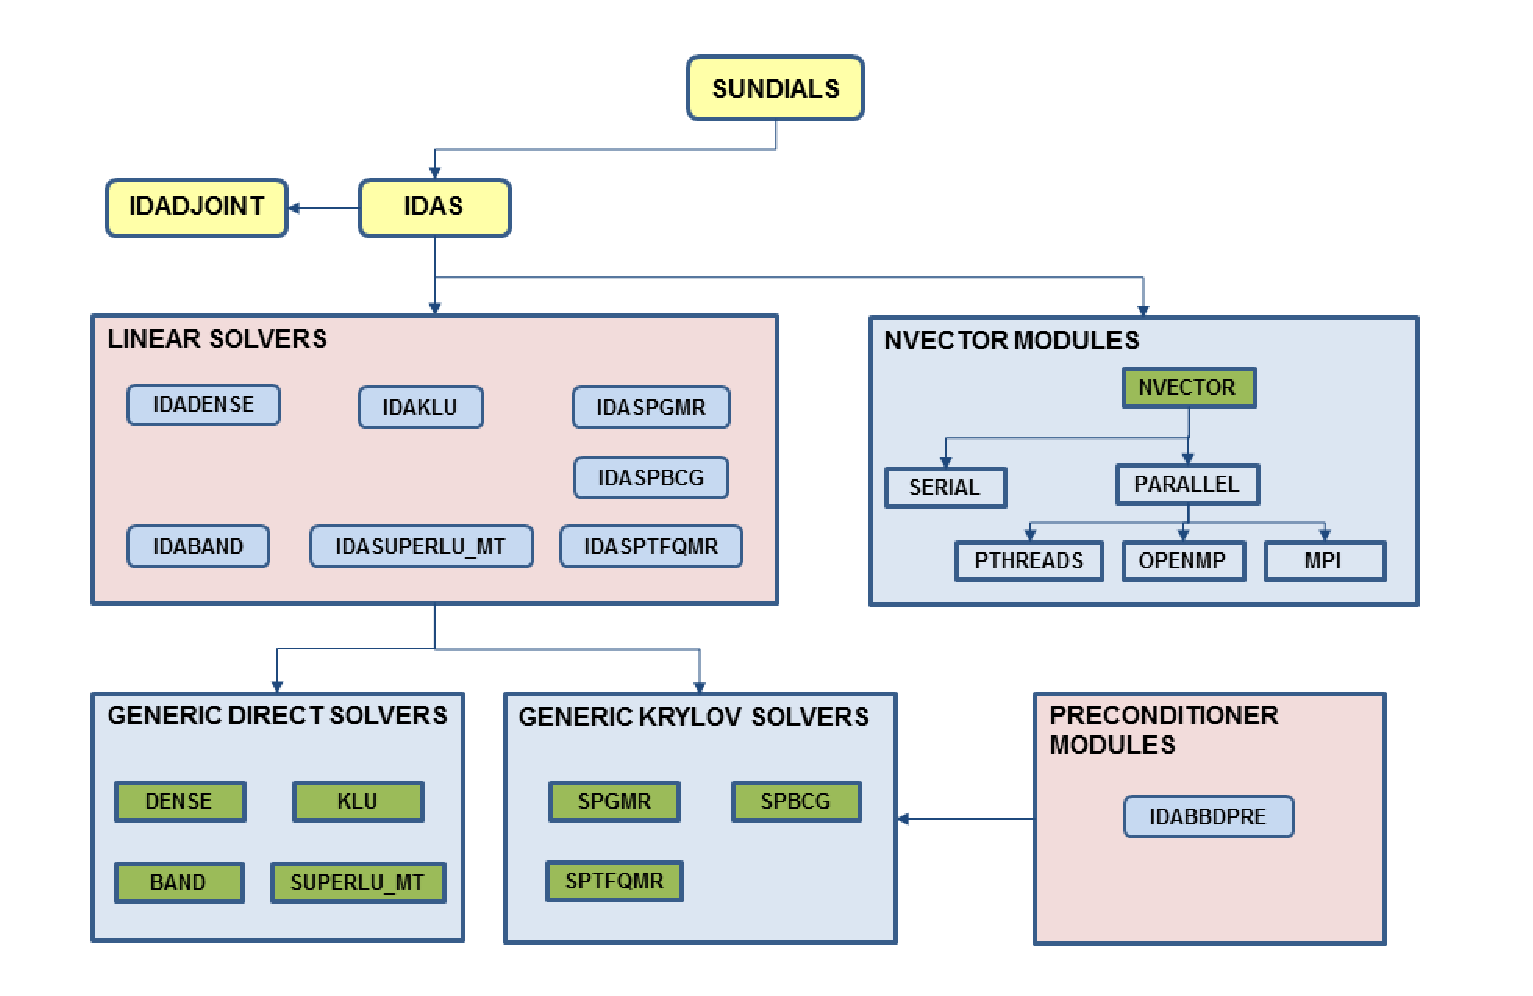
\includegraphics[width=\textwidth]{idasorg}}}
\caption [Overall structure diagram of the {\idas} package]
{Overall structure diagram of the {\idas} package.
  Modules specific to {\idas} begin with ``IDA'' ({\idals}, {\idanls}, and
  {\idabbdpre}), all other items correspond to generic
  {\sundials} vector, matrix, and solver modules (see Figure \ref{f:sunorg1}).}
\label{f:idasorg}
\end{figure}
The central integration module, implemented in the files \id{idas.h},
\id{idas\_impl.h}, and \id{idas.c}, deals with the evaluation of integration
coefficients, estimation of local error,
selection of stepsize and order, and interpolation to user output
points, among other issues.

{\idas} utilizes generic linear and nonlinear solver modules defined by the
{\sunlinsol} API (see Chapter \ref{s:sunlinsol}) and {\sunnonlinsol} API (see
Chapter \ref{c:sunnonlinsol}) respectively. As such, {\idas} has no knowledge
of the method being used to solve the linear and nonlinear systems that
arise in each time step. For any given user problem, there exists a single
nonlinear solver interface and, if necessary, one of the linear system solver
interfaces is specified, and invoked as needed during the integration. While
{\sundials} includes a fixed-point nonlinear solver module, it is not currently
supported in {\idas} (note the fixed-point module is listed in Figure
\ref{f:sunorg1} but not Figure \ref{f:idasorg}).

In addition, if forward sensitivity analysis is turned on, the main module
will integrate the forward sensitivity equations simultaneously with the original
IVP. The sensitivity variables may be included in the local error control
mechanism of the main integrator.
\index{forward sensitivity analysis!correction strategies}
{\idas} provides two different strategies for dealing with the correction
stage for the sensitivity variables: \Id{IDA\_SIMULTANEOUS} \Id{IDA\_STAGGERED}
(see \S\ref{ss:fwd_sensi}).
The {\idas} package includes an algorithm for the approximation of the
sensitivity equations residuals by difference quotients, but the user has
the option of supplying these residual functions directly.

\index{adjoint sensitivity analysis!implementation in {\idas}|(}
The adjoint sensitivity module (file \id{idaa.c}) provides the infrastructure needed for the
backward integration of any system of DAEs which depends on the solution
of the original IVP, in particular the adjoint system and any quadratures required
in evaluating the gradient of the objective functional.  This module deals with
the setup of the checkpoints, the interpolation of the forward solution during
the backward integration, and the backward integration of the adjoint equations.
\index{adjoint sensitivity analysis!implementation in {\idas}|)}

\index{IDAS@{\ida} linear solver interfaces|(}
{\idas} now has a single unified linear solver interface, {\idals},
supporting both direct and iterative linear solvers built using the
generic {\sunlinsol} API (see Chapter \ref{s:sunlinsol}).  These
solvers may utilize a {\sunmatrix} object (see Chapter
\ref{s:sunmatrix}) for storing Jacobian information, or they may be
matrix-free.  Since {\idas} can operate on any valid {\sunlinsol}
implementation, the set of linear solver modules available to {\idas}
will expand as new {\sunlinsol} modules are developed.

For users employing dense or banded Jacobian matrices, {\idals}
includes algorithms for their approximation through difference
quotients, but the user also has the option of supplying the Jacobian
(or an approximation to it) directly.  This user-supplied
routine is required when using sparse or user-supplied Jacobian
matrices.

For users employing matrix-free iterative linear solvers, {\idals}
includes an algorithm for the approximation by difference quotients of
the product between the Jacobian matrix and a vector, $Jv$. Again, the
user has the option of providing routines for this operation, in two
phases: setup (preprocessing of Jacobian data) and multiplication.

For preconditioned iterative methods, \index{preconditioning!setup and solve phases}
the preconditioning must be supplied by the user, again in two phases:
setup and solve.  While\index{preconditioning!advice on} there is no
default choice of preconditioner analogous to the difference-quotient
approximation in the direct case, the references
\cite{BrHi:89,Byr:92}, together with the example and demonstration
programs included with {\idas}, offer considerable assistance in
building preconditioners.

\index{IDAS@{\idas} linear solvers!implementation details|(}
{\idas}' linear solver interface consists of four primary routines,
devoted to (1) memory allocation and initialization, (2) setup of the
matrix data involved, (3) solution of the system, and (4) freeing of memory.
The setup and solution phases are separate because the evaluation of
Jacobians and preconditioners is done only periodically during the
integration, as required to achieve convergence. The call list within
the central {\idas} module to each of the four associated functions is
fixed, thus allowing the central module to be completely independent
of the linear system method.
\index{IDAS@{\idas} linear solvers!implementation details|)}

{\idas} also provides a preconditioner module, {\idabbdpre}, for use
with any of the Krylov iterative linear solvers.  It works in
conjunction with {\nvecp} and generates a preconditioner that is a
block-diagonal matrix with each block being a banded matrix.

All state information used by {\idas} to solve a given problem is saved
in a structure, and a pointer to that structure is returned to the
user.  There is no global data in the {\idas} package, and so, in this
respect, it is reentrant. State information specific to the linear
solver is saved in a separate structure, a pointer to which resides in
the {\idas} memory structure. The reentrancy of {\idas} was motivated
by the situation where two or more problems are solved by
intermixed calls to the package from one user program.

\clearemptydoublepage
%===============================================================
% Usage for simulation
%%==================================================================================
\chapter{Using IDAS for IVP Solution}\label{s:simulation}
%%===================================================================================

This chapter is concerned with the use of {\idas} for the integration
of DAEs in a C language setting.  The following sections treat the header files,
the layout of the user's main program, description of the {\idas} user-callable
functions, and description of user-supplied functions.
This usage is essentially equivalent to using {\ida}~\cite{ida_ug}.

The sample programs described in the companion document \cite{idas_ex}
may also be helpful. Those codes may be used as templates (with the removal of
some lines involved in testing), and are included in the {\idas} package.

The user should be aware that not all {\sunlinsol} and {\sunmatrix}
modules are compatible with all {\nvector} implementations.
\index{IDAS@{\idas} linear solvers!NVECTOR@{\nvector} compatibility}
Details on compatibility are given in the documentation for each
{\sunmatrix} module (Chapter \ref{s:sunmatrix}) and each {\sunlinsol}
module (Chapter \ref{s:sunlinsol}). For example, {\nvecp} is not
compatible with the dense, banded, or sparse {\sunmatrix} types, or with
the corresponding dense, banded, or sparse {\sunlinsol} modules.  Please
check Chapters \ref{s:sunmatrix} and \ref{s:sunlinsol} to verify
compatibility between these modules.  In addition to that
documentation, we note that the preconditioner module {\idabbdpre}
can only be used with {\nvecp}.
It is not recommended to use a threaded vector module with SuperLU\_MT
unless it is the {\nvecopenmp} module, and SuperLU\_MT is also compiled
with OpenMP.

{\idas} uses various constants for both input and output.  These are
defined as needed in this chapter, but for convenience are also listed
separately in Appendix \ref{c:constants}.

%%==============================================================================
\section{Access to library and header files}\label{ss:file_access}
%%==============================================================================

At this point, it is assumed that the installation of {\idas},
following the procedure described in Appendix \ref{c:install}, has
been completed successfully.

Regardless of where the user's application program resides, its
associated compilation and load commands must make reference to the
appropriate locations for the library and header files required by
{\idas}.  The relevant library files are
\begin{itemize}
\item {\em libdir}\id{/libsundials\_idas.}{\em lib},
\item {\em libdir}\id{/libsundials\_nvec*.}{\em lib},
\end{itemize}
where the file extension .{\em lib} is typically \id{.so} for shared libraries
and \id{.a} for static libraries. The relevant header files are located in
the subdirectories
\begin{itemize}
\item {\em incdir}\id{/include/idas}
\item {\em incdir}\id{/include/sundials}
\item {\em incdir}\id{/include/nvector}
\item {\em incdir}\id{/include/sunmatrix}
\item {\em incdir}\id{/include/sunlinsol}
\item {\em incdir}\id{/include/sunnonlinsol}
\end{itemize}
The directories {\em libdir} and {\em incdir} are the install library
and include directories, respectively. For a default installation,
these are {\em instdir}\id{/lib} and {\em instdir}\id{/include},
respectively, where {\em instdir} is the directory where {\sundials}
was installed (see Appendix \ref{c:install}).

Note that an application cannot link to both the {\ida} and {\idas} libraries
because both contain user-callable functions with the same names (to ensure that {\idas}
is backward compatible with {\ida}). Therefore, applications that contain both
DAE problems and DAEs with sensitivity analysis, should use {\idas}.

%%===================================================================================
\section{Data types}\label{s:types}
%%===================================================================================
% This is a shared SUNDIALS TEX file with description of
% types used in llntyps.h
%
\section{Description}

The \ID{sundialstypes.h} file contains the definitions of the types \id{realtype} and
\id{integertype}. {\sundials} solvers use the type \id{realtype} for all floating point data and
the type \id{integertype} for all problem size-related data such as the actual
problem size, the bandwidths in the {\band} solver, and the integers
stored in the length $N$ pivot arrays in both the {\dense} and {\band} solvers.
These types make it easy to solve problems of virtually any size
using single or double precision arithmetic. The type \id{realtype} can be
\id{double} or \id{float} and the type \id{integertype} can be \id{int} or
\id{long int}. The default settings are \id{double} and \id{long int}.

\section{Changing Type \id{realtype}}

The user can change the precision of the {\sundials} solvers arithmetic from double to single
by changing the typedef \id{typedef double realtype;} to \id{typedef float realtype;}
and by changing in \id{sundialstypes.h} the definitions
\begin{verbatim}
#define SUNDIALS_FLOAT  0
#define SUNDIALS_DOUBLE 1
\end{verbatim}
to
\begin{verbatim}
#define SUNDIALS_FLOAT  1
#define SUNDIALS_DOUBLE 0
\end{verbatim}
%\id{\#define SUNDIALS\_FLOAT  0} to \id{\#define SUNDIALS\_FLOAT  1}
%and \id{\#define SUNDIALS\_DOUBLE 1} to \id{\#define SUNDIALS\_DOUBLE 0}
%in \id{sundialstypes.h}.
These macro definitions are used to enable \id{sundiastypes.h} to branch on
the setting of \id{realtype} at compile time. 

Changing from double precision to single precision arithmetic also
requires minor changes in the implementation file \id{sundialsmath.c} for
the {\sundialsmath} module which {\sundials} solvers use. The \id{RPowerR} and
\id{RSqrt} functions compute a real number raised to a real power and the
square root of a number, respectively. The default implementation of
these routines calls standard {\C} math library functions which do double
precision arithmetic. These implementations should be changed to call
single precision routines which are available on the user's machine.

Within {\sundials}, real constants are set by way of a macro called
\Id{RCONST}.  It is this macro that needs the ability to branch on the
setting for \id{realtype}.  In ANSI {\C}, a floating point constant with no
suffix is stored as a \id{double}.  Placing the suffix ``F'' at the
end of a floating point constant makes it a \id{float}. For example,
\begin{verbatim}
#define A 1.0
#define B 1.0F
\end{verbatim}
defines \id{A} to be a \id{double} constant 1.0 and \id{B} to be a
\id{float} constant $1.0$. The macro call \id{RCONST(1.0)}
expands to \id{1.0} if \id{realtype} is \id{double} and it expands to
\id{1.0F} if \id{realtype} is \id{float}. {\sundials} uses the \id{RCONST} macro for
all its floating point constants. 

A user program which uses the type \id{realtype} and the \id{RCONST} macro
to handle floating point constants is precision-independent except for
any calls to single or double precision standard math library
functions.  (Our demonstration programs use \id{realtype} but not
\id{RCONST}.)  Users can, however, use the type \id{double} or
\id{float} in their code (assuming the typedef for \id{realtype} matches
this choice).  Thus, a previously existing piece of ANSI {\C} code can use
{\sundials} without modifying the codes to use \id{realtype}.

\section{Changing Type \id{integertype}}

{\sundials} uses the type \id{integertype} for all quantities related to problem
size.  On some machines the size of an \id{int} and a \id{long int}
are the same, but this is not always the case. 
If \id{int} is sufficiently large on a given machine, and the user wishes
to make \id{int} the \id{integertype} type, change the typedef
\id{typedef long int integertype;} to \id{typedef int integertype;}
and the macro definitions in \id{sundialstypes.h}
\begin{verbatim}
#define SUNDIALS_INT      0
#define SUNDIALS_LONG_INT 1
\end{verbatim}
to
\begin{verbatim}
#define SUNDIALS_INT      1
#define SUNDIALS_LONG_INT 0
\end{verbatim}
%\id{\#define SUNDIALS\_INT 0} to \id{\#define SUNDIALS\_INT 1}
%and
%\id{\#define SUNDIALS\_LONG\_INT 1} to \id{\#define SUNDIALS\_LONG\_INT 0}
%in \id{sundialstypes.h}.
In terms of the problem size $N$, and the bandwidths \id{ml} and \id{mu} 
in the case of the band module {\band}, the largest integer that must be 
accommodated by the \id{integertype} type is $N + $ \id{ml} + \id{mu} in the 
band case, and $N$ in all other cases. The user can use the type \id{int} 
or \id{long int} in his/her code instead of \id{integertype} (assuming the 
typedef for \id{integertype} matches this choice).

%%===================================================================================
\section{Header files}\label{ss:header_sim}
%%===================================================================================
\index{header files}
The calling program must include several header files so that various macros
and data types can be used. The header file that is always required is:
%%
\begin{itemize}
\item  \Id{idas/idas.h},
  the header file for {\idas}, which defines the several
  types and various constants, and includes function prototypes.  This
  includes the header file for {\idals}, \Id{ida/ida\_ls.h}.
\end{itemize}
%%
Note that \id{idas.h} includes \Id{sundials\_types.h},
which defines the types \id{realtype}, \id{sunindextype}, and \id{booleantype}
and the constants \id{SUNFALSE} and \id{SUNTRUE}.

The calling program must also include an {\nvector} implementation header file,
of the form \\ \noindent
\id{nvector/nvector\_***.h}.  See Chapter \ref{s:nvector} for the appropriate
name.  This file in turn includes the header file \Id{sundials\_nvector.h}
which defines the abstract \Id{N\_Vector} data type.

If using a non-default nonlinear solver module, or when interacting
with a {\sunnonlinsol} module directly, the calling program must also
include a {\sunnonlinsol} implementation header file, of the form
\id{sunnonlinsol/sunnonlinsol\_***.h} where \id{***} is the name of the
nonlinear solver module (see Chapter \ref{c:sunnonlinsol} for more
information). This file in turn includes the header file
\Id{sundials\_nonlinearsolver.h} which defines the abstract
\Id{SUNNonlinearSolver} data type.

If using a nonlinear solver that requires the solution of a linear
system of the form (\ref{e:DAE_Newtoncorr}) (e.g., the default Newton
iteration), a linear solver module header file is also required.
\index{IDAS@{\idas} linear solvers!header files}
The header files corresponding to the various {\sundials}-provided
linear solver modules available for use with {\idas} are: 
%%
\begin{itemize}
\item Direct linear solvers:
  \begin{itemize}
  \item \Id{sunlinsol/sunlinsol\_dense.h},
    which is used with the dense linear solver module,
    {\sunlinsoldense};

  \item \Id{sunlinsol/sunlinsol\_band.h},
    which is used with the banded linear solver module,
    {\sunlinsolband};

  \item \Id{sunlinsol/sunlinsol\_lapackdense.h},
    which is used with the LAPACK dense linear solver module,
    {\sunlinsollapdense};

  \item \Id{sunlinsol/sunlinsol\_lapackband.h},
    which is used with the LAPACK banded linear solver module,
    {\sunlinsollapband};

  \item \Id{sunlinsol/sunlinsol\_klu.h},
    which is used with the {\klu} sparse linear solver module,
    {\sunlinsolklu};

  \item \Id{sunlinsol/sunlinsol\_superlumt.h},
    which is used with the {\superlumt} sparse linear solver
    module, {\sunlinsolslumt};
  \end{itemize}

\item Iterative linear solvers:
  \begin{itemize}
  \item \Id{sunlinsol/sunlinsol\_spgmr.h},
    which is used with the scaled, preconditioned GMRES Krylov linear
    solver module, {\sunlinsolspgmr};

  \item \Id{sunlinsol/sunlinsol\_spfgmr.h},
    which is used with the scaled, preconditioned FGMRES Krylov linear
    solver module, {\sunlinsolspfgmr};

  \item \Id{sunlinsol/sunlinsol\_spbcgs.h},
    which is used with the scaled, preconditioned Bi-CGStab Krylov
    linear solver module, {\sunlinsolspbcgs};

  \item \Id{sunlinsol/sunlinsol\_sptfqmr.h},
    which is used with the scaled, preconditioned TFQMR Krylov linear
    solver module, {\sunlinsolsptfqmr};

  \item \Id{sunlinsol/sunlinsol\_pcg.h},
    which is used with the scaled, preconditioned CG Krylov linear
    solver module, {\sunlinsolpcg};
  \end{itemize}
\end{itemize}

The header files for the {\sunlinsoldense} and {\sunlinsollapdense}
linear solver modules include the file
\id{sunmatrix/sunmatrix\_dense.h}, which defines the {\sunmatdense}
matrix module, as as well as various functions and macros acting on
such matrices.

The header files for the {\sunlinsolband} and {\sunlinsollapband}
linear solver modules include the file
\id{sunmatrix/sunmatrix\_band.h}, which defines the {\sunmatband}
matrix module, as as well as various functions and macros acting on
such matrices.

The header files for the {\sunlinsolklu} and {\sunlinsolslumt}
sparse linear solvers include the file
\id{sunmatrix/sunmatrix\_sparse.h}, which defines the {\sunmatsparse}
matrix module, as well as various functions and macros acting on such
matrices.

The header files for the Krylov iterative solvers include the file
\id{sundials/sundials\_iterative.h}, which enumerates the kind of
preconditioning, and (for the {\spgmr} and {\spfgmr} solvers) the
choices for the Gram-Schmidt process.

Other headers may be needed, according to the choice of
preconditioner, etc.  For example, in the \id{idasFoodWeb\_kry\_p}
example (see \cite{idas_ex}), preconditioning is done with a
block-diagonal matrix. For this, even though the {\sunlinsolspgmr}
linear solver is used, the header \id{sundials/sundials\_dense.h} is
included for access to the underlying generic dense matrix arithmetic
routines.

%%====================================================================
\section{A skeleton of the user's main program}\label{ss:skeleton_sim}
%%====================================================================
The following is a skeleton of the user's main program (or calling program)
for the integration of a DAE IVP. Most of the steps are independent of the
{\nvector}, {\sunmatrix}, {\sunlinsol}, and {\sunnonlinsol} implementations
used. For the steps that are not, refer to Chapter \ref{s:nvector},
\ref{s:sunmatrix}, \ref{s:sunlinsol}, and \ref{c:sunnonlinsol} for the specific
name of the function to be called or macro to be referenced.
%%
\index{User main program!IDAS@{\idas} usage}
\begin{Steps}

\item
  {\bf Initialize parallel or multi-threaded environment, if appropriate}

  For example, call \id{MPI\_Init} to initialize {\mpi} if used, or
  set \id{num\_threads}, the number of threads to use within the threaded
  vector functions, if used.

\item
  {\bf Set problem dimensions etc.}

  This generally includes the problem size \id{N}, and may include
  the local vector length \id{Nlocal}.

  Note: The variables \id{N} and \id{Nlocal} should be of type \id{sunindextype}.

\item
  {\bf Set vectors of initial values}

  To set the vectors \id{y0} and \id{yp0} to initial values for $y$\ and
  $\dot{y}$, use the appropriate functions defined by the particular
  {\nvector} implementation.

  For native {\sundials} vector implementations
  (except the {\cuda} and {\raja}-based ones),
  use a call of the form \id{y0 = N\_VMake\_***(..., ydata)} if the \id{realtype}
  array \id{ydata} containing the initial values of $y$ already exists.
  Otherwise, create a new vector by making a call of the form
  \id{y0 = N\_VNew\_***(...)}, and then set its elements by accessing
  the underlying data with a call of the form
  \id{ ydata = N\_VGetArrayPointer(y0)}.
  See \S\ref{ss:nvec_ser}-\ref{ss:nvec_pthreads} for details.

  For the {\hypre} and {\petsc} vector wrappers, first create and initialize
  the underlying vector and then create an {\nvector} wrapper with a call
  of the form \id{y0 = N\_VMake\_***(yvec)}, where \id{yvec} is a {\hypre}
  or {\petsc} vector. Note that calls like \id{N\_VNew\_***(...)} and
  \id{N\_VGetArrayPointer(...)} are not available for these vector wrappers.
  See \S\ref{ss:nvec_parhyp} and \S\ref{ss:nvec_petsc} for details.

  If using either the {\cuda}- or {\raja}-based vector implementations
  use a call of the form
  \id{y0 = N\_VMake\_***(..., c)} where \id{c} is a pointer to a \id{suncudavec}
  or \id{sunrajavec} vector class if this class already exists.  Otherwise,
  create a new vector
  by making a call of the form \id{y0 = N\_VNew\_***(...)}, and then set its
  elements by accessing the underlying data where it is located
  with a call of the form
  \id{N\_VGetDeviceArrayPointer\_***} or \id{N\_VGetHostArrayPointer\_***}.
  Note that the vector class will allocate memory on both the host and device
  when instantiated.  See \S\ref{ss:nvec_cuda}-\ref{ss:nvec_raja} for details.

%   If a \id{realtype} array \id{ydata} containing the initial values of $y$
%   already exists, it may be possible to set \id{y0} either with a call of the form
%   \id{y0 = N\_VMake\_***(..., ydata);}
%   or by making a call of the form
%   \id{y0 = N\_VNew\_***(...);}
%   and loading values into the structure defined by \id{NV\_DATA\_***(y0)},
%   provided these functions and macro exist for the {\nvector} module chosen.

  Set the vector \id{yp0} of initial conditions for $\dot{y}$ similarly.

\item\label{i:ida_create}
  {\bf Create {\idas} object}

  Call \id{ida\_mem = }\id{IDACreate}\id{()}
  to create the {\idas} memory block.
  \id{IDACreate} returns a pointer to the {\idas} memory structure.
  See \S\ref{sss:idainit} for details.
  This \id{void *} pointer must then be passed as the first argument
  to all subsequent {\idas} function calls.

\item\label{i:ida_init}
  {\bf Initialize {\idas} solver}

  Call \id{IDAInit}\id{(...)} to provide required problem
  specifications (residual function, initial time, and initial conditions),
  allocate internal memory for {\idas}, and initialize {\idas}.
  \id{IDAInit} returns an error flag to indicate success or an illegal argument
  value.  See \S\ref{sss:idainit} for details.

\item
  {\bf Specify integration tolerances}

  Call \id{IDASStolerances}\id{(...)} or \id{IDASVtolerances}\id{(...)}
  to specify, respectively, a scalar relative tolerance and scalar
  absolute tolerance, or a scalar relative tolerance and a vector of
  absolute tolerances.  Alternatively, call \id{IDAWFtolerances} to
  specify a function which sets directly the weights used in
  evaluating WRMS vector norms.  See \S\ref{sss:idatolerances} for
  details.

\item\label{i:matrix}
  {\bf Create matrix object}

  If a nonlinear solver requiring a linear solver will be used (e.g., the
  default Newton iteration) and the linear solver will be a matrix-based linear
  solver, then a template Jacobian matrix must be created by using the
  appropriate constructor function defined by the particular {\sunmatrix}
  implementation.

  For the {\sundials}-supplied {\sunmatrix} implementations, the
  matrix object may be created using a call of the form

  \id{SUNMatrix J = }\Id{SUNBandMatrix}\id{(...);}

   or

  \id{SUNMatrix J = }\Id{SUNDenseMatrix}\id{(...);}

   or

  \id{SUNMatrix J = }\Id{SUNSparseMatrix}\id{(...);}

  NOTE: The dense, banded, and sparse matrix objects are usable only in a
  serial or threaded environment.

\item\label{i:lin_solver}
  {\bf Create linear solver object}

  If a nonlinear solver requiring a linear solver is chosen (e.g., the default
  Newton iteration), then the desired linear solver object must be created by
  calling the appropriate constructor function defined by the particular
  {\sunlinsol} implementation.

  For any of the {\sundials}-supplied {\sunlinsol} implementations,
  the linear solver object may be created using a call of the form

  \id{SUNLinearSolver LS = SUNLinSol\_*(...);}

  where \id{*} can be replaced with ``Dense'', ``SPGMR'', or other
  options, as discussed in \S\ref{sss:lin_solv_init} and Chapter {\ref{s:sunlinsol}}.

\item
  {\bf Set linear solver optional inputs}

  Call \id{*Set*} functions from the selected linear solver module
  to change optional inputs specific to that linear solver.
  See the documentation for each {\sunlinsol} module in Chapter
  {\ref{s:sunlinsol}} for details.

\item\label{i:lin_solver_interface}
  {\bf Attach linear solver module}

  If a nonlinear solver requiring a linear solver is chosen (e.g., the default
  Newton iteration), then initialize the {\idals} linear solver
  interface by attaching the linear solver object (and matrix object, if
  applicable) with the following call (for details see
  \S\ref{sss:lin_solv_init}):

  \id{ier = }\Id{IDASetLinearSolver}\id{(...);}

\item
  {\bf Set optional inputs}

  Optionally, call \id{IDASet*} functions to change from their default values any
  optional inputs that control the behavior of {\idas}.
  See \S\ref{sss:optin_main} and \S\ref{ss:optional_input} for details.

\item\label{i:nonlin_solver}
  {\bf Create nonlinear solver object} (\textit{optional})

  If using a non-default nonlinear solver (see \S\ref{sss:nonlin_solv_init}),
  then create the desired nonlinear solver object by calling the appropriate
  constructor function defined by the particular {\sunnonlinsol} implementation
  (e.g., \id{NLS = SUNNonlinSol\_***(...);} where \id{***} is the name of the
  nonlinear solver (see Chapter \ref{c:sunnonlinsol} for details).

\item\label{i:nonlin_solver_interface}
  {\bf Attach nonlinear solver module} (\textit{optional})

  If using a non-default nonlinear solver, then initialize the nonlinear solver
  interface by attaching the nonlinear solver object by calling
  \id{ier = }\Id{IDASetNonlinearSolver}\id{(ida\_mem, NLS);} (see
  \S\ref{sss:nonlin_solv_init} for details).

\item
  {\bf Set nonlinear solver optional inputs} (\textit{optional})

  Call the appropriate set functions for the selected nonlinear solver module to
  change optional inputs specific to that nonlinear solver. These \textit{must}
  be called after \id{IDAInit} if using the default nonlinear solver or after
  attaching a new nonlinear solver to {\idas}, otherwise the optional inputs will
  be overridden by {\idas} defaults. See Chapter \ref{c:sunnonlinsol} for more
  information on optional inputs.

\item
  {\bf Correct initial values}

  Optionally, call \id{IDACalcIC} to correct the initial values
  \id{y0} and \id{yp0} passed to \id{IDAInit}.  See \S\ref{ss:idacalcic}.
  Also see \S\ref{sss:optin_iccalc} for relevant optional input calls.

\item
  {\bf Specify rootfinding problem}
  \index{Rootfinding}

  Optionally, call \id{IDARootInit} to initialize a rootfinding problem
  to be solved during the integration of the DAE system.
  See \S\ref{ss:idarootinit} for details, and see \S\ref{sss:optin_root}
  for relevant optional input calls.

\item
  {\bf Advance solution in time}

  For each point at which output is desired, call
  \id{flag = }\Id{IDASolve}\id{(ida\_mem, tout, \&tret, yret, ypret, itask)}.
  Here \id{itask} specifies the return mode.  The vector \id{yret}
  (which can be the same as the vector \id{y0} above) will contain $y(t)$,
  while the vector \id{ypret} (which can be the same as the vector \id{yp0}
  above) will contain $\dot{y}(t)$.
  See \S\ref{sss:idasolve} for details.

\item
  {\bf Get optional outputs}

  Call \id{IDA*Get*} functions to obtain optional output.
  See \S\ref{ss:optional_output} for details.

\item
  {\bf Deallocate memory for solution vectors}

  Upon completion of the integration, deallocate memory for the vectors \id{yret}
  and \id{ypret} (or \id{y} and \id{yp}) by calling the appropriate destructor
  function defined by the {\nvector} implementation:

  \id{N\_VDestroy(yret);}

  and similarly for \id{ypret}.

\item
  {\bf Free solver memory}

  \Id{IDAFree}\id{(\&ida\_mem)} to free the memory allocated for {\idas}.

\item
  {\bf Free nonlinear solver memory} (\textit{optional})

  If a non-default nonlinear solver was used, then call
  \Id{SUNNonlinSolFree}\id{(NLS)} to free any memory allocated for the
  {\sunnonlinsol} object.

\item
  {\bf Free linear solver and matrix memory}

  Call \Id{SUNLinSolFree} and \ID{SUNMatDestroy} to free any memory
  allocated for the linear solver and matrix objects created above.

\item
  {\bf Finalize MPI, if used}

  Call \id{MPI\_Finalize()} to terminate MPI.

\end{Steps}

{\sundials} provides some linear solvers only as a means for 
users to get problems running and not as highly efficient solvers.
In particular, the dense and band direct solvers are not nearly as efficient as
their LAPACK counterparts, and users are encouraged to use LAPACK solvers
if an efficient dense direct solver is needed.
Table \ref{t:solver-vector} shows the linear solver interfaces
available in {\sundials} packages and the vector implementations
required for use.  As an example, one cannot use the {\sundials} package
specific dense direct
solver interfaces  with the \mpi-based vector implementation.  However, 
as discussed in Chapter \ref{s:gen_linsolv} the direct dense, direct band, 
and iterative spils solvers provided with
{\sundials} are written in a way that allows a user to develop 
their own solvers around them should a user so desire.  

\begin{table}[htb]
  %\xentrystretch{2.5}
  \centering
    \caption{{\sundials} linear solver interfaces and vector 
             implementations that can be used for each.}
    \medskip
    \tablefirsthead{\hline \multicolumn{1}{|p{2cm}|}{{Linear Solver Interface}} &
                           \multicolumn{1}{p{1.3cm}|}{{Serial}} & 
                           \multicolumn{1}{p{1.3cm}|}{{Parallel (MPI)}} & 
                           \multicolumn{1}{p{1.4cm}|}{{OpenMP}} & 
                           \multicolumn{1}{p{1.4cm}|}{{pThreads}} & 
                           \multicolumn{1}{p{1.3cm}|}{{{\hypre} Vector}} & 
                           \multicolumn{1}{p{1.3cm}|}{{{\petsc} Vector}} & 
                           \multicolumn{1}{p{1.4cm}|}{{User Supplied}} \\ \hline }
    {\renewcommand{\arraystretch}{1.2}
    \begin{xtabular}{|l|c|c|c|c|c|c|c|}
%   Linear Solver &  Serial  & Parallel  &  OpenMP  &  pThreads  & {\hypre}    & {\petsc} & User     \\
%   Interface     &          & (MPI)     &          &            &  Vector     & Vector   & Supplied \\ 
    Dense         &  \cm     &           & \cm      &  \cm       &             &          & \cm      \\ 
    Band          &  \cm     &           & \cm      &  \cm       &             &          & \cm      \\
    LapackDense   &  \cm     &           & \cm      &  \cm       &             &          & \cm      \\
    LapackBand    &  \cm     &           & \cm      &  \cm       &             &          & \cm      \\
    \klu          &  \cm     &           & \cm      &  \cm       &             &          & \cm      \\
    \superlumt    &  \cm     &           & \cm      &  \cm       &             &          & \cm      \\
    \spgmr        &  \cm     &  \cm      &  \cm     &  \cm       & \cm         &  \cm     & \cm      \\
    \spfgmr       &  \cm     &  \cm      &  \cm     &  \cm       & \cm         &  \cm     & \cm      \\
    \spbcg        &  \cm     &  \cm      &  \cm     &  \cm       & \cm         &  \cm     & \cm      \\
    \sptfqmr      &  \cm     &  \cm      &  \cm     &  \cm       & \cm         &  \cm     & \cm      \\ 
    User supplied &  \cm     &  \cm      &  \cm     &  \cm       & \cm         &  \cm     & \cm      \\ 
    \hline
    \end{xtabular}
    }
    \label{t:solver-vector}
\end{table}



%%==========================================================
\section{User-callable functions}\label{ss:callable_fct_sim}
%%==========================================================

This section describes the {\idas} functions that are called by the
user to set up and solve a DAE. Some of these are required. However,
starting with \S\ref{ss:optional_input}, the functions listed involve
optional inputs/outputs or restarting, and those paragraphs can be
skipped for a casual use of {\idas}. In any case, refer to
\S\ref{ss:skeleton_sim} for the correct order of these calls.

On an error, each user-callable function returns a negative value and
sends an error message to the error handler routine, which prints the
message on \id{stderr} by default. However, the user can set a file
as error output or can provide his own error handler function (see
\S\ref{sss:optin_main}).

\subsection{IDAS initialization and deallocation functions}
\label{sss:idainit}
%%
The following three functions must be called in the order listed. The last one
is to be called only after the DAE solution is complete, as it frees the {\idas}
memory block created and allocated by the first two calls.
%%
\ucfunction{IDACreate}
{
  ida\_mem = IDACreate();
}
{
  The function \ID{IDACreate} instantiates an {\idas} solver object.
}
{
  \id{IDACreate} has no arguments.
}
{
  If successful, \id{IDACreate} returns a pointer to the newly created
  {\idas} memory block (of type \id{void *}).  Otherwise it returns \id{NULL}.
}
{}
%%
%%
\ucfunction{IDAInit}
{
  flag = IDAInit(ida\_mem, res, t0, y0, yp0);
}
{
  The function \ID{IDAInit} provides required problem and solution
  specifications, allocates internal memory, and initializes {\idas}.
}
{
  \begin{args}[ida\_mem]
  \item[ida\_mem] (\id{void *})
    pointer to the {\idas} memory block returned by \id{IDACreate}.
  \item[res] (\Id{IDAResFn})
    is the {\CC} function which computes the residual function $F$ in the DAE.
     This function has the form \id{res(t, yy, yp, resval, user\_data)}.
     For full details see \S\ref{ss:resFn}.
  \item[t0] (\id{realtype})
    is the initial value of $t$.
  \item[y0] (\id{N\_Vector})
    is the initial value of $y$.
  \item[yp0] (\id{N\_Vector})
    is the initial value of $\dot{y}$.
  \end{args}
}
{
  The return value \id{flag} (of type \id{int}) will be one of the following:
  \begin{args}[IDA\_ILL\_INPUT]
  \item[\Id{IDA\_SUCCESS}]
    The call to \id{IDAInit} was successful.
  \item[\Id{IDA\_MEM\_NULL}]
    The {\idas} memory block was not initialized through a previous call to
    \id{IDACreate}.
  \item[\Id{IDA\_MEM\_FAIL}]
    A memory allocation request has failed.
  \item[\Id{IDA\_ILL\_INPUT}]
    An input argument to \id{IDAInit} has an illegal value.
  \end{args}
}
{
  If an error occurred, \id{IDAInit} also sends an error message to the
  error handler function.
}
%%
%%
\ucfunction{IDAFree}
{
  IDAFree(\&ida\_mem);
}
{
  The function \ID{IDAFree} frees the pointer allocated by
  a previous call to \id{IDACreate}.
}
{
  The argument is the pointer to the {\idas} memory block (of type \id{void *}).
}
{
  The function \id{IDAFree} has no return value.
}
{}


%%==============================================================================
\subsection{IDAS tolerance specification functions}\label{sss:idatolerances}
%%==============================================================================
%%
One of the following three functions must be called to specify the
integration tolerances (or directly specify the weights used in
evaluating WRMS vector norms).  Note that this call must be made after
the call to \id{IDAInit}.
%%
\ucfunction{IDASStolerances}
{
  flag = IDASStolerances(ida\_mem, reltol, abstol);
}
{
  The function \ID{IDASStolerances} specifies scalar relative and absolute
  tolerances.
}
{
  \begin{args}[ida\_mem]
  \item[ida\_mem] (\id{void *})
    pointer to the {\idas} memory block returned by \id{IDACreate}.
  \item[reltol] (\id{realtype})
    is the scalar relative error tolerance.
  \item[abstol] (\id{realtype})
    is the scalar absolute error tolerance.
  \end{args}
}
{
  The return value \id{flag} (of type \id{int}) will be one of the following:
  \begin{args}[IDA\_ILL\_INPUT]
  \item[\Id{IDA\_SUCCESS}]
    The call to \id{IDASStolerances} was successful.
  \item[\Id{IDA\_MEM\_NULL}]
    The {\idas} memory block was not initialized through a previous call to
    \id{IDACreate}.
  \item[\Id{IDA\_NO\_MALLOC}]
    The allocation function \id{IDAInit} has not been called.
  \item[\Id{IDA\_ILL\_INPUT}]
    One of the input tolerances was negative.
  \end{args}
}
{}
%%
%%
\ucfunction{IDASVtolerances}
{
  flag = IDASVtolerances(ida\_mem, reltol, abstol);
}
{
  The function \ID{IDASVtolerances} specifies scalar relative tolerance and
  vector absolute tolerances.
}
{
  \begin{args}[ida\_mem]
  \item[ida\_mem] (\id{void *})
    pointer to the {\idas} memory block returned by \id{IDACreate}.
  \item[reltol] (\id{realtype})
    is the scalar relative error tolerance.
  \item[abstol] (\id{N\_Vector})
    is the vector of absolute error tolerances.
  \end{args}
}
{
  The return value \id{flag} (of type \id{int}) will be one of the following:
  \begin{args}[IDA\_ILL\_INPUT]
  \item[\Id{IDA\_SUCCESS}]
    The call to \id{IDASVtolerances} was successful.
  \item[\Id{IDA\_MEM\_NULL}]
    The {\idas} memory block was not initialized through a previous call to
    \id{IDACreate}.
  \item[\Id{IDA\_NO\_MALLOC}]
    The allocation function \id{IDAInit} has not been called.
  \item[\Id{IDA\_ILL\_INPUT}]
    The relative error tolerance was negative or the absolute tolerance
    had a negative component.
  \end{args}
}
{
  This choice of tolerances is important when the absolute error tolerance needs to
  be different for each component of the state vector $y$.
}
%%
%%
\ucfunction{IDAWFtolerances}
{
  flag = IDAWFtolerances(ida\_mem, efun);
}
{
  The function \ID{IDAWFtolerances} specifies a user-supplied function \id{efun}
  that sets the multiplicative error weights $W_i$ for use in the weighted
  RMS norm, which are normally defined by Eq. (\ref{e:errwt}).
}
{
  \begin{args}[ida\_mem]
  \item[ida\_mem] (\id{void *})
    pointer to the {\idas} memory block returned by \id{IDACreate}.
  \item[efun] (\id{IDAEwtFn})
    is the {\CC} function which defines the \id{ewt} vector (see
    \S\ref{ss:ewtsetFn}).
  \end{args}
}
{
  The return value \id{flag} (of type \id{int}) will be one of the following:
  \begin{args}[IDA\_ILL\_INPUT]
  \item[\Id{IDA\_SUCCESS}]
    The call to \id{IDAWFtolerances} was successful.
  \item[\Id{IDA\_MEM\_NULL}]
    The {\idas} memory block was not initialized through a previous call to
    \id{IDACreate}.
  \item[\Id{IDA\_NO\_MALLOC}]
    The allocation function \id{IDAInit} has not been called.
  \end{args}
}
{}

\index{tolerances}
{\bf General advice on choice of tolerances.}
For many users, the appropriate choices for tolerance values in
\id{reltol} and \id{abstol} are a concern.  The following pieces of
advice are relevant.

(1) The scalar relative tolerance \id{reltol} is to be set to control relative
errors.  So \id{reltol}=$10^{-4}$ means that errors are controlled to .01\%.  We
do not recommend using \id{reltol} larger than $10^{-3}$.  On the other hand,
\id{reltol} should not be so small that it is comparable to the unit roundoff
of the machine arithmetic (generally around $10^{-15}$).

(2) The absolute tolerances \id{abstol} (whether scalar or vector) need to
be set to control absolute errors when any components of the solution
vector \id{y} may be so small that pure relative error control is
meaningless.  For example, if \id{y[i]} starts at some nonzero value, but in time
decays to zero, then pure relative error control on \id{y[i]} makes no sense
(and is overly costly) after \id{y[i]} is below some noise level.  Then
\id{abstol} (if scalar) or \id{abstol[i]} (if a vector) needs to be set to that
noise level.  If the different components have different noise levels,
then \id{abstol} should be a vector.  See the example \id{idasRoberts\_dns} in the
{\idas} package, and the discussion of it in the {\idas} Examples document
\cite{idas_ex}.
In that problem, the three components vary between 0 and 1, and have
different noise levels; hence the \id{abstol} vector.  It is impossible to
give any general advice on \id{abstol} values, because the appropriate noise
levels are completely problem-dependent.  The user or modeler hopefully has
some idea as to what those noise levels are.

(3) Finally, it is important to pick all the tolerance values conservatively,
because they control the error committed on each individual time step.
The final (global) errors are a sort of accumulation of those
per-step errors.  A good rule of thumb is to reduce the tolerances by a
factor of .01 from the actual desired limits on errors.  So if you
want .01\% accuracy (globally), a good choice is \id{reltol}$=10^{-6}$.
But in any case, it is a good idea to do a few experiments with
the tolerances to see how the computed solution values vary as
tolerances are reduced.

\vspace{0.1in}
\index{tolerances}
{\bf Advice on controlling unphysical negative values.}
In many applications, some components in the true solution are always
positive or non-negative, though at times very small.  In the numerical
solution, however, small negative (hence unphysical) values can then
occur.  In most cases, these values are harmless, and simply need to
be controlled, not eliminated. The following pieces of advice are relevant.

(1) The way to control the size of unwanted negative computed values
is with tighter absolute tolerances.  Again this requires some
knowledge of the noise level of these components, which may or may not
be different for different components.  Some experimentation may be
needed.

(2) If output plots or tables are being generated, and it is important
to avoid having negative numbers appear there (for the sake of avoiding
a long explanation of them, if nothing else), then eliminate them, but
only in the context of the output medium.  Then the internal values carried
by the solver are unaffected.  Remember that a small negative value in \id{yret}
returned by {\idas}, with magnitude comparable to \id{abstol} or less,
is equivalent to zero as far as the computation is concerned.

(3) The user's residual routine \id{res} should never change a
negative value in the solution vector \id{yy} to a non-negative value,
as a "solution" to this problem.  This can cause instability.  If the
\id{res} routine cannot tolerate a zero or negative value (e.g., because
there is a square root or log of it), then the offending value should
be changed to zero or a tiny positive number in a temporary variable
(not in the input \id{yy} vector) for the purposes of computing $F(t,y,\dot{y})$.

(4) {\idas} provides the option of enforcing positivity or non-negativity
on components.  Also, such constraints can be enforced by use of the
recoverable error return feature in the user-supplied residual function.
However, because these options involve some extra overhead cost, they
should only be exercised if the use of absolute tolerances to control
the computed values is unsuccessful.
%%
%%==================================================================================
%%
\subsection{Linear solver interface functions}\label{sss:lin_solv_init}

As previously explained, if the nonlinear solver requires the solution of
linear systems of the form (\ref{e:DAE_Newtoncorr}) (e.g., the default Newton
iteration, then solution of these linear systems is handled with the
{\idals} linear solver interface.  This interface supports all valid
{\sunlinsol} modules.  Here, matrix-based {\sunlinsol} modules utilize
{\sunmatrix} objects to store the Jacobian matrix
$J = \partial{F}/\partial{y} + \alpha \partial{F}/\partial{\dot{y}}$
and factorizations used throughout the solution process.  Conversely,
matrix-free {\sunlinsol} modules instead use iterative methods to
solve the linear systems of equations, and only require the
\emph{action} of the Jacobian on a vector, $Jv$.

With most iterative linear solvers, preconditioning can be done on the
left only, on the right only, on both the left and the right, or not
at all.  The exceptions to this rule are {\spfgmr} that supports right
preconditioning only and {\pcg} that performs symmetric
preconditioning.  However, in {\idas} only left preconditioning is
supported.  For the specification of a preconditioner, see the
iterative linear solver sections in \S\ref{ss:optional_input} and
\S\ref{ss:user_fct_sim}. A preconditioner matrix $P$ must approximate
the Jacobian $J$, at least crudely.

\index{IDAS@{\idas} linear solvers!selecting one|(}
To specify a generic linear solver to {\idas}, after the call to
\id{IDACreate} but before any calls to \id{IDASolve}, the user's
program must create the appropriate {\sunlinsol} object and call
the function \Id{IDASetLinearSolver}, as documented below.
To create the \id{SUNLinearSolver} object, the user may call one of
the {\sundials}-packaged {\sunlinsol} module constructor routines via
a call of the form

\begin{verbatim}
      SUNLinearSolver LS = SUNLinSol_*(...);
\end{verbatim}

The current list of such constructor routines includes
\Id{SUNLinSol\_Dense},
\Id{SUNLinSol\_Band},\\ \noindent
\Id{SUNLinSol\_LapackDense},
\Id{SUNLinSol\_LapackBand},
\Id{SUNLinSol\_KLU},
\Id{SUNLinSol\_SuperLUMT},\\ \noindent
\Id{SUNLinSol\_SPGMR},
\Id{SUNLinSol\_SPFGMR},
\Id{SUNLinSol\_SPBCGS},
\Id{SUNLinSol\_SPTFQMR}, and
\Id{SUNLinSol\_PCG}.

Alternately, a user-supplied
\id{SUNLinearSolver} module may be created and used instead.  The use
of each of the generic linear solvers involves certain constants,
functions and possibly some macros, that are likely to be needed in
the user code.  These are available in the corresponding header file
associated with the specific {\sunmatrix} or {\sunlinsol} module in
question, as described in Chapters \ref{s:sunmatrix} and
\ref{s:sunlinsol}.

Once this solver object has been constructed, the user should attach
it to {\idas} via a call to \Id{IDASetLinearSolver}.  The first argument 
passed to this function is the {\idas} memory pointer returned by
\id{IDACreate}; the second argument is the desired {\sunlinsol} object
to use for solving systems.  The third argument is an optional
{\sunmatrix} object to accompany matrix-based {\sunlinsol} inputs (for
matrix-free linear solvers, the third argument should be \id{NULL}).
A call to this function initializes the {\idals} linear solver
interface, linking it to the main {\idas} integrator, and allows the
user to specify additional parameters and routines pertinent to their
choice of linear solver.
\index{IDAS@{\idas} linear solvers!selecting one|)}
%%
\index{IDAS@{\idas} linear solver interface!IDALS@{\idals}}
\ucfunction{IDASetLinearSolver}
{
  flag = IDASetLinearSolver(ida\_mem, LS, J);
}
{
  The function \ID{IDASetLinearSolver} attaches a generic {\sunlinsol}
  object \id{LS} and corresponding template Jacobian {\sunmatrix}
  object \id{J} (if applicable) to {\idas}, initializing the {\idals}
  linear solver interface. 
}
{
  \begin{args}[ida\_mem]
  \item[ida\_mem] (\id{void *})
    pointer to the {\idas} memory block.
  \item[LS] (\id{SUNLinearSolver})
    {\sunlinsol} object to use for solving linear systems of the form
    (\ref{e:DAE_Newtoncorr}.
  \item[J] (\id{SUNMatrix})
    {\sunmatrix} object for used as a template for the Jacobian (or
    \id{NULL} if not applicable).
  \end{args}
}
{
  The return value \id{flag} (of type \id{int}) is one of
  \begin{args}
  [IDALS\_ILL\_INPUT]
  \item[\Id{IDALS\_SUCCESS}]
    The {\idals} initialization was successful.
  \item[\Id{IDALS\_MEM\_NULL}]
    The \id{ida\_mem} pointer is \id{NULL}.
  \item[\Id{IDALS\_ILL\_INPUT}]
    The {\idals} interface is not compatible with the \id{LS} or
    \id{J} input objects or is incompatible with the current
    {\nvector} module.
  \item[\Id{IDALS\_SUNLS\_FAIL}]
    A call to the \id{LS} object failed.
  \item[\Id{IDALS\_MEM\_FAIL}]
    A memory allocation request failed.
  \end{args}
}
{
  If \id{LS} is a matrix-based linear solver, then the template
  Jacobian matrix \id{J} will be used in the solve process, so if
  additional storage is required within the {\sunmatrix} object
  (e.g., for factorization of a banded matrix), ensure that the input
  object is allocated with sufficient size (see the documentation of
  the particular {\sunmatrix} type in Chapter \ref{s:sunmatrix} for
  further information).

  The previous routines \Id{IDADlsSetLinearSolver} and
  \Id{IDASpilsSetLinearSolver} are now wrappers for this routine, and may
  still be used for backward-compatibility.  However, these will be
  deprecated in future releases, so we recommend that users transition
  to the new routine name soon.
}
%%
%%
%%
%%==================================================================================
%%
\subsection{Nonlinear solver interface function}
\label{sss:nonlin_solv_init}

By default {\idas} uses the {\sunnonlinsol} implementation of Newton's method
defined by the {\sunnonlinsolnewton} module (see \S\ref{s:sunnonlinsol_newton}).
To specify a different nonlinear solver in {\idas}, the user's program must
create a {\sunnonlinsol} object by calling the appropriate constructor routine.
The user must then attach the {\sunnonlinsol} object to {\idas} by calling
\Id{IDASetNonlinearSolver}, as documented below.

When changing the nonlinear solver in {\idas}, \id{IDASetNonlinearSolver} must
be called after \id{IDAInit}. If any calls to \id{IDASolve} have been made, then
{\idas} will need to be reinitialized by calling \id{IDAReInit} to ensure
that the nonlinear solver is initialized correctly before any subsequent calls
to \id{IDASolve}.

The first argument passed to the routine \id{IDASetNonlinearSolver} is the
{\idas} memory pointer returned by \id{IDACreate} and the second argument is
the {\sunnonlinsol} object to use for solving the nonlinear system
\ref{e:DAE_nls}.
A call to this function attaches the nonlinear solver to the main {\idas}
integrator. We note that at present, the {\sunnonlinsol} object
\emph{must be of type} \id{SUNNONLINEARSOLVER\_ROOTFIND}.

\ucfunction{IDASetNonlinearSolver}
{
  flag = IDASetNonlinearSolver(ida\_mem, NLS);
}
{
  The function \ID{IDASetNonLinearSolver} attaches a {\sunnonlinsol}
  object (\id{NLS}) to {\idas}.
}
{
  \begin{args}[ida\_mem]
  \item[ida\_mem] (\id{void *})
    pointer to the {\idas} memory block.
  \item[NLS] (\id{SUNNonlinearSolver})
    {\sunnonlinsol} object to use for solving nonlinear systems.
  \end{args}
}
{
  The return value \id{flag} (of type \id{int}) is one of
  \begin{args}[IDA\_ILL\_INPUT]
  \item[\Id{IDA\_SUCCESS}]
    The nonlinear solver was successfully attached.
  \item[\Id{IDA\_MEM\_NULL}]
    The \id{ida\_mem} pointer is \id{NULL}.
  \item[\Id{IDA\_ILL\_INPUT}]
    The {\sunnonlinsol} object is \id{NULL}, does not implement the required
    nonlinear solver operations, is not of the correct type, or the residual
    function, convergence test function, or maximum number of nonlinear
    iterations could not be set.
  \end{args}
}
{
  When forward sensitivity analysis capabilities are enabled and the
  \id{IDA\_STAGGERED} corrector method is used this
  function sets the nonlinear solver method for correcting state variables (see
  \S\ref{sss:idafwd_nonlin_solv_init} for more details).
}

%%
%%===================================================================================
%%

\subsection{Initial condition calculation function}\label{ss:idacalcic}

\id{IDACalcIC} calculates corrected initial conditions for the DAE system
for certain index-one problems including a class of systems of semi-implicit
form.  (See \S{\ref{ss:ivp_sol} and Ref. \cite{BHP:98}.)
It uses Newton iteration combined with a linesearch algorithm.
Calling \id{IDACalcIC} is optional. It is only necessary when the
initial conditions do not satisfy the given system.  Thus if
\id{y0} and \id{yp0} are known to satisfy $F(t_0, y_0, \dot{y}_0) = 0$,
then a call to \id{IDACalcIC} is generally {\em not} necessary.

A call to the function \id{IDACalcIC} must be preceded by successful calls to
\id{IDACreate} and \id{IDAInit} (or \id{IDAReInit}), and by a
successful call to the linear system solver specification function.
The call to \id{IDACalcIC} should precede the call(s) to \id{IDASolve}
for the given problem.
%
\ucfunction{IDACalcIC}
{
  flag = IDACalcIC(ida\_mem, icopt, tout1);
}
{
  The function \ID{IDACalcIC} corrects the initial values \id{y0} and \id{yp0} at
  time \id{t0}.
}
{
  \begin{args}[ida\_mem]

  \item[ida\_mem] (\id{void *})
    pointer to the {\idas} memory block.

  \item[icopt] (\id{int})
    is one of the following two options for the initial condition calculation.

    \id{icopt}$ = $\ID{IDA\_YA\_YDP\_INIT} directs \id{IDACalcIC} to compute
    the algebraic components of $y$ and differential components of $\dot{y}$,
    given the differential components of $y$.
    This option requires that the \id{N\_Vector} \id{id} was set through
    \id{IDASetId}, specifying the differential and algebraic components.

    \id{icopt}$ = $\ID{IDA\_Y\_INIT} directs \id{IDACalcIC} to compute all
    components of $y$, given $\dot{y}$.  In this case, \id{id} is not required.

  \item[tout1] (\id{realtype})
    is the first value of $t$ at which a solution will be requested (from
    \id{IDASolve}).  This value is needed here only to determine the direction of
    integration and rough scale in the independent variable $t$.

  \end{args}
}
{
  The return value \id{flag} (of type \id{int}) will be one of the following:

  \begin{args}[IDA\_LINESEARCH\_FAIL]

  \item[\Id{IDA\_SUCCESS}]
    \id{IDASolve} succeeded.

  \item[\Id{IDA\_MEM\_NULL}]
    The argument \id{ida\_mem} was \id{NULL}.

  \item[\Id{IDA\_NO\_MALLOC}]
    The allocation function \id{IDAInit} has not been called.

  \item[\Id{IDA\_ILL\_INPUT}]
    One of the input arguments was illegal.

  \item[\Id{IDA\_LSETUP\_FAIL}]
    The linear solver's setup function failed in an unrecoverable manner.

  \item[\Id{IDA\_LINIT\_FAIL}]
    The linear solver's initialization function failed.

  \item[\Id{IDA\_LSOLVE\_FAIL}]
    The linear solver's solve function failed in an unrecoverable manner.

  \item[\Id{IDA\_BAD\_EWT}]
    Some component of the error weight vector is zero (illegal), either for
    the input value of \id{y0} or a corrected value.

  \item[\Id{IDA\_FIRST\_RES\_FAIL}]
    The user's residual function returned a recoverable error flag on the first
    call, but \id{IDACalcIC} was unable to recover.

  \item[\Id{IDA\_RES\_FAIL}]
    The user's residual function returned a nonrecoverable error flag.

  \item[\Id{IDA\_NO\_RECOVERY}]
    The user's residual function, or the linear solver's setup or solve function
    had a recoverable error, but \id{IDACalcIC} was unable to recover.

  \item[\Id{IDA\_CONSTR\_FAIL}]
    \id{IDACalcIC} was unable to find a solution
    satisfying the inequality constraints.

  \item[\Id{IDA\_LINESEARCH\_FAIL}]
    The linesearch algorithm failed to find a solution with a step larger than
    \id{steptol} in weighted RMS norm, and within the allowed number of backtracks.

  \item[\Id{IDA\_CONV\_FAIL}]
    \id{IDACalcIC} failed to get convergence of the Newton iterations.

  \end{args}
}
{
  All failure return values are negative and therefore a test \id{flag} $< 0$
  will trap all \id{IDACalcIC} failures.

  Note that \id{IDACalcIC} will correct the values of $y(t_0)$ and $\dot{y}(t_0)$
  which were specified in the previous call to \id{IDAInit} or \id{IDAReInit}.
  To obtain the corrected values, call \id{IDAGetconsistentIC} (see \S\ref{sss:optout_iccalc}).
}


%%===================================================================================
\subsection{Rootfinding initialization function}\label{ss:idarootinit}
\index{Rootfinding}

While integrating the IVP, {\idas} has the capability of finding the
roots of a set of user-defined functions. To activate the rootfinding
algorithm, call the following function.  This is normally called only
once, prior to the first call to \id{IDASolve}, but if the rootfinding
problem is to be changed during the solution, \id{IDARootInit} can also
be called prior to a continuation call to \id{IDASolve}.
%%
%%
\ucfunction{IDARootInit}
{
  flag = IDARootInit(ida\_mem, nrtfn, g);
}
{
  The function \ID{IDARootInit} specifies that the roots of a set of
  functions $g_i(t,y,\dot{y})$ are to be found while the IVP is being solved.
}
{
  \begin{args}[ida\_mem]
  \item[ida\_mem] (\id{void *})
    pointer to the {\idas} memory block returned by \id{IDACreate}.
  \item[nrtfn] (\id{int})
    is the number of root functions $g_i$.
  \item[g] (\id{IDARootFn})
    is the {\CC} function which defines the \id{nrtfn} functions $g_i(t,y,\dot{y})$
    whose roots are sought. See \S\ref{ss:rootFn} for details.
 \end{args}
}
{
  The return value \id{flag} (of type \id{int}) is one of
  \begin{args}[IDA\_ILL\_INPUT]
  \item[IDA\_SUCCESS]
    The call to \id{IDARootInit} was successful.
  \item[IDA\_MEM\_NULL]
    The \id{ida\_mem} argument was \id{NULL}.
  \item[IDA\_MEM\_FAIL]
    A memory allocation failed.
  \item[IDA\_ILL\_INPUT]
    The function \id{g} is \id{NULL}, but \id{nrtfn}$>0$.
  \end{args}
}
{
  If a new IVP is to be solved with a call to \id{IDAReInit}, where the new
  IVP has no rootfinding problem but the prior one did, then call
  \id{IDARootInit} with \id{nrtfn}$=0$.
}


%%===================================================================================

\subsection{IDAS solver function}\label{sss:idasolve}
%
This is the central step in the solution process, the call to perform the
integration of the DAE.  One of the input arguments (\id{itask})
specifies one of two modes as to where {\idas} is to return a solution.
But these modes are modified if the user has set a stop time (with
\id{IDASetStopTime}) or requested rootfinding.
%
\ucfunction{IDASolve}
{
  flag = IDASolve(ida\_mem, tout, \&tret, yret, ypret, itask);
}
{
  The function \ID{IDASolve} integrates the DAE over an interval in $t$.
}
{
  \begin{args}[ida\_mem]
  \item[ida\_mem] (\id{void *})
    pointer to the {\idas} memory block.
  \item[tout] (\id{realtype})
    the next time at which a computed solution is desired.
  \item[tret] (\id{realtype})
    the time reached by the solver (output).
  \item[yret] (\id{N\_Vector})
    the computed solution vector $y$.
  \item[ypret] (\id{N\_Vector})
    the computed solution vector $\dot{y}$.
  \item[itask] (\id{int})
    \index{itask@\texttt{itask}}
    a flag indicating the job of the solver for the next user step.
    The \Id{IDA\_NORMAL} task is to have the solver take internal steps until
    it has reached or just passed the user specified \id{tout}
    parameter. The solver then interpolates in order to
    return approximate values of $y($\id{tout}$)$ and $\dot{y}($\id{tout}$)$.
    The \Id{IDA\_ONE\_STEP} option tells the solver to just take one internal step
    and return the solution at the point reached by that step.
  \end{args}
}
{
  \id{IDASolve} returns vectors \id{yret} and \id{ypret} and a
  corresponding independent variable value $t =$ \id{tret}, such that (\id{yret},
  \id{ypret}) are the computed values of ($y(t)$, $\dot{y}(t)$).

  In \id{IDA\_NORMAL} mode with no errors, \id{tret} will be equal to \id{tout}
  and \id{yret} = $y($\id{tout}$)$, \id{ypret} = $\dot{y}($\id{tout}$)$.

  The return value \id{flag} (of type \id{int}) will be one of the following:
  \begin{args}[IDA\_TOO\_MUCH\_WORK]
  \item[\Id{IDA\_SUCCESS}]
    \id{IDASolve} succeeded.
  \item[\Id{IDA\_TSTOP\_RETURN}]
    \id{IDASolve} succeeded by reaching the stop point specified through
    the optional input function \id{IDASetStopTime}.
  \item[\Id{IDA\_ROOT\_RETURN}]
    \id{IDASolve} succeeded and found one or more roots.  In this case,
    \id{tret} is the location of the root.  If \id{nrtfn} $>1$,
     call \id{IDAGetRootInfo} to see which $g_i$ were found to
     have a root.  See \S\ref{sss:optout_root} for more information.
  \item[\Id{IDA\_MEM\_NULL}]
    The \id{ida\_mem} argument was \id{NULL}.
  \item[\Id{IDA\_ILL\_INPUT}]
    One of the inputs to \id{IDASolve} was illegal, or some other input to the
    solver was either illegal or missing.
    The latter category includes the following situations:
    (a) The tolerances have not been set.
    (b) A component of the error weight vector became zero during internal
    time-stepping.
    (c) The linear solver initialization function (called by the user after calling
    \id{IDACreate}) failed to set the linear solver-specific \id{lsolve} field in
    \id{ida\_mem}.
    (d) A root of one of the root functions was found both at a point $t$ and also
    very near $t$.
    In any case, the user should see the printed error message for details.
  \item[\Id{IDA\_TOO\_MUCH\_WORK}]
    The solver took \id{mxstep} internal steps but could not reach \id{tout}.
    The default value for \id{mxstep} is \id{MXSTEP\_DEFAULT = 500}.
  \item[\Id{IDA\_TOO\_MUCH\_ACC}]
    The solver could not satisfy the accuracy demanded by the user for some
    internal step.
  \item[\Id{IDA\_ERR\_FAIL}]
    Error test failures occurred too many times (\id{MXNEF = 10}) during one
    internal time step or occurred with $|h| = h_{min}$.
  \item[\Id{IDA\_CONV\_FAIL}]
    Convergence test failures occurred too many times (\id{MXNCF = 10}) during
    one internal time step or occurred with $|h| = h_{min}$.
  \item[\Id{IDA\_LINIT\_FAIL}]
    The linear solver's initialization function failed.
  \item[\Id{IDA\_LSETUP\_FAIL}]
    The linear solver's setup function failed in an unrecoverable manner.
  \item[\Id{IDA\_LSOLVE\_FAIL}]
    The linear solver's solve function failed in an unrecoverable manner.
  \item[\Id{IDA\_CONSTR\_FAIL}]
    The inequality constraints were violated and the solver was unable
    to recover.
  \item[\Id{IDA\_REP\_RES\_ERR}]
    The user's residual function repeatedly returned a recoverable error
    flag, but the solver was unable to recover.
  \item[\Id{IDA\_RES\_FAIL}]
    The user's residual function returned a nonrecoverable error flag.
  \item[\Id{IDA\_RTFUNC\_FAIL}]
    The rootfinding function failed.
  \end{args}
}
{
  The vector \id{yret} can occupy the same space as the vector \id{y0} of
  initial conditions that was passed to \id{IDAInit}, and the
  vector \id{ypret} can occupy the same space as \id{yp0}.

  In the \id{IDA\_ONE\_STEP} mode, \id{tout} is used on the first call only,
  and only to get the direction and rough scale of the independent variable.

  All failure return values are negative and therefore a test \id{flag} $< 0$
  will trap all \id{IDASolve} failures.

  On any error return in which one or more internal steps were taken by
  \id{IDASolve}, the returned values of \id{tret}, \id{yret}, and \id{ypret}
  correspond to the farthest point reached in the integration.
  On all other error returns, these values are left unchanged from the
  previous \id{IDASolve} return.
}

%%===================================================================================

\subsection{Optional input functions}\label{ss:optional_input}

There are numerous optional input parameters that control the behavior
of the {\idas} solver.  {\idas} provides functions that can be used to change
these optional input parameters from their default values.
Table \ref{t:optional_input} lists all optional input functions in {\idas} which
are then described in detail in the remainder of this section.
For the most casual use of {\idas}, the reader can skip to \S\ref{ss:user_fct_sim}.

We note that, on an error return, all these functions also send an error message to
the error handler function.
\index{error messages}
We also note that all error return values are negative,
so a test \id{flag} $<0$ will catch any error.

\begin{table}
\centering
\caption{Optional inputs for {\idas} and {\idals}}
\label{t:optional_input}
\medskip
\begin{tabular}{|l|l|l|}\hline
{\bf Optional input} & {\bf Function name} & {\bf Default} \\
\hline
\multicolumn{3}{|c|}{\bf IDAS main solver} \\
\hline
Pointer to an error file & \id{IDASetErrFile} & \id{stderr}  \\
Error handler function & \id{IDASetErrHandlerFn} & internal fn. \\
User data & \id{IDASetUserData} & \id{NULL} \\
Maximum order for BDF method & \id{IDASetMaxOrd} & 5 \\
Maximum no. of internal steps before $t_{\mbox{\scriptsize out}}$ & \id{IDASetMaxNumSteps} & 500 \\
Initial step size & \id{IDASetInitStep} & estimated \\
Maximum absolute step size & \id{IDASetMaxStep} & $\infty$ \\
Value of $t_{stop}$ & \id{IDASetStopTime} & $\infty$ \\
Maximum no. of error test failures & \id{IDASetMaxErrTestFails} & 10 \\
Maximum no. of nonlinear iterations & \id{IDASetMaxNonlinIters} & 4 \\
Maximum no. of convergence failures & \id{IDASetMaxConvFails} & 10 \\
Maximum no. of error test failures & \id{IDASetMaxErrTestFails} & 7 \\
Coeff. in the nonlinear convergence test & \id{IDASetNonlinConvCoef} & 0.33 \\
Suppress alg. vars. from error test & \id{IDASetSuppressAlg} & \id{SUNFALSE} \\
Variable types (differential/algebraic) & \id{IDASetId} & \id{NULL} \\
Inequality constraints on solution & \id{IDASetConstraints} & \id{NULL} \\
Direction of zero-crossing & \id{IDASetRootDirection} & both \\
Disable rootfinding warnings & \id{IDASetNoInactiveRootWarn} & none \\
\hline
\multicolumn{3}{|c|}{\bf IDAS initial conditions calculation} \\
\hline
Coeff. in the nonlinear convergence test & \id{IDASetNonlinConvCoefIC} & 0.0033 \\
Maximum no. of steps & \id{IDASetMaxNumStepsIC} & 5 \\
Maximum no. of Jacobian/precond. evals. & \id{IDASetMaxNumJacsIC} & 4 \\
Maximum no. of Newton iterations & \id{IDASetMaxNumItersIC} & 10 \\
Max. linesearch backtracks per Newton iter. & \id{IDASetMaxBacksIC} & 100 \\
Turn off linesearch & \id{IDASetLineSearchOffIC} & \id{SUNFALSE} \\
Lower bound on Newton step & \id{IDASetStepToleranceIC} &  uround$^{2/3}$ \\
\hline
\multicolumn{3}{|c|}{\bf IDALS linear solver interface} \\
\hline
Jacobian function & \id{IDASetJacFn} & DQ\\
Jacobian-times-vector function & \id{IDASetJacTimes} & NULL, DQ\\
Preconditioner functions & \id{IDASetPreconditioner} &NULL, NULL \\
Ratio between linear and nonlinear tolerances & \id{IDASetEpsLin} & 0.05 \\
Increment factor used in DQ $Jv$ approx. & \id{IDASetIncrementFactor} & 1.0 \\
\hline
\end{tabular}
\end{table}

\subsubsection{Main solver optional input functions}\label{sss:optin_main}
\index{optional input!solver|(}
The calls listed here can be executed in any order.
However, if the user's program calls either \id{IDASetErrFile} or
\id{IDASetErrHandlerFn}, then that call should appear first, in order to
take effect for any later error message.
%%
%%
\index{error messages!redirecting}
\ucfunction{IDASetErrFile}
{
flag = IDASetErrFile(ida\_mem, errfp);
}
{
  The function \ID{IDASetErrFile} specifies the pointer to the file
  where all {\idas} messages should be directed when the default
  {\idas} error handler function is used.
}
{
  \begin{args}[ida\_mem]
  \item[ida\_mem] (\id{void *})
    pointer to the {\idas} memory block.
  \item[errfp] (\id{FILE *})
    pointer to output file.
  \end{args}
}
{
  The return value \id{flag} (of type \id{int}) is one of
  \begin{args}[IDA\_MEM\_NULL]
  \item[\Id{IDA\_SUCCESS}]
    The optional value has been successfully set.
  \item[\Id{IDA\_MEM\_NULL}]
    The \id{ida\_mem} pointer is \id{NULL}.
  \end{args}
}
{
  The default value for \id{errfp} is \id{stderr}.

  Passing a value \id{NULL} disables all future error message output
  (except for the case in which the {\idas} memory pointer is \id{NULL}).
  This use of \id{IDASetErrFile} is strongly discouraged.

  {\warn}If \id{IDASetErrFile} is to be called, it should be called before any
  other optional input functions, in order to take effect for any later error
  message.
}
%%
%%
\index{error messages!user-defined handler}
\ucfunction{IDASetErrHandlerFn}
{
flag = IDASetErrHandlerFn(ida\_mem, ehfun, eh\_data);
}
{
  The function \ID{IDASetErrHandlerFn} specifies the optional user-defined function
  to be used in handling error messages.
}
{
  \begin{args}[ida\_mem]
  \item[ida\_mem] (\id{void *})
    pointer to the {\idas} memory block.
  \item[ehfun] (\id{IDAErrHandlerFn})
    is the user's {\CC} error handler function (see \S\ref{ss:ehFn}).
  \item[eh\_data] (\id{void *})
    pointer to user data passed to \id{ehfun} every time it is called.
  \end{args}
}
{
  The return value \id{flag} (of type \id{int}) is one of
  \begin{args}[IDA\_MEM\_NULL]
  \item[\Id{IDA\_SUCCESS}]
    The function \id{ehfun} and data pointer \id{eh\_data} have been successfully set.
  \item[\Id{IDA\_MEM\_NULL}]
    The \id{ida\_mem} pointer is \id{NULL}.
  \end{args}
}
{
  Error messages indicating that the {\idas} solver memory is \id{NULL} will
  always be directed to \id{stderr}.
}
%%
%%
\ucfunction{IDASetUserData}
{
  flag = IDASetUserData(ida\_mem, user\_data);
}
{
  The function \ID{IDASetUserData} specifies the user data block \Id{user\_data}
  and attaches it to the main {\idas} memory block.
}
{
  \begin{args}[user\_data]
  \item[ida\_mem] (\id{void *})
    pointer to the {\idas} memory block.
  \item[user\_data] (\id{void *})
    pointer to the user data.
  \end{args}
}
{
  The return value \id{flag} (of type \id{int}) is one of
  \begin{args}[IDA\_MEM\_NULL]
  \item[\Id{IDA\_SUCCESS}]
    The optional value has been successfully set.
  \item[\Id{IDA\_MEM\_NULL}]
    The \id{ida\_mem} pointer is \id{NULL}.
  \end{args}
}
{
  If specified, the pointer to \id{user\_data} is passed to all user-supplied
  functions that have it as an argument. Otherwise, a \id{NULL} pointer is passed.

  {\warn}If \id{user\_data} is needed in user linear solver or preconditioner
  functions, the call to \id{IDASetUserData} must be made {\it before} the call
  to specify the linear solver.
}
%%
%%
\ucfunction{IDASetMaxOrd}
{
flag = IDASetMaxOrd(ida\_mem, maxord);
}
{
  The function \ID{IDASetMaxOrd} specifies the maximum order of the
  linear multistep method.
}
{
  \begin{args}[ida\_mem]
  \item[ida\_mem] (\id{void *})
    pointer to the {\idas} memory block.
  \item[maxord] (\id{int})
    value of the maximum method order.  This must be positive.
  \end{args}
}
{
  The return value \id{flag} (of type \id{int}) is one of
  \begin{args}[IDA\_ILL\_INPUT]
  \item[\Id{IDA\_SUCCESS}]
    The optional value has been successfully set.
  \item[\Id{IDA\_MEM\_NULL}]
    The \id{ida\_mem} pointer is \id{NULL}.
  \item[\Id{IDA\_ILL\_INPUT}]
    The input value \id{maxord} is $\leq 0$, or larger than
    its previous value.
  \end{args}
}
{
  The default value is $5$.  If the input value exceeds $5$,
  the value $5$ will be used.   Since \id{maxord} affects the memory
  requirements for the internal {\idas} memory block, its value cannot
  be increased past its previous value.
}
%%
%%
\ucfunction{IDASetMaxNumSteps}
{
flag = IDASetMaxNumSteps(ida\_mem, mxsteps);
}
{
  The function \ID{IDASetMaxNumSteps} specifies the maximum number
  of steps to be taken by the solver in its attempt to reach
  the next output time.
}
{
  \begin{args}[ida\_mem]
  \item[ida\_mem] (\id{void *})
    pointer to the {\idas} memory block.
  \item[mxsteps] (\id{long int})
    maximum allowed number of steps.
  \end{args}
}
{
  The return value \id{flag} (of type \id{int}) is one of
  \begin{args}[IDA\_ILL\_INPUT]
  \item[\Id{IDA\_SUCCESS}]
    The optional value has been successfully set.
  \item[\Id{IDA\_MEM\_NULL}]
    The \id{ida\_mem} pointer is \id{NULL}.
  \end{args}
}
{
  Passing \id{mxsteps} $= 0$ results in {\idas} using the default value ($500$).

  Passing \id{mxsteps} $< 0$ disables the test (\it{not recommended}).
}
%%
%%
\ucfunction{IDASetInitStep}
{
flag = IDASetInitStep(ida\_mem, hin);
}
{
  The function \ID{IDASetInitStep} specifies the initial step size.
}
{
  \begin{args}[ida\_mem]
  \item[ida\_mem] (\id{void *})
    pointer to the {\idas} memory block.
  \item[hin] (\id{realtype})
    value of the initial step size to be attempted.
    Pass $0.0$ to have {\idas} use the default value.
  \end{args}
}
{
  The return value \id{flag} (of type \id{int}) is one of
  \begin{args}[IDA\_MEM\_NULL]
  \item[\Id{IDA\_SUCCESS}]
    The optional value has been successfully set.
  \item[\Id{IDA\_MEM\_NULL}]
    The \id{ida\_mem} pointer is \id{NULL}.
  \end{args}
}
{
  By default, {\idas} estimates the initial step as the solution of
  $\|h \dot{y} \|_{\mbox{\scriptsize WRMS}} = 1/2$, with an added restriction
  that $|h| \leq .001|$\id{tout - t0}$|$.
}
%%
%%
\index{step size bounds|(}
%%
\ucfunction{IDASetMaxStep}
{
flag = IDASetMaxStep(ida\_mem, hmax);
}
{
  The function \ID{IDASetMaxStep} specifies the maximum absolute
  value of the step size.
}
{
  \begin{args}[ida\_mem]
  \item[ida\_mem] (\id{void *})
    pointer to the {\idas} memory block.
  \item[hmax] (\id{realtype})
    maximum absolute value of the step size.
  \end{args}
}
{
  The return value \id{flag} (of type \id{int}) is one of
  \begin{args}[IDA\_ILL\_INPUT]
  \item[\Id{IDA\_SUCCESS}]
    The optional value has been successfully set.
  \item[\Id{IDA\_MEM\_NULL}]
    The \id{ida\_mem} pointer is \id{NULL}.
  \item[\Id{IDA\_ILL\_INPUT}]
    Either \id{hmax} is not positive or it is smaller than the minimum allowable
    step.
  \end{args}
}
{
  Pass \id{hmax}$=0$ to obtain the default value $\infty$.
}
\index{step size bounds|)}
%%
%%
\ucfunction{IDASetStopTime}
{
flag = IDASetStopTime(ida\_mem, tstop);
}
{
  The function \ID{IDASetStopTime} specifies the value of the
  independent variable $t$ past which the solution is not to proceed.
}
{
  \begin{args}[ida\_mem]
  \item[ida\_mem] (\id{void *})
    pointer to the {\idas} memory block.
  \item[tstop] (\id{realtype})
    value of the independent variable past which the solution should
    not proceed.
  \end{args}
}
{
  The return value \id{flag} (of type \id{int}) is one of
  \begin{args}[IDA\_MEM\_NULL]
  \item[\Id{IDA\_SUCCESS}]
    The optional value has been successfully set.
  \item[\Id{IDA\_MEM\_NULL}]
    The \id{ida\_mem} pointer is \id{NULL}.
  \item[\Id{IDA\_ILL\_INPUT}]
    The value of \id{tstop} is not beyond the current $t$ value, $t_n$.
  \end{args}
}
{
  The default, if this routine is not called, is that no stop time is imposed.
}
%%
%%
\ucfunction{IDASetMaxErrTestFails}
{
flag = IDASetMaxErrTestFails(ida\_mem, maxnef);
}
{
  The function \ID{IDASetMaxErrTestFails} specifies the
  maximum number of error test failures in attempting one step.
}
{
  \begin{args}[ida\_mem]
  \item[ida\_mem] (\id{void *})
    pointer to the {\idas} memory block.
  \item[maxnef] (\id{int})
    maximum number of error test failures allowed on one step ($>0$).
  \end{args}
}
{
  The return value \id{flag} (of type \id{int}) is one of
  \begin{args}[IDA\_MEM\_NULL]
  \item[\Id{IDA\_SUCCESS}]
    The optional value has been successfully set.
  \item[\Id{IDA\_MEM\_NULL}]
    The \id{ida\_mem} pointer is \id{NULL}.
  \end{args}
}
{
  The default value is $7$.
}
%%
%%
\ucfunction{IDASetMaxNonlinIters}
{
flag = IDASetMaxNonlinIters(ida\_mem, maxcor);
}
{
  The function \ID{IDASetMaxNonlinIters} specifies the maximum
  number of nonlinear solver iterations at one step.
}
{
  \begin{args}[ida\_mem]
  \item[ida\_mem] (\id{void *})
    pointer to the {\idas} memory block.
  \item[maxcor] (\id{int})
    maximum number of nonlinear solver iterations allowed on one step ($>0$).
  \end{args}
}
{
  The return value \id{flag} (of type \id{int}) is one of
  \begin{args}[IDA\_MEM\_NULL]
  \item[\Id{IDA\_SUCCESS}]
    The optional value has been successfully set.
  \item[\Id{IDA\_MEM\_NULL}]
    The \id{ida\_mem} pointer is \id{NULL}.
  \item[\Id{IDA\_MEM\_FAIL}]
    The {\sunnonlinsol} module is \id{NULL}.
  \end{args}
}
{
  The default value is $3$.
}
%%
%%
\ucfunction{IDASetMaxConvFails}
{
flag = IDASetMaxConvFails(ida\_mem, maxncf);
}
{
  The function \ID{IDASetMaxConvFails} specifies the
  maximum number of nonlinear solver convergence failures at one step.
}
{
  \begin{args}[ida\_mem]
  \item[ida\_mem] (\id{void *})
    pointer to the {\idas} memory block.
  \item[maxncf] (\id{int})
    maximum number of allowable nonlinear solver convergence failures
    on one step ($>0$).
  \end{args}
}
{
  The return value \id{flag} (of type \id{int}) is one of
  \begin{args}[IDA\_MEM\_NULL]
  \item[\Id{IDA\_SUCCESS}]
    The optional value has been successfully set.
  \item[\Id{IDA\_MEM\_NULL}]
    The \id{ida\_mem} pointer is \id{NULL}.
  \end{args}
}
{
  The default value is $10$.
}
%%
%%
\ucfunction{IDASetNonlinConvCoef}
{
flag = IDASetNonlinConvCoef(ida\_mem, nlscoef);
}
{
  The function \ID{IDASetNonlinConvCoef} specifies the safety factor
  in the nonlinear convergence test;
  see Chapter \ref{s:math}, Eq. (\ref{e:DAE_nls_test}).
}
{
  \begin{args}[ida\_mem]
  \item[ida\_mem] (\id{void *})
    pointer to the {\idas} memory block.
  \item[nlscoef] (\id{realtype})
    coefficient in nonlinear convergence test ($>0.0$).
  \end{args}
}
{
  The return value \id{flag} (of type \id{int}) is one of
  \begin{args}[IDA\_MEM\_NULL]
  \item[\Id{IDA\_SUCCESS}]
    The optional value has been successfully set.
  \item[\Id{IDA\_MEM\_NULL}]
    The \id{ida\_mem} pointer is \id{NULL}.
  \item[\Id{IDA\_ILL\_INPUT}]
    The value of \id{nlscoef} is $<= 0.0$.
  \end{args}
}
{
  The default value is $0.33$.
}
%%
%%
\ucfunction{IDASetSuppressAlg}
{
flag = IDASetSuppressAlg(ida\_mem, suppressalg);
}
{
  The function \ID{IDASetSuppressAlg} indicates whether or not to
  suppress algebraic variables in the local error test.
}
{
  \begin{args}[suppressalg]
  \item[ida\_mem] (\id{void *})
    pointer to the {\idas} memory block.
  \item[suppressalg] (\id{booleantype})
    indicates whether to suppress (\id{SUNTRUE}) or not
    (\id{SUNFALSE}) the algebraic variables in the local error test.
  \end{args}
}
{
  The return value \id{flag} (of type \id{int}) is one of
  \begin{args}[IDA\_MEM\_NULL]
  \item[\Id{IDA\_SUCCESS}]
    The optional value has been successfully set.
  \item[\Id{IDA\_MEM\_NULL}]
    The \id{ida\_mem} pointer is \id{NULL}.
  \end{args}
}
{
  The default value is \id{SUNFALSE}.

  If \id{suppressalg}$=$\id{SUNTRUE} is selected, then the \id{id} vector
  must be set (through \id{IDASetId}) to specify the algebraic components.

  In general, the use of this option (with \id{suppressalg = SUNTRUE}) is
  {\em discouraged} when solving DAE systems of index 1, whereas it is
  generally {\em encouraged} for systems of index 2 or more.
  See pp.~146-147 of Ref.~\cite{BCP:96} for more on this issue.
}
%%
%%
\ucfunction{IDASetId}
{
flag = IDASetId(ida\_mem, id);
}
{
  The function \ID{IDASetId} specifies algebraic/differential
  components in the $y$ vector.
}
{
  \begin{args}[ida\_mem]
  \item[ida\_mem] (\id{void *})
    pointer to the {\idas} memory block.
  \item[id] (\id{N\_Vector})
    state vector. A value of $1.0$ indicates a differential variable, while
    $0.0$ indicates an algebraic variable.
  \end{args}
}
{
  The return value \id{flag} (of type \id{int}) is one of
  \begin{args}[IDA\_MEM\_NULL]
  \item[\Id{IDA\_SUCCESS}]
    The optional value has been successfully set.
  \item[\Id{IDA\_MEM\_NULL}]
    The \id{ida\_mem} pointer is \id{NULL}.
  \end{args}
}
{
  The vector \id{id} is required if the algebraic variables are to be
  suppressed from the local error test (see \id{IDASetSuppressAlg}) or
  if \id{IDACalcIC} is to be called with \id{icopt} $=$ \id{IDA\_YA\_YDP\_INIT}
  (see \S\ref{ss:idacalcic}).
}
%%
%%
\ucfunction{IDASetConstraints}
{
flag = IDASetConstraints(ida\_mem, constraints);
}
{
  The function \ID{IDASetConstraints} specifies a vector defining
  inequality constraints for each component of the solution vector $y$.
}
{
  \begin{args}[ida\_mem]
  \item[ida\_mem] (\id{void *})
    pointer to the {\idas} memory block.
  \item[constraints] (\id{N\_Vector})
    vector of constraint flags. If \id{constraints[i]} is
    \begin{itemize}
    \item[$0.0$] then no constraint is imposed on $y_i$.
    \item[$1.0$] then $y_i$ will be constrained to be $y_i \ge 0.0$.
    \item[$-1.0$] then $y_i$ will be constrained to be $y_i \le 0.0$.
    \item[$2.0$] then $y_i$ will be constrained to be $y_i > 0.0$.
    \item[$-2.0$] then $y_i$ will be constrained to be $y_i < 0.0$.
    \end{itemize}
  \end{args}
}
{
  The return value \id{flag} (of type \id{int}) is one of
  \begin{args}[IDA\_ILL\_INPUT]
  \item[\Id{IDA\_SUCCESS}]
    The optional value has been successfully set.
  \item[\Id{IDA\_MEM\_NULL}]
    The \id{ida\_mem} pointer is \id{NULL}.
  \item[\Id{IDA\_ILL\_INPUT}]
    The constraints vector contains illegal values or the simultaneous corrector
    option has been selected when doing forward sensitivity analysis.
  \end{args}
}
{
  The presence of a non-\id{NULL} constraints vector that is not $0.0$ in
  all components will cause constraint checking to be performed.
  However, a call with $0.0$ in all components of \id{constraints} will
  result in an illegal input return.

  Constraint checking when doing forward sensitivity analysis with the
  simultaneous corrector option is currently disallowed and will result in an
  illegal input return.
}
\index{optional input!solver|)}

%%
%%
%%==================================================================================
%%
\subsubsection{Linear solver interface optional input functions}
\label{sss:optin_ls}
\index{optional input!generic linear solver interface|(}
\index{IDALS@{\idals} linear solver interface!optional input|(}

The mathematical explanation of the linear solver methods
available to {\idas} is provided in \S\ref{ss:ivp_sol}.  We
group the user-callable routines into four categories: general
routines concerning the overall {\idals} linear solver interface,
optional inputs for matrix-based linear solvers, optional inputs for
matrix-free linear solvers, and optional inputs for iterative linear
solvers.  We note that the matrix-based and matrix-free groups are
mutually exclusive, whereas the ``iterative'' tag can apply to either
case.

\index{optional input!matrix-based linear solver|(}
\index{IDALS@{\idals} linear solver interface!Jacobian approximation used by}
When using matrix-based linear solver modules, the {\idals} solver
interface needs a function to compute an approximation to the Jacobian
matrix $J(t,y,\dot{y})$.  This function must be of type
\id{IDALsJacFn}.  The user can supply a Jacobian function, or if using a
dense or banded matrix $J$ can use the default internal difference
quotient approximation
\index{Jacobian approximation function!difference quotient}
that comes with the {\idals} interface.
To specify a user-supplied Jacobian function \id{jac}, {\idals} provides
the function \id{IDASetJacFn}.
The {\idals} interface passes the pointer \id{user\_data}
to the Jacobian function. This allows the user to
create an arbitrary structure with relevant problem data and access it
during the execution of the user-supplied Jacobian function, without
using global data in the program.
The pointer \id{user\_data} may be specified through \id{IDASetUserData}.
%%
\index{Jacobian approximation function!user-supplied}
\ucfunction{IDASetJacFn}
{
  flag = IDASetJacFn(ida\_mem, jac);
}
{
  The function \ID{IDASetJacFn} specifies the Jacobian
  approximation function to be used for a matrix-based solver within
  the {\idals} interface.
}
{
  \begin{args}[ida\_mem]
  \item[ida\_mem] (\id{void *})
    pointer to the {\idas} memory block.
  \item[jac] (\id{IDALsJacFn})
    user-defined Jacobian approximation function.
  \end{args}
}
{
  The return value \id{flag} (of type \id{int}) is one of
  \begin{args}
  \item[\Id{IDALS\_SUCCESS}]
    The optional value has been successfully set.
  \item[\Id{IDALS\_MEM\_NULL}]
    The \id{ida\_mem} pointer is \id{NULL}.
  \item[\Id{IDALS\_LMEM\_NULL}]
    The {\idals} linear solver interface has not been initialized.
  \end{args}
}
{
  This function must be called \emph{after} the {\idals} linear solver
  interface has been initialized through a call to
  \id{IDASetLinearSolver}.

  By default, {\idals} uses an internal difference quotient function
  for dense and band matrices.  If \id{NULL} is passed to \id{jac},
  this default function is used.  An error will occur if no \id{jac}
  is supplied when using other matrix types.

  The function type \id{IDALsJacFn} is described in \S\ref{ss:jacFn}.

  The previous routine \Id{IDADlsSetJacFn} is now a wrapper for this
  routine, and may still be used for backward-compatibility.  However,
  this will be deprecated in future releases, so we recommend that
  users transition to the new routine name soon.
}
%%
\index{optional input!matrix-based linear solver|)}
%%
%%
%%
\index{optional input!matrix-free linear solver|(}
\index{IDALS@{\idals} linear solver interface!Jacobian approximation used by}
When using matrix-free linear solver modules, the {\idals} solver
interface requires a function to compute an approximation to the
product between the Jacobian matrix $J(t,y)$ and a vector $v$. The
user can supply a Jacobian-times-vector approximation function, 
or use the default internal difference quotient function
\index{Jacobian approximation function!Jacobian times vector!difference quotient}
that comes with the {\idals} solver interface.  A user-defined
Jacobian-vector function must be of type \id{IDALsJacTimesVecFn} 
and can be specified through a call to \id{IDASetJacTimes}
(see \S\ref{ss:jtimesFn} for specification details).
The evaluation and processing of any Jacobian-related data needed by
the user's Jacobian-times-vector function may be done in the optional
user-supplied function \id{jtsetup} (see \S\ref{ss:jtsetupFn} for
specification details).
%% 
The pointer \id{user\_data} received through \id{IDASetUserData} (or a
pointer to \id{NULL} if \id{user\_data} was not specified)
is passed to the Jacobian-times-vector setup and product functions, \id{jtsetup} and
\id{jtimes}, each time they are called.  This allows the user to
create an arbitrary structure with relevant problem data and access it
during the execution of the user-supplied preconditioner functions 
without using global data in the program.
%%
\index{Jacobian approximation function!Jacobian times vector!user-supplied}
\ucfunction{IDASetJacTimes}
{
  flag = IDASetJacTimes(ida\_mem, jsetup, jtimes);
}
{
  The function \ID{IDASetJacTimes} specifies the Jacobian-vector
  setup and product functions.
}
{
  \begin{args}[ida\_mem]
  \item[ida\_mem] (\id{void *})
    pointer to the {\idas} memory block.
  \item[jtsetup] (\id{IDALsJacTimesSetupFn})
    user-defined function to set up the Jacobian-vector product.
    Pass \id{NULL} if no setup is necessary.
  \item[jtimes] (\id{IDALsJacTimesVecFn})
    user-defined Jacobian-vector product function.
  \end{args}
}
{
  The return value \id{flag} (of type \id{int}) is one of
  \begin{args}[IDALS\_LMEM\_NULL]
  \item[\Id{IDALS\_SUCCESS}]
    The optional value has been successfully set.
  \item[\Id{IDALS\_MEM\_NULL}]
    The \id{ida\_mem} pointer is \id{NULL}.
  \item[\Id{IDALS\_LMEM\_NULL}]
    The {\idals} linear solver has not been initialized.
  \item[\Id{IDALS\_SUNLS\_FAIL}]
    An error occurred when setting up the system matrix-times-vector
    routines in the {\sunlinsol} object used by the {\idals}
    interface.
  \end{args}
}
{
  The default is to use an internal finite difference quotient for
  \id{jtimes} and to omit \id{jtsetup}.  If \id{NULL} is passed to
  \id{jtimes}, these defaults are used.  A user may specify
  non-\id{NULL} \id{jtimes} and \id{NULL} \id{jtsetup} inputs.

  This function must be called \emph{after} the {\idals} linear solver
  interface has been initialized through a call to
  \id{IDASetLinearSolver}.

  The function type \id{IDALsJacTimesSetupFn} is described in \S\ref{ss:jtsetupFn}.

  The function type \id{IDALsJacTimesVecFn} is described in \S\ref{ss:jtimesFn}.

  The previous routine \Id{IDASpilsSetJacTimes} is now a wrapper for
  this routine, and may still be used for backward-compatibility.
  However, this will be deprecated in future releases, so we recommend
  that users transition to the new routine name soon.
}
%%
%%
Alternately, when using the default difference-quotient approximation
to the Jacobian-vector product, the user may specify the factor to
use in setting increments for the finite-difference approximation, via
a call to \Id{IDASetIncrementFactor}:

\ucfunction{IDASetIncrementFactor}
{
  flag = IDASetIncrementFactor(ida\_mem, dqincfac);
}
{
  The function \ID{IDASetIncrementFactor} specifies the increment
  factor to be used in the difference-quotient approximation to the
  product $Jv$.  Specifically, $Jv$ is approximated via the formula
  \[
    Jv = \frac{1}{\sigma}\left[F(t,\tilde{y},\tilde{y}') - F(t,y,y')\right],
  \]
  where $\tilde{y} = y + \sigma v$,  $\tilde{y}' = y' + c_j \sigma v$,
  $c_j$ is a BDF parameter proportional to the step size, $\sigma
  = \sqrt{N}$ \texttt{dqincfac}, and $N$ is the number of equations in
  the DAE system.
}
{
  \begin{args}[dqincfac]
  \item[ida\_mem] (\id{void *})
    pointer to the {\idas} memory block.
  \item[dqincfac] (\id{realtype})
    user-specified increment factor (positive).
  \end{args}
}
{
  The return value \id{flag} (of type \id{int}) is one of
  \begin{args}[IDALS\_LMEM\_NULL]
  \item[\Id{IDALS\_SUCCESS}]
    The optional value has been successfully set.
  \item[\Id{IDALS\_MEM\_NULL}]
    The \id{ida\_mem} pointer is \id{NULL}.
  \item[\Id{IDALS\_LMEM\_NULL}]
    The {\idals} linear solver has not been initialized.
  \item[\Id{IDALS\_ILL\_INPUT}]
    The specified value of \id{dqincfac} is $\le 0$.
  \end{args}
}
{
  The default value is 1.0.

  This function must be called \emph{after} the {\idals} linear solver
  interface has been initialized through a call to
  \id{IDASetLinearSolver}.

  The previous routine \Id{IDASpilsSetIncrementFactor} is now a wrapper for
  this routine, and may still be used for backward-compatibility.
  However, this will be deprecated in future releases, so we recommend
  that users transition to the new routine name soon.
}
%%
%%
\index{optional input!matrix-free linear solver|)}
%%
%%
%%
%%
\index{optional input!iterative-free linear solver|(}
\index{preconditioning!user-supplied|(}
When using an iterative linear solver, the user may supply a
preconditioning operator to aid in solution of the system.  This
operator consists of two user-supplied functions, \id{psetup} and
\id{psolve}, that are supplied to {\ida} using the function
\Id{IDASetPreconditioner}.  The \id{psetup} function supplied to
this routine should handle evaluation and preprocessing of any
Jacobian data needed by the user's preconditioner solve function,
\id{psolve}.  Both of these functions are fully specified in
\S\ref{ss:user_fct_sim}.  The user data pointer received through
\id{IDASetUserData} (or a pointer to \id{NULL} if user data was not
specified) is passed to the \id{psetup} and \id{psolve} functions.
This allows the user to create an arbitrary structure with relevant
problem data and access it during the execution of the user-supplied
preconditioner functions without using global data in the program.

Also, as described in \S\ref{ss:ivp_sol}, the {\idals} interface
requires that iterative linear solvers stop when the norm of the
preconditioned residual satisfies
\[
  \|r\| \le \frac{\epsilon_L \epsilon}{10}
\]
where $\epsilon$ is the nonlinear solver tolerance, and the default
$\epsilon_L = 0.05$; this value may be modified by the user through
the \id{IDASetEpsLin} function.


\index{IDALS@{\idals} linear solver interface!preconditioner solve function}
\index{IDALS@{\idals} linear solver interface!preconditioner setup function}
%%
%%
\ucfunction{IDASetPreconditioner}
{
  flag = IDASetPreconditioner(ida\_mem, psetup, psolve);
}
{
  The function \ID{IDASetPreconditioner} specifies the preconditioner
  setup and solve functions.
}
{
  \begin{args}[ida\_mem]
  \item[ida\_mem] (\id{void *})
    pointer to the {\idas} memory block.
  \item[psetup] (\id{IDALsPrecSetupFn})
    user-defined function to set up the preconditioner.  Pass \id{NULL} if no
    setup is necessary.
  \item[psolve] (\id{IDALsPrecSolveFn})
    user-defined preconditioner solve function.
  \end{args}
}
{
  The return value \id{flag} (of type \id{int}) is one of
  \begin{args}[IDALS\_LMEM\_NULL]
  \item[\Id{IDALS\_SUCCESS}]
    The optional values have been successfully set.
  \item[\Id{IDALS\_MEM\_NULL}]
    The \id{ida\_mem} pointer is \id{NULL}.
  \item[\Id{IDALS\_LMEM\_NULL}]
    The {\idals} linear solver has not been initialized.
  \item[\Id{IDALS\_SUNLS\_FAIL}]
    An error occurred when setting up preconditioning in the
    {\sunlinsol} object used by the {\idals} interface.
  \end{args}
}
{
  The default is \id{NULL} for both arguments (i.e., no
  preconditioning).

  This function must be called \emph{after} the {\idals} linear solver
  interface has been initialized through a call to \id{IDASetLinearSolver}.

  The function type \id{IDALsPrecSolveFn} is described in \S\ref{ss:psolveFn}.

  The function type \id{IDALsPrecSetupFn} is described in \S\ref{ss:precondFn}.

  The previous routine \Id{IDASpilsSetPreconditioner} is now a wrapper
  for this routine, and may still be used for backward-compatibility.
  However, this will be deprecated in future releases, so we recommend
  that users transition to the new routine name soon.
}
\index{preconditioning!user-supplied|)}
%%
%%
\index{IDALS@{\idals} linear solver interface!convergence test}
\ucfunction{IDASetEpsLin}
{
  flag = IDASetEpsLin(ida\_mem, eplifac);
}
{
  The function \ID{IDASetEpsLin} specifies the factor by
  which the Krylov linear solver's convergence test constant is
  reduced from the nonlinear iteration test constant.
}
{
  \begin{args}[ida\_mem]
  \item[ida\_mem] (\id{void *})
    pointer to the {\idas} memory block.
  \item[eplifac] (\id{realtype}) linear convergence safety factor $(
    \geq 0.0)$.

  \end{args}
}
{
  The return value \id{flag} (of type \id{int}) is one of
  \begin{args}[IDALS\_ILL\_INPUT]
  \item[\Id{IDALS\_SUCCESS}]
    The optional value has been successfully set.
  \item[\Id{IDALS\_MEM\_NULL}]
    The \id{ida\_mem} pointer is \id{NULL}.
  \item[\Id{IDALS\_LMEM\_NULL}]
    The {\idals} linear solver has not been initialized.
  \item[\Id{IDALS\_ILL\_INPUT}]
    The factor \id{eplifac} is negative.
  \end{args}
}
{
  The default value is $0.05$.

  This function must be called \emph{after} the {\idals} linear solver
  interface has been initialized through a call to
  \id{IDASetLinearSolver}.

  If \id{eplifac}$ = 0.0$ is passed, the default value is used.

  The previous routine \Id{IDASpilsSetEpsLin} is now a wrapper for this
  routine, and may still be used for backward-compatibility.  However,
  this will be deprecated in future releases, so we recommend that
  users transition to the new routine name soon.
}
%%
%%
\index{optional input!iterative linear solver|)}
\index{IDALS@{\idals} linear solver interface!optional input|)}
\index{optional input!generic linear solver interface|)}
%%
%%
%%
%%
%%==================================================================================
%%
\subsubsection{Initial condition calculation optional input functions}\label{sss:optin_iccalc}
\index{optional input!initial condition calculation|(}
%%
The following functions can be called just prior to calling \id{IDACalcIC}
to set optional inputs controlling the initial condition calculation.
%%
\ucfunction{IDASetNonlinConvCoefIC}
{
flag = IDASetNonlinConvCoefIC(ida\_mem, epiccon);
}
{
  The function \ID{IDASetNonlinConvCoefIC} specifies the positive constant in
  the Newton iteration convergence test within the initial condition calculation.
}
{
  \begin{args}[ida\_mem]
  \item[ida\_mem] (\id{void *})
    pointer to the {\idas} memory block.
  \item[epiccon] (\id{realtype})
    coefficient in the Newton convergence test ($>0$).
  \end{args}
}
{
  The return value \id{flag} (of type \id{int}) is one of
  \begin{args}[IDA\_ILL\_INPUT]
  \item[\Id{IDA\_SUCCESS}]
    The optional value has been successfully set.
  \item[\Id{IDA\_MEM\_NULL}]
    The \id{ida\_mem} pointer is \id{NULL}.
  \item[\Id{IDA\_ILL\_INPUT}]
    The \id{epiccon} factor is $<= 0.0$.
  \end{args}
}
{
  The default value is $0.01 \cdot 0.33$.

  This test uses a weighted RMS norm (with weights defined by the tolerances).
  For new initial value vectors $y$ and $\dot{y}$ to be accepted, the norm
  of $J^{-1}F(t_0, y, \dot{y})$ must be $\le$ \id{epiccon}, where $J$ is the
  system Jacobian.
}
%%
\ucfunction{IDASetMaxNumStepsIC}
{
flag = IDASetMaxNumStepsIC(ida\_mem, maxnh);
}
{
  The function \ID{IDASetMaxNumStepsIC} specifies the maximum number
  of steps allowed when \id{icopt}$=$\id{IDA\_YA\_YDP\_INIT}
  in \id{IDACalcIC}, where $h$ appears in the system Jacobian,
  $J = \partial F / \partial y + (1/h) \partial F / \partial \dot{y}$.
}
{
  \begin{args}[ida\_mem]
  \item[ida\_mem] (\id{void *})
    pointer to the {\idas} memory block.
  \item[maxnh] (\id{int})
    maximum allowed number of values for $h$.
  \end{args}
}
{
  The return value \id{flag} (of type \id{int}) is one of
  \begin{args}[IDA\_ILL\_INPUT]
  \item[\Id{IDA\_SUCCESS}]
    The optional value has been successfully set.
  \item[\Id{IDA\_MEM\_NULL}]
    The \id{ida\_mem} pointer is \id{NULL}.
  \item[\Id{IDA\_ILL\_INPUT}]
    \id{maxnh} is non-positive.
  \end{args}
}
{
  The default value is $5$.
}
%%
%%
\ucfunction{IDASetMaxNumJacsIC}
{
flag = IDASetMaxNumJacsIC(ida\_mem, maxnj);
}
{
  The function \ID{IDASetMaxNumJacsIC} specifies the maximum number
  of the approximate Jacobian or preconditioner evaluations allowed
  when the Newton iteration appears to be slowly converging.
}
{
  \begin{args}[ida\_mem]
  \item[ida\_mem] (\id{void *})
    pointer to the {\idas} memory block.
  \item[maxnj] (\id{int})
    maximum allowed number of Jacobian or preconditioner evaluations.
  \end{args}
}
{
  The return value \id{flag} (of type \id{int}) is one of
  \begin{args}[IDA\_ILL\_INPUT]
  \item[\Id{IDA\_SUCCESS}]
    The optional value has been successfully set.
  \item[\Id{IDA\_MEM\_NULL}]
    The \id{ida\_mem} pointer is \id{NULL}.
  \item[\Id{IDA\_ILL\_INPUT}]
    \id{maxnj} is non-positive.
  \end{args}
}
{
  The default value is $4$.
}
%%
%%
\ucfunction{IDASetMaxNumItersIC}
{
flag = IDASetMaxNumItersIC(ida\_mem, maxnit);
}
{
  The function \ID{IDASetMaxNumItersIC} specifies the maximum
  number of Newton iterations allowed in any one attempt to solve
  the initial conditions calculation problem.
}
{
  \begin{args}[ida\_mem]
  \item[ida\_mem] (\id{void *})
    pointer to the {\idas} memory block.
  \item[maxnit] (\id{int})
    maximum number of Newton iterations.
  \end{args}
}
{
  The return value \id{flag} (of type \id{int}) is one of
  \begin{args}[IDA\_ILL\_INPUT]
  \item[\Id{IDA\_SUCCESS}]
    The optional value has been successfully set.
  \item[\Id{IDA\_MEM\_NULL}]
    The \id{ida\_mem} pointer is \id{NULL}.
  \item[\Id{IDA\_ILL\_INPUT}]
    \id{maxnit} is non-positive.
  \end{args}
}
{
  The default value is $10$.
}
%%
%%
\ucfunction{IDASetMaxBacksIC}
{
flag = IDASetMaxBacksIC(ida\_mem, maxbacks);
}
{
  The function \ID{IDASetMaxBacksIC} specifies the maximum number
  of linesearch backtracks allowed in any Newton iteration, when solving
  the initial conditions calculation problem.
}
{
  \begin{args}[ida\_mem]
  \item[ida\_mem] (\id{void *})
    pointer to the {\idas} memory block.
  \item[maxbacks] (\id{int})
    maximum number of linesearch backtracks per Newton step.
  \end{args}
}
{
  The return value \id{flag} (of type \id{int}) is one of
  \begin{args}[IDA\_ILL\_INPUT]
  \item[\Id{IDA\_SUCCESS}]
    The optional value has been successfully set.
  \item[\Id{IDA\_MEM\_NULL}]
    The \id{ida\_mem} pointer is \id{NULL}.
  \item[\Id{IDA\_ILL\_INPUT}]
    \id{maxbacks} is non-positive.
  \end{args}
}
{
  The default value is $100$.

  If \id{IDASetMaxBacksIC} is called in a Forward Sensitivity Analysis, the
  the limit \id{maxbacks} applies in the calculation of both the initial state
  values and the initial sensititivies.
}
%%
%%
\ucfunction{IDASetLineSearchOffIC}
{
flag = IDASetLineSearchOffIC(ida\_mem, lsoff);
}
{
  The function \ID{IDASetLineSearchOffIC} specifies whether to turn
  on or off the linesearch algorithm.
}
{
  \begin{args}[ida\_mem]
  \item[ida\_mem] (\id{void *})
    pointer to the {\idas} memory block.
  \item[lsoff] (\id{booleantype})
    a flag to turn off (\id{SUNTRUE}) or keep (\id{SUNFALSE}) the linesearch
    algorithm.
  \end{args}
}
{
  The return value \id{flag} (of type \id{int}) is one of
  \begin{args}[IDA\_MEM\_NULL]
  \item[\Id{IDA\_SUCCESS}]
    The optional value has been successfully set.
  \item[\Id{IDA\_MEM\_NULL}]
    The \id{ida\_mem} pointer is \id{NULL}.
  \end{args}
}
{
  The default value is \id{SUNFALSE}.
}
%%
%%
\ucfunction{IDASetStepToleranceIC}
{
flag = IDASetStepToleranceIC(ida\_mem, steptol);
}
{
  The function \ID{IDASetStepToleranceIC} specifies a positive lower bound
  on the Newton step.
}
{
  \begin{args}[ida\_mem]
  \item[ida\_mem] (\id{void *})
    pointer to the {\idas} memory block.
  \item[steptol] (\id{int})
    Minimum allowed WRMS-norm of the Newton step ($> 0.0$).
  \end{args}
}
{
  The return value \id{flag} (of type \id{int}) is one of
  \begin{args}[IDA\_ILL\_INPUT]
  \item[\Id{IDA\_SUCCESS}]
    The optional value has been successfully set.
  \item[\Id{IDA\_MEM\_NULL}]
    The \id{ida\_mem} pointer is \id{NULL}.
  \item[\Id{IDA\_ILL\_INPUT}]
    The \id{steptol} tolerance is  $<= 0.0$.
  \end{args}
}
{
  The default value is (unit roundoff)$^{2/3}$.
}
%%
\index{optional input!initial condition calculation|)}


%%==============================================================================

\subsubsection{Rootfinding optional input functions}\label{sss:optin_root}
\index{optional input!rootfinding|(}
%%
The following functions can be called to set optional inputs to control the
rootfinding algorithm.
%%
\ucfunction{IDASetRootDirection}
{
flag = IDASetRootDirection(ida\_mem, rootdir);
}
{
  The function \ID{IDASetRootDirection} specifies the direction of
  zero-crossings to be located and returned to the user.
}
{
  \begin{args}[ida\_mem]
  \item[ida\_mem] (\id{void *})
    pointer to the {\idas} memory block.
  \item[rootdir] (\id{int *})
    state array of length \id{nrtfn}, the number of root functions $g_i$, as
    specified in the call to the function \id{IDARootInit}. A value of $0$ for
    \id{rootdir[i]} indicates that crossing in either direction should be reported
    for $g_i$.  A value of $+1$ or $-1$ indicates that the solver should report
    only zero-crossings where $g_i$ is increasing or decreasing, respectively.
  \end{args}
}
{
  The return value \id{flag} (of type \id{int}) is one of
  \begin{args}[IDA\_ILL\_INPUT]
  \item[\Id{IDA\_SUCCESS}]
    The optional value has been successfully set.
  \item[\Id{IDA\_MEM\_NULL}]
    The \id{ida\_mem} pointer is \id{NULL}.
  \item[\Id{IDA\_ILL\_INPUT}]
    rootfinding has not been activated through a call to \id{IDARootInit}.
  \end{args}
}
{
  The default behavior is to locate both zero-crossing directions.
}
%%
%%
\ucfunction{IDASetNoInactiveRootWarn}
{
flag = IDASetNoInactiveRootWarn(ida\_mem);
}
{
  The function \ID{IDASetNoInactiveRootWarn} disables issuing a warning
  if some root function appears to be identically zero at the beginning of the integration.
}
{
  \begin{args}[ida\_mem]
  \item[ida\_mem] (\id{void *})
    pointer to the {\idas} memory block.
  \end{args}
}
{
  The return value \id{flag} (of type \id{int}) is one of
  \begin{args}[IDA\_MEM\_NULL]
  \item[\Id{IDA\_SUCCESS}]
    The optional value has been successfully set.
  \item[\Id{IDA\_MEM\_NULL}]
    The \id{ida\_mem} pointer is \id{NULL}.
  \end{args}
}
{
  {\idas} will not report the initial conditions as a possible zero-crossing
  (assuming that one or more components $g_i$ are zero at the initial time).
  However, if it appears that some $g_i$ is identically zero at the initial
  time (i.e., $g_i$ is zero at the initial time and after the first step),
  {\idas} will issue a warning which can be disabled with this optional input
  function.
}
%%
\index{optional input!rootfinding|)}

%%
%%===================================================================================
%%

\subsection{Interpolated output function}\label{ss:optional_dky}
\index{optional output!interpolated solution}

An optional function \ID{IDAGetDky} is available to obtain additional output
values.  This function must be called after a successful return from \id{IDASolve}
and provides interpolated values of $y$ or its derivatives of order up to the last internal order used
for any value of $t$ in the last internal step taken by {\idas}.

The call to the \id{IDAGetDky} function has the following form:
%%
\ucfunction{IDAGetDky}
{
  flag = IDAGetDky(ida\_mem, t, k, dky);
}
{
  The function \ID{IDAGetDky} computes the interpolated values of the $k^{th}$
  derivative of $y$ for any value of $t$ in the last internal step taken by {\idas}.
  The value of $k$ must be non-negative and smaller than the last internal order used. A
  value of $0$ for $k$ means that the $y$ is interpolated.
  The value of $t$ must satisfy $t_n - h_u \le t \le t_n$, where $t_n$ denotes
  the current internal time reached, and $h_u$ is the last internal step size
  used successfully.
}
{
  \begin{args}[ida\_mem]
  \item[ida\_mem] (\id{void *})
    pointer to the {\idas} memory block.
  \item[t] (\id{realtype})
    time at which to interpolate.
  \item[k] (\id{int})
    integer specifying the order of the derivative of $y$ wanted.
  \item[dky] (\id{N\_Vector})
    vector containing the interpolated $k^{th}$ derivative of $y(t)$.
  \end{args}
}
{
  The return value \id{flag} (of type \id{int}) is one of
  \begin{args}[IDA\_MEM\_NULL]
  \item[\Id{IDA\_SUCCESS}]
    \id{IDAGetDky} succeeded.
  \item[\Id{IDA\_MEM\_NULL}]
    The \id{ida\_mem} argument was \id{NULL}.
  \item[\Id{IDA\_BAD\_T}]
    \id{t} is not in the interval $[t_n - h_u , t_n]$.
  \item[\Id{IDA\_BAD\_K}]
    \id{k} is not one of $\{0, 1, \ldots, klast\}$.
  \item[\Id{IDA\_BAD\_DKY}]
    \id{dky} is \id{NULL}.
  \end{args}

}
{
  It is only legal to call the function \id{IDAGetDky} after a
  successful return from \id{IDASolve}. Functions \id{IDAGetCurrentTime},
  \id{IDAGetLastStep} and \id{IDAGetLastOrder} (see \S\ref{sss:optout_main})
  can be used to access $t_n$, $h_u$ and $klast$.
}

%%
%%===================================================================================
%%
\subsection{Optional output functions}\label{ss:optional_output}

{\idas} provides an extensive list of functions that can be used to obtain
solver performance information.  Table \ref{t:optional_output} lists all optional
output functions in {\idas}, which are then described in detail in the remainder
of this section.

Some of the optional outputs, especially the various counters, can be
very useful in determining how successful the {\idas} solver is in
doing its job.  For example, the counters \id{nsteps} and \id{nrevals}
provide a rough measure of the overall cost of a given run, and can be
compared among runs with differing input options to suggest which set
of options is most efficient.  The ratio \id{nniters/nsteps} measures
the performance of the nonlinear solver in solving the nonlinear
systems at each time step; typical values for this range from 1.1 to
1.8.  The ratio \id{njevals/nniters} (in the case of a matrix-based linear
solver), and the ratio \id{npevals/nniters} (in the case of an
iterative linear solver) measure the overall degree of nonlinearity
in these systems, and also the quality of the approximate Jacobian or
preconditioner being used.  Thus, for example, \id{njevals/nniters}
can indicate if a user-supplied Jacobian is inaccurate, if this ratio
is larger than for the case of the corresponding internal Jacobian.
The ratio \id{nliters/nniters} measures the performance of the Krylov
iterative linear solver, and thus (indirectly) the quality of the
preconditioner.

\vspace*{.2in}

\newlength{\colAA}
\settowidth{\colAA}{No. of residual calls for finite diff. Jacobian[-vector] evals.}
\newlength{\colBB}
\settowidth{\colBB}{\id{IDAGetNumNonlinSolvConvFails}}

\begin{table}
\centering
\caption{Optional outputs from {\idas} and {\idals}}
\label{t:optional_output}
\medskip
\begin{tabular}{|p{\colAA}|p{\colBB}|}
\hline
{\bf Optional output} & {\bf Function name} \\
\hline
\multicolumn{2}{|c|}{\bf IDAS main solver} \\
\hline
Size of {\idas} real and integer workspace & \id{IDAGetWorkSpace} \\
Cumulative number of internal steps & \id{IDAGetNumSteps} \\
No. of calls to residual function & \id{IDAGetNumResEvals} \\
No. of calls to linear solver setup function & \id{IDAGetNumLinSolvSetups} \\
No. of local error test failures that have occurred & \id{IDAGetNumErrTestFails} \\
Order used during the last step & \id{IDAGetLastOrder} \\
Order to be attempted on the next step & \id{IDAGetCurrentOrder} \\
Order reductions due to stability limit detection & \id{IDAGetNumStabLimOrderReds} \\
Actual initial step size used & \id{IDAGetActualInitStep} \\
Step size used for the last step & \id{IDAGetLastStep} \\
Step size to be attempted on the next step & \id{IDAGetCurrentStep} \\
Current internal time reached by the solver & \id{IDAGetCurrentTime} \\
Suggested factor for tolerance scaling  & \id{IDAGetTolScaleFactor} \\
Error weight vector for state variables & \id{IDAGetErrWeights} \\
Estimated local errors & \id{IDAGetEstLocalErrors} \\
No. of nonlinear solver iterations & \id{IDAGetNumNonlinSolvIters} \\
No. of nonlinear convergence failures & \id{IDAGetNumNonlinSolvConvFails} \\
Array showing roots found & \id{IDAGetRootInfo} \\
No. of calls to user root function & \id{IDAGetNumGEvals} \\
Name of constant associated with a return flag & \id{IDAGetReturnFlagName} \\
\hline
\multicolumn{2}{|c|}{\bf IDAS initial conditions calculation} \\
\hline
Number of backtrack operations & \id{IDAGetNumBacktrackops} \\
Corrected initial conditions & \id{IDAGetConsistentIC} \\
\hline
\multicolumn{2}{|c|}{\bf IDALS linear solver interface} \\
\hline
Size of real and integer workspace & \id{IDAGetLinWorkSpace} \\
No. of Jacobian evaluations & \id{IDAGetNumJacEvals} \\
No. of residual calls for finite diff. Jacobian[-vector] evals. & \id{IDAGetNumLinResEvals} \\
No. of linear iterations & \id{IDAGetNumLinIters} \\
No. of linear convergence failures & \id{IDAGetNumLinConvFails} \\
No. of preconditioner evaluations & \id{IDAGetNumPrecEvals} \\
No. of preconditioner solves & \id{IDAGetNumPrecSolves} \\
No. of Jacobian-vector setup evaluations & \id{IDAGetNumJTSetupEvals} \\
No. of Jacobian-vector product evaluations & \id{IDAGetNumJtimesEvals} \\
Last return from a linear solver function & \id{IDAGetLastLinFlag} \\
Name of constant associated with a return flag & \id{IDAGetLinReturnFlagName} \\
\hline
\end{tabular}
\end{table}

%%==============================================================================
%% SUNDIALS-wide functions for getting version information
% This is a shared SUNDIALS TEX file with a description of functions
% for getting SUNDIALS version information and is included in each
% solver user guide as the first subsubsection under the ``Optional
% output functions'' subsection. 

%%==============================================================================
\subsubsection{SUNDIALS version information} \label{sss:sunversioninfo}
%%==============================================================================
\index{optional output!version|(}

The following functions provide a way to get {\sundials} version
information at runtime.
%%
\ucfunction{SUNDIALSGetVersion}
{
  flag = SUNDIALSGetVersion(version, len);
}
{
  The function \ID{SUNDIALSGetVersion} fills a string with {\sundials}
  version information.
}
{
  \begin{args}[version]
  \item[version] (\id{char *}) string to hold the {\sundials} version information.
  \item[len]     (\id{int})    length of \id{version}.
  \end{args}
}
{
  If successful, \id{SUNDIALSGetVersion} returns 0 and
  \id{version} contains the {\sundials} version
  information. Otherwise, it returns $-1$ and \id{version} is not
  set.
}
{
  A string of 25 characters should be sufficient to hold the version information.
}
%%
%%
\ucfunction{SUNDIALSGetVersionNumber}
{
  flag = SUNDIALSGetVersionNumber(\&major, \&minor, \&patch, label, length);
}
{
  The function \ID{SUNDIALSGetVersionNumber} set integers for the
  {\sundials} major, minor, and patch release numbers and fills a
  string with the release label if applicable.
}
{
  \begin{args}[length]
  \item[major] (\id{int})    {\sundials} release major version number
  \item[minor] (\id{int})    {\sundials} release minor version number
  \item[patch] (\id{int})    {\sundials} release patch version number
  \item[label] (\id{char *}) string to hold the {\sundials} release label
  \item[len]   (\id{int})    length of \id{label}
  \end{args}
}
{
  If successful, \id{SUNDIALSGetVersion} returns 0 and the
  \id{major}, \id{minor}, \id{patch}, and \id{label} values are
  set. Otherwise, it returns $-1$ and the values are not set.
}
{
  A string of 10 characters should be sufficient to hold the label
  information. If a label is not used in the release version, an empty
  string is returned in \id{label}.
}
\index{optional output!version|)}


%%==============================================================================

\subsubsection{Main solver optional output functions}\label{sss:optout_main}
\index{optional output!solver|(}
%%
{\idas} provides several user-callable functions that can be used to obtain
different quantities that may be of interest to the user, such as solver workspace
requirements, solver performance statistics, as well as additional data from
the {\idas} memory block (a suggested tolerance scaling factor, the error weight
vector, and the vector of estimated local errors). Also provided are functions to
extract statistics related to the performance of the {\sunnonlinsol} nonlinear solver
being used. As a convenience, additional extraction functions provide the optional
outputs in groups.
%%
These optional output functions are described next.
%%
%%
\ucfunction{IDAGetWorkSpace}
{
  flag = IDAGetWorkSpace(ida\_mem, \&lenrw, \&leniw);
}
{
  The function \ID{IDAGetWorkSpace} returns the
  {\idas} real and integer workspace sizes.
}
{
  \begin{args}[ida\_mem]
  \item[ida\_mem] (\id{void *})
    pointer to the {\idas} memory block.
  \item[lenrw] (\id{long int})
    number of real values in the {\idas} workspace.
  \item[leniw] (\id{long int})
    number of integer values in the {\idas} workspace.
  \end{args}
}
{
  The return value \id{flag} (of type \id{int}) is one of
  \begin{args}[IDA\_MEM\_NULL]
  \item[IDA\_SUCCESS]
    The optional output value has been successfully set.
  \item[\Id{IDA\_MEM\_NULL}]
    The \id{ida\_mem} pointer is \id{NULL}.
  \end{args}
}
{
  \index{memory requirements!IDAS@{\idas} solver}
  In terms of the problem size $N$, the maximum method order \id{maxord}, and
  the number \id{nrtfn} of root functions (see \S\ref{ss:idarootinit}),
  the actual size of the real workspace, in \id{realtype} words, is
  given by the following:
  \begin{itemize}
  \item base value: \id{lenrw} $= 55 + (m + 6)*N_r + 3*$\id{nrtfn};
  \item with \id{IDASVtolerances}: \id{lenrw} $=$ \id{lenrw} $+ N_r$;
  \item with constraint checking (see \id{IDASetConstraints}):
    \id{lenrw} $=$ \id{lenrw} $+ N_r$;
  \item with \id{id} specified (see \id{IDASetId}):
    \id{lenrw} $=$ \id{lenrw} $+ N_r$;
  \end{itemize}
  where $m = \max($\id{maxord}$,3)$, and
  $N_r$ is the number of real words in one \id{N\_Vector} ($\approx N$).

  The size of the integer workspace (without distinction between \id{int}
  and \id{long int} words) is given by:
  \begin{itemize}
  \item base value: \id{leniw} $= 38 + (m + 6)*N_i ~ + ~ $\id{nrtfn};
  \item with \id{IDASVtolerances}: \id{leniw} $=$ \id{leniw} $+ N_i$;
  \item with constraint checking: \id{lenrw} $=$ \id{lenrw} $+ N_i$;
  \item with \id{id} specified: \id{lenrw} $=$ \id{lenrw} $+ N_i$;
  \end{itemize}
  where $N_i$ is the number of integer words in one \id{N\_Vector}
  (= 1 for {\nvecs} and 2*\id{npes} for {\nvecp} on \id{npes} processors).

  For the default value of \id{maxord}, with no rootfinding, no \id{id},
  no constraints, and with no call to \id{IDASVtolerances}, these lengths are
  given roughly by: \id{lenrw} $= 55 + 11N$, \id{leniw} $= 49$.

  Note that additional memory is allocated if quadratures and/or forward sensitivity
  integration is enabled. See \S\ref{ss:quad_init} and \S\ref{ss:sensi_init}
  for more details.
}
%%
\ucfunction{IDAGetNumSteps}
{
  flag = IDAGetNumSteps(ida\_mem, \&nsteps);
}
{
  The function \ID{IDAGetNumSteps} returns the cumulative number of internal
  steps taken by the solver (total so far).
}
{
  \begin{args}[ida\_mem]
  \item[ida\_mem] (\id{void *})
    pointer to the {\idas} memory block.
  \item[nsteps] (\id{long int})
    number of steps taken by {\idas}.
  \end{args}
}
{
  The return value \id{flag} (of type \id{int}) is one of
  \begin{args}[IDA\_MEM\_NULL]
  \item[IDA\_SUCCESS]
    The optional output value has been successfully set.
  \item[\Id{IDA\_MEM\_NULL}]
    The \id{ida\_mem} pointer is \id{NULL}.
  \end{args}
}
{}
%%
%%
\ucfunction{IDAGetNumResEvals}
{
  flag = IDAGetNumResEvals(ida\_mem, \&nrevals);
}
{
  The function \ID{IDAGetNumResEvals} returns the
  number of calls to the user's residual evaluation function.
}
{
  \begin{args}[ida\_mem]
  \item[ida\_mem] (\id{void *})
    pointer to the {\idas} memory block.
  \item[nrevals] (\id{long int})
    number of calls to the user's \id{res} function.
  \end{args}
}
{
  The return value \id{flag} (of type \id{int}) is one of
  \begin{args}[IDA\_MEM\_NULL]
  \item[IDA\_SUCCESS]
    The optional output value has been successfully set.
  \item[\Id{IDA\_MEM\_NULL}]
    The \id{ida\_mem} pointer is \id{NULL}.
  \end{args}
}
{
  The \id{nrevals} value returned by \id{IDAGetNumResEvals} does not
  account for calls made to \id{res} from a linear solver or preconditioner
  module.
}
%%
%%
\ucfunction{IDAGetNumLinSolvSetups}
{
  flag = IDAGetNumLinSolvSetups(ida\_mem, \&nlinsetups);
}
{
  The function \ID{IDAGetNumLinSolvSetups} returns the
  cumulative number of calls made to the linear solver's setup function
  (total so far).
}
{
  \begin{args}[nlinsetups]
  \item[ida\_mem] (\id{void *})
    pointer to the {\idas} memory block.
  \item[nlinsetups] (\id{long int})
    number of calls made to the linear solver setup function.
  \end{args}
}
{
  The return value \id{flag} (of type \id{int}) is one of
  \begin{args}[IDA\_MEM\_NULL]
  \item[IDA\_SUCCESS]
    The optional output value has been successfully set.
  \item[\Id{IDA\_MEM\_NULL}]
    The \id{ida\_mem} pointer is \id{NULL}.
  \end{args}
}
{}
%%
%%
\ucfunction{IDAGetNumErrTestFails}
{
  flag = IDAGetNumErrTestFails(ida\_mem, \&netfails);
}
{
  The function \ID{IDAGetNumErrTestFails} returns the
  cumulative number of local error test failures that have occurred
  (total so far).
}
{
  \begin{args}[netfails]
  \item[ida\_mem] (\id{void *})
    pointer to the {\idas} memory block.
  \item[netfails] (\id{long int})
    number of error test failures.
  \end{args}
}
{
  The return value \id{flag} (of type \id{int}) is one of
  \begin{args}[IDA\_MEM\_NULL]
  \item[IDA\_SUCCESS]
    The optional output value has been successfully set.
  \item[\Id{IDA\_MEM\_NULL}]
    The \id{ida\_mem} pointer is \id{NULL}.
  \end{args}
}
{}
%%
%%
\ucfunction{IDAGetLastOrder}
{
  flag = IDAGetLastOrder(ida\_mem, \&klast);
}
{
  The function \ID{IDAGetLastOrder} returns the
  integration method order used during the last internal step.
}
{
  \begin{args}[ida\_mem]
  \item[ida\_mem] (\id{void *})
    pointer to the {\idas} memory block.
  \item[klast] (\id{int})
    method order used on the last internal step.
  \end{args}
}
{
  The return value \id{flag} (of type \id{int}) is one of
  \begin{args}[IDA\_MEM\_NULL]
  \item[IDA\_SUCCESS]
    The optional output value has been successfully set.
  \item[\Id{IDA\_MEM\_NULL}]
    The \id{ida\_mem} pointer is \id{NULL}.
  \end{args}
}
{}
%%
%%
\ucfunction{IDAGetCurrentOrder}
{
  flag = IDAGetCurrentOrder(ida\_mem, \&kcur);
}
{
  The function \ID{IDAGetCurrentOrder} returns the
  integration method order to be used on the next internal step.
}
{
  \begin{args}[ida\_mem]
  \item[ida\_mem] (\id{void *})
    pointer to the {\idas} memory block.
  \item[kcur] (\id{int})
    method order to be used on the next internal step.
  \end{args}
}
{
  The return value \id{flag} (of type \id{int}) is one of
  \begin{args}[IDA\_MEM\_NULL]
  \item[IDA\_SUCCESS]
    The optional output value has been successfully set.
  \item[\Id{IDA\_MEM\_NULL}]
    The \id{ida\_mem} pointer is \id{NULL}.
  \end{args}
}
{}
%%
%%
\ucfunction{IDAGetLastStep}
{
  flag = IDAGetLastStep(ida\_mem, \&hlast);
}
{
  The function \ID{IDAGetLastStep} returns the
  integration step size taken on the last internal step.
}
{
  \begin{args}[ida\_mem]
  \item[ida\_mem] (\id{void *})
    pointer to the {\idas} memory block.
  \item[hlast] (\id{realtype})
    step size taken on the last internal step by {\idas}, or last artificial
    step size used in \id{IDACalcIC}, whichever was called last.
  \end{args}
}
{
  The return value \id{flag} (of type \id{int}) is one of
  \begin{args}[IDA\_MEM\_NULL]
  \item[IDA\_SUCCESS]
    The optional output value has been successfully set.
  \item[\Id{IDA\_MEM\_NULL}]
    The \id{ida\_mem} pointer is \id{NULL}.
  \end{args}
}
{}
%%
%%
\ucfunction{IDAGetCurrentStep}
{
  flag = IDAGetCurrentStep(ida\_mem, \&hcur);
}
{
  The function \ID{IDAGetCurrentStep} returns the
  integration step size to be attempted on the next internal step.
}
{
  \begin{args}[ida\_mem]
  \item[ida\_mem] (\id{void *})
    pointer to the {\idas} memory block.
  \item[hcur] (\id{realtype})
    step size to be attempted on the next internal step.
  \end{args}
}
{
  The return value \id{flag} (of type \id{int}) is one of
  \begin{args}[IDA\_MEM\_NULL]
  \item[IDA\_SUCCESS]
    The optional output value has been successfully set.
  \item[\Id{IDA\_MEM\_NULL}]
    The \id{ida\_mem} pointer is \id{NULL}.
  \end{args}
}
{}
%%
%%
\ucfunction{IDAGetActualInitStep}
{
  flag = IDAGetActualInitStep(ida\_mem, \&hinused);
}
{
  The function \ID{IDAGetActualInitStep} returns the
  value of the integration step size used on the first step.
}
{
  \begin{args}[ida\_mem]
  \item[ida\_mem] (\id{void *})
    pointer to the {\idas} memory block.
  \item[hinused] (\id{realtype})
    actual value of initial step size.
  \end{args}
}
{
  The return value \id{flag} (of type \id{int}) is one of
  \begin{args}[IDA\_MEM\_NULL]
  \item[IDA\_SUCCESS]
    The optional output value has been successfully set.
  \item[\Id{IDA\_MEM\_NULL}]
    The \id{ida\_mem} pointer is \id{NULL}.
  \end{args}
}
{
  Even if the value of the initial integration step size was specified
  by the user through a call to \id{IDASetInitStep}, this value might have
  been changed by {\idas} to ensure that the step size is within the
  prescribed bounds ($h_{\min} \le h_0 \le h_{\max}$), or to meet the
  local error test.
}
%%
%%
\ucfunction{IDAGetCurrentTime}
{
  flag = IDAGetCurrentTime(ida\_mem, \&tcur);
}
{
  The function \ID{IDAGetCurrentTime} returns the
  current internal time reached by the solver.
}
{
  \begin{args}[ida\_mem]
  \item[ida\_mem] (\id{void *})
    pointer to the {\idas} memory block.
  \item[tcur] (\id{realtype})
    current internal time reached.
  \end{args}
}
{
  The return value \id{flag} (of type \id{int}) is one of
  \begin{args}[IDA\_MEM\_NULL]
  \item[IDA\_SUCCESS]
    The optional output value has been successfully set.
  \item[\Id{IDA\_MEM\_NULL}]
    The \id{ida\_mem} pointer is \id{NULL}.
  \end{args}
}
{}
%%
%%
\ucfunction{IDAGetTolScaleFactor}
{
  flag = IDAGetTolScaleFactor(ida\_mem, \&tolsfac);
}
{
  The function \ID{IDAGetTolScaleFactor} returns a
  suggested factor by which the user's tolerances
  should be scaled when too much accuracy has been
  requested for some internal step.
}
{
  \begin{args}[tolsfac]
  \item[ida\_mem] (\id{void *})
    pointer to the {\idas} memory block.
  \item[tolsfac] (\id{realtype})
    suggested scaling factor for user tolerances.
  \end{args}
}
{
  The return value \id{flag} (of type \id{int}) is one of
  \begin{args}[IDA\_MEM\_NULL]
  \item[IDA\_SUCCESS]
    The optional output value has been successfully set.
  \item[\Id{IDA\_MEM\_NULL}]
    The \id{ida\_mem} pointer is \id{NULL}.
  \end{args}
}
{}
%%
%%
\ucfunction{IDAGetErrWeights}
{
  flag = IDAGetErrWeights(ida\_mem, eweight);
}
{
  The function \ID{IDAGetErrWeights} returns the solution error weights
  at the current time. These are the $W_i$ given by Eq. (\ref{e:errwt})
  (or by the user's \id{IDAEwtFn}).
}
{
  \begin{args}[eweight]
  \item[ida\_mem] (\id{void *})
    pointer to the {\idas} memory block.
  \item[eweight] (\id{N\_Vector})
    solution error weights at the current time.
  \end{args}
}
{
  The return value \id{flag} (of type \id{int}) is one of
  \begin{args}[IDA\_MEM\_NULL]
  \item[IDA\_SUCCESS]
    The optional output value has been successfully set.
  \item[\Id{IDA\_MEM\_NULL}]
    The \id{ida\_mem} pointer is \id{NULL}.
  \end{args}
}
{
  {\warn}The user must allocate space for \id{eweight}.
}
%%
%%
\ucfunction{IDAGetEstLocalErrors}
{
  flag = IDAGetEstLocalErrors(ida\_mem, ele);
}
{
  The function \ID{IDAGetEstLocalErrors} returns the estimated local errors.
}
{
  \begin{args}[ida\_mem]
  \item[ida\_mem] (\id{void *})
    pointer to the {\idas} memory block.
  \item[ele] (\id{N\_Vector})
    estimated local errors at the current time.
  \end{args}
}
{
  The return value \id{flag} (of type \id{int}) is one of
  \begin{args}[IDA\_MEM\_NULL]
  \item[IDA\_SUCCESS]
    The optional output value has been successfully set.
  \item[\Id{IDA\_MEM\_NULL}]
    The \id{ida\_mem} pointer is \id{NULL}.
  \end{args}
}
{
  {\warn}The user must allocate space for \id{ele}. \\
  The values returned in \id{ele} are only valid if
  \id{IDASolve} returned a non-negative value.

  The \id{ele} vector, togther with the \id{eweight} vector from
  \id{IDAGetErrWeights}, can be used to determine how the various
  components of the system contributed to the estimated local error
  test.  Specifically, that error test uses the RMS norm of a vector
  whose components are the products of the components of these two vectors.
  Thus, for example, if there were recent error test failures, the components
  causing the failures are those with largest values for the products,
  denoted loosely as \id{eweight[i]*ele[i]}.

}
%%
%%
\ucfunction{IDAGetIntegratorStats}
{
  \begin{tabular}[t]{@{}r@{}l@{}}
    flag = IDAGetIntegratorStats(&ida\_mem, \&nsteps, \&nrevals, \&nlinsetups, \\
                                 &\&netfails, \&klast, \&kcur, \&hinused,\\
                                 &\&hlast, \&hcur, \&tcur);
  \end{tabular}
}
{
  The function \ID{IDAGetIntegratorStats} returns the {\idas} integrator statistics
  as a group.
}
{
  \begin{args}[nlinsetups]
  \item[ida\_mem] (\id{void *})
    pointer to the {\idas} memory block.
  \item[nsteps] (\id{long int})
    cumulative number of steps taken by {\idas}.
  \item[nrevals] (\id{long int})
    cumulative number of calls to the user's \id{res} function.
  \item[nlinsetups] (\id{long int})
    cumulative number of calls made to the linear solver setup function.
  \item[netfails] (\id{long int})
    cumulative number of error test failures.
  \item[klast] (\id{int})
    method order used on the last internal step.
  \item[kcur] (\id{int})
    method order to be used on the next internal step.
  \item[hinused] (\id{realtype})
    actual value of initial step size.
  \item[hlast] (\id{realtype})
    step size taken on the last internal step.
  \item[hcur] (\id{realtype})
    step size to be attempted on the next internal step.
  \item[tcur] (\id{realtype})
    current internal time reached.
  \end{args}
}
{
  The return value \id{flag} (of type \id{int}) is one of
  \begin{args}[IDA\_MEM\_NULL]
  \item[IDA\_SUCCESS]
    the optional output values have been successfully set.
  \item[\Id{IDA\_MEM\_NULL}]
    the \id{ida\_mem} pointer is \id{NULL}.
  \end{args}
}
{}
%%
%%
\ucfunction{IDAGetNumNonlinSolvIters}
{
  flag = IDAGetNumNonlinSolvIters(ida\_mem, \&nniters);
}
{
  The function \ID{IDAGetNumNonlinSolvIters} returns the
  cumulative number of nonlinear iterations performed.
}
{
  \begin{args}[nniters]
  \item[ida\_mem] (\id{void *})
    pointer to the {\idas} memory block.
  \item[nniters] (\id{long int})
    number of nonlinear iterations performed.
  \end{args}
}
{
  The return value \id{flag} (of type \id{int}) is one of
  \begin{args}[IDA\_MEM\_NULL]
  \item[IDA\_SUCCESS]
    The optional output value has been successfully set.
  \item[\Id{IDA\_MEM\_NULL}]
    The \id{ida\_mem} pointer is \id{NULL}.
  \item[\Id{IDA\_MEM\_FAIL}]
    The {\sunnonlinsol} module is \id{NULL}.
  \end{args}
}
{}
%%
%%
\ucfunction{IDAGetNumNonlinSolvConvFails}
{
  flag = IDAGetNumNonlinSolvConvFails(ida\_mem, \&nncfails);
}
{
  The function \ID{IDAGetNumNonlinSolvConvFails} returns the
  cumulative number of nonlinear convergence failures that have occurred.
}
{
  \begin{args}[nncfails]
  \item[ida\_mem] (\id{void *})
    pointer to the {\idas} memory block.
  \item[nncfails] (\id{long int})
    number of nonlinear convergence failures.
  \end{args}
}
{
  The return value \id{flag} (of type \id{int}) is one of
  \begin{args}[IDA\_MEM\_NULL]
  \item[IDA\_SUCCESS]
    The optional output value has been successfully set.
  \item[\Id{IDA\_MEM\_NULL}]
    The \id{ida\_mem} pointer is \id{NULL}.
  \end{args}
}
{}
%%
%%
\ucfunction{IDAGetNonlinSolvStats}
{
  flag = IDAGetNonlinSolvStats(ida\_mem, \&nniters, \&nncfails);
}
{
  The function \ID{IDAGetNonlinSolvStats} returns the
  {\idas} nonlinear solver statistics as a group.
}
{
  \begin{args}[nncfails]
  \item[ida\_mem] (\id{void *})
    pointer to the {\idas} memory block.
  \item[nniters] (\id{long int})
    cumulative number of nonlinear iterations performed.
  \item[nncfails] (\id{long int})
    cumulative number of nonlinear convergence failures.
  \end{args}
}
{
  The return value \id{flag} (of type \id{int}) is one of
  \begin{args}[IDA\_MEM\_NULL]
  \item[IDA\_SUCCESS]
    The optional output value has been successfully set.
  \item[\Id{IDA\_MEM\_NULL}]
    The \id{ida\_mem} pointer is \id{NULL}.
  \item[\Id{IDA\_MEM\_FAIL}]
    The {\sunnonlinsol} module is \id{NULL}.
  \end{args}
}
{}
%%
\ucfunction{IDAGetReturnFlagName}
{
  name = IDAGetReturnFlagName(flag);
}
{
  The function \ID{IDAGetReturnFlagName} returns the
  name of the {\idas} constant corresponding to \id{flag}.
}
{
  The only argument, of type \id{int}, is a return flag from an {\idas} function.
}
{
  The return value is a string containing the name of the corresponding constant.
}
{}
%%
\index{optional output!solver|)}
%%
%%==================================================================================
%%
\subsubsection{Initial condition calculation optional output functions}
\label{sss:optout_iccalc}
\index{optional output!initial condition calculation|(}
%%
\ucfunction{IDAGetNumBcktrackOps}
{
  flag = IDAGetNumBacktrackOps(ida\_mem, \&nbacktr);
}
{
  The function \ID{IDAGetNumBacktrackOps} returns the number of backtrack
  operations done in the linesearch algorithm in \id{IDACalcIC}.
}
{
  \begin{args}[nbacktr]
  \item[ida\_mem] (\id{void *})
    pointer to the {\idas} memory block.
  \item[nbacktr] (\id{long int})
    the cumulative number of backtrack operations.
  \end{args}
}
{
  The return value \id{flag} (of type \id{int}) is one of
  \begin{args}[IDA\_MEM\_NULL]
  \item[IDA\_SUCCESS]
    The optional output value has been successfully set.
  \item[\Id{IDA\_MEM\_NULL}]
    The \id{ida\_mem} pointer is \id{NULL}.
  \end{args}
}
{}
%%
\ucfunction{IDAGetConsistentIC}
{
  flag = IDAGetConsistentIC(ida\_mem, yy0\_mod, yp0\_mod);
}
{
  The function \ID{IDAGetConsistentIC} returns the corrected initial conditions
  calculated by \id{IDACalcIC}.
}
{
  \begin{args}[yy0\_mod]
  \item[ida\_mem] (\id{void *})
    pointer to the {\idas} memory block.
  \item[yy0\_mod] (\id{N\_Vector})
    consistent solution vector.
  \item[yp0\_mod] (\id{N\_Vector})
    consistent derivative vector.
  \end{args}
}
{
  The return value \id{flag} (of type \id{int}) is one of
  \begin{args}[IDA\_MEM\_NULL]
  \item[IDA\_SUCCESS]
    The optional output value has been successfully set.
  \item[\Id{IDA\_ILL\_INPUT}]
    The function was not called before the first call to \id{IDASolve}.
  \item[\Id{IDA\_MEM\_NULL}]
    The \id{ida\_mem} pointer is \id{NULL}.
  \end{args}
}
{
  If the consistent solution vector or consistent derivative vector
  is not desired, pass \id{NULL} for the corresponding argument.

  {\warn} The user must allocate space for \id{yy0\_mod} and \id{yp0\_mod}
  (if not \id{NULL}).
}
%%
\index{optional output!initial condition calculation|)}

%%
%%==================================================================================
%%
\subsubsection{Rootfinding optional output functions}\label{sss:optout_root}
There are two optional output functions associated with rootfinding.
%%
%%
\ucfunction{IDAGetRootInfo}
{
  flag = IDAGetRootInfo(ida\_mem, rootsfound);
}
{
  The function \ID{IDAGetRootInfo} returns an array showing which
  functions were found to have a root.
}
{
  \begin{args}[ida\_mem]
  \item[ida\_mem] (\id{void *})
    pointer to the {\idas} memory block.
  \item[rootsfound] (\id{int *})
    array of length \id{nrtfn} with the indices of the user functions $g_i$ found
    to have a root.  For $i = 0,\ldots, $\id{nrtfn} $-1$,
   \id{rootsfound}[$i$] $\ne 0$ if $g_i$ has a root, and $ = 0$ if not.
  \end{args}
}
{
  The return value \id{flag} (of type \id{int}) is one of
  \begin{args}[IDA\_MEM\_NULL]
  \item[\Id{IDA\_SUCCESS}]
    The optional output values have been successfully set.
  \item[\Id{IDA\_MEM\_NULL}]
    The \id{ida\_mem} pointer is \id{NULL}.
  \end{args}
}
{
  Note that, for the components $g_i$ for which a root was found,
  the sign of \id{rootsfound}[$i$] indicates the direction of
  zero-crossing. A value of $+1$ indicates that $g_i$ is increasing,
  while a value of $-1$ indicates a decreasing $g_i$.

  {\warn}The user must allocate memory for the vector \id{rootsfound}.
}
%%
%%
\ucfunction{IDAGetNumGEvals}
{
  flag = IDAGetNumGEvals(ida\_mem, \&ngevals);
}
{
  The function \ID{IDAGetNumGEvals} returns the cumulative
  number of calls to the user root function $g$.
}
{
  \begin{args}[ida\_mem]
  \item[ida\_mem] (\id{void *})
    pointer to the {\idas} memory block.
  \item[ngevals] (\id{long int})
    number of calls to the user's function \id{g} so far.
  \end{args}
}
{
  The return value \id{flag} (of type \id{int}) is one of
  \begin{args}[IDA\_MEM\_NULL]
  \item[\Id{IDA\_SUCCESS}]
    The optional output value has been successfully set.
  \item[\Id{IDA\_MEM\_NULL}]
    The \id{ida\_mem} pointer is \id{NULL}.
  \end{args}
}
{}


%%
%%==================================================================================
%%
\subsubsection{{\idals} linear solver interface optional output functions}
\label{sss:optout_ls}
\index{optional output!generic linear solver interface|(}
\index{IDALS@{\idals} linear solver interface!optional output|(}
The following optional outputs are available from the {\idals} modules:
workspace requirements,
number of calls to the Jacobian routine,
number of calls to the residual routine for finite-difference Jacobian
or Jacobian-vector product approximation,
number of linear iterations,
number of linear convergence failures,
number of calls to the preconditioner setup and solve routines,
number of calls to the Jacobian-vector setup and product routines,
and last return value from an {\idals} function.
Note that, where the name of an output would otherwise conflict with
the name of an optional output from the main solver, a suffix \id{LS}
(for Linear Solver) has been added (e.g., \id{lenrwLS}).
%%
%%
\index{IDALS@{\idals} linear solver interface!memory requirements}
\index{memory requirements!IDALS@{\idals} linear solver interface}

\ucfunction{IDAGetLinWorkSpace}
{
  flag = IDAGetLinWorkSpace(ida\_mem, \&lenrwLS, \&leniwLS);
}
{
  The function \ID{IDAGetLinWorkSpace} returns the sizes of the real and
  integer workspaces used by the {\idals} linear solver interface.
}
{
  \begin{args}[ida\_mem]
  \item[ida\_mem] (\id{void *})
    pointer to the {\idas} memory block.
  \item[lenrwLS] (\id{long int})
    the number of real values in the {\idals} workspace.
  \item[leniwLS] (\id{long int})
    the number of integer values in the {\idals} workspace.
  \end{args}
}
{
  The return value \id{flag} (of type \id{int}) is one of
  \begin{args}[IDALS\_LMEM\_NULL]
  \item[\Id{IDALS\_SUCCESS}]
    The optional output value has been successfully set.
  \item[\Id{IDALS\_MEM\_NULL}]
    The \id{ida\_mem} pointer is \id{NULL}.
  \item[\Id{IDALS\_LMEM\_NULL}]
    The {\idals} linear solver has not been initialized.
  \end{args}
}
{
  The workspace requirements reported by this routine correspond only
  to memory allocated within this interface and to memory allocated by
  the {\sunlinsol} object attached to it.  The template Jacobian
  matrix allocated by the user outside of {\idals} is not included in
  this report.
  
  The previous routines \Id{IDADlsGetWorkspace} and
  \Id{IDASpilsGetWorkspace} are now wrappers for this routine, and may
  still be used for backward-compatibility.  However, these will be
  deprecated in future releases, so we recommend that users transition
  to the new routine name soon.
}
%%
%%
\ucfunction{IDAGetNumJacEvals}
{
  flag = IDAGetNumJacEvals(ida\_mem, \&njevals);
}
{
  The function \ID{IDAGetNumJacEvals} returns the
  cumulative number of calls to the {\idals} Jacobian approximation
  function.
}
{
  \begin{args}[njevals]
  \item[ida\_mem] (\id{void *})
    pointer to the {\idas} memory block.
  \item[njevals] (\id{long int})
    the cumulative number of calls to the Jacobian function (total so far).
  \end{args}
}
{
  The return value \id{flag} (of type \id{int}) is one of
  \begin{args}[IDALS\_LMEM\_NULL]
  \item[\Id{IDALS\_SUCCESS}]
    The optional output value has been successfully set.
  \item[\Id{IDALS\_MEM\_NULL}]
    The \id{ida\_mem} pointer is \id{NULL}.
  \item[\Id{IDALS\_LMEM\_NULL}]
    The {\idals} linear solver has not been initialized.
  \end{args}
}
{
  The previous routine \Id{IDADlsGetNumJacEvals} is now a wrapper for
  this routine, and may still be used for backward-compatibility.
  However, this will be deprecated in future releases, so we recommend
  that users transition to the new routine name soon.
}
%%
%%
\ucfunction{IDAGetNumLinResEvals}
{
  flag = IDAGetNumLinResEvals(ida\_mem, \&nrevalsLS);
}
{
  The function \ID{IDAGetNumLinResEvals} returns the
  cumulative number of calls to the user residual function due to the
  finite difference Jacobian approximation or finite difference
  Jacobian-vector product approximation.
}
{
  \begin{args}[nrevalsLS]
  \item[ida\_mem] (\id{void *})
    pointer to the {\idas} memory block.
  \item[nrevalsLS] (\id{long int})
    the cumulative number of calls to the user residual function.
  \end{args}
}
{
  The return value \id{flag} (of type \id{int}) is one of
  \begin{args}[IDALS\_LMEM\_NULL]
  \item[\Id{IDALS\_SUCCESS}]
    The optional output value has been successfully set.
  \item[\Id{IDALS\_MEM\_NULL}]
    The \id{ida\_mem} pointer is \id{NULL}.
  \item[\Id{IDALS\_LMEM\_NULL}]
    The {\idals} linear solver has not been initialized.
  \end{args}
}
{
  The value \id{nrevalsLS} is incremented only if one of the default
  internal difference quotient functions is used.

  The previous routines \Id{IDADlsGetNumRhsEvals} and
  \Id{IDASpilsGetNumRhsEvals} are now wrappers for this routine, and may
  still be used for backward-compatibility.  However, these will be
  deprecated in future releases, so we recommend that users transition
  to the new routine name soon.
}
%%
%%
\ucfunction{IDAGetNumLinIters}
{
  flag = IDAGetNumLinIters(ida\_mem, \&nliters);
}
{
  The function \ID{IDAGetNumLinIters} returns the
  cumulative number of linear iterations.
}
{
  \begin{args}[ida\_mem]
  \item[ida\_mem] (\id{void *})
    pointer to the {\idas} memory block.
  \item[nliters] (\id{long int})
    the current number of linear iterations.
  \end{args}
}
{
  The return value \id{flag} (of type \id{int}) is one of
  \begin{args}[IDALS\_LMEM\_NULL]
  \item[\Id{IDALS\_SUCCESS}]
    The optional output value has been successfully set.
  \item[\Id{IDALS\_MEM\_NULL}]
    The \id{ida\_mem} pointer is \id{NULL}.
  \item[\Id{IDALS\_LMEM\_NULL}]
    The {\idals} linear solver has not been initialized.
  \end{args}
}
{
  The previous routine \Id{IDASpilsGetNumLinIters} is now a wrapper for
  this routine, and may still be used for backward-compatibility.
  However, this will be deprecated in future releases, so we recommend
  that users transition to the new routine name soon.
}
%%
%%
\ucfunction{IDAGetNumLinConvFails}
{
  flag = IDAGetNumLinConvFails(ida\_mem, \&nlcfails);
}
{
  The function \ID{IDAGetNumLinConvFails} returns the
  cumulative number of linear convergence failures.
}
{
  \begin{args}[ida\_mem]
  \item[ida\_mem] (\id{void *})
    pointer to the {\idas} memory block.
  \item[nlcfails] (\id{long int})
    the current number of linear convergence failures.
  \end{args}
}
{
  The return value \id{flag} (of type \id{int}) is one of
  \begin{args}[IDALS\_LMEM\_NULL]
  \item[\Id{IDALS\_SUCCESS}]
    The optional output value has been successfully set.
  \item[\Id{IDALS\_MEM\_NULL}]
    The \id{ida\_mem} pointer is \id{NULL}.
  \item[\Id{IDALS\_LMEM\_NULL}]
    The {\idals} linear solver has not been initialized.
  \end{args}
}
{
  The previous routine \Id{IDASpilsGetNumConvFails} is now a wrapper for
  this routine, and may still be used for backward-compatibility.
  However, this will be deprecated in future releases, so we recommend
  that users transition to the new routine name soon.
}
%%
%%
\ucfunction{IDAGetNumPrecEvals}
{
  flag = IDAGetNumPrecEvals(ida\_mem, \&npevals);
}
{
  The function \ID{IDAGetNumPrecEvals} returns the
  cumulative number of preconditioner evaluations, i.e., the number of
  calls made to \id{psetup}.
}
{
  \begin{args}[ida\_mem]
  \item[ida\_mem] (\id{void *})
    pointer to the {\idas} memory block.
  \item[npevals] (\id{long int})
    the cumulative number of calls to \id{psetup}.
  \end{args}
}
{
  The return value \id{flag} (of type \id{int}) is one of
  \begin{args}[IDALS\_LMEM\_NULL]
  \item[\Id{IDALS\_SUCCESS}]
    The optional output value has been successfully set.
  \item[\Id{IDALS\_MEM\_NULL}]
    The \id{ida\_mem} pointer is \id{NULL}.
  \item[\Id{IDALS\_LMEM\_NULL}]
    The {\idals} linear solver has not been initialized.
  \end{args}
}
{
  The previous routine \Id{IDASpilsGetNumPrecEvals} is now a wrapper for
  this routine, and may still be used for backward-compatibility.
  However, this will be deprecated in future releases, so we recommend
  that users transition to the new routine name soon.
}
%%
%%
\ucfunction{IDAGetNumPrecSolves}
{
  flag = IDAGetNumPrecSolves(ida\_mem, \&npsolves);
}
{
  The function \ID{IDAGetNumPrecSolves} returns the
  cumulative number of calls made to the preconditioner
  solve function, \id{psolve}.
}
{
  \begin{args}[ida\_mem]
  \item[ida\_mem] (\id{void *})
    pointer to the {\idas} memory block.
  \item[npsolves] (\id{long int})
    the cumulative number of calls to \id{psolve}.
  \end{args}
}
{
  The return value \id{flag} (of type \id{int}) is one of
  \begin{args}[IDALS\_LMEM\_NULL]
  \item[\Id{IDALS\_SUCCESS}]
    The optional output value has been successfully set.
  \item[\Id{IDALS\_MEM\_NULL}]
    The \id{ida\_mem} pointer is \id{NULL}.
  \item[\Id{IDALS\_LMEM\_NULL}]
    The {\idals} linear solver has not been initialized.
  \end{args}
}
{
  The previous routine \Id{IDASpilsGetNumPrecSolves} is now a wrapper for
  this routine, and may still be used for backward-compatibility.
  However, this will be deprecated in future releases, so we recommend
  that users transition to the new routine name soon.
}
%%
%%
\ucfunction{IDAGetNumJTSetupEvals}
{
  flag = IDAGetNumJTSetupEvals(ida\_mem, \&njtsetup);
}
{
  The function \ID{IDAGetNumJTSetupEvals} returns the
  cumulative number of calls made to the Jacobian-vector setup
  function \id{jtsetup}.
}
{
  \begin{args}
  \item[ida\_mem] (\id{void *})
    pointer to the {\idas} memory block.
  \item[njtsetup] (\id{long int})
    the current number of calls to \id{jtsetup}.
  \end{args}
}
{
  The return value \id{flag} (of type \id{int}) is one of
  \begin{args}
  \item[\Id{IDA\_SUCCESS}]
    The optional output value has been successfully set.
  \item[\Id{IDA\_MEM\_NULL}]
    The \id{ida\_mem} pointer is \id{NULL}.
  \item[\Id{IDA\_LMEM\_NULL}]
    The {\ida} linear solver has not been initialized.
  \end{args}
}
{
  The previous routine \Id{IDASpilsGetNumJTSetupEvals} is now a wrapper for
  this routine, and may still be used for backward-compatibility.
  However, this will be deprecated in future releases, so we recommend
  that users transition to the new routine name soon.
}
%%
%%
\ucfunction{IDAGetNumJtimesEvals}
{
  flag = IDAGetNumJtimesEvals(ida\_mem, \&njvevals);
}
{
  The function \ID{IDAGetNumJtimesEvals} returns the
  cumulative number of calls made to the Jacobian-vector function,
  \id{jtimes}.
}
{
  \begin{args}[njvevals]
  \item[ida\_mem] (\id{void *})
    pointer to the {\idas} memory block.
  \item[njvevals] (\id{long int})
    the cumulative number of calls to \id{jtimes}.
  \end{args}
}
{
  The return value \id{flag} (of type \id{int}) is one of
  \begin{args}[IDA\_LMEM\_NULL]
  \item[\Id{IDA\_SUCCESS}]
    The optional output value has been successfully set.
  \item[\Id{IDA\_MEM\_NULL}]
    The \id{ida\_mem} pointer is \id{NULL}.
  \item[\Id{IDA\_LMEM\_NULL}]
    The {\ida} linear solver has not been initialized.
  \end{args}
}
{
  The previous routine \Id{IDASpilsGetNumJtimesEvals} is now a wrapper for
  this routine, and may still be used for backward-compatibility.
  However, this will be deprecated in future releases, so we recommend
  that users transition to the new routine name soon.
}
%%
%%
\ucfunction{IDAGetLastLinFlag}
{
  flag = IDAGetLastLinFlag(ida\_mem, \&lsflag);
}
{
  The function \ID{IDAGetLastLinFlag} returns the
  last return value from an {\idals} routine.
}
{
  \begin{args}[ida\_mem]
  \item[ida\_mem] (\id{void *})
    pointer to the {\idas} memory block.
  \item[lsflag] (\id{long int})
    the value of the last return flag from an {\idals} function.
  \end{args}
}
{
  The return value \id{flag} (of type \id{int}) is one of
  \begin{args}[IDALS\_LMEM\_NULL]
  \item[\Id{IDALS\_SUCCESS}]
    The optional output value has been successfully set.
  \item[\Id{IDALS\_MEM\_NULL}]
    The \id{ida\_mem} pointer is \id{NULL}.
  \item[\Id{IDALS\_LMEM\_NULL}]
    The {\idals} linear solver has not been initialized.
  \end{args}
}
{
  If the {\idals} setup function failed (i.e., \id{IDASolve} returned
  \id{IDA\_LSETUP\_FAIL}) when using the {\sunlinsoldense} or
  {\sunlinsolband} modules, then the value of \id{lsflag} is equal to
  the column index (numbered from one) at which a zero diagonal
  element was encountered during the LU factorization of the (dense or
  banded) Jacobian matrix.

  If the {\idals} setup function failed when using another
  {\sunlinsol} module, then \id{lsflag} will be
  \id{SUNLS\_PSET\_FAIL\_UNREC}, \id{SUNLS\_ASET\_FAIL\_UNREC}, or
  \\ \noindent \id{SUNLS\_PACKAGE\_FAIL\_UNREC}.

  If the {\idals} solve function failed (\id{IDASolve} returned
  \id{IDA\_LSOLVE\_FAIL}), \id{lsflag} contains the error return flag from
  the {\sunlinsol} object, which will be one of: \\ \noindent 
  \id{SUNLS\_MEM\_NULL}, indicating that the {\sunlinsol} memory is \id{NULL};
  \\ \noindent \id{SUNLS\_ATIMES\_FAIL\_UNREC}, indicating an
  unrecoverable failure in the $J*v$ function;
  \id{SUNLS\_PSOLVE\_FAIL\_UNREC}, indicating that the preconditioner solve
  function \id{psolve} failed unrecoverably;
  \id{SUNLS\_GS\_FAIL}, indicating a failure in the Gram-Schmidt
  procedure (generated only in {\spgmr} or {\spfgmr});
  \id{SUNLS\_QRSOL\_FAIL}, indicating that the matrix $R$ was found to be
  singular during the QR solve phase ({\spgmr} and {\spfgmr} only); or
  \id{SUNLS\_PACKAGE\_FAIL\_UNREC}, indicating an unrecoverable
  failure in an external iterative linear solver package.

  The previous routines \Id{IDADlsGetLastFlag} and
  \Id{IDASpilsGetLastFlag} are now wrappers for this routine, and may
  still be used for backward-compatibility.  However, these will be
  deprecated in future releases, so we recommend that users transition
  to the new routine name soon.
}
%%
%%
\ucfunction{IDAGetLinReturnFlagName}
{
  name = IDAGetLinReturnFlagName(lsflag);
}
{
  The function \ID{IDAGetLinReturnFlagName} returns the
  name of the {\ida} constant corresponding to \id{lsflag}.
}
{
  The only argument, of type \id{long int}, is a return flag from an
  {\idals} function. 
}
{
  The return value is a string containing the name of the
  corresponding constant.
  
  If $1 \leq $ \id{lsflag} $ \leq N$ (LU factorization failed), this
  function returns ``NONE''.
}
{
  The previous routines \Id{IDADlsGetReturnFlagName} and
  \Id{IDASpilsGetReturnFlagName} are now wrappers for this routine, and may
  still be used for backward-compatibility.  However, these will be
  deprecated in future releases, so we recommend that users transition
  to the new routine name soon.
}
\index{IDALS@{\idals} linear solver interface!optional output|)}
\index{optional output!generic linear solver interface|)}
%%===================================================================================

\subsection{IDAS reinitialization function}\label{sss:idareinit}
\index{reinitialization}

The function \ID{IDAReInit} reinitializes the main {\idas} solver for
the solution of a new problem, where a prior call to \Id{IDAInit} has
been made. The new problem must have the same size as the previous one.
\id{IDAReInit} performs the same input checking and initializations
that \id{IDAInit} does, but does no memory allocation, as it assumes that
the existing internal memory is sufficient for the new problem.
A call to \id{IDAReInit} deletes the solution history that was stored
internally during the previous integration.  Following a successful call to
\id{IDAReInit}, call \id{IDASolve} again for the solution of the new problem.

The use of \id{IDAReInit} requires that the maximum method order,
\Id{maxord}, is no larger for the new problem than for the problem
specified in the last call to \id{IDAInit}.  In addition, the same
{\nvector} module set for the previous problem
will be reused for the new problem.

If there are changes to the linear solver specifications, make the
appropriate calls to either the linear solver objects themselves, or
to the {\idals} interface routines, as described in
\S\ref{sss:lin_solv_init}.

If there are changes to any optional inputs, make the appropriate
\id{IDASet***} calls, as described in \S\ref{ss:optional_input}.
Otherwise, all solver inputs set previously remain in effect.

One important use of the \id{IDAReInit} function is in the treating
of jump discontinuities in the residual function.  Except in cases of
fairly small jumps, it is usually more efficient to stop at each point
of discontinuity and restart the integrator with a readjusted DAE
model, using a call to \id{IDAReInit}.  To stop when the location of
the discontinuity is known, simply make that location a value of tout.
To stop when the location of the discontinuity is determined by the
solution, use the rootfinding feature.  In either case, it is critical
that the residual function {\it not} incorporate the discontinuity, but
rather have a smooth extention over the discontinuity, so that the
step across it (and subsequent rootfinding, if used) can be done
efficiently.  Then use a switch within the residual function (communicated
through \id{user\_data}) that can be flipped between the stopping of
the integration and the restart, so that the restarted problem uses
the new values (which have jumped).  Similar comments apply if there
is to be a jump in the dependent variable vector.

%%
%%
\ucfunction{IDAReInit}
{
  flag = IDAReInit(ida\_mem, t0, y0, yp0);
}
{
  The function \ID{IDAReInit} provides required problem specifications
  and reinitializes {\idas}.
}
{
  \begin{args}[ida\_mem]
  \item[ida\_mem] (\id{void *})
    pointer to the {\idas} memory block.
  \item[t0] (\id{realtype})
    is the initial value of $t$.
  \item[y0] (\id{N\_Vector})
    is the initial value of $y$.
  \item[yp0] (\id{N\_Vector})
    is the initial value of $\dot{y}$.
  \end{args}
}
{
  The return value \id{flag} (of type \id{int}) will be one of the following:
  \begin{args}[IDA\_NO\_MALLOC]
  \item[\Id{IDA\_SUCCESS}]
    The call to \id{IDAReInit} was successful.
  \item[\Id{IDA\_MEM\_NULL}]
    The {\idas} memory block was not initialized through a
    previous call to \id{IDACreate}.
  \item[\Id{IDA\_NO\_MALLOC}]
    Memory space for the {\idas} memory block was not allocated through a
    previous call to \id{IDAInit}.
  \item[\Id{IDA\_ILL\_INPUT}]
    An input argument to \id{IDAReInit} has an illegal value.
  \end{args}
}
{
  If an error occurred, \id{IDAReInit} also sends an error message to the
  error handler function.
}


%%===================================================================================
\section{User-supplied functions}\label{ss:user_fct_sim}
%%===================================================================================

The user-supplied functions consist of one function defining the DAE residual,
(optionally) a function that handles error and warning messages,
(optionally) a function that provides the error weight vector,
(optionally) one or two functions that provide Jacobian-related information for the linear
solver, and (optionally) one or two functions
that define the preconditioner for use in any of the Krylov iteration algorithms.
%%
%%--------------
%%
\subsection{Residual function}\label{ss:resFn}
\index{residual function}
The user must provide a function of type \ID{IDAResFn} defined as follows:
\usfunction{IDAResFn}
{
  typedef int (*IDAResFn)(&realtype tt, N\_Vector yy, N\_Vector yp,  \\
                          &N\_Vector rr, void *user\_data);
}
{
  This function computes the problem residual for given values
  of the independent variable $t$, state vector $y$, and derivative $\dot{y}$.
}
{
  \begin{args}[user\_data]
  \item[tt]
    is the current value of the independent variable.
  \item[yy]
    is the current value of the dependent variable vector, $y(t)$.
  \item[yp]
    is the current value of $\dot{y}(t)$.
  \item[rr]
    is the output residual vector $F(t,y,\dot{y})$.
  \item[user\_data]
    is a pointer to user data, the same as the \Id{user\_data}
    parameter passed to \id{IDASetUserData}.
  \end{args}
}
{
  An \id{IDAResFn} function type should return a value of $0$ if successful,
  a positive value if a recoverable error occurred (e.g., \id{yy} has an illegal
  value), or a negative value if a nonrecoverable error occurred.
  In the last case, the integrator halts.
  If a recoverable error occurred, the integrator will attempt to correct and retry.
}
{
  A recoverable failure error return from the \id{IDAResFn} is typically used to
  flag a value of the dependent variable \id{y} that is ``illegal'' in
  some way (e.g., negative where only a non-negative value is physically
  meaningful).  If such a return is made, {\idas} will attempt to recover
  (possibly repeating the nonlinear solve, or reducing the step size)
  in order to avoid this recoverable error return.

  For efficiency reasons, the DAE residual function is not evaluated
  at the converged solution of the nonlinear solver. Therefore, in general, a
  recoverable error in that converged value cannot be corrected.  (It may be
  detected when the right-hand side function is called the first time during
  the following integration step, but a successful step cannot be undone.)
  However, if the user program also includes quadrature integration, the
  state variables can be checked for legality in the call to
  \id{IDAQuadRhsFn}, which is called at the converged solution of the
  nonlinear system, and therefore {\idas} can be flagged to attempt
  to recover from such a situation. Also, if sensitivity analysis is
  performed with the staggered method, the DAE residual
  function is called at the converged solution of the nonlinear system,
  and a recoverable error at that point can be flagged, and {\idas}
  will then try to correct it.

  Allocation of memory for \id{yp} is handled within {\idas}.
}
%%
%%--------------
%%
\subsection{Error message handler function}
\label{ss:ehFn}
\index{error messages!user-defined handler}
As an alternative to the default behavior of directing error and warning messages
to the file pointed to by \id{errfp} (see \id{IDASetErrFile}), the user may
provide a function of type \ID{IDAErrHandlerFn} to process any such messages.
The function type \id{IDAErrHandlerFn} is defined as follows:
\usfunction{IDAErrHandlerFn}
{
  typedef void (*IDAErrHandlerFn)(&int error\_code, const char *module,\\
                                  &const char *function, char *msg,\\
                                  &void *eh\_data);
}
{
  This function processes error and warning messages from {\idas} and
  its sub-modules.
}
{
  \begin{args}[error\_code]
  \item[error\_code]
    is the error code.
  \item[module]
    is the name of the {\idas} module reporting the error.
  \item[function]
    is the name of the function in which the error occurred.
  \item[msg]
    is the error message.
  \item[eh\_data]
    is a pointer to user data, the same as the \Id{eh\_data}
    parameter passed to \id{IDASetErrHandlerFn}.
  \end{args}
}
{
  A \id{IDAErrHandlerFn} function has no return value.
}
{
  \id{error\_code} is negative for errors and positive (\Id{IDA\_WARNING}) for warnings.
  If a function that returns a pointer to memory encounters an
  error, it sets \id{error\_code} to 0.
}
%%
%%--------------
%%
\subsection{Error weight function}
\label{ss:ewtsetFn}
\index{tolerances}
As an alternative to providing the relative and absolute tolerances, the user may
provide a function of type \ID{IDAEwtFn} to compute a vector \id{ewt} containing the
multiplicative weights $W_i$ used in the WRMS norm
$\|\ v \|_{\mbox{\scriptsize WRMS}} = \sqrt{(1/N)\sum_1^N (W_i \cdot v_i)^2}$.
These weights will used in place of those defined by Eq. (\ref{e:errwt}).
The function type \id{IDAEwtFn} is defined as follows:
\usfunction{IDAEwtFn}
{
  typedef int (*IDAEwtFn)(N\_Vector y, N\_Vector ewt, void *user\_data);
}
{
  This function computes the WRMS error weights for the vector $y$.
}
{
  \begin{args}[user\_data]
  \item[y]
    is the value of the dependent variable vector at which the weight vector
    is to be computed.
  \item[ewt]
    is the output vector containing the error weights.
  \item[user\_data]
    is a pointer to user data, the same as the \Id{user\_data}
    parameter passed to \id{IDASetUserData}.
  \end{args}
}
{
  An \id{IDAEwtFn} function type must return $0$ if it successfully set
  the error weights and $-1$ otherwise.
}
{
  Allocation of memory for \id{ewt} is handled within {\idas}.

  {\warn}The error weight vector must have all components positive. It is the
  user's responsiblity to perform this test and return $-1$ if it is not
  satisfied.
}
%%
%%--------------
%%
\subsection{Rootfinding function}
\label{ss:rootFn}
If a rootfinding problem is to be solved during the integration of the DAE system,
the user must supply a {\CC} function of type \ID{IDARootFn}, defined as follows:
%%
\usfunction{IDARootFn}
{
  typedef int (*IDARootFn)(&realtype t, N\_Vector y, N\_Vector yp, \\
                           &realtype *gout, void *user\_data);
}
{
  This function computes a vector-valued function $g(t,y,\dot{y})$ such that the
  roots of the \id{nrtfn} components $g_i(t,y,\dot{y})$ are to be found during
  the integration.
}
{
  \begin{args}[user\_data]
  \item[t]
    is the current value of the independent variable.
  \item[y]
    is the current value of the dependent variable vector, $y(t)$.
  \item[yp]
    is the current value of $\dot{y}(t)$, the $t-$derivative of $y$.
  \item[gout]
    is the output array, of length \id{nrtfn}, with components $g_i(t,y,\dot{y})$.
  \item[user\_data]
    is a pointer to user data, the same as the \Id{user\_data}
    parameter passed to \id{IDASetUserData}.
  \end{args}
}
{
  An \id{IDARootFn} should return 0 if successful or a non-zero value if
  an error occurred (in which case the integration is halted and \id{IDASolve} returns
  \Id{IDA\_RTFUNC\_FAIL}).
}
{
  Allocation of memory for \id{gout} is handled within {\idas}.
}

%%
%%--------------
%%
\subsection{Jacobian construction (matrix-based linear solvers)}
\label{ss:jacFn}
\index{Jacobian approximation function!user-supplied|(}
If a matrix-based linear solver module is used (i.e. a non-\id{NULL}
{\sunmatrix} object was supplied to \Id{IDASetLinearSolver}), the user may
provide a function of type \ID{IDALsJacFn} defined as follows:
%%
\usfunction{IDALsJacFn}
{
  typedef int (*IDALsJacFn)(&realtype tt, realtype cj,\\
                            &N\_Vector yy, N\_Vector yp, N\_Vector rr, \\
                            &SUNMatrix Jac, void *user\_data,  \\
                            &N\_Vector tmp1, N\_Vector tmp2, N\_Vector tmp3);
}
{
  This function computes the Jacobian matrix $J$ of the DAE system (or an
  approximation to it), defined by Eq. (\ref{e:DAE_Jacobian}).
}
{
  \begin{args}[user\_data]
  \item[tt]
    is the current value of the independent variable $t$.
  \item[cj]
    is the scalar in the system Jacobian, proportional to the inverse of the
    step size ($\alpha$ in Eq. (\ref{e:DAE_Jacobian}) ).
  \item[yy]
    is the current value of the dependent variable vector, $y(t)$.
  \item[yp]
    is the current value of $\dot{y}(t)$.
  \item[rr]
    is the current value of the residual vector $F(t,y,\dot{y})$.
  \item[Jac]
    is the output (approximate) Jacobian matrix (of type \id{SUNMatrix}),
    $J = \partial{F}/\partial{y} + cj ~ \partial{F}/\partial{\dot{y}}$.
  \item[user\_data]
    is a pointer to user data, the same as the \id{user\_data}
    parameter passed to \id{IDASetUserData}.
  \item[tmp1]
  \item[tmp2]
  \item[tmp3]
    are pointers to memory allocated for variables of type \id{N\_Vector}
    which can be used by \id{IDALsJacFn} function
    as temporary storage or work space.
  \end{args}
}
{
  An \id{IDALsJacFn} should return $0$ if successful,
  a positive value if a recoverable error occurred, or a negative value
  if a nonrecoverable error occurred.

  In the case of a recoverable eror return,
  the integrator will attempt to recover by reducing the stepsize,
  and hence changing $\alpha$ in (\ref{e:DAE_Jacobian}).
}
{
  Information regarding the structure of the specific {\sunmatrix}
  structure (e.g.,~number of rows, upper/lower bandwidth, sparsity
  type) may be obtained through using the implementation-specific
  {\sunmatrix} interface functions (see Chapter \ref{s:sunmatrix} for
  details).

  Prior to calling the user-supplied Jacobian function, the Jacobian
  matrix $J(t,y)$ is zeroed out, so only nonzero elements need to be
  loaded into \id{Jac}.

  If the user's \id{IDALsJacFn} function uses difference
  quotient approximations, it may need to access quantities not in the
  call list. These quantities may include the current stepsize, the error weights, etc.
  To obtain these, the user will need to add a pointer to \id{ida\_mem}
  to \id{user\_data} and then use the \id{IDAGet*} functions described in
  \S\ref{sss:optout_main}. The unit roundoff can be accessed as
  \id{UNIT\_ROUNDOFF} defined in \id{sundials\_types.h}.

  {\bf dense:}\\
  A user-supplied dense Jacobian function must load the \id{Neq} $\times$ \id{Neq}
  dense matrix \id{Jac} with an approximation to the Jacobian matrix $J(t,y,\dot{y})$
  at the point (\id{tt}, \id{yy}, \id{yp}).  The accessor macros \Id{SM\_ELEMENT\_D}
  and \Id{SM\_COLUMN\_D} allow the user to read and write dense matrix
  elements without making explicit references to the underlying
  representation of the {\sunmatdense} type.
  \id{SM\_ELEMENT\_D(J, i, j)} references the (\id{i}, \id{j})-th
  element of the dense matrix \id{Jac} (with \id{i}, \id{j }$= 0\ldots
  \id{N}-1$). This macro is meant for small problems for which efficiency
  of access is not a major concern.  Thus, in terms of the indices $m$
  and $n$ ranging from $1$ to $N$, the Jacobian element $J_{m,n}$ can
  be set using the statement \id{SM\_ELEMENT\_D(J, m-1, n-1) =}
  $J_{m,n}$.  Alternatively, \id{SM\_COLUMN\_D(J, j)} returns a
  pointer to the first element of the \id{j}-th column of \id{Jac}
  (with \id{j }$= 0\ldots \id{N}-1$), and the elements of the \id{j}-th column
  can then be accessed using ordinary array indexing.  Consequently,
  $J_{m,n}$ can be loaded using the statements
  \id{col\_n = SM\_COLUMN\_D(J, n-1);} \id{col\_n[m-1] =} $J_{m,n}$.
  For large problems, it is more efficient to use \id{SM\_COLUMN\_D}
  than to use \id{SM\_ELEMENT\_D}.  Note that both of these macros
  number rows and columns starting from $0$.  The {\sunmatdense} type
  and accessor macros are documented in \S\ref{ss:sunmat_dense}.

  {\bf banded}:\\
  A user-supplied banded Jacobian function must load the \id{Neq} $\times$ \id{Neq}
  banded matrix \id{Jac} with an approximation to the Jacobian matrix $J(t,y,\dot{y})$
  at the point (\id{tt}, \id{yy}, \id{yp}).
  The accessor macros \Id{SM\_ELEMENT\_B},
  \Id{SM\_COLUMN\_B}, and \Id{SM\_COLUMN\_ELEMENT\_B} allow the user
  to read and write banded matrix elements without making specific
  references to the underlying representation of the {\sunmatband}
  type.  \id{SM\_ELEMENT\_B(J, i, j)} references the (\id{i},
  \id{j})-th element of the banded matrix \id{Jac}, counting from $0$.
  This macro is meant for use in small problems for which efficiency
  of access is not a major concern.  Thus, in terms of the indices $m$
  and $n$ ranging from $1$ to $\id{N}$ with $(m,n)$ within the band defined
  by \id{mupper} and \id{mlower}, the Jacobian element $J_{m,n}$ can
  be loaded using the statement \id{SM\_ELEMENT\_B(J, m-1, n-1) =}
  $J_{m,n}$. The elements within the band are those with \id{-mupper}
  $\le$ \id{m-n} $\le$ \id{mlower}. Alternatively,
  \id{SM\_COLUMN\_B(J, j)} returns a pointer to the diagonal element
  of the \id{j}-th column of \id{Jac}, and if we assign this address
  to \id{realtype *col\_j}, then the \id{i}-th element of the
  \id{j}-th column is given by
  \id{SM\_COLUMN\_ELEMENT\_B(col\_j, i, j)}, counting from $0$.  Thus,
  for $(m,n)$ within the band, $J_{m,n}$ can be loaded by setting
  \id{col\_n = SM\_COLUMN\_B(J, n-1);} and
  \id{SM\_COLUMN\_ELEMENT\_B(col\_n, m-1, n-1) =} $J_{m,n}$.  The
  elements of the \id{j}-th column can also be accessed via ordinary
  array indexing, but this approach requires knowledge of the
  underlying storage for a band matrix of type {\sunmatband}.
  The array \id{col\_n} can be indexed from $-$\id{mupper} to
  \id{mlower}. For large problems, it is more efficient to use
  \id{SM\_COLUMN\_B} and \id{SM\_COLUMN\_ELEMENT\_B} than to use the
  \id{SM\_ELEMENT\_B} macro.  As in the dense case, these macros all
  number rows and columns starting from $0$.  The {\sunmatband} type
  and accessor macros are documented in \S\ref{ss:sunmat_band}.

  {\bf sparse}:\\
  A user-supplied sparse Jacobian function must load the \id{Neq} $\times$ \id{Neq}
  compressed-sparse-column or compressed-sparse-row matrix \id{Jac}
  with an approximation to the Jacobian matrix $J(t,y,\dot{y})$
  at the point (\id{tt}, \id{yy}, \id{yp}).
  Storage for \id{Jac} already exists on entry to
  this function, although the user should ensure that sufficient space
  is allocated in \id{Jac} to hold the nonzero values to be set; if
  the existing space is insufficient the user may reallocate the data
  and index arrays as needed.  The amount of allocated space in a
  {\sunmatsparse} object may be accessed using the macro
  \Id{SM\_NNZ\_S} or the routine \Id{SUNSparseMatrix\_NNZ}.  The
  {\sunmatsparse} type and accessor macros are documented in
  \S\ref{ss:sunmat_sparse}.

  The previous function type \Id{IDADlsJacFn} is identical to
  \id{IDALsJacFn}, and may still be used for backward-compatibility.
  However, this will be deprecated in future releases, so we recommend
  that users transition to the new function type name soon.
}
\index{Jacobian approximation function!user-supplied|)}
%%
%%--------------
%%
\subsection{Jacobian-vector product (matrix-free linear solvers)}
\label{ss:jtimesFn}
\index{Jacobian approximation function!Jacobian times vector!user-supplied|(}
If a matrix-free linear solver is to be used (i.e., a \id{NULL}-valued
{\sunmatrix} was supplied to \\ \noindent \id{IDASetLinearSolver}), the user may
provide a function of type \Id{IDALsJacTimesVecFn} in the following form,
to compute matrix-vector products $Jv$. If such a function is not supplied,
the default is a difference quotient approximation to these products.
%
\usfunction{IDALsJacTimesVecFn}
{
  typedef int (*IDALsJacTimesVecFn)(&realtype tt, N\_Vector yy, \\
                                    &N\_Vector yp, N\_Vector rr, \\
                                    &N\_Vector v, N\_Vector Jv, \\
                                    &realtype cj, void *user\_data, \\
                                    &N\_Vector tmp1, N\_Vector tmp2);
}
{
  This function computes the product $Jv$ of the DAE system Jacobian $J$
  (or an approximation to it) and a given vector \id{v}, where $J$ is defined by
  Eq. (\ref{e:DAE_Jacobian}).
}
{
  \begin{args}[user\_data]
  \item[tt]
    is the current value of the independent variable.
  \item[yy]
    is the current value of the dependent variable vector, $y(t)$.
  \item[yp]
    is the current value of $\dot{y}(t)$.
  \item[rr]
    is the current value of the residual vector $F(t,y,\dot{y})$.
  \item[v]
    is the vector by which the Jacobian must be multiplied to the right.
  \item[Jv]
      is the computed output vector.
  \item[cj]
    is the scalar in the system Jacobian, proportional to the inverse of the
    step size ($\alpha$ in Eq. (\ref{e:DAE_Jacobian}) ).
  \item[user\_data]
    is a pointer to user data, the same as the \id{user\_data}
    parameter passed to \id{IDASetUserData}.
  \item[tmp1]
  \item[tmp2]
    are pointers to memory allocated for variables of type \id{N\_Vector} which
    can be used by \id{IDALsJacTimesVecFn} as temporary storage or work space.
  \end{args}
}
{
  The value returned by the Jacobian-times-vector function should be 0 if
  successful.  A nonzero value indicates that a nonrecoverable error occurred.
}
{
  This function must return a value of $J*v$ that uses the {\it current}
  value of $J$, i.e. as evaluated at the current $(t,y,\dot{y})$.

  If the user's \id{IDALsJacTimesVecFn} function uses difference quotient
  approximations, it may need to access quantities not in the call
  list. These include the current stepsize, the error weights, etc.
  To obtain these, the user will need to add a pointer to \id{ida\_mem}
  to \id{user\_data} and then use the \id{IDAGet*} functions described in
  \S\ref{sss:optout_main}. The unit roundoff can be accessed as
  \id{UNIT\_ROUNDOFF} defined in \id{sundials\_types.h}.

  The previous function type \Id{IDASpilsJacTimesVecFn} is identical to
  \\ \noindent \id{IDALsJacTimesVecFn}, and may still be used for
  backward-compatibility. However, this will be deprecated in future
  releases, so we recommend that users transition to the new function
  type name soon. 
}

\index{Jacobian approximation function!Jacobian times vector!user-supplied|)}
%%
%%--------------
%%
\subsection{Jacobian-vector product setup (matrix-free linear solvers)}
\label{ss:jtsetupFn}
\index{Jacobian approximation function!Jacobian-vector setup!user-supplied|(}
If the user's Jacobian-times-vector requires that any Jacobian-related data
be preprocessed or evaluated, then this needs to be done in a
user-supplied function of type \Id{IDALsJacTimesSetupFn}, defined as follows:
%
\usfunction{IDAJacTimesSetupFn}
{
  typedef int (*IDAJacTimesSetupFn)(&realtype tt, N\_Vector yy, \\
                                    &N\_Vector yp, N\_Vector rr, \\
                                    &realtype cj, void *user\_data);
}
{
  This function preprocesses and/or evaluates Jacobian data needed
  by the Jacobian-times-vector routine.
}
{
  \begin{args}[user\_data]
  \item[tt]
    is the current value of the independent variable.
  \item[yy]
    is the current value of the dependent variable vector, $y(t)$.
  \item[yp]
    is the current value of $\dot{y}(t)$.
  \item[rr]
    is the current value of the residual vector $F(t,y,\dot{y})$.
  \item[cj]
    is the scalar in the system Jacobian, proportional to the inverse of the
    step size ($\alpha$ in Eq. (\ref{e:DAE_Jacobian}) ).
  \item[user\_data]
    is a pointer to user data, the same as the \id{user\_data}
    parameter passed to \id{IDASetUserData}.
  \end{args}
}
{
  The value returned by the Jacobian-vector setup function
  should be $0$ if successful, positive for a recoverable error (in
  which case the step will be retried), or negative for an
  unrecoverable error (in which case the integration is halted).
}
{
  Each call to the Jacobian-vector setup function is preceded by a call to
  the \id{IDAResFn} user function with the same \id{(t,y, yp)} arguments.
  Thus, the setup function can use any auxiliary data that is computed
  and saved during the evaluation of the DAE residual.

  If the user's \id{IDALsJacTimesVecFn} function uses difference quotient
  approximations, it may need to access quantities not in the call
  list. These include the current stepsize, the error weights, etc.
  To obtain these, the user will need to add a pointer to \id{ida\_mem}
  to \id{user\_data} and then use the \id{IDAGet*} functions described in
  \S\ref{sss:optout_main}. The unit roundoff can be accessed as
  \id{UNIT\_ROUNDOFF} defined in \id{sundials\_types.h}.

  The previous function type \Id{IDASpilsJacTimesSetupFn} is identical
  to \\ \noindent \id{IDALsJacTimesSetupFn}, and may still be used for
  backward-compatibility.  However, this will be deprecated in future
  releases, so we recommend that users transition to the new function
  type name soon.
}
\index{Jacobian approximation function!Jacobian-vector setup!user-supplied|)}
%%
%%--------------
%%
\subsection{Preconditioner solve (iterative linear solvers)}
\label{ss:psolveFn}
\index{preconditioning!user-supplied}
\index{IDALS@{\idals} linear solver interface!preconditioner solve function}

If a user-supplied preconditioner is to be used with a {\sunlinsol}
solver module, then the user must provide a function to solve the
linear system $Pz = r$ where $P$ is a left preconditioner matrix which
approximates (at least crudely) the Jacobian matrix
$J = \partial{F}/\partial{y} + cj ~ \partial{F}/\partial{\dot{y}}$.
This function must be of type \ID{IDALsPrecSolveFn}, defined as follows:
%%
%%
\usfunction{IDALsPrecSolveFn}
{
  typedef int (*IDALsPrecSolveFn)(&realtype tt, N\_Vector yy, \\
                                  &N\_Vector yp, N\_Vector rr, \\
                                  &N\_Vector rvec, N\_Vector zvec, \\
                                  &realtype cj, realtype delta, \\
                                  &void *user\_data);
}
{
  This function solves the preconditioning system $Pz = r$.
}
{
  \begin{args}[user\_data]
  \item[tt]
    is the current value of the independent variable.
  \item[yy]
    is the current value of the dependent variable vector, $y(t)$.
  \item[yp]
    is the current value of $\dot{y}(t)$.
  \item[rr]
    is the current value of the residual vector $F(t,y,\dot{y})$.
  \item[rvec]
    is the right-hand side vector $r$ of the linear system to be solved.
  \item[zvec]
    is the computed output vector.
  \item[cj]
    is the scalar in the system Jacobian, proportional to the inverse of the
    step size ($\alpha$ in Eq. (\ref{e:DAE_Jacobian}) ).
  \item[delta]
    is an input tolerance to be used if an iterative method
    is employed in the solution.  In that case, the residual
    vector $Res = r - P z$ of the system should be made less than
    \id{delta} in weighted $l_2$ norm,
    i.e., $\sqrt{\sum_i (Res_i \cdot ewt_i)^2 } <$ \id{delta}.
    To obtain the \id{N\_Vector} \id{ewt}, call \id{IDAGetErrWeights}
    (see \S\ref{sss:optout_main}).
  \item[user\_data]
    is a pointer to user data, the same as the \id{user\_data}
    parameter passed to the function \id{IDASetUserData}.
  \end{args}
}
{
  The value to be returned by the preconditioner solve function is a flag
  indicating whether it was successful.  This value should be $0$ if successful,
  positive for a recoverable error (in which case the step will be retried),
  negative for an unrecoverable error (in which case the integration is halted).
}
{
  The previous function type \Id{IDASpilsPrecSolveFn} is identical to
  \id{IDALsPrecSolveFn}, and may still be used for backward-compatibility.
  However, this will be deprecated in future releases, so we recommend
  that users transition to the new function type name soon.
}
%%
%%-----------------
%%
\subsection{Preconditioner setup (iterative linear solvers)}
\label{ss:precondFn}
\index{preconditioning!user-supplied}
\index{IDALS@{\idals} linear solver interface!preconditioner setup function}
If the user's preconditioner requires that any Jacobian-related data
be evaluated or preprocessed, then this needs to be done in a
user-supplied function of type \ID{IDALsPrecSetupFn}, defined as follows:
\usfunction{IDALsPrecSetupFn}
{
  typedef int (*IDALsPrecSetupFn)(&realtype tt, N\_Vector yy, \\
                                  &N\_Vector yp, N\_Vector rr, \\
                                  &realtype cj, void *user\_data);
}
{
  This function evaluates and/or preprocesses Jacobian-related data needed
  by the preconditioner.
}
{
  \begin{args}[user\_data]
  \item[tt]
    is the current value of the independent variable.
  \item[yy]
    is the current value of the dependent variable vector, $y(t)$.
  \item[yp]
    is the current value of $\dot{y}(t)$.
  \item[rr]
    is the current value of the residual vector $F(t,y,\dot{y})$.
  \item[cj]
    is the scalar in the system Jacobian, proportional to the inverse of the
    step size ($\alpha$ in Eq. (\ref{e:DAE_Jacobian}) ).
  \item[user\_data]
    is a pointer to user data, the same as the \id{user\_data}
    parameter passed to the function \id{IDASetUserData}.
  \end{args}
}
{
  The value returned by the preconditioner setup function is a flag
  indicating whether it was successful.  This value should be $0$ if successful,
  positive for a recoverable error (in which case the step will be retried),
  negative for an unrecoverable error (in which case the integration is halted).
}
{
  The operations performed by this function might include forming a crude
  approximate Jacobian, and performing an LU factorization on the resulting
  approximation.

  Each call to the preconditioner setup function is preceded by a call to the
  \id{IDAResFn} user function with the same (\id{tt}, \id{yy}, \id{yp}) arguments.
  Thus the preconditioner setup function can use any auxiliary data that is
  computed and saved during the evaluation of the DAE residual.

  This function is not called in advance of every call to the preconditioner solve
  function, but rather is called only as often as needed to achieve convergence in
  the nonlinear solver.

  If the user's \id{IDALsPrecSetupFn} function uses difference quotient
  approximations, it may need to access quantities not in the call
  list. These include the current stepsize, the error weights, etc.
  To obtain these, the user will need to add a pointer to \id{ida\_mem}
  to \id{user\_data} and then use the \id{IDAGet*} functions described in
  \S\ref{sss:optout_main}. The unit roundoff can be accessed as
  \id{UNIT\_ROUNDOFF} defined in \id{sundials\_types.h}.

  The previous function type \Id{IDASpilsPrecSetupFn} is identical to
  \id{IDALsPrecSetupFn}, and may still be used for backward-compatibility.
  However, this will be deprecated in future releases, so we recommend
  that users transition to the new function type name soon.
}

%%
%%==============================================================+++===
\section{Integration of pure quadrature equations}\label{ss:purequads}
%%=================================================================+++
%%
{\idas} allows the DAE system to include {\em pure quadratures}.  In
this case, it is more efficient to treat the quadratures separately by
excluding them from the nonlinear solution stage.  To do this, begin
by excluding the quadrature variables from the vectors \id{yy} and
\id{yp} and the quadrature equations from within \id{res}.  Thus a
separate vector \id{yQ} of quadrature variables is to satisfy
$(d/dt)$\id{yQ} = $f_Q(t,y,\dot{y})$.  The following is an overview of the
sequence of calls in a user's main program in this situation. Steps
that are unchanged from the skeleton program presented in
\S\ref{ss:skeleton_sim} are grayed out.

\index{User main program!integration of quadratures}
\begin{Steps}

\item
  \textcolor{gray}{\bf Initialize parallel or multi-threaded environment,
   if appropriate}

\item
  {\bf Set problem dimensions, etc.}

  This generally includes \id{N}, the problem size $N$ (excluding quadrature
  variables), \id{Nq}, the number of quadrature variables, and may include
  the local vector length \id{Nlocal} (excluding quadrature variables), and
  local number of quadrature variables \id{Nqlocal}.

\item
  \textcolor{gray}{\bf Set vectors of initial values}

\item\label{i:quad_ida_create}
  \textcolor{gray}{\bf Create {\idas} object}

\item
  \textcolor{gray}{\bf Initialize {\idas} solver}

\item
  \textcolor{gray}{\bf Specify integration tolerances}

\item
  \textcolor{gray}{\bf Create matrix object}

\item
  \textcolor{gray}{\bf Create linear solver object}

\item
  \textcolor{gray}{\bf Set linear solver optional inputs}

\item
  \textcolor{gray}{\bf Attach linear solver module}

\item
  \textcolor{gray}{\bf Set optional inputs}

\item
  \textcolor{gray}{\bf Create nonlinear solver object}

\item
  \textcolor{gray}{\bf Attach nonlinear solver module}

\item
  \textcolor{gray}{\bf Set nonlinear solver optional inputs}

\item
  \textcolor{gray}{\bf Correct initial values}

\item
  {\bf Set vector of initial values for quadrature variables}

  Typically, the quadrature variables should be initialized to $0$.

\item
  {\bf Initialize quadrature integration}

  Call \id{IDAQuadInit} to specify the quadrature equation right-hand
  side function and to allocate internal memory related to quadrature integration.
  See \S\ref{ss:quad_init} for details.

\item\label{i:quad_optional_inputs}
  {\bf Set optional inputs for quadrature integration}

  Call \id{IDASetQuadErrCon} to indicate whether or not quadrature variables
  should be used in the step size control mechanism. If so, one of the
  \id{IDAQuad*tolerances} functions  must be called to specify the integration
  tolerances for quadrature variables.
  See \S\ref{ss:quad_optional_input} for details.

\item\label{i:quad_ida_solve}
  \textcolor{gray}{\bf Advance solution in time}

\item
  {\bf Extract quadrature variables}

  Call \id{IDAGetQuad} or \id{IDAGetQuadDky} to obtain the values of the quadrature
  variables or their derivatives at the current time. See \S\ref{ss:quad_get} for details.

\item
  \textcolor{gray}{\bf Get optional outputs}

\item
  {\bf Get quadrature optional outputs}

  Call \id{IDAGetQuad*} functions to obtain optional output related to
  the integration of quadratures.
  See \S\ref{ss:quad_optional_output} for details.

\item
  {\bf Deallocate memory for solution vectors and for the vector of quadrature variables}

\item
  \textcolor{gray}{\bf Free solver memory}

\item
  \textcolor{gray}{\bf Free nonlinear solver memory}

\item
  \textcolor{gray}{\bf Free linear solver and matrix memory}

\item
  \textcolor{gray}{\bf Finalize MPI, if used}

\end{Steps}
%%
\id{IDAQuadInit} can be called and quadrature-related optional inputs
(step \ref{i:quad_optional_inputs} above) can be set, anywhere between steps
\ref{i:quad_ida_create} and \ref{i:quad_ida_solve}.

%%===================================================================================

\subsection{Quadrature initialization and deallocation functions}\label{ss:quad_init}

The function \id{IDAQuadInit} activates integration of quadrature equations
and allocates internal memory related to these calculations.
The form of the call to this function is as follows:
%%
\ucfunction{IDAQuadInit}
{
flag = IDAQuadInit(ida\_mem, rhsQ, yQ0);
}
{
  The function \ID{IDAQuadInit} provides required problem specifications,
  allocates internal memory, and initializes quadrature integration.
}
{
  \begin{args}[ida\_mem]
  \item[ida\_mem] (\id{void *})
    pointer to the {\idas} memory block returned by \id{IDACreate}.
  \item[rhsQ] (\Id{IDAQuadRhsFn})
    is the {\CC} function which computes $f_Q$, the right-hand side of the quadrature
    equations. This function has the form
    \id{fQ(t, yy, yp, rhsQ, user\_data)} (for full details see \S\ref{ss:user_fct_quad}).
  \item[yQ0] (\id{N\_Vector})
    is the initial value of $y_Q$.
  \end{args}
}
{
  The return value \id{flag} (of type \id{int}) will be one of the following:
  \begin{args}[IDA\_MEM\_FAIL]
  \item[\Id{IDA\_SUCCESS}]
    The call to \id{IDAQuadInit} was successful.
  \item[\Id{IDA\_MEM\_NULL}]
    The {\idas} memory was not initialized by a prior call to \id{IDACreate}.
  \item[\Id{IDA\_MEM\_FAIL}]
    A memory allocation request failed.
  \end{args}
}
{
  If an error occurred, \id{IDAQuadInit} also sends an error message to the
  error handler function.
}
%%
\index{memory requirements!IDAS@{\idas} solver}
In terms of the number of quadrature variables $N_q$ and maximum
method order \id{maxord}, the size of the real workspace is increased
as follows:
\begin{itemize}
\item Base value: \id{lenrw} $=$ \id{lenrw} $+$ (\id{maxord+5})$N_q$
\item If \id{IDAQuadSVtolerances} is called: \id{lenrw} $=$ \id{lenrw} $+ N_q$
\end{itemize}
and the size of the integer workspace is increased as follows:
\begin{itemize}
\item Base value: \id{leniw} $=$ \id{leniw} $+$ (\id{maxord+5})$N_q$
\item If \id{IDAQuadSVtolerances} is called: \id{leniw} $=$ \id{leniw} $+ N_q$
\end{itemize}

The function \id{IDAQuadReInit}, useful during the solution of a
sequence of problems of same size, reinitializes the quadrature-related
internal memory and must follow a call to \Id{IDAQuadInit} (and maybe
a call to \id{IDAReInit}).  The number \id{Nq} of quadratures is
assumed to be unchanged from the prior call to \id{IDAQuadInit}.  The
call to the \id{IDAQuadReInit} function has the following form:
%%
\ucfunction{IDAQuadReInit}
{
  flag = IDAQuadReInit(ida\_mem, yQ0);
}
{
  The function \ID{IDAQuadReInit} provides required problem specifications
  and reinitializes the quadrature integration.
}
{
  \begin{args}[ida\_mem]
  \item[ida\_mem] (\id{void *})
    pointer to the {\idas} memory block.
  \item[yQ0] (\id{N\_Vector})
    is the initial value of $y_Q$.
  \end{args}
}
{
  The return value \id{flag} (of type \id{int}) will be one of the following:
  \begin{args}[IDA\_MEM\_NULL]
  \item[\Id{IDA\_SUCCESS}]
    The call to \id{IDAReInit} was successful.
  \item[\Id{IDA\_MEM\_NULL}]
    The {\idas} memory was not initialized by a prior call to \id{IDACreate}.
  \item[\Id{IDA\_NO\_QUAD}]
    Memory space for the quadrature integration was not allocated by a prior
    call to \id{IDAQuadInit}.
  \end{args}
}
{
  If an error occurred, \id{IDAQuadReInit} also sends an error message to the
  error handler function.
}
%%
%%
\ucfunction{IDAQuadFree}
{
  IDAQuadFree(ida\_mem);
}
{
  The function \ID{IDAQuadFree} frees the memory allocated for quadrature integration.
}
{
  The argument is the pointer to the {\idas} memory block (of type \id{void *}).
}
{
  The function \id{IDAQuadFree} has no return value.
}
{
  In general, \id{IDAQuadFree} need not be called by the user as it is
  invoked automatically by \id{IDAFree}.
}

%%===================================================================================

\subsection{IDAS solver function}

Even if quadrature integration was enabled, the call to the main solver
function \id{IDASolve} is exactly the same as in \S\ref{sss:idasolve}. However, in
this case the return value \id{flag} can also be one of the following:
\begin{args}[IDA\_FIRST\_QRHSFUNC\_FAIL]
\item[\Id{IDA\_QRHS\_FAIL}]
  The quadrature right-hand side function failed in an unrecoverable manner.
\item[\Id{IDA\_FIRST\_QRHS\_ERR}]
  The quadrature right-hand side function failed at the first call.
\item[\Id{IDA\_REP\_QRHS\_ERR}]
  Convergence test failures occurred too many times due to repeated
  recoverable errors in the quadrature right-hand side function. This
  value will also be returned if the quadrature right-hand side function
  had repeated recoverable errors during the estimation of an initial step
  size (assuming the quadrature variables are included in the error tests).
  \end{args}

%%===================================================================================

\subsection{Quadrature extraction functions}\label{ss:quad_get}

If quadrature integration has been initialized by a call to \id{IDAQuadInit},
or reinitialized by a call to \id{IDAQuadReInit}, then {\idas} computes both a solution
and quadratures at time \id{t}. However, \id{IDASolve} will still return only the solution
$y$ in \id{y}. Solution quadratures can be obtained using the following function:
%%
%%
\ucfunction{IDAGetQuad}
{
  flag = IDAGetQuad(ida\_mem, \&tret, yQ);
}
{
  The function \ID{IDAGetQuad} returns the quadrature solution vector after a
  successful return from \id{IDASolve}.
}
{
  \begin{args}[ida\_mem]
  \item[ida\_mem] (\id{void *})
    pointer to the memory previously allocated by \id{IDAInit}.
  \item[tret] (\id{realtype})
    the time reached by the solver (output).
  \item[yQ] (\id{N\_Vector})
    the computed quadrature vector.
  \end{args}
}
{
  The return value \id{flag} of \id{IDAGetQuad} is one of:
  \begin{args}[IDA\_MEM\_NULL]
  \item[\Id{IDA\_SUCCESS}]
    \id{IDAGetQuad} was successful.
  \item[IDA\_MEM\_NULL]
    \id{ida\_mem} was NULL.
  \item[IDA\_NO\_QUAD]
    Quadrature integration was not initialized.
  \item[IDA\_BAD\_DKY]
    \id{yQ} is \id{NULL}.
  \end{args}
}
{}
%%
%%
\index{optional output!interpolated quadratures}
The function \Id{IDAGetQuadDky} computes the \id{k}-th derivatives of the interpolating
polynomials for the quadrature variables at time \id{t}.
This function is called by \id{IDAGetQuad} with \id{k = 0} and with the current
time at which \id{IDASolve} has returned, but may also be called
directly by the user.
%%
\ucfunction{IDAGetQuadDky}
{
  flag = IDAGetQuadDky(ida\_mem, t, k, dkyQ);
}
{
  The function \ID{IDAGetQuadDky} returns derivatives of the quadrature solution
  vector after a successful return from \id{IDASolve}.
}
{
  \begin{args}[ida\_mem]
  \item[\id{ida\_mem}] (\id{void *})
    pointer to the memory previously allocated by \id{IDAInit}.
  \item[\id{t}] (\id{realtype})
    the time at which quadrature information is
    requested. The time \id{t} must fall within the interval defined by the last
    successful step taken by {\idas}.
  \item[\id{k}] (\id{int}) order of the requested derivative.  This
    must be $\leq klast$.
  \item[\id{dkyQ}] (\id{N\_Vector})
    the vector containing the derivative. This vector must be allocated by the user.
  \end{args}
}
{
  The return value \id{flag} of \id{IDAGetQuadDky} is one of:
  \begin{args}[IDA\_MEM\_NULL]
  \item[\Id{IDA\_SUCCESS}]
    \id{IDAGetQuadDky} succeeded.
  \item[\Id{IDA\_MEM\_NULL}]
    The pointer to \id{ida\_mem} was NULL.
  \item[\Id{IDA\_NO\_QUAD}]
    Quadrature integration was not initialized.
  \item[\Id{IDA\_BAD\_DKY}]
    The vector \id{dkyQ} is \id{NULL}.
  \item[\Id{IDA\_BAD\_K}]
    \id{k} is not in the range $0, 1, ..., klast$.
  \item[\Id{IDA\_BAD\_T}]
    The time \id{t} is not in the allowed range.
  \end{args}
}
{}
%%
%%

%%===================================================================================

\subsection{Optional inputs for quadrature integration}\label{ss:quad_optional_input}
\index{optional input!quadrature integration|(}
{\idas} provides the following optional input functions to control the integration
of quadrature equations.
%%
\ucfunction{IDASetQuadErrCon}
{
 flag = IDASetQuadErrCon(ida\_mem, errconQ);
}
{
  The function \ID{IDASetQuadErrCon} specifies whether or not the
  quadrature variables are to be used in the step size control mechanism
  within {\idas}.  If they are, the user must call either \id{IDAQuadSStolerances}
  or \id{IDAQuadSVtolerances} to specify the
  integration tolerances for the quadrature variables.
}
{
  \begin{args}[ida\_mem]
  \item[ida\_mem] (\id{void *})
    pointer to the {\idas} memory block.
  \item[errconQ] (\id{booleantype})
    specifies whether quadrature variables are included (\id{SUNTRUE}) or not
    (\id{SUNFALSE}) in the error control mechanism.
  \end{args}
}
{
  The return value \id{flag} (of type \id{int}) is one of:
  \begin{args}[IDA\_MEM\_NULL]
  \item[\Id{IDA\_SUCCESS}]
    The optional value has been successfully set.
  \item[\Id{IDA\_MEM\_NULL}]
    The \id{ida\_mem} pointer is \id{NULL}
  \item[\Id{IDA\_NO\_QUAD}]
    Quadrature integration has not been initialized.
  \end{args}
}
{
  By default, \id{errconQ} is set to \id{SUNFALSE}.

  {\warn}It is illegal to call \id{IDASetQuadErrCon} before a call
  to \id{IDAQuadInit}.
}


If the quadrature variables are part of the step size control mechanism,
one of the following functions must be called to specify the
integration tolerances for quadrature variables.

\ucfunction{IDAQuadSStolerances}
{
 flag = IDAQuadSVtolerances(ida\_mem, reltolQ, abstolQ);
}
{
  The function \ID{IDAQuadSStolerances} specifies scalar relative and absolute
  tolerances.
}
{
  \begin{args}[ida\_mem]
  \item[ida\_mem] (\id{void *})
    pointer to the {\idas} memory block.
  \item[reltolQ] (\id{realtype})
    \index{tolerances}
    is the scalar relative error tolerance.
  \item[abstolQ] (\id{realtype})
    is the scalar absolute error tolerance.
  \end{args}
}
{
  The return value \id{flag} (of type \id{int}) is one of:
  \begin{args}[IDA\_ILL\_INPUT]
  \item[\Id{IDA\_SUCCESS}]
    The optional value has been successfully set.
  \item[\Id{IDA\_NO\_QUAD}]
    Quadrature integration was not initialized.
  \item[\Id{IDA\_MEM\_NULL}]
    The \id{ida\_mem} pointer is \id{NULL}.
  \item[\Id{IDA\_ILL\_INPUT}]
    One of the input tolerances was negative.
  \end{args}
}
{}

\ucfunction{IDAQuadSVtolerances}
{
 flag = IDAQuadSVtolerances(ida\_mem, reltolQ, abstolQ);
}
{
  The function \ID{IDAQuadSVtolerances} specifies scalar relative and
  vector absolute tolerances.
}
{
  \begin{args}[ida\_mem]
  \item[ida\_mem] (\id{void *})
    pointer to the {\idas} memory block.
  \item[reltolQ] (\id{realtype})
    \index{tolerances}
    is the scalar relative error tolerance.
  \item[abstolQ] (\id{N\_Vector})
    is the vector absolute error tolerance.
  \end{args}
}
{
  The return value \id{flag} (of type \id{int}) is one of:
  \begin{args}[IDA\_ILL\_INPUT]
  \item[\Id{IDA\_SUCCESS}]
    The optional value has been successfully set.
  \item[\Id{IDA\_NO\_QUAD}]
    Quadrature integration was not initialized.
  \item[\Id{IDA\_MEM\_NULL}]
    The \id{ida\_mem} pointer is \id{NULL}.
  \item[\Id{IDA\_ILL\_INPUT}]
    One of the input tolerances was negative.
  \end{args}
}
{}
\index{optional input!quadrature integration|)}
%%
%%

%%===================================================================================

\subsection{Optional outputs for quadrature integration}\label{ss:quad_optional_output}
\index{optional output!quadrature integration|(}

{\idas} provides the following functions that can be used to obtain solver
performance information related to quadrature integration.

\ucfunction{IDAGetQuadNumRhsEvals}
{
  flag = IDAGetQuadNumRhsEvals(ida\_mem, \&nrhsQevals);
}
{
  The function \ID{IDAGetQuadNumRhsEvals} returns the
  number of calls made to the user's quadrature right-hand side function.
}
{
  \begin{args}[ida\_mem]
  \item[ida\_mem] (\id{void *})
    pointer to the {\idas} memory block.
  \item[nrhsQevals] (\id{long int})
    number of calls made to the user's \id{rhsQ} function.
  \end{args}
}
{
  The return value \id{flag} (of type \id{int}) is one of:
  \begin{args}[IDA\_MEM\_NULL]
  \item[\Id{IDA\_SUCCESS}]
    The optional output value has been successfully set.
  \item[\Id{IDA\_MEM\_NULL}]
    The \id{ida\_mem} pointer is \id{NULL}.
  \item[\Id{IDA\_NO\_QUAD}]
    Quadrature integration has not been initialized.
  \end{args}
}
{}
%%
%%
\ucfunction{IDAGetQuadNumErrTestFails}
{
  flag = IDAGetQuadNumErrTestFails(ida\_mem, \&nQetfails);
}
{
  The function \ID{IDAGetQuadNumErrTestFails} returns the
  number of local error test failures due to quadrature variables.
}
{
  \begin{args}[ida\_mem]
  \item[ida\_mem] (\id{void *})
    pointer to the {\idas} memory block.
  \item[nQetfails] (\id{long int})
    number of error test failures due to quadrature variables.
  \end{args}
}
{
  The return value \id{flag} (of type \id{int}) is one of:
  \begin{args}[IDA\_MEM\_NULL]
  \item[\Id{IDA\_SUCCESS}]
    The optional output value has been successfully set.
  \item[\Id{IDA\_MEM\_NULL}]
    The \id{ida\_mem} pointer is \id{NULL}.
  \item[\Id{IDA\_NO\_QUAD}]
    Quadrature integration has not been initialized.
  \end{args}
}
{}
%%
%%
\ucfunction{IDAGetQuadErrWeights}
{
  flag = IDAGetQuadErrWeights(ida\_mem, eQweight);
}
{
  The function \ID{IDAGetQuadErrWeights} returns the quadrature error weights
  at the current time.
}
{
  \begin{args}[ida\_mem]
  \item[ida\_mem] (\id{void *})
    pointer to the {\idas} memory block.
  \item[eQweight] (\id{N\_Vector})
    quadrature error weights at the current time.
  \end{args}
}
{
  The return value \id{flag} (of type \id{int}) is one of:
  \begin{args}[IDA\_MEM\_NULL]
  \item[\Id{IDA\_SUCCESS}]
    The optional output value has been successfully set.
  \item[\Id{IDA\_MEM\_NULL}]
    The \id{ida\_mem} pointer is \id{NULL}.
  \item[\Id{IDA\_NO\_QUAD}]
    Quadrature integration has not been initialized.
  \end{args}
}
{
  {\warn}The user must allocate memory for \id{eQweight}.

  If quadratures were not included in the error control mechanism (through a
  call to \id{IDASetQuadErrCon} with \id{errconQ = SUNTRUE}),
  \id{IDAGetQuadErrWeights} does not set the \id{eQweight} vector.
}
%%
%%
\ucfunction{IDAGetQuadStats}
{
  flag = IDAGetQuadStats(ida\_mem, \&nrhsQevals, \&nQetfails);
}
{
  The function \ID{IDAGetQuadStats} returns the {\idas} integrator statistics
  as a group.
}
{
  \begin{args}[ida\_mem]
  \item[ida\_mem] (\id{void *})
    pointer to the {\idas} memory block.
  \item[nrhsQevals] (\id{long int})
    number of calls to the user's \id{rhsQ} function.
  \item[nQetfails] (\id{long int})
    number of error test failures due to quadrature variables.
  \end{args}
}
{
  The return value \id{flag} (of type \id{int}) is one of
  \begin{args}[IDA\_MEM\_NULL]
  \item[\Id{IDA\_SUCCESS}]
    the optional output values have been successfully set.
  \item[\Id{IDA\_MEM\_NULL}]
    the \id{ida\_mem} pointer is \id{NULL}.
  \item[\Id{IDA\_NO\_QUAD}]
    Quadrature integration has not been initialized.
  \end{args}
}
{}
\index{optional output!quadrature integration|)}
%%
%%

%%===================================================================================

\subsection{User-supplied function for quadrature integration}
\label{ss:user_fct_quad}

\index{right-hand side function!quadrature equations}
For integration of quadrature equations, the user must provide a function
that defines the right-hand side of the quadrature equations (in other words,
the integrand function of the integral that must be evaluated). This function
must be of type \Id{IDAQuadRhsFn} defined as follows:
\usfunction{IDAQuadRhsFn}
{
  typedef int (*IDAQuadRhsFn)(&realtype t, N\_Vector yy, N\_Vector yp,\\
                             &N\_Vector rhsQ, void *user\_data);
}
{
  This function computes the quadrature equation right-hand side for a given value
  of the independent variable $t$ and state vectors $y$ and $\dot{y}$.
}
{
  \begin{args}[user\_data]
  \item[t]
    is the current value of the independent variable.
  \item[yy]
    is the current value of the dependent variable vector, $y(t)$.
  \item[yp]
    is the current value of the dependent variable derivative vector, $\dot{y}(t)$.
  \item[rhsQ]
    is the output vector $f_Q(t,y,\dot{y})$.
  \item[user\_data]
    is the \Id{user\_data} pointer passed to \id{IDASetUserData}.
  \end{args}
}
{
  A \id{IDAQuadRhsFn} should return 0 if successful, a positive value if a recoverable
  error occurred (in which case {\idas} will attempt to correct), or a negative
  value if it failed unrecoverably (in which case the integration is halted and
  \Id{IDA\_QRHS\_FAIL} is returned).
}
{
  Allocation of memory for \id{rhsQ} is automatically handled within {\idas}.

  Both \id{y} and \id{rhsQ} are of type \id{N\_Vector},
  but they  typically have different internal representations. It is the user's
  responsibility to access the vector data consistently (including the use of the
  correct accessor macros from each {\nvector} implementation). For the sake of
  computational efficiency, the vector functions in the two {\nvector} implementations
  provided with {\idas} do not perform any consistency checks with respect to their
  \id{N\_Vector} arguments (see \S\ref{ss:nvec_ser} and \S\ref{ss:nvec_par}).

  There is one situation in which recovery is not possible even if \id{IDAQuadRhsFn}
  function returns a recoverable error flag.  This is when this occurs at the very
  first call to the \id{IDAQuadRhsFn} (in which case {\idas} returns
  \Id{IDA\_FIRST\_QRHS\_ERR}).
}


%%===================================================================================
\section{A parallel band-block-diagonal preconditioner module}\label{sss:idabbdpre}
%%===================================================================================

A principal reason for using a parallel DAE solver such as {\idas} lies
in the solution of partial differential equations (PDEs).  Moreover,
the use of a Krylov iterative method for the solution of many such
problems is motivated by the nature of the underlying linear system of
equations (\ref{e:DAE_Newtoncorr}) that must be solved at each time step.  The
linear algebraic system is large, sparse, and structured. However, if
a Krylov iterative method is to be effective in this setting, then a
nontrivial preconditioner needs to be used.  Otherwise, the rate of
convergence of the Krylov iterative method is usually unacceptably
slow.  Unfortunately, an effective preconditioner tends to be
problem-specific.

However, we have developed one type of preconditioner that treats a
rather broad class of PDE-based problems.  It has been successfully
used for several realistic, large-scale problems \cite{HiTa:98} and is
included in a software module within the {\idas} package. This module
works with the parallel vector module {\nvecp} and
generates a preconditioner that is a block-diagonal matrix with each
block being a band matrix. The blocks need not have the same number of
super- and sub-diagonals, and these numbers may vary from block to
block. This Band-Block-Diagonal Preconditioner module is called
{\idabbdpre}.

\index{IDABBDPRE@{\idabbdpre} preconditioner!description|(}
\index{preconditioning!band-block diagonal}
One way to envision these preconditioners is to think of the domain of
the computational PDE problem as being subdivided into $M$ non-overlapping
sub-domains.  Each of these sub-domains is then assigned to one of the
$M$ processors to be used to solve the DAE system. The basic idea is
to isolate the preconditioning so that it is local to each processor,
and also to use a (possibly cheaper) approximate residual
function. This requires the definition of a new function $G(t,y,\dot{y})$
which approximates the function $F(t, y, \dot{y})$ in the definition of the DAE
system (\ref{e:DAE}). However, the user may set $G = F$.  Corresponding
to the domain decomposition, there is a decomposition of the solution
vectors $y$ and $\dot{y}$ into $M$ disjoint blocks $y_m$ and $\dot{y}_m$, and a
decomposition of $G$ into blocks $G_m$.  The block $G_m$ depends on $y_m$
and $\dot{y}_m$, and also on components of $y_{m'}$ and $\dot{y}_{m'}$ associated with
neighboring sub-domains (so-called ghost-cell data).  Let $\bar{y}_m$
and $\bar{\dot{y}}_m$ denote $y_m$ and $\dot{y}_m$ (respectively) augmented
with those other components on which $G_m$ depends.  Then we have
\begin{equation}
  G(t,y,\dot{y}) = [G_1(t,\bar{y}_1,\bar{\dot{y}}_1), G_2(t,\bar{y}_2,\bar{\dot{y}}_2),
               \ldots, G_M(t,\bar{y}_M,\bar{\dot{y}}_M)]^T ~,
\end{equation}
and each of the blocks $G_m(t,\bar{y}_m,\bar{\dot{y}}_m)$ is uncoupled from
the others.

The preconditioner associated with this decomposition has the form
\begin{equation}
  P= diag[P_1, P_2, \ldots, P_M]
\end{equation}
where
\begin{equation}
  P_m \approx \partial G_m / \partial y_m
  + \alpha \partial G_m / \partial \dot{y}_m
\end{equation}
This matrix is taken to be banded, with
upper and lower half-bandwidths \id{mudq} and \id{mldq} defined as
the number of non-zero diagonals above and below the main diagonal,
respectively. The difference quotient approximation is computed using
\id{mudq} $+$ \id{mldq} $+ 2$ evaluations of $G_m$, but only a matrix
of bandwidth \id{mukeep} $+$ \id{mlkeep} $+ 1$ is retained.

Neither pair of parameters need be the true half-bandwidths of the Jacobians
of the local block of $G$, if smaller values provide a more efficient
preconditioner.  Such an efficiency gain may occur if the couplings
in the DAE system outside a certain bandwidth are considerably weaker than
those within the band.  Reducing \id{mukeep} and \id{mlkeep} while keeping
\id{mudq} and \id{mldq} at their true values, discards the elements
outside the narrower band.  Reducing both pairs has the additional
effect of lumping the outer Jacobian elements into the computed elements
within the band, and requires more caution and experimentation.

The solution of the complete linear system
\begin{equation}
  Px = b
\end{equation}
reduces to solving each of the equations
\begin{equation}
  P_m x_m = b_m
\end{equation}
and this is done by banded LU factorization of $P_m$ followed by a banded
backsolve.
\index{IDABBDPRE@{\idabbdpre} preconditioner!description|)}

Similar block-diagonal preconditioners could be considered with different
treatment of the blocks $P_m$. For example, incomplete LU factorization or
an iterative method could be used instead of banded LU factorization.

%%
%%------------------------------------------------------------------------------------
%%

\index{IDABBDPRE@{\idabbdpre} preconditioner!user-supplied functions|(}
%%
The {\idabbdpre} module calls two user-provided functions to construct $P$:
a required function \id{Gres} (of type \id{IDABBDLocalFn}) which approximates
the residual function $G(t,y,\dot{y}) \approx F(t,y,\dot{y})$ and which is computed locally,
and an optional function \id{Gcomm} (of type \id{IDABBDCommFn}) which performs
all inter-process communication necessary to evaluate the approximate residual $G$.
These are in addition to the user-supplied residual function \id{res}.
Both functions take as input the same pointer \id{user\_data} as passed
by the user to \id{IDASetUserData} and passed to the user's function \id{res}.
The user is responsible for providing space (presumably within
\id{user\_data}) for components of \id{yy} and \id{yp} that are
communicated by \id{Gcomm} from the other processors, and that are
then used by \id{Gres}, which should not do any communication.
%%
%%
\usfunction{IDABBDLocalFn}
{
  typedef int (*IDABBDLocalFn)(&sunindextype Nlocal, realtype tt,  \\
                                &N\_Vector yy, N\_Vector yp, N\_Vector gval, \\
                                &void *user\_data);
}
{
  This \id{Gres} function computes $G(t,y,\dot{y})$. It loads the vector
  \id{gval} as a function of \id{tt}, \id{yy}, and \id{yp}.
}
{
  \begin{args}[user\_data]
  \item[Nlocal]
    is the local vector length.
  \item[tt]
    is the value of the independent variable.
  \item[yy]
    is the dependent variable.
  \item[yp]
    is the derivative of the dependent variable.
  \item[gval]
    is the output vector.
  \item[user\_data]
    is a pointer to user data, the same as the \Id{user\_data}
    parameter passed to \id{IDASetUserData}.
  \end{args}
}
{
  An \id{IDABBDLocalFn} function type should return 0 to indicate success,
  1 for a recoverable error, or -1 for a non-recoverable error.
}
{
  This function must assume that all inter-processor communication of data needed to
  calculate \id{gval} has already been done, and this data is accessible within
  \id{user\_data}.

  The case where $G$ is mathematically identical to $F$ is allowed.
}
%%
%%
\usfunction{IDABBDCommFn}
{
  typedef int (*IDABBDCommFn)(&sunindextype Nlocal, realtype tt,  \\
                               &N\_Vector yy, N\_Vector yp, void *user\_data);
}
{
  This \id{Gcomm} function performs all inter-processor communications necessary
  for the execution of the \id{Gres} function above, using the input
  vectors \id{yy} and \id{yp}.
}
{
  \begin{args}[user\_data]
  \item[Nlocal]
    is the local vector length.
  \item[tt]
    is the value of the independent variable.
  \item[yy]
    is the dependent variable.
  \item[yp]
    is the derivative of the dependent variable.
  \item[user\_data]
    is a pointer to user data, the same as the \Id{user\_data}
    parameter passed to \id{IDASetUserData}.
  \end{args}
}
{
  An \id{IDABBDCommFn} function type should return 0 to indicate success,
  1 for a recoverable error, or -1 for a non-recoverable error.
}
{
  The \id{Gcomm} function is expected to save communicated data in space defined
  within the structure \id{user\_data}.

  Each call to the \id{Gcomm} function is preceded by a call to the residual
  function \id{res} with the same (\id{tt}, \id{yy}, \id{yp}) arguments.
  Thus \id{Gcomm} can omit any communications done by \id{res} if relevant to the
  evaluation of \id{Gres}.
  If all necessary communication was done in \id{res}, then \id{Gcomm} $=$ \id{NULL}
  can be passed in the call to \id{IDABBDPrecInit} (see below).

}
%%
\index{IDABBDPRE@{\idabbdpre} preconditioner!user-supplied functions|)}

%%
%%------------------------------------------------------------------------------------
%%

\index{IDABBDPRE@{\idabbdpre} preconditioner!usage|(}
%%
Besides the header files required for the integration of the DAE problem
(see \S\ref{ss:header_sim}),  to use the {\idabbdpre} module, the main program
must include the header file \id{idas\_bbdpre.h} which declares the needed
function prototypes.\index{header files}

The following is a summary of the usage of this module and describes the sequence
of calls in the user main program. Steps that are unchanged from the user main
program presented in \S\ref{ss:skeleton_sim} are grayed-out.
%%
%%
\index{User main program!IDABBDPRE@{\idabbdpre} usage}
\begin{Steps}
\item
  \textcolor{gray}{\bf Initialize MPI}

\item
  \textcolor{gray}{\bf Set problem dimensions etc.}

\item
  \textcolor{gray}{\bf Set vectors of initial values}

\item
  \textcolor{gray}{\bf Create {\idas} object}

\item
  \textcolor{gray}{\bf Initialize {\idas} solver}

\item
  \textcolor{gray}{\bf Specify integration tolerances}

\item
  {\bf Create linear solver object}

  When creating the iterative linear solver object, specify the use of
  left preconditioning (\id{PREC\_LEFT}) as {\idas} only supports left preconditioning.

\item
  \textcolor{gray}{\bf Set linear solver optional inputs}

\item \label{i:bbdpre_attach}
  {\bf Attach linear solver module}

\item
  \textcolor{gray}{\bf Set optional inputs}

  Note that the user should not overwrite the preconditioner setup function
  or solve function through calls to id{IDASetPreconditioner}
  optional input function.
  
\item \label{i:bbdpre_init}
  {\bf Initialize the {\idabbdpre} preconditioner module}

  Specify the upper and lower bandwidths \id{mudq}, \id{mldq} and
  \id{mukeep}, \id{mlkeep} and call

   \id{
     \begin{tabular}[t]{@{}r@{}l@{}}
       flag = IDABBDPrecInit(&ida\_mem, Nlocal, mudq, mldq, \\
                             &mukeep, mlkeep, dq\_rel\_yy, Gres, Gcomm);
     \end{tabular}
   }

  to allocate memory and initialize the internal preconditioner data.
  The last two arguments of \id{IDABBDPrecInit} are the two user-supplied
  functions described above.

\item
  \textcolor{gray}{\bf Create nonlinear solver object}

\item
  \textcolor{gray}{\bf Attach nonlinear solver module}

\item
  \textcolor{gray}{\bf Set nonlinear solver optional inputs}

\item
  \textcolor{gray}{\bf Correct initial values}

\item
  \textcolor{gray}{\bf Specify rootfinding problem}

\item
  \textcolor{gray}{\bf Advance solution in time}

\item
  {\bf Get optional outputs}

  Additional optional outputs associated with {\idabbdpre} are available by
  way of two routines described below,
  \id{IDABBDPrecGetWorkSpace} and \id{IDABBDPrecGetNumGfnEvals}.

\item
  \textcolor{gray}{\bf Deallocate memory for solution vectors}

\item
  \textcolor{gray}{\bf Free solver memory}

\item
  \textcolor{gray}{\bf Free nonlinear solver memory}

\item
  \textcolor{gray}{\bf Free linear solver memory}

\item
  \textcolor{gray}{\bf Finalize MPI}

\end{Steps}
%%
\index{IDABBDPRE@{\idabbdpre} preconditioner!usage|)}
%%
%%------------------------------------------------------------------------------------
%%
\index{IDABBDPRE@{\idabbdpre} preconditioner!user-callable functions|(}
%%
The user-callable functions that initialize (step \ref{i:bbdpre_init}
above) or re-initialize the {\idabbdpre} preconditioner module are
described next.
%%
\index{half-bandwidths}
\ucfunction{IDABBDPrecInit}
{
   \begin{tabular}[t]{@{}r@{}l@{}}
     flag = IDABBDPrecInit(&ida\_mem, Nlocal, mudq, mldq, \\
                           &mukeep, mlkeep, dq\_rel\_yy, Gres, Gcomm);
   \end{tabular}
}
{
  The function \ID{IDABBDPrecInit} initializes and allocates (internal)
  memory for the {\idabbdpre} preconditioner.
}
{
  \begin{args}[dq\_rel\_yy]
  \item[ida\_mem] (\id{void *})
    pointer to the {\idas} memory block.
  \item[Nlocal] (\id{sunindextype})
    local vector dimension.
  \item[mudq] (\id{sunindextype})
    upper half-bandwidth to be used in the difference-quotient Jacobian approximation.
  \item[mldq] (\id{sunindextype})
    lower half-bandwidth to be used in the difference-quotient Jacobian approximation.
  \item[mukeep] (\id{sunindextype})
    upper half-bandwidth of the retained banded approximate Jacobian block.
  \item[mlkeep] (\id{sunindextype})
    lower half-bandwidth of the retained banded approximate Jacobian block.
  \item[dq\_rel\_yy] (\id{realtype})
    the relative increment in components of \id{y} used in the difference quotient
    approximations.  The default
    is \id{dq\_rel\_yy}$ = \sqrt{\text{unit roundoff}}$, which
    can be specified by passing \id{dq\_rel\_yy}$ = 0.0$.
  \item[Gres] (\id{IDABBDLocalFn})
    the {\CC} function which computes the local residual approximation
    $G(t,y,\dot{y})$.
  \item[Gcomm] (\id{IDABBDCommFn})
    the optional {\CC} function which performs all inter-process communication
    required for the computation of $G(t,y,\dot{y})$.
  \end{args}
}
{
  The return value \id{flag} (of type \id{int}) is one of
  \begin{args}[IDALS\_ILL\_INPUT]
  \item[\Id{IDALS\_SUCCESS}]
    The call to \id{IDABBDPrecInit} was successful.
  \item[\Id{IDALS\_MEM\_NULL}]
    The \id{ida\_mem} pointer was \id{NULL}.
  \item[\Id{IDALS\_MEM\_FAIL}]
    A memory allocation request has failed.
  \item[\Id{IDALS\_LMEM\_NULL}]
    An {\idals} linear solver memory was not attached.
  \item[\Id{IDALS\_ILL\_INPUT}]
    The supplied vector implementation was not compatible with the block band preconditioner.
  \end{args}
}
{
  If one of the half-bandwidths \id{mudq} or \id{mldq} to be used in the
  difference-quotient calculation of the approximate Jacobian is negative or
  exceeds the value \id{Nlocal}$-1$, it is replaced by 0 or \id{Nlocal}$-1$
  accordingly.

  The half-bandwidths \id{mudq} and \id{mldq} need not be the true
  half-bandwidths of the Jacobian of the local block of $G$,
  when smaller values may provide a greater efficiency.

  Also, the half-bandwidths \id{mukeep} and \id{mlkeep} of the retained
  banded approximate Jacobian block may be even smaller,
  to reduce storage and computation costs further.

  For all four half-bandwidths, the values need not be the
  same on every processor.
}



The {\idabbdpre} module also provides a reinitialization function to allow
for a sequence of problems of the same size, with the same linear solver choice,
provided there is no
change in \id{local\_N}, \id{mukeep}, or \id{mlkeep}.
After solving one problem, and after calling \id{IDAReInit} to re-initialize
{\idas} for a subsequent problem, a call to \id{IDABBDPrecReInit} can be made
to change any of the following: the half-bandwidths \id{mudq} and \id{mldq}
used in the difference-quotient Jacobian approximations, the relative increment
\id{dq\_rel\_yy}, or one of the user-supplied functions \id{Gres} and \id{Gcomm}.
If there is a change in any of the linear solver inputs, an additional call
to the ``Set'' routines provided by the {\sunlinsol} module, and/or
one or more of the corresponding \id{IDASet***} functions, must
also be made (in the proper order).
%%
%%
%%
\ucfunction{IDABBDPrecReInit}
{
  flag = IDABBDPrecReInit(ida\_mem, mudq, mldq, dq\_rel\_yy);
}
{
  The function \ID{IDABBDPrecReInit} reinitializes the {\idabbdpre} preconditioner.
}
{
  \begin{args}[dq\_rel\_yy]
  \item[ida\_mem] (\id{void *})
    pointer to the {\idas} memory block.
  \item[mudq] (\id{sunindextype})
    upper half-bandwidth to be used in the difference-quotient Jacobian approximation.
  \item[mldq] (\id{sunindextype})
    lower half-bandwidth to be used in the difference-quotient Jacobian approximation.
  \item[dq\_rel\_yy] (\id{realtype})
    the relative increment in components of \id{y} used in the difference quotient
    approximations.
    The default is \id{dq\_rel\_yy} $= \sqrt{\text{unit roundoff}}$, which
    can be specified by passing \id{dq\_rel\_yy} $= 0.0$.
  \end{args}
}
{
  The return value \id{flag} (of type \id{int}) is one of
  \begin{args}[IDALS\_PMEM\_NULL]
  \item[\Id{IDALS\_SUCCESS}]
    The call to \id{IDABBDPrecReInit} was successful.
  \item[\Id{IDALS\_MEM\_NULL}]
    The \id{ida\_mem} pointer was \id{NULL}.
  \item[\Id{IDALS\_LMEM\_NULL}]
    An {\idals} linear solver memory was not attached.
  \item[\Id{IDALS\_PMEM\_NULL}]
    The function \id{IDABBDPrecInit} was not previously called.
  \end{args}
}
{
  If one of the half-bandwidths \id{mudq} or \id{mldq} is negative or
  exceeds the value \id{Nlocal}$-1$, it is replaced by 0 or \id{Nlocal}$-1$,
  accordingly.
}
%%
\index{IDABBDPRE@{\idabbdpre} preconditioner!user-callable functions|)}
%%
%%------------------------------------------------------------------------------------
%%
\index{optional output!band-block-diagonal preconditioner|(}
\index{IDABBDPRE@{\idabbdpre} preconditioner!optional output|(}
The following two optional output functions are available for use with
the {\idabbdpre} module:
%%
\index{memory requirements!IDABBDPRE@{\idabbdpre} preconditioner}
\ucfunction{IDABBDPrecGetWorkSpace}
{
  flag = IDABBDPrecGetWorkSpace(ida\_mem, \&lenrwBBDP, \&leniwBBDP);
}
{
  The function \ID{IDABBDPrecGetWorkSpace} returns the local sizes
  of the {\idabbdpre} real and integer workspaces.
}
{
  \begin{args}[lenrwBBDP]
  \item[ida\_mem] (\id{void *})
    pointer to the {\idas} memory block.
  \item[lenrwBBDP] (\id{long int})
    local number of real values in the {\idabbdpre} workspace.
  \item[leniwBBDP] (\id{long int})
    local number of integer values in the {\idabbdpre} workspace.
  \end{args}
}
{
  The return value \id{flag} (of type \id{int}) is one of
  \begin{args}[IDALS\_PMEM\_NULL]
  \item[\Id{IDALS\_SUCCESS}]
    The optional output value has been successfully set.
  \item[\Id{IDALS\_MEM\_NULL}]
    The \id{ida\_mem} pointer was \id{NULL}.
  \item[\Id{IDALS\_PMEM\_NULL}]
    The {\idabbdpre} preconditioner has not been initialized.
  \end{args}
}
{
%%  In terms of the local vector dimension $N_l$, and
%%  \id{smu} = $\min ( N_l - 1 ,$ \id{mukeep} $+$ \id{mlkeep}$)$,
%%  the actual size of the real workspace is
%%  $N_l \,(2$ \id{mlkeep} $+$ \id{mukeep} $+$ \id{smu} $+2)$ \id{realtype} words.
%%  The actual size of the integer workspace is $N_l$ integer words.
%%
  The workspace requirements reported by this routine correspond only
  to memory allocated within the {\idabbdpre} module (the banded
  matrix approximation, banded {\sunlinsol} object, temporary vectors).
  These values are local to each process.

  The workspaces referred to here exist in addition to those given by the
  corresponding function \id{IDAGetLinWorkSpace}.
}
%%
%%
\ucfunction{IDABBDPrecGetNumGfnEvals}
{
  flag = IDABBDPrecGetNumGfnEvals(ida\_mem, \&ngevalsBBDP);
}
{
  The function \ID{IDABBDPrecGetNumGfnEvals} returns the
  cumulative number of calls to the user \id{Gres} function due to the
  finite difference approximation of the Jacobian blocks used within
  {\idabbdpre}'s preconditioner setup function.
}
{
  \begin{args}[ngevalsBBDP]
  \item[ida\_mem] (\id{void *})
    pointer to the {\idas} memory block.
  \item[ngevalsBBDP] (\id{long int})
    the cumulative number of calls to the user \id{Gres} function.
  \end{args}
}
{
  The return value \id{flag} (of type \id{int}) is one of
  \begin{args}[IDALS\_PMEM\_NULL]
  \item[\Id{IDALS\_SUCCESS}]
    The optional output value has been successfully set.
  \item[\Id{IDALS\_MEM\_NULL}]
    The \id{ida\_mem} pointer was \id{NULL}.
  \item[\Id{IDALS\_PMEM\_NULL}]
    The {\idabbdpre} preconditioner has not been initialized.
  \end{args}
}
{}
%%
\index{IDABBDPRE@{\idabbdpre} preconditioner!optional output|)}
\index{optional output!band-block-diagonal preconditioner|)}

In addition to the \id{ngevalsBBDP} \id{Gres} evaluations,
the costs associated with {\idabbdpre} also include \id{nlinsetups} LU
factorizations, \id{nlinsetups} calls to \id{Gcomm}, \id{npsolves} banded
backsolve calls, and \id{nrevalsLS} residual function evaluations,
where \id{nlinsetups} is an optional {\idas} output (see
\S\ref{sss:optout_main}), and \id{npsolves} and \id{nrevalsLS} are
linear solver optional outputs (see \S\ref{sss:optout_ls}).

\clearemptydoublepage
%===============================================================
% Usage for FSA
%===================================================================================
\chapter{Using IDAS for Forward Sensitivity Analysis}\label{s:forward}
%===================================================================================

This chapter describes the use of {\idas} to compute solution sensitivities using
forward sensitivity analysis. One of our main guiding principles was to design 
the {\idas} user interface for forward sensitivity analysis as an extension of
that for IVP integration. Assuming a user main program and user-defined support 
routines for IVP integration have already been defined, in order to perform 
forward sensitivity analysis the user only has to insert a few more calls 
into the main program and (optionally) define an additional routine which
computes the residuals for sensitivity systems (\ref{e:sens_eqns}). 
The only departure from this philosophy is due to the \id{IDAResFn} type definition
(\S\ref{ss:resFn}). Without changing the definition of this type, the
only way to pass values of the problem parameters to the DAE residual
function is to require the user data structure \id{user\_data} to contain a pointer
to the array of real parameters $p$.

{\idas} uses various constants for both input and output.  These are
defined as needed in this chapter, but for convenience are also listed
separately in Appendix \ref{c:constants}.

We begin with a brief overview, in the form of a skeleton user program.
Following that are detailed descriptions of the interface to the
various user-callable routines and of the user-supplied routines that were not already
described in Chapter \ref{s:simulation}.

%-------------------------------------------------
\section{A skeleton of the user's main program}\label{s:forward_usage}
%-------------------------------------------------

The following is a skeleton of the user's main program (or calling
program) as an application of {\idas}. The user program is to have these 
steps in the order indicated, unless otherwise noted.
For the sake of brevity, we defer many of the details to the later sections.
As in \S\ref{ss:skeleton_sim}, most steps are independent of the {\nvector}
implementation used; where this is not the case, usage specifications are given for
the two implementations provided with {\idas}: steps marked {\p} correspond to 
{\nvecp}, while steps marked {\s} correspond to {\nvecs}.
Differences between the user main program in \S\ref{ss:skeleton_sim} and
the one below start only at step (\ref{i:fwd_start}).
Steps that are unchanged from the skeleton program presented in
\S\ref{ss:skeleton_sim} are grayed out.

First, note that no additional header files need be included for forward sensitivity 
analysis beyond those for IVP solution (\S\ref{ss:skeleton_sim}).
%%
%%
\index{User main program!forward sensitivity analysis}
\begin{Steps}
  
\item 
  \textcolor{gray}{\bf {\p} Initialize MPI}

\item
  \textcolor{gray}{\bf Set problem dimensions}

\item
  \textcolor{gray}{\bf Set initial values}
 
\item
  \textcolor{gray}{\bf Create {\idas} object}

\item
  \textcolor{gray}{\bf Allocate internal memory}

\item
  \textcolor{gray}{\bf Specify integration tolerances}

\item
  \textcolor{gray}{\bf Set optional inputs}

\item
  \textcolor{gray}{\bf Attach linear solver module}

\item
  \textcolor{gray}{\bf Set linear solver optional inputs}

\item \label{i:fwd_start}
  {\bf Define the sensitivity problem}

  \begin{itemize}

    \item Number of sensitivities (required)

      Set \id{Ns} $= N_s$, the number of parameters with respect to which sensitivities
      are to be computed.
  
    \item Problem parameters (optional)

      If {\idas} is to evaluate the residuals of the sensitivity 
      systems, set \id{p}, an array of \id{Np} real parameters upon which the IVP 
      depends. Only parameters with respect to which sensitivities are (potentially) 
      desired need to be included. 
      Attach \id{p} to the user data structure \id{user\_data}. 
      For example, \id{user\_data->p = p;}

      If the user provides a function to evaluate the sensitivity residuals,
      \id{p} need not be specified.

    \item Parameter list (optional)

      If {\idas} is to evaluate the sensitivity residuals,
      set \id{plist}, an array of \id{Ns} integers to specify the 
      parameters \id{p} with respect to which solution sensitivities are to be computed.
      If sensitivities with respect to the $j$-th parameter \id{p[j]}
      ($0 \leq $ \id{j} $<$ \id{Np}) are desired, set
      ${\text{plist}}_i = j$, for some $i=0,\ldots, N_s-1$.

      If \id{plist} is not specified, {\idas} will compute sensitivities with respect
      to the first \id{Ns} parameters; i.e., ${\text{plist}}_i = i ~~ (i=0,\ldots,N_s-1)$.

      If the user provides a function to evaluate the sensitivity residuals,
      \id{plist} need not be specified.

    \item Parameter scaling factors (optional)

      If {\idas} is to estimate tolerances for the sensitivity solution vectors (based
      on tolerances for the state solution vector) or if {\idas} is to evaluate 
      the residuals of the sensitivity systems using the internal difference-quotient
      function, the results will be more accurate if order of magnitude information is provided.

      Set \id{pbar}, an array of \id{Ns} positive scaling factors. Typically,
      if $p_i \ne 0$, the value ${\bar p}_i = |p_{\text{plist}_i}|$ can be used.

      If \id{pbar} is not specified, {\idas} will use ${\bar p}_i = 1.0$.

      If the user provides a function to evaluate the sensitivity residual and specifies
      tolerances for the sensitivity variables, \id{pbar} need not be specified.

    \end{itemize}

    Note that the names for \id{p}, \id{pbar}, \id{plist}, as well as the field
    {\em p} of \id{user\_data} are arbitrary, but they must agree with the arguments
    passed to \id{IDASetSensParams} below.

\item
  {\bf Set sensitivity initial conditions}

  To set the sensitivities vectors \id{yS0} and \id{ypS0} to initial values,
  use functions defined by a particular {\nvector} implementation. 

  For sensitivity vectors \id{yS0}, set the \id{Ns} $N-$vectors 
  \id{yS0[i]} of initial values for sensitivities (for $i=0,\ldots,$\id{Ns}$-1$). 

  First, create an array of \id{Ns} vectors by making the call

  {\s} \id{yS0 = N\_VCloneVectorArray\_Serial(Ns, y0);}

  {\p} \id{yS0 = N\_VCloneVectorArray\_Parallel(Ns, y0);}

  and, for each $i=0,\ldots,$\id{Ns}$-1$, load initial values for the $i$-th sensitivity 
  vector into the structure defined by:

  {\s} \id{NV\_DATA\_S(yS0[i])}

  {\p} \id{NV\_DATA\_P(yS0[i])}

  Here the argument \id{y0} serves only to provide the \id{N\_Vector} type for cloning.

  Alternatively, if the initial values for the sensitivity variables are already
  available in \id{realtype} arrays, create an array of \id{Ns} ``empty'' vectors
  by making the call

  {\s} \id{yS0 = N\_VCloneEmptyVectorArray\_Serial(Ns, y0);}

  {\p} \id{yS0 = N\_VCloneEmptyVectorArray\_Parallel(Ns, y0);}

  and then attach the \id{realtype} array \id{yS0\_i} containing the initial values of the
  $i$-th sensitivity vector using

  {\s} \id{N\_VSetArrayPointer\_Serial(yS0\_i, yS0[i]);}
  
  {\p} \id{N\_VSetArrayPointer\_Parallel(yS0\_i, yS0[i]);}

  for $i = 0,\cdots$ \id{Ns} $-1$.

  The initial conditions for the sensitivity derivatives \id{ypS0} of $\dot{y}$
  are set similarly.

\item
  {\bf Activate sensitivity calculations}

  Call \id{flag = }\Id{IDASensInit}\id{(\ldots);} to activate forward 
  sensitivity computations and allocate internal memory for {\idas} related 
  to sensitivity calculations (see \S\ref{ss:sensi_init}).

\item
  {\bf Set sensitivity tolerances}

  Call \id{IDASensSStolerances}, \id{IDASensSVtolerances}, or \id{IDAEEtolerances}.
  See \S\ref{sss:idafwdtolerances}.

\item
  {\bf Set sensitivity analysis optional inputs}

  Call \id{IDASetSens*} routines to change from their default values any
  optional inputs that control the behavior of {\idas} in computing forward 
  sensitivities.  See \S\ref{ss:sens_optional_input}.

\item
  \textcolor{gray}{\bf Correct initial values}

\item
  \textcolor{gray}{\bf Specify rootfinding problem}

\item
  \textcolor{gray}{\bf Advance solution in time}

\item
  {\bf Extract sensitivity solution}

  After each successful return from \id{IDASolve}, the solution of the
  original IVP is available in the \id{y} argument of \id{IDASolve},
  while the sensitivity solution can be extracted into \id{yS} and \id{ypS}
  (which can be the same as \id{yS0} and \id{ypS0}, respectively) by calling 
  one of the following routines: \Id{IDAGetSens}, \Id{IDAGetSens1}, 
  \Id{IDAGetSensDky} or \Id{IDAGetSensDky1} (see \S\ref{ss:sensi_get}).
%%  \id{flag = }\Id{IDAGetSens}\id{(ida\_mem, t, yS, ypS);}

\item
  \textcolor{gray}{\bf Deallocate memory for solutions vector}

\item 
  {\bf Deallocate memory for sensitivity vectors}

  Upon completion of the integration, deallocate memory for the vectors contained
  in \id{yS0} and \id{ypS0}:

  {\s} \id{N\_VDestroyVectorArray\_Serial(yS0, Ns);}

  {\p} \id{N\_VDestroyVectorArray\_Parallel(yS0, Ns);}

  and similarly for \id{ypS0}.

  If \id{yS} was created from \id{realtype} arrays \id{yS\_i}, it is the
  user's responsibility to also free the space for the arrays \id{yS\_i},
  and likewise for \id{ypS}.

\item
  {\bf Free user data structure}

\item
  \textcolor{gray}{\bf Free solver memory}
  
\item
  \textcolor{gray}{\bf Free vector specification memory}

\end{Steps}

%-------------------------------------------------------------------------------
\section{User-callable routines for forward sensitivity analysis}
%-------------------------------------------------------------------------------

This section describes the {\idas} functions, in addition to those presented
in \S\ref{ss:idas_fct_sim}, that are called by the user to set up and solve
a forward sensitivity problem.

\subsection{Forward sensitivity initialization and deallocation functions}
\label{ss:sensi_init}
%%
Activation of forward sensitivity computation is done by calling
\id{IDASensInit}.
The form of the call to this routine is as follows:
%%
\ucfunction{IDASensInit}
{
  flag = IDASensInit(ida\_mem, Ns, ism, resS, yS0, ypS0);
}
{
  The routine \ID{IDASensInit} activates forward sensitivity computations and
  allocates internal memory related to sensitivity calculations.
}
{
  \begin{args}[ida\_mem]

  \item[ida\_mem] (\id{void *})
    pointer to the {\idas} memory block returned by \id{IDACreate}.
  \item[Ns] (\id{int}) 
    the number of sensitivities to be computed.
  \item[ism] (\id{int})
    \index{forward sensitivity analysis!correction strategies}
    a flag used to select the sensitivity solution method.  Its value can 
    be either \id{IDA\_SIMULTANEOUS} or \id{IDA\_STAGGERED}:
    \begin{itemize}
    \item In the \ID{IDA\_SIMULTANEOUS} approach, the state and sensitivity variables are
      corrected at the same time. If \id{IDA\_NEWTON} was selected as the nonlinear system 
      solution method, this amounts to performing a modified Newton iteration on the
      combined nonlinear system;
    \item In the \ID{IDA\_STAGGERED} approach, the correction step for the sensitivity
      variables takes place at the same time for all sensitivity equations, but only after 
      the correction of the state variables has converged and the state variables 
      have passed the local error test; 
    \end{itemize}
  \item[resS] (\Id{IDASensResFn})
    is the {\C} function which computes the residual of the sensitivity DAE. 
    For full details see \S\ref{s:user_fct_fwd}.
  \item[yS0] (\id{N\_Vector *}) 
    a pointer to an array of \id{Ns} vectors containing the initial 
    values of the sensitivities of $y$.
  \item[ypS0] (\id{N\_Vector *}) 
    a pointer to an array of \id{Ns} vectors containing the initial 
    values of the sensitivities of $\dot{y}$.
  \end{args}
}
{
  The return value \id{flag} (of type \id{int}) will be one of the following:
  \begin{args}[IDA\_ILL\_INPUT]
  \item[\Id{IDA\_SUCCESS}]
    The call to \id{IDASensInit} was successful.
  \item[\Id{IDA\_MEM\_NULL}] 
    The {\idas} memory block was not initialized through a 
    previous call to \id{IDACreate}.
  \item[\Id{IDA\_MEM\_FAIL}] 
    A memory allocation request has failed.
  \item[\Id{IDA\_ILL\_INPUT}] 
    An input argument to \id{IDASensInit} has an illegal value.
  \end{args}
}
{
  Passing \id{resS}$=$\id{NULL} indicates using the default internal difference 
  quotient sensitivity residual routine.

  If an error occurred, \id{IDASensInit} also prints an error message to the
  file specified by the optional input \id{errfp}.
}
%%
\index{memory requirements!IDAS@{\idas} solver}
In terms of the problem size $N$, number of sensitivity vectors $N_s$, and maximum method 
order \id{maxord}, the size of the real workspace is increased as follows:
\begin{itemize}
\item Base value: \id{lenrw} $=$ \id{lenrw} $+$ (\id{maxord+5})$N_s N$
\item With \id{IDASensSVtolerances}: 
  \id{lenrw} $=$ \id{lenrw} $+ N_s N$ 
\end{itemize}
the size of the integer workspace is increased as follows:
\begin{itemize}
\item Base value: \id{leniw} $=$ \id{leniw} $+$ (\id{maxord+5})$N_s N_i$
\item With \id{IDASensSVtolerances}: \id{leniw} $=$ \id{leniw} $+ N_s N_i$, 
\end{itemize}
where $N_i$ is the number of integer words in one \id{N\_Vector}.

The routine \ID{IDASensReInit}, useful during the solution of a sequence of problems of 
same size, reinitializes the sensitivity-related internal memory 
and must follow a call to \Id{IDASensInit} (and maybe a call to \id{IDAReInit}). 
The number \id{Ns} of sensitivities is assumed to be unchanged since the call to 
\Id{IDASensInit}.
%%
The call to the \id{IDASensReInit} function has the form:
%%
\ucfunction{IDASensReInit}
{
  flag = IDASensReInit(ida\_mem, ism, yS0, ypS0);
}
{
  The routine \ID{IDASensReInit} reinitializes forward sensitivity computations.
}
{
  \begin{args}[ida\_mem]

  \item[ida\_mem] (\id{void *})
    pointer to the {\idas} memory block returned by \id{IDACreate}.

  \item[ism] (\id{int})
    \index{forward sensitivity analysis!correction strategies}
    a flag used to select the sensitivity solution method.  Its value can 
    be either \id{IDA\_SIMULTANEOUS} or \id{IDA\_STAGGERED}.
  \item[yS0] (\id{N\_Vector *}) 
    a pointer to an array of \id{Ns} variables of type \id{N\_Vector} containing the 
    initial values of the sensitivities of $y$.
  \item[ypS0] (\id{N\_Vector *}) 
    a pointer to an array of \id{Ns} variables of type \id{N\_Vector} containing the 
    initial values of the sensitivities of $\dot{y}$.
  \end{args}
}
{
  The return value \id{flag} (of type \id{int}) will be one of the following:
  \begin{args}[IDA\_ILL\_INPUT]
  \item[\Id{IDA\_SUCCESS}]
    The call to \id{IDAReInit} was successful.
  \item[\Id{IDA\_MEM\_NULL}] 
    The {\idas} memory block was not initialized through a 
    previous call to \id{IDACreate}.
  \item[\Id{IDA\_NO\_SENS}]
    Memory space for sensitivity integration was not allocated through a 
    previous call to \id{IDASensInit}.
  \item[\Id{IDA\_ILL\_INPUT}] 
    An input argument to \id{IDASensReInit} has an illegal value.    
  \item[\Id{IDA\_MEM\_FAIL}] 
    A memory allocation request has failed.
  \end{args}
}
{
  All arguments of \id{IDASensReInit} are the same as those of
  \id{IDASensInit}.

  If an error occurred, \id{IDASensReInit} also prints an error message to the
  file specified by the optional input \id{errfp}.
}
%%
%%
To deallocate all forward sensitivity-related memory (allocated in a prior call
to \id{IDASensInit}), the user must call
%%
\ucfunction{IDASensFree}
{
  IDASensFree(ida\_mem);
}
{
  The function \ID{IDASensFree} frees the memory allocated for forward sensitivity 
  computations by a previous call to \id{IDASensInit}.
}
{
  The argument is the pointer to the {\idas} memory block (of type \id{void *}).
}
{
  The function \id{IDASensFree} has no return value.
}
{
  In general, \id{IDASensFree} need not be called by the user as it is
  invoked automatically by \id{IDAFree}.

  After a call to \id{IDASensFree}, forward sensitivity computations can be reactivated
  only by calling \id{IDASensInit} again.
}
%%
%%
To activate and deactivate forward sensitivity calculations for successive {\idas} runs,
without having to allocate and deallocate memory, the following function is provided:
%%
\ucfunction{IDASensToggleOff}
{
  IDASensToggleOff(ida\_mem);
}
{
  The function \ID{IDASensToggleOff} deactivates forward sensitivity 
  calculations. It does {\em not} deallocate sensitivity-related memory.
}
{
  \begin{args}[ida\_mem]
  \item[ida\_mem] (\id{void *})
    pointer to the memory previously allocated by \id{IDAInit}.
  \end{args}
}
{
  The return value \id{flag} of \id{IDASensToggle} is one of:
  \begin{args}[IDA\_MEM\_NULL]
  \item[\Id{IDA\_SUCCESS}] 
    \id{IDASensToggleOff} was successful.
  \item[\Id{IDA\_MEM\_NULL}] 
    \id{ida\_mem} was \id{NULL}.
  \end{args}
}
{
  Since sensitivity-related memory is not deallocated, sensitivities can
  be reactivated at a later time (using \id{IDASensReInit}).
}

%%==============================================================================
\subsection{Forward sensitivity tolerance specification functions}
\label{sss:idafwdtolerances}
%%==============================================================================
%%
One of the following three functions must be called to specify the
integration tolerances for sensitivities. Note that this call must be made after 
the call to \id{IDASensInit}.
%%
\ucfunction{IDASensSStolerances}
{
  flag = IDASensSStolerances(ida\_mem, reltolS, abstolS);
}
{
  The function \ID{IDASensSStolerances} specifies scalar relative and absolute
  tolerances.
}
{
  \begin{args}[ida\_mem]
  \item[ida\_mem] (\id{void *})
    pointer to the {\idas} memory block returned by \id{IDACreate}.
  \item[reltolS] (\id{realtype})
    is the scalar relative error tolerance.
  \item[abstolS] (\id{realtype*})
    is a pointer to an array of length \id{Ns} containing the scalar absolute 
    error tolerances.
  \end{args}
}
{
  The return flag \id{flag} (of type \id{int}) will be one of the following:
  \begin{args}[IDA\_ILL\_INPUT]
  \item[\Id{IDA\_SUCCESS}]
    The call to \id{IDASStolerances} was successful.
  \item[\Id{IDA\_MEM\_NULL}] 
    The {\idas} memory block was not initialized through a previous call to
    \id{IDACreate}.
  \item[\Id{IDA\_NO\_SENS}] 
    The sensitivity allocation function \id{IDASensInit} has not been called.
  \item[\Id{IDA\_ILL\_INPUT}] 
    One of the input tolerances was negative.
  \end{args}
}
{}
%%
%%
\ucfunction{IDASensSVtolerances}
{
  flag = IDASensSVtolerances(ida\_mem, reltolS, abstolS);
}
{
  The function \ID{IDASensSVtolerances} specifies scalar relative tolerance and
  vector absolute tolerances.
}
{
  \begin{args}[ida\_mem]
  \item[ida\_mem] (\id{void *})
    pointer to the {\idas} memory block returned by \id{IDACreate}.
  \item[reltolS] (\id{realtype})
    is the scalar relative error tolerance.
  \item[abstolS] (\id{N\_Vector*})
    is an array of \id{Ns} variables of type \id{N\_Vector}. The \id{N\_Vector} from
    \id{abstolS[is]} specifies the vector tolerances for \id{is}-th sensitivity.
  \end{args}
}
{
  The return flag \id{flag} (of type \id{int}) will be one of the following:
  \begin{args}[IDA\_ILL\_INPUT]
  \item[\Id{IDA\_SUCCESS}]
    The call to \id{IDASVtolerances} was successful.
  \item[\Id{IDA\_MEM\_NULL}] 
    The {\idas} memory block was not initialized through a previous call to
    \id{IDACreate}.
  \item[\Id{IDA\_NO\_SENS}] 
    The sensitivity allocation function \id{IDASensInit} has not been called.
  \item[\Id{IDA\_ILL\_INPUT}] 
    The relative error tolerance was negative or one of the absolute tolerance
    vectors had a negative component.
  \end{args}
}
{
  This choice of tolerances is important when the absolute error tolerance needs to
  be different for each component of the DAE. 
}
%%
%%
\ucfunction{IDAEEtolerances}
{
  flag = IDAEEtolerances(ida\_mem);
}
{
  When \ID{IDAEEtolerances} is called, {\idas} will estimate tolerances for
  sensitivity variables based on the tolerances supplied for states variables
  and the scaling factors $\bar p$.
}
{
  \begin{args}[ida\_mem]
  \item[ida\_mem] (\id{void *})
    pointer to the {\idas} memory block returned by \id{IDACreate}.
  \end{args}
}
{
  The return flag \id{flag} (of type \id{int}) will be one of the following:
  \begin{args}[IDA\_ILL\_INPUT]
  \item[\Id{IDA\_SUCCESS}]
    The call to \id{IDAEEtolerances} was successful.
  \item[\Id{IDA\_MEM\_NULL}] 
    The {\idas} memory block was not initialized through a previous call to
    \id{IDACreate}.
  \item[\Id{IDA\_NO\_SENS}] 
    The sensitivity allocation function \id{IDASensInit} has not been called.
  \end{args}
}
{}


\subsection{Forward sensitivity initial condition calculation function}
\label{sss:idasenscalcic}

\id{IDACalcIC} also calculates corrected initial conditions for sensitivity
variables of a DAE system. When used for initial conditions calculation of the 
forward sensitivities, \id{IDACalcIC} must be preceded by successful calls to  
\id{IDASensInit} (or \id{IDASensReInit}) and should precede the call(s) to 
\id{IDASolve}.  For restrictions that apply for initial conditions
calculation of the state variables, see \S\ref{ss:idacalcic}.

Calling \id{IDACalcIC} is optional. It is only necessary when the  
initial conditions do not satisfy the sensitivity systems. Even if forward 
sensitivity analysis was enabled, the call to the initial conditions
calculation function \id{IDACalcIC} is exactly the same as for state 
variables.

\begin{verbatim}
  flag = IDACalcIC(ida_mem, icopt, tout1);
\end{verbatim}

See \S\ref{ss:idacalcic} for a list of possible return values.


%%==============================================================================
\subsection{IDAS solver function}
%%==============================================================================
%%
Even if forward sensitivity analysis was enabled, the call to the main solver 
function \id{IDASolve} is exactly the same as in \S\ref{sss:idasolve}. However, 
in this case the return value \id{flag} can also be one of the following:
\begin{args}[IDA\_REP\_SRES\_ERR]
\item[\Id{IDA\_SRES\_FAIL}]
  The sensitivity residual function failed in an unrecoverable manner.
\item[\Id{IDA\_REP\_SRES\_ERR}]
  The user's residual function repeatedly returned a recoverable error flag, 
  but the solver was unable to recover.
\end{args}

%--------------------------

\subsection{Forward sensitivity extraction functions}\label{ss:sensi_get}

If forward sensitivity computations have been initialized by a call to
\id{IDASensInit}, or reinitialized by a call to \id{IDASensReInit},
then {\idas} computes both a solution and sensitivities at time
\id{t}. However, \id{IDASolve} will still return only the solutions
$y$ and $\dot{y}$ in \id{yret} and \id{ypret}, respectively.  Solution
sensitivities can be obtained through one of the following functions:
%%
%%
\ucfunction{IDAGetSens}
{
  flag = IDAGetSens(ida\_mem, \&tret, yS);
}
{
  The function \ID{IDAGetSens} returns the sensitivity solution vectors after a
  successful return from \id{IDASolve}.
}
{
  \begin{args}[ida\_mem]
  \item[ida\_mem] (\id{void *})
    pointer to the memory previously allocated by \id{IDAInit}.
  \item[tret] (\id{realtype})
    the time reached by the solver (output).
  \item[yS] (\id{N\_Vector *})
    the array of \id{Ns} computed forward sensitivity vectors.
  \end{args}
}
{
  The return value \id{flag} of \id{IDAGetSens} is one of:
  \begin{args}[IDA\_MEM\_NULL]
  \item[\Id{IDA\_SUCCESS}] 
    \id{IDAGetSens} was successful.
  \item[\Id{IDA\_MEM\_NULL}] 
    \id{ida\_mem} was \id{NULL}.
  \item[\Id{IDA\_NO\_SENS}] 
    Forward sensitivity analysis was not initialized.
  \item[\Id{IDA\_BAD\_DKY}] 
    \id{yS} is \id{NULL}.
  \end{args}
}
{
  Note that the argument \id{tret} is an output for this function. Its value will be
  the same as that returned at the last \id{IDASolve} call.
}
%%
%%
\index{optional output!interpolated sensitivities}
The function \ID{IDAGetSensDky} computes the \id{k}-th derivatives of the interpolating 
polynomials for the sensitivity variables at time \id{t}.
This function is called by \id{IDAGetSens} with \id{k} $= 0$, but may also be called 
directly by the user.
%%
\ucfunction{IDAGetSensDky}
{
  flag = IDAGetSensDky(ida\_mem, t, k, dkyS);
}
{
  The function \ID{IDAGetSensDky} returns derivatives of the sensitivity solution 
  vectors after a successful return from \id{IDASolve}.
}
{
  \begin{args}[ida\_mem]
  \item[ida\_mem] (\id{void *})
    pointer to the memory previously allocated by \id{IDAInit}.
  \item[t] (\id{realtype})
    specifies the time at which sensitivity information is 
    requested. The time \id{t} must fall within the interval defined by the last 
    successful step taken by {\idas}.
  \item[k] (\id{int}) order of derivatives.
  \item[dkyS] (\id{N\_Vector *})
    array of \id{Ns} vectors containing the derivatives on output. The space for
    \id{dkyS} must be allocated by the user. 
  \end{args}
}
{
  The return value \id{flag} of \id{IDAGetSensDky} is one of:
  \begin{args}[IDA\_MEM\_NULL]
  \item[\Id{IDA\_SUCCESS}] 
    \id{IDAGetSensDky} succeeded.
  \item[\Id{IDA\_MEM\_NULL}] 
    \id{ida\_mem} was \id{NULL}.
  \item[\Id{IDA\_NO\_SENS}] 
    Forward sensitivity analysis was not initialized.
  \item[\Id{IDA\_BAD\_DKY}]
    \id{dkyS} or one of the vectors \id{dkyS[i]} is \id{NULL}.
  \item[\Id{IDA\_BAD\_K}]
    \id{k} is not in the range $0, 1, ..., klast$.
  \item[\Id{IDA\_BAD\_T}] 
    The time \id{t} is not in the allowed range.
  \end{args}
}
{}
%%
%%
Forward sensitivity solution vectors can also be extracted separately for 
each parameter in turn through the functions \id{IDAGetSens1} and
\id{IDAGetSensDky1}, defined as follows:
\ucfunction{IDAGetSens1}
{
  flag = IDAGetSens1(ida\_mem, \&tret, is, yS);
}
{
  The function \ID{IDAGetSens1} returns the \id{is}-th sensitivity solution vector
  after a successful return from \id{IDASolve}.
}
{
  \begin{args}[ida\_mem]
  \item[ida\_mem] (\id{void *})
    pointer to the memory previously allocated by \id{IDAInit}.
  \item[tret] (\id{realtype *})
    the time reached by the solver (output).
  \item[is] (\id{int}) specifies which sensitivity vector is to be returned
    ($0\le$\id{is}$< N_s$).
  \item[yS] (\id{N\_Vector})
    the computed forward sensitivity vector.
  \end{args}
}
{
  The return value \id{flag} of \id{IDAGetSens1} is one of:
  \begin{args}[IDA\_MEM\_NULL]
  \item[\Id{IDA\_SUCCESS}]
    \id{IDAGetSens1} was successful.
  \item[\Id{IDA\_MEM\_NULL}] 
    \id{ida\_mem} was \id{NULL}.
  \item[\Id{IDA\_NO\_SENS}] 
    Forward sensitivity analysis was not initialized.
  \item[\Id{IDA\_BAD\_IS}]
    The index \id{is} is not in the allowed range.
  \item[\Id{IDA\_BAD\_DKY}] 
    \id{yS} is \id{NULL}.
  \item[\Id{IDA\_BAD\_T}] 
    The time \id{t} is not in the allowed range.
  \end{args}
}
{
  Note that the argument \id{tret} is an output for this function. Its value will be
  the same as that returned at the last \id{IDASolve} call.
}
%%
%%
\ucfunction{IDAGetSensDky1}
{
  flag = IDAGetSensDky1(ida\_mem, t, k, is, dkyS);
}
{
  The function \ID{IDAGetSensDky1} returns the \id{k}-th derivative of the 
  \id{is}-th sensitivity solution vector after a successful return from \id{IDASolve}.
}
{
  \begin{args}[ida\_mem]
  \item[ida\_mem] (\id{void *})
    pointer to the memory previously allocated by \id{IDAInit}.
  \item[t] (\id{realtype})
    specifies the time at which sensitivity information is 
    requested. The time \id{t} must fall within the interval defined by the last 
    successful step taken by {\idas}.
  \item[k] (\id{int}) order of derivative.
  \item[is] (\id{int}) specifies the sensitivity derivative vector to be returned
    ($0\le$\id{is}$< N_s$).
  \item[dkyS] (\id{N\_Vector})
    the vector containing the derivative on output. The space for \id{dkyS} must be
    allocated by the user. 
  \end{args}
}
{
  The return value \id{flag} of \id{IDAGetSensDky1} is one of:
  \begin{args}[IDA\_MEM\_NULL]
  \item[\Id{IDA\_SUCCESS}] 
    \id{IDAGetQuadDky1} succeeded.
  \item[\Id{IDA\_MEM\_NULL}] 
    \id{ida\_mem} was \id{NULL}.
  \item[\Id{IDA\_NO\_SENS}] 
    Forward sensitivity analysis was not initialized.
  \item[\Id{IDA\_BAD\_DKY}] 
    \id{dkyS} is \id{NULL}.
  \item[\Id{IDA\_BAD\_IS}]
    The index \id{is} is not in the allowed range.
  \item[\Id{IDA\_BAD\_K}] 
    \id{k} is not in the range $0, 1, ..., klast$.
  \item[\Id{IDA\_BAD\_T}] 
    The time \id{t} is not in the allowed range.
  \end{args}
}
{}
%%
%%

%--------------------------
\subsection{Optional inputs for forward sensitivity analysis}
\label{ss:sens_optional_input}
\index{optional input!forward sensitivity|(}
Optional input variables that control the computation of sensitivities
can be changed from their default values through calls to \id{IDASetSens*}
functions. Table~\ref{t:optional_input_fwd} lists all forward sensitivity 
optional input functions in {\idas} which are described in detail in the 
remainder of this section. 
%%
%%
\begin{table}[b]
\centering
\caption{Forward sensitivity optional inputs}
\label{t:optional_input_fwd}
\medskip
\begin{tabular}{|l|l|l|}\hline
{\bf Optional input} & {\bf Routine name} & {\bf Default} \\
\hline
Sensitivity scaling factors & \id{IDASetSensParams} & \id{NULL} \\
DQ approximation method & \id{IDASetSensDQMethod} & centered,0.0 \\
Error control strategy & \id{IDASetSensErrCon} & \id{FALSE} \\
Maximum no. of nonlinear iterations & \id{IDASetSensMaxNonlinIters} & 3 \\
\hline
\end{tabular}
\end{table}
%%
%%
\ucfunction{IDASetSensParams}
{
  flag = IDASetSensParams(ida\_mem, p, pbar, plist);
}
{
  The function \ID{IDASetSensParams} specifies problem parameter information
  for sensitivity calculations.
}
{
  \begin{args}[ida\_mem]
  \item[ida\_mem] (\id{void *})
    pointer to the {\idas} memory block.
  \item[p] (\id{realtype *})
    a pointer to the array of real problem parameters used to evaluate $F(t,y,\dot{y},p)$.
    If non-\id{NULL}, \id{p} must point to a field in the user's data structure
    \id{user\_data} passed to the user's residual function.
    (See \S\ref{s:forward_usage}).
  \item[pbar] (\id{realtype *})
    an array of \id{Ns} positive scaling factors. If non-\id{NULL}, \id{pbar} must
    have all its components $> 0.0$.
    (See \S\ref{s:forward_usage}).
  \item[plist] (\id{int *}) 
    an array of \id{Ns} non-negative indices to specify which components of
    \id{p} to use in estimating the sensitivity equations.
    If non-\id{NULL}, \id{plist} must have all components $\ge 0$.
    (See \S\ref{s:forward_usage}).
  \end{args}
}
{
  The return value \id{flag} (of type \id{int}) is one of:
  \begin{args}[IDA\_ILL\_INPUT]
  \item[\Id{IDA\_SUCCESS}] 
    The optional value has been successfully set.
  \item[\Id{IDA\_MEM\_NULL}]
    The \id{ida\_mem} pointer is \id{NULL}.
  \item[\Id{IDA\_NO\_SENS}]
    Forward sensitivity analysis was not initialized.
  \item[\Id{IDA\_ILL\_INPUT}]
    An argument has an illegal value.
  \end{args}
}
{
  {\warn}This function must be preceded by a call to \id{IDASensInit}.
}
%%
%%
\ucfunction{IDASetSensDQMethod}
{
  flag = IDASetSensDQMethod(ida\_mem, DQtype, DQrhomax);
}
{
  The function \ID{IDASetSensDQMethod} specifies the difference quotient strategy in
  the case in which the residual of the sensitivity equations are to
  be computed by {\idas}.
}
{
  \begin{args}[ida\_mem]
  \item[ida\_mem] (\id{void *})
    pointer to the {\idas} memory block.
  \item[DQtype] (\id{int})
    specifies the difference quotient type and can be either \ID{IDA\_CENTERED}
    or \ID{IDA\_FORWARD}.
  \item[DQrhomax] (\id{realtype})
    positive value of the selection parameter used in deciding switching between a simultaneous
    or separate approximation of the two terms in the sensitivity residual.
  \end{args}
}
{
  The return value \id{flag} (of type \id{int}) is one of:
  \begin{args}[IDA\_ILL\_INPUT]
  \item[\Id{IDA\_SUCCESS}]
    The optional value has been successfully set.
  \item[\Id{IDA\_MEM\_NULL}]
    The \id{ida\_mem} pointer is \id{NULL}.
  \item[\Id{IDA\_ILL\_INPUT}]
    An argument has an illegal value.
  \end{args}
}
{
  If \id{DQrhomax} $= 0.0$, then no switching is performed. The approximation is done simultaneously
  using either centered or forward finite differences, depending on the value of \id{DQtype}. 
  For values of \id{DQrhomax} $\ge 1.0$, the simultaneous approximation is used whenever the 
  estimated finite difference perturbations for states and parameters are within a factor of
  \id{DQrhomax}, and the separate approximation is used otherwise. Note that a value 
  \id{DQrhomax} $< 1.0$ will effectively disable switching.   
  See \S\ref{ss:fwd_sensi} for more details.

  The default value are \id{DQtype}$=$\id{IDA\_CENTERED} and \id{DQrhomax}$=0.0$. 
}
%%
%%
\ucfunction{IDASetSensErrCon}
{
  flag = IDASetSensErrCon(ida\_mem, errconS);
}
{
  The function \ID{IDASetSensErrCon} specifies the error control
  strategy for sensitivity variables.
}
{
  \begin{args}[ida\_mem]
  \item[ida\_mem] (\id{void *})
    pointer to the {\idas} memory block.
  \item[errconS] (\id{booleantype})
    specifies whether sensitivity variables are included (\id{TRUE}) or not
    (\id{FALSE}) in the error control mechanism.
  \end{args}
}
{
  The return value \id{flag} (of type \id{int}) is one of:
  \begin{args}[IDA\_MEM\_NULL]
  \item[\Id{IDA\_SUCCESS}] 
    The optional value has been successfully set.
  \item[\Id{IDA\_MEM\_NULL}]
    The \id{ida\_mem} pointer is \id{NULL}.
  \end{args}
}
{
  By default, \id{errconS} is set to \id{FALSE}. 
  If \id{errconS}$=$\id{TRUE} then both state variables and
  sensitivity variables are included in the error tests. 
  If \id{errconS}$=$\id{FALSE} then the sensitivity variables are excluded from the 
  error tests. Note that, in any event, all variables are considered in the convergence 
  tests.
}
%%
%%
\ucfunction{IDASetSensMaxNonlinIters}
{
  flag = IDASetSensMaxNonlinIters(ida\_mem, maxcorS);
}
{
  The function \ID{IDASetSensMaxNonlinIters} specifies the maximum
  number of nonlinear solver iterations for sensitivity variables per step.
}
{
  \begin{args}[ida\_mem]
  \item[ida\_mem] (\id{void *})
    pointer to the {\idas} memory block.
  \item[maxcorS] (\id{int})
    maximum number of nonlinear solver iterations allowed per step $( > 0)$.
  \end{args}
}
{
  The return value \id{flag} (of type \id{int}) is one of:
  \begin{args}[IDA\_MEM\_NULL]
  \item[\Id{IDA\_SUCCESS}] 
    The optional value has been successfully set.
  \item[\Id{IDA\_MEM\_NULL}]
    The \id{ida\_mem} pointer is \id{NULL}.
  \end{args}
}
{
  The default value is $3$.
}
\index{optional input!forward sensitivity|)}
%%
%%
%%--------------------------

\subsection{Optional outputs for forward sensitivity analysis}
\label{ss:sens_optional_output}

\subsubsection{Main solver optional output functions}\label{sss:sens_optout_main}
\index{optional output!forward sensitivity|(}
Optional output functions that return statistics and solver performance information
related to forward sensitivity computations are listed in Table~\ref{t:optional_output_fwd}
and described in detail in the remainder of this section.
%%
%%
\begin{table}[b]
\centering
\caption{Forward sensitivity optional outputs}
\label{t:optional_output_fwd}
\medskip
\begin{tabular}{|l|l|}\hline
{\bf Optional output} & {\bf Routine name} \\
\hline
No. of calls to sensitivity residual function & \id{IDAGetSensNumResEvals} \\
No. of calls to residual function for sensitivity& \id{IDAGetNumResEvalsSens} \\
No. of sensitivity local error test failures & \id{IDAGetSensNumErrTestFails} \\
No. of calls to lin. solv. setup routine for sens. & \id{IDAGetSensNumLinSolvSetups} \\
Sensitivity-related statistics as a group & \id{IDAGetSensStats} \\
Error weight vector for sensitivity variables & \id{IDAGetSensErrWeights} \\
No. of sens. nonlinear solver iterations& \id{IDAGetSensNumNonlinSolvIters} \\
No. of sens. convergence failures& \id{IDAGetSensNumNonlinSolvConvFails} \\ 
Sens. nonlinear solver statistics as a group & \id{IDAGetSensNonlinSolvStats} \\
\hline
\end{tabular}
\end{table}
%%
%%
\ucfunction{IDAGetSensNumResEvals}
{
  flag = IDAGetSensNumResEvals(ida\_mem, \&nfSevals);
}
{
  The function \ID{IDAGetSensNumResEvals} returns the number of calls to the sensitivity
  residual function.
}
{
  \begin{args}[ida\_mem]
  \item[ida\_mem] (\id{void *})
    pointer to the {\idas} memory block.
  \item[nfSevals] (\id{long int})
    number of calls to the sensitivity residual function.
  \end{args}
}
{
  The return value \id{flag} (of type \id{int}) is one of:
  \begin{args}[IDA\_MEM\_NULL]
  \item[\Id{IDA\_SUCCESS}] 
    The optional output value has been successfully set.
  \item[\Id{IDA\_MEM\_NULL}]
    The \id{ida\_mem} pointer is \id{NULL}.
  \item[\Id{IDA\_NO\_SENS}]
    Forward sensitivity analysis was not initialized.
  \end{args}
}
{}
%%
%%
\ucfunction{IDAGetNumResEvalsSens}
{
  flag = IDAGetNumResEvalsSens(ida\_mem, \&nfevalsS);
}
{
  The function \ID{IDAGetNumResEvalsSEns} returns the number of calls to the
  user's residual function due to the internal finite difference approximation
  of the sensitivity residuals.
}
{
  \begin{args}[ida\_mem]
  \item[ida\_mem] (\id{void *})
    pointer to the {\idas} memory block.
  \item[nfevalsS] (\id{long int})
    number of calls to the user residual function for sensitivity residuals.
  \end{args}
}
{
  The return value \id{flag} (of type \id{int}) is one of:
  \begin{args}[IDA\_MEM\_NULL]
  \item[\Id{IDA\_SUCCESS}] 
    The optional output value has been successfully set.
  \item[\Id{IDA\_MEM\_NULL}]
    The \id{ida\_mem} pointer is \id{NULL}.
  \item[\Id{IDA\_NO\_SENS}]
    Forward sensitivity analysis was not initialized.
  \end{args}
}
{
  This counter is incremented only if the internal finite difference approximation
  routines are used for the evaluation of the sensitivity residuals.
}
%%
%%
\ucfunction{IDAGetSensNumErrTestFails}
{
  flag = IDAGetSensNumErrTestFails(ida\_mem, \&nSetfails);
}
{
  The function \ID{IDAGetSensNumErrTestFails} returns the number of local
  error test failures for the sensitivity variables that have occurred.
}
{
  \begin{args}[ida\_mem]
  \item[ida\_mem] (\id{void *})
    pointer to the {\idas} memory block.
  \item[nSetfails] (\id{long int})
    number of error test failures.
  \end{args}
}
{
  The return value \id{flag} (of type \id{int}) is one of:
  \begin{args}[IDA\_MEM\_NULL]
  \item[\Id{IDA\_SUCCESS}] 
    The optional output value has been successfully set.
  \item[\Id{IDA\_MEM\_NULL}]
    The \id{ida\_mem} pointer is \id{NULL}.
  \item[\Id{IDA\_NO\_SENS}]
    Forward sensitivity analysis was not initialized.
  \end{args}
}
{
  This counter is incremented only if the sensitivity variables have been included
  in the error test (see \id{IDASetSensErrCon} in \S\ref{ss:sens_optional_input}). 
  Even in that case, this counter is not incremented if the \id{ism}$=$\id{IDA\_SIMULTANEOUS} 
  sensitivity solution method has been used.
}
%%
%%
\ucfunction{IDAGetSensNumLinSolvSetups}
{
  flag = IDAGetSensNumLinSolvSetups(ida\_mem, \&nlinsetupsS);
}
{
  The function \ID{IDAGetSensNumLinSolvSetups} returns the number of calls
  to the linear solver setup function due to forward sensitivity calculations.
}
{
  \begin{args}[ida\_mem]
  \item[ida\_mem] (\id{void *})
    pointer to the {\idas} memory block.
  \item[nlinsetupsS] (\id{long int})
    number of calls to the linear solver setup function.
  \end{args}
}
{
  The return value \id{flag} (of type \id{int}) is one of:
  \begin{args}[IDA\_MEM\_NULL]
  \item[\Id{IDA\_SUCCESS}] 
    The optional output value has been successfully set.
  \item[\Id{IDA\_MEM\_NULL}]
    The \id{ida\_mem} pointer is \id{NULL}.
  \item[\Id{IDA\_NO\_SENS}]
    Forward sensitivity analysis was not initialized.
  \end{args}
}
{
  This counter is incremented only if Newton iteration has been used and
  staggered sensitivity solution method (\id{ism}$=$\id{IDA\_STAGGERED})
  was specified in the call to \id{IDASensInit} (see \S\ref{ss:sensi_init}).
}
%%
%%
\ucfunction{IDAGetSensStats}
{
  \begin{tabular}[t]{@{}r@{}l@{}}
    flag = IDAGetSensStats(&ida\_mem, \&nfSevals, \&nfevalsS, \&nSetfails,\\
                             &\&nlinsetupsS);
  \end{tabular}
}
{
  The function \ID{IDAGetSensStats} returns all of the above sensitivity-related solver
  statistics as a group.
}
{
  \begin{args}[ida\_mem]
  \item[ida\_mem] (\id{void *})
    pointer to the {\idas} memory block.
  \item[nfSevals] (\id{long int})
    number of calls to the sensitivity residual function.
  \item[nfevalsS] (\id{long int})
    number of calls to the user-supplied residual function.
  \item[nSetfails] (\id{long int})
    number of error test failures.
  \item[nlinsetupsS] (\id{long int})
    number of calls to the linear solver setup function.
  \end{args}
}
{
  The return value \id{flag} (of type \id{int}) is one of:
  \begin{args}[IDA\_MEM\_NULL]
  \item[\Id{IDA\_SUCCESS}] 
    The optional output values have been successfully set.
  \item[\Id{IDA\_MEM\_NULL}]
    The \id{ida\_mem} pointer is \id{NULL}.
  \item[\Id{IDA\_NO\_SENS}]
    Forward sensitivity analysis was not initialized.
  \end{args}
}
{}
%%
%%
\ucfunction{IDAGetSensErrWeights}
{
  flag = IDAGetSensErrWeights(ida\_mem, eSweight);
}
{
  The function \ID{IDAGetSensErrWeights} returns the sensitivity error weight
  vectors at the current time. These are the reciprocals of the $W_i$ of
  (\ref{e:errwt}) for the sensitivity variables.
}
{
  \begin{args}[ida\_mem]
  \item[ida\_mem] (\id{void *})
    pointer to the {\idas} memory block.
  \item[eSweight] (\id{N\_Vector\_S})
    pointer to the array of error weight vectors.
  \end{args}
}
{
  The return value \id{flag} (of type \id{int}) is one of:
  \begin{args}[IDA\_MEM\_NULL]
  \item[\Id{IDA\_SUCCESS}] 
    The optional output value has been successfully set.
  \item[\Id{IDA\_MEM\_NULL}]
    The \id{ida\_mem} pointer is \id{NULL}.
  \item[\Id{IDA\_NO\_SENS}]
    Forward sensitivity analysis was not initialized.
  \end{args}
}
{
  The user must allocate memory for \id{eweightS}.
}
%%
%%
\ucfunction{IDAGetSensNumNonlinSolvIters}
{
  flag = IDAGetSensNumNonlinSolvIters(ida\_mem, \&nSniters);
}
{
  The function \ID{IDAGetSensNumNonlinSolvIters} returns the
  number of nonlinear iterations performed for 
  sensitivity calculations.
}
{
  \begin{args}[ida\_mem]
  \item[ida\_mem] (\id{void *})
    pointer to the {\idas} memory block.
  \item[nSniters] (\id{long int})
    number of nonlinear iterations performed.
  \end{args}
}
{
  The return value \id{flag} (of type \id{int}) is one of:
  \begin{args}[IDA\_MEM\_NULL]
  \item[\Id{IDA\_SUCCESS}] 
    The optional output value has been successfully set.
  \item[\Id{IDA\_MEM\_NULL}]
    The \id{ida\_mem} pointer is \id{NULL}.
  \item[\Id{IDA\_NO\_SENS}]
    Forward sensitivity analysis was not initialized.
  \end{args}
}
{
  This counter is incremented only if \id{ism} was \id{IDA\_STAGGERED}
  in the call to \id{IDASensInit} (see \S\ref{ss:sensi_init}).
}
%%
%%
\ucfunction{IDAGetSensNumNonlinSolvConvFails}
{
  flag = IDAGetSensNumNonlinSolvConvFails(ida\_mem, \&nSncfails);
}
{
  The function \ID{IDAGetSensNumNonlinSolvConvFails} returns the
  number of nonlinear convergence failures that have occurred for
  sensitivity calculations.
}
{
  \begin{args}[ida\_mem]
  \item[ida\_mem] (\id{void *})
    pointer to the {\idas} memory block.
  \item[nSncfails] (\id{long int})
    number of nonlinear convergence failures.
  \end{args}
}
{
  The return value \id{flag} (of type \id{int}) is one of:
  \begin{args}[IDA\_MEM\_NULL]
  \item[\Id{IDA\_SUCCESS}] 
    The optional output value has been successfully set.
  \item[\Id{IDA\_MEM\_NULL}]
    The \id{ida\_mem} pointer is \id{NULL}.
  \item[\Id{IDA\_NO\_SENS}]
    Forward sensitivity analysis was not initialized.
  \end{args}
}
{
  This counter is incremented only if \id{ism} was \id{IDA\_STAGGERED}
  in the call to \id{IDASensInit} (see \S\ref{ss:sensi_init}).
}
%%
%%
\ucfunction{IDAGetSensNonlinSolvStats}
{
  flag = IDAGetSensNonlinSolvStats(ida\_mem, \&nSniters, \&nSncfails);
}
{
  The function \ID{IDAGetSensNonlinSolvStats} returns the sensitivity-related
  nonlinear solver statistics as a group.
}
{
  \begin{args}[ida\_mem]
  \item[ida\_mem] (\id{void *})
    pointer to the {\idas} memory block.
  \item[nSniters] (\id{long int})
    number of nonlinear iterations performed.
  \item[nSncfails] (\id{long int})
    number of nonlinear convergence failures.
  \end{args}
}
{
  The return value \id{flag} (of type \id{int}) is one of:
  \begin{args}[IDA\_MEM\_NULL]
  \item[\Id{IDA\_SUCCESS}] 
    The optional output values have been successfully set.
  \item[\Id{IDA\_MEM\_NULL}]
    The \id{ida\_mem} pointer is \id{NULL}.
  \item[\Id{IDA\_NO\_SENS}]
    Forward sensitivity analysis was not initialized.
  \end{args}
}
{}
%%
\index{optional output!forward sensitivity|)}
%%
%%-------------------------------------------------------------------
%%
\subsubsection{Initial condition calculation optional output functions}
\label{sss:sens_optout_iccalc}
\index{optional output!initial condition calculation|(}

The sensitivity consistent initial conditions found by {\idas} (after a successful
call to \id{IDACalcIC}) can be obtained by calling the following function:

\ucfunction{IDAGetSensConsistentIC}
{
  flag = IDAGetSensConsistentIC(ida\_mem, yyS0\_mod, ypS0\_mod);
}
{
  The function \ID{IDAGetSensConsistentIC} returns the corrected initial conditions
  calculated by \id{IDACalcIC} for sensitivities variables.
}
{
  \begin{args}[yyS0\_mod]
  \item[ida\_mem] (\id{void *})
    pointer to the {\idas} memory block.
  \item[yyS0\_mod] (\id{N\_Vector *})
    a pointer to an array of \id{Ns} vectors containing consistent sensitivity 
    vectors.
  \item[ypS0\_mod] (\id{N\_Vector *})
    a pointer to an array of \id{Ns} vectors containing consistent sensitivity
    derivative vectors.
  \end{args}
}
{
  The return value \id{flag} (of type \id{int}) is one of
  \begin{args}[IDA\_ILL\_INPUT]
  \item[IDA\_SUCCESS] 
    \id{IDAGetSensConsistentIC} succeeded.
  \item[\Id{IDA\_MEM\_NULL}]
    The \id{ida\_mem} pointer is \id{NULL}.
  \item[\Id{IDA\_NO\_SENS}]
    The function \id{IDASensInit} has not been previously called.
  \item[\Id{IDA\_ILL\_INPUT}]
    \id{IDASolve} has been already called.
  \end{args}
}
{
  If the consistent sensitivity vectors or consistent derivative vectors
  are not desired, pass \id{NULL} for the corresponding argument.

  {\warn} The user must allocate space for \id{yyS0\_mod} and \id{ypS0\_mod}
  (if not \id{NULL}).
}
%%
%%
%-------------------------------------------------------------------
\section{User-supplied routines for forward sensitivity analysis}
\label{s:user_fct_fwd}
%-------------------------------------------------------------------

In addition to the required and optional user-supplied routines described
in \S\ref{ss:user_fct_sim}, when using {\idas} for forward sensitivity analysis,
the user has the option of providing a routine that calculates the residual 
of the sensitivity equations (\ref{e:sens_eqns}).

By default, {\idas} uses difference quotient approximation routines for the 
residual of the sensitivity equations. However, {\idas} allows the option for 
user-defined sensitivity residual routines (which also provides a mechanism for 
interfacing {\idas} to routines generated by automatic differentiation).

%%\subsection{Sensitivity equations residual (all at once)}
\index{forward sensitivity analysis!residual evaluation|(}
\index{residual function!forward sensitivity|(}

%%If the \Id{IDA\_SIMULTANEOUS} or \Id{IDA\_STAGGERED} approach was selected in the call to
%%\id{IDASensInit}, \
The user may provide the residuals of the sensitivity equations
(\ref{e:sens_eqns}), for all sensitivity parameters at once, through a function 
of type \ID{IDASensResFn} defined by:
%%
\usfunction{IDASensResFn}
{
  typedef int (*IDASensResFn)(&int Ns, realtype t, \\
                              &N\_Vector yy, N\_Vector yp, N\_Vector resval, \\ 
                              &N\_Vector *yS, N\_Vector *ypS, \\
                              &N\_Vector *resvalS, void *user\_data,  \\
                              &N\_Vector tmp1, N\_Vector tmp2, N\_Vector tmp3);
}
{
  This function computes the sensitivity residual for all sensitivity equations.
  It must compute the vectors $(\dFdyI)s_i(t) + (\dFdypI) \dot{s}_i(t) + (\dFdpiI)$ 
  and store them in \id{resvalS[i]}. 
}
{
  \begin{args}[user\_data]
  \item[t]
    is the current value of the independent variable.
  \item[yy]
    is the current value of the state vector, $y(t)$.
  \item[yp]
    is the current value of $\dot{y}(t)$.
  \item[resval]
    contains the current value $F$ of the original DAE residual.
  \item[yS]
    contains the current values of the sensitivities $s_i$.
  \item[ypS]
    contains the current values of the sensitivity derivatives $\dot{s}_i$.
  \item[resvalS]
    contains the output sensitivity residual vectors.
  \item[user\_data]
    is a pointer to user data.
  \item[tmp1]
  \item[tmp2]
  \item[tmp3]
    are \id{N\_Vector}s which can be used as temporary storage.
  \end{args}
}
{
  An \id{IDASensResFn} should return 0 if successful, a positive value if a recoverable
  error occurred (in which case {\idas} will attempt to correct), or a negative 
  value if it failed unrecoverably (in which case the integration is halted and
  \Id{IDA\_SRES\_FAIL} is returned).
}
{
  There is one situation in which recovery is not possible even if
  \id{IDASensResFn} function returns a recoverable error flag.  That is
  when this occurs at the very first call to the \id{IDASensResFn}, in
  which case {\idas} returns \Id{IDA\_FIRST\_RES\_FAIL}.
}

%%
%%===================================================================================
\section{Integration of quadrature equations depending on forward sensitivities}
%%===================================================================================
%%

{\idas} provides support for integration of quadrature equations that depends not only 
on the state variables but also on forward sensitivities.

%% If the system of DAEs contains {\em pure quadratures}, it is more efficient
%% to treat them separately by excluding them from the nonlinear solution stage. 
%% To do this, begin by excluding the quadrature variables from the vectors \id{yy} and 
%% \id{yp} and the quadrature equations from within \id{res}. 

The following is an overview of the sequence of calls in a user's main program in 
this situation. Steps that are unchanged from the skeleton program presented in 
\S\ref{s:forward_usage} are grayed out.

\index{User main program!integration of sensitivitiy-dependent quadratures}
\begin{Steps}
  
\item 
  \textcolor{gray}{\bf {\p} Initialize MPI}

\item
  \textcolor{gray}{\bf Set problem dimensions}

%%   {\s} Set \id{N} to the problem size $N$ (excluding quadrature variables),
%%   and \id{Nqs} to the number of quadrature variables.

%%   {\p} Set \id{Nlocal} to the local vector length (excluding quadrature variables),
%%   and \id{Nqslocal} to the local number of quadrature variables.
  
\item
  \textcolor{gray}{\bf Set vectors of initial values}
 
\item
  \textcolor{gray}{\bf Create {\idas} object}

\item
  \textcolor{gray}{\bf Allocate internal memory}

\item
  \textcolor{gray}{\bf Set optional inputs}

\item
  \textcolor{gray}{\bf Attach linear solver module}

\item
  \textcolor{gray}{\bf Set linear solver optional inputs}

\item\label{i:quad_sens_sens_def}
  \textcolor{gray}{\bf Define the sensitivity problem}

\item
  \textcolor{gray}{\bf Set sensitivity initial conditions}

\item
  \textcolor{gray}{\bf Activate sensitivity calculations}

\item
  \textcolor{gray}{\bf Set sensitivity analysis optional inputs}

\item
  {\bf Set vector of initial values for quadrature variables}

  Typically, the quadrature variables should be initialized to $0$.

\item\label{i:quad_sens_init}
  {\bf Initialize sensitivity-dependent quadrature integration}

  Call \id{IDAQuadSensInit} to specify the quadrature equation right-hand
  side function and to allocate internal memory related to quadrature integration. 
  See \S\ref{ss:quad_sens_init} for details.

\item\label{i:quad_sens_optional_input}
  {\bf Set optional inputs for sensitivity-dependent quadrature integration}

%%  Call \id{IDASetQuadFdata} to specify user data required for the evaluation
%%  of the quadrature equation right-hand side.
  Call \id{IDASetQuadSensErrCon} to indicate whether or not quadrature variables
  should be used in the step size control mechanism. If so, one of the 
  \id{IDAQuadSens*tolerances} functions  must be called to specify the integration 
  tolerances for quadrature variables.
  See \S\ref{ss:quad_sens_optional_input} for details.

\item\label{i:quad_sens_ida_solve}
  \textcolor{gray}{\bf Advance solution in time}

\item
  {\bf Extract sensitivity-dependent quadrature variables}

  Call \id{IDAGetQuadSens}, \id{IDAGetQuadSens1}, \id{IDAGetQuadSensDky} or 
  \id{IDAGetQuadSensDky1} to obtain the values of the quadrature variables or their 
  derivatives at the current time. See \S\ref{ss:quad_sens_get} for details.

\item
  \textcolor{gray}{\bf Get optional outputs}

\item
  \textcolor{gray}{\bf Extract sensitivity solution}

\item
  {\bf Get sensitivity-dependent quadrature optional outputs}

  Call \id{IDAGetQuadSens*} functions to obtain optional output related to
  the integration of sensitivity-dependent quadratures.
  See \S\ref{ss:quad_sens_optional_output} for details.

\item
  \textcolor{gray}{\bf Deallocate memory for solutions vector}

\item 
  \textcolor{gray}{\bf Deallocate memory for sensitivity vectors}

\item
  {\bf Deallocate memory for sensitivity-dependent quadrature variables}
  
\item
  {\bf Free solver memory}

\item 
  \textcolor{gray}{\bf {\p} Finalize MPI}
  
\end{Steps}
%%
Note: \id{IDAQuadSensInit} (step \ref{i:quad_sens_init} above) can be called and
quadrature-related optional inputs (step \ref{i:quad_sens_optional_input} above)
can be set, anywhere between steps \ref{i:quad_sens_sens_def} and
\ref{i:quad_sens_ida_solve}.

%%===================================================================================

\subsection{Sensitivity-dependent quadrature initialization and deallocation}% functions}
\label{ss:quad_sens_init}

The function \id{IDAQuadSensInit} activates integration of quadrature equations depending
on sensitivities and allocates internal memory related to these calculations.
The form of the call to this function is as follows:
%%
\ucfunction{IDAQuadSensInit}
{
flag = IDAQuadSensInit(ida\_mem, rhsQS, yQS0);
}
{
  The function \ID{IDAQuadSensInit} provides required problem specifications,
  allocates internal memory, and initializes quadrature integration.
}
{
  \begin{args}[ida\_mem]
  \item[ida\_mem] (\id{void *})
    pointer to the {\idas} memory block returned by \id{IDACreate}.
  \item[rhsQS] (\Id{IDAQuadSensRhsFn})
    is the {\C} function which computes $f_{QS}$, the right-hand side of the 
    sensitivity-dependent quadrature equations
    %This function has the form  \id{fQS(t, yy, yp, yyS, ypS, rhsQ, rhsQSuser\_data)} 
    (for full details see \S\ref{ss:user_fct_quad_sens}).
  \item[yQS0] (\id{N\_Vector *})
    contains the initial values of sensitivity-dependent quadratures.
  \end{args}
}
{
  The return value \id{flag} (of type \id{int}) will be one of the following:
  \begin{args}[IDA\_ILL\_INPUT]
  \item[\Id{IDA\_SUCCESS}]
    The call to \id{IDAQuadSensInit} was successful.
  \item[\Id{IDA\_MEM\_NULL}] 
    The {\idas} memory was not initialized by a prior call to \id{IDACreate}.
  \item[\Id{IDA\_MEM\_FAIL}] 
    A memory allocation request failed.
  \item[\Id{IDA\_NO\_SENS}] 
    The sensitivities were not initialized by a prior call to \id{IDASensInit}.
  \item[\Id{IDA\_ILL\_INPUT}]
    The parameter \id{yQS0} is \id{NULL}.
  \end{args}
}
{
 
 {\warn}Before calling \id{IDAQuadSensInit}, the user must enable the sensitivites
  by calling \\ \id{IDASensInit}.

  If an error occurred, \id{IDAQuadSensInit} also sends an error message to the
  error handler function.
}
%%
\index{memory requirements!IDAS@{\idas} solver}
In terms of the number of quadrature variables $N_q$ and maximum method order \id{maxord},
the size of the real workspace is increased as follows:
\begin{itemize}
\item Base value: \id{lenrw} $=$ \id{lenrw} $+$ (\id{maxord+5})$N_q$
\item If \id{IDAQuadSensSVtolerances} is called: \id{lenrw} $=$ \id{lenrw} $+ N_q N_s$ 
\end{itemize}
and the size of the integer workspace is increased as follows:
\begin{itemize}
\item Base value: \id{leniw} $=$ \id{leniw} $+$ (\id{maxord+5})$N_q$
\item If \id{IDAQuadSensSVtolerances} is called: \id{leniw} $=$ \id{leniw} $+ N_q N_s$ 
\end{itemize}

The function \id{IDAQuadSensReInit}, useful during the solution of a sequence 
of problems of same size, reinitializes the quadrature related internal memory 
and must follow a call to \Id{IDAQuadSensInit}. The number \id{Nq} of 
quadratures as well as the number \id{Ns} of sensitivities are assumed to be 
unchanged from the prior call to \id{IDAQuadSensInit}.
The call to the \id{IDAQuadSensReInit} function has the form:
%%
\ucfunction{IDAQuadSensReInit}
{
  flag = IDAQuadSensReInit(ida\_mem, yQS0);
}
{
  The function \ID{IDAQuadSensReInit} provides required problem specifications 
  and reinitializes the sensitivity-dependent quadrature integration.
}
{
  \begin{args}[ida\_mem]
  \item[ida\_mem] (\id{void *})
    pointer to the {\idas} memory block.
  \item[yQS0] (\id{N\_Vector *})
    contains the initial values of sensitivity-dependent quadratures.
  \end{args}
}
{
  The return value \id{flag} (of type \id{int}) will be one of the following:
  \begin{args}[IDA\_NO\_QUADSENS]
  \item[\Id{IDA\_SUCCESS}]
    The call to \id{IDAQuadSensReInit} was successful.
  \item[\Id{IDA\_MEM\_NULL}] 
    The {\idas} memory was not initialized by a prior call to \id{IDACreate}.
  \item[\Id{IDA\_NO\_SENS}] 
    Memory space for the sensitivity calculation was not allocated by a prior
    call to \id{IDASensInit}.
  \item[\Id{IDA\_NO\_QUADSENS}] 
    Memory space for the sensitivity quadratures integration was not allocated by a prior
    call to \id{IDAQuadSensInit}.
  \item[\Id{IDA\_ILL\_INPUT}] 
    The parameter \id{yQS0} is \id{NULL}.
  \end{args}
}
{
  If an error occurred, \id{IDAQuadSensReInit} also sends an error message to the
  error handler function.
}
%%
%%
\ucfunction{IDAQuadSensFree}
{
  IDAQuadSensFree(ida\_mem);
}
{
  The function \ID{IDAQuadSensFree} frees the memory allocated for sensitivity 
  quadrature integration.
}
{
  The argument is the pointer to the {\idas} memory block (of type \id{void *}).
}
{
  The function \id{IDAQuadSensFree} has no return value.
}
{
  In general, \id{IDAQuadSensFree} need not be called by the user as it is
  called automatically by \id{IDAFree}.
}


%%===================================================================================

\subsection{IDAS solver function}

Even if quadrature integration was enabled, the call to the main solver 
function \id{IDASolve} is exactly the same as in \S\ref{sss:idasolve}. However, in this
case the return value \id{flag} can also be one of the following:
\begin{args}[IDA\_FIRST\_QRHS\_FAIL]
\item[\Id{IDA\_QSRHS\_FAIL}]
  The sensitivity quadrature right-hand side function failed in an unrecoverable manner.
\item[\Id{IDA\_FIRST\_QSRHS\_ERR}]
  The sensitivity quadrature right-hand side function failed at the first call.
\item[\Id{IDA\_REP\_QSRHS\_ERR}]
  Convergence test failures occurred too many times due to repeated recoverable errors in
  the quadrature right-hand side function. The \id{IDA\_REP\_RES\_ERR} will also
  be returned if the quadrature right-hand side function had repeated recoverable errors
  during the estimation of an initial step size (assuming the sensitivity quadrature
  variables are included in the error tests).
%% \item[\Id{IDA\_UNREC\_RHSFUNC\_ERR}]
%%   The quadrature right-hand function had a recoverable error, but no recovery was possible.
%%   This failure mode is rare, as it can occur only if the quadrature right-hand side function
%%   fails recoverably after an error test failed while at order one.
  \end{args}

%%===================================================================================

\subsection{Sensitivity-dependent quadrature extraction functions}\label{ss:quad_sens_get}

If sensitivity-dependent quadratures have been initialized by a call to \id{IDAQuadSensInit},
or reinitialized by a call to \id{IDAQuadSensReInit}, then {\idas} computes a solution,
sensitivities, and quadratures depending on sensitivities at time \id{t}. However, 
\id{IDASolve} will still return only the solutions $y$ and $\dot{y}$. Sensitivity-dependent 
quadratures can be obtained using one of the following functions:
%%
%%
\ucfunction{IDAGetQuadSens}
{
  flag = IDAGetQuadSens(ida\_mem, \&tret, yQS);
}
{
  The function \ID{IDAGetQuadSens} returns the quadrature sensitivity
  solution vectors after a successful return from \id{IDASolve}.
}
{
  \begin{args}[ida\_mem]
  \item[ida\_mem] (\id{void *})
    pointer to the memory previously allocated by \id{IDAInit}.
  \item[tret] (\id{realtype})
    the time reached by the solver (output).
%    the time at which quadrature information is 
%    requested. The time \id{t} must fall within the interval defined by the last 
%    successful step taken by {\idas}.
  \item[yQS] (\id{N\_Vector *})
    array of \id{Ns} computed sensitivity-dependent quadrature vectors.
  \end{args}
}
{
  The return value \id{flag} of \id{IDAGetQuadSens} is one of:
  \begin{args}[IDA\_NO\_QUADSENS]
  \item[\Id{IDA\_SUCCESS}] 
    \id{IDAGetQuadSens} was successful.
  \item[IDA\_MEM\_NULL] 
    \id{ida\_mem} was NULL.
  \item[IDA\_NO\_SENS]
    Sensitivities were not activated.
  \item[\Id{IDA\_NO\_QUADSENS}] 
    Quadratures depending on the sensitivities were not activated.
  \item[IDA\_BAD\_DKY] 
    One of the \id{yQS[i]} is \id{NULL}.
  \end{args}
}
{}
%%
%%
\index{optional output!interpolated sensitivity-dep. quadratures}
The function \Id{IDAGetQuadSensDky} computes the \id{k}-th derivatives of the interpolating 
polynomials for the sensitivity-dependent quadrature variables at time \id{t}.
This function is called by \id{IDAGetQuadSens} with \id{k = 0}, but may also be called 
directly by the user.
%%
\ucfunction{IDAGetQuadSensDky}
{
  flag = IDAGetQuadSensDky(ida\_mem, t, k, dkyQS);
}
{
  The function \ID{IDAGetQuadSensDky} returns derivatives of the quadrature sensitivities 
  solution vectors after a successful return from \id{IDASolve}.
}
{
  \begin{args}[ida\_mem]
  \item[\id{ida\_mem}] (\id{void *})
    pointer to the memory previously allocated by \id{IDAInit}.
  \item[\id{t}] (\id{realtype})
    the time at which information is requested. The time \id{t} must fall within the 
    interval defined by the last successful step taken by {\idas}.
  \item[\id{k}] (\id{int}) order of the requested derivative.
  \item[\id{dkyQS}] (\id{N\_Vector *})
    array of \id{Ns} vectors containing the derivatives. This vector
    array must be allocated by the user. 
  \end{args}
}
{
  The return value \id{flag} of \id{IDAGetQuadSensDky} is one of:
  \begin{args}[IDA\_NO\_QUADSENS]
  \item[\Id{IDA\_SUCCESS}]
    \id{IDAGetQuadSensDky} succeeded.
  \item[\Id{IDA\_MEM\_NULL}]
    \id{ida\_mem} was \id{NULL}.
  \item[IDA\_NO\_SENS]
    Sensitivities were not activated.
  \item[\Id{IDA\_NO\_QUADSENS}] 
    Quadratures depending on the sensitivities were not activated.
  \item[\Id{IDA\_BAD\_DKY}] 
    One of the vectors \id{dkyQS[i]} is \id{NULL}.
  \item[\Id{IDA\_BAD\_K}]
    \id{k} is not in the range $0, 1, ..., klast$.
  \item[\Id{IDA\_BAD\_T}] 
    The time \id{t} is not in the allowed range.
  \end{args}
}
{}
%%
%%
Quadrature sensitivity solution vectors can also be extracted separately for 
each parameter in turn through the functions \id{IDAGetQuadSens1} and
\id{IDAGetQuadSensDky1}, defined as follows:
\ucfunction{IDAGetQuadSens1}
{
  flag = IDAGetQuadSens1(ida\_mem, \&tret, is, yQS);
}
{
  The function \ID{IDAGetQuadSens1} returns the \id{is}-th sensitivity 
  of quadratures after a successful return from \id{IDASolve}.
}
{
  \begin{args}[ida\_mem]
  \item[ida\_mem] (\id{void *})
    pointer to the memory previously allocated by \id{IDAInit}.
  \item[tret] (\id{realtype})
    the time reached by the solver (output).
  \item[is] (\id{int}) specifies which sensitivity vector is to be returned
    ($0\le$\id{is}$< N_s$).
  \item[yQS] (\id{N\_Vector})
    the computed sensitivity-dependent quadrature vector.
  \end{args}
}
{
  The return value \id{flag} of \id{IDAGetQuadSens1} is one of:
  \begin{args}[IDA\_NO\_QUADSENS]
  \item[\Id{IDA\_SUCCESS}]
    \id{IDAGetQuadSens1} was successful.
  \item[\Id{IDA\_MEM\_NULL}] 
    \id{ida\_mem} was \id{NULL}.
  \item[\Id{IDA\_NO\_SENS}] 
    Forward sensitivity analysis was not initialized.
  \item[\Id{IDA\_NO\_QUADSENS}] 
    Quadratures depending on the sensitivities were not activated.
  \item[\Id{IDA\_BAD\_IS}]
    The index \id{is} is not in the allowed range.
  \item[\Id{IDA\_BAD\_DKY}] 
    \id{yQS} is \id{NULL}.
  \end{args}
}
{}
%%
%%
\ucfunction{IDAGetQuadSensDky1}
{
  flag = IDAGetQuadSensDky1(ida\_mem, t, k, is, dkyQS);
}
{
  The function \ID{IDAGetQuadSensDky1} returns the \id{k}-th derivative of the 
  \id{is}-th sensitivity solution vector after a successful 
  return from \id{IDASolve}.
}
{
  \begin{args}[ida\_mem]
  \item[ida\_mem] (\id{void *})
    pointer to the memory previously allocated by \id{IDAInit}.
  \item[t] (\id{realtype})
    specifies the time at which sensitivity information is 
    requested. The time \id{t} must fall within the interval defined by the last 
    successful step taken by {\idas}.
  \item[k] (\id{int}) order of derivative.
  \item[is] (\id{int}) specifies the sensitivity derivative vector to be returned
    ($0\le$\id{is}$< N_s$).
  \item[dkyQS] (\id{N\_Vector})
    the vector containing the derivative. The space for \id{dkyQS} must be allocated by 
    the user. 
  \end{args}
}
{
  The return value \id{flag} of \id{IDAGetQuadSensDky1} is one of:
  \begin{args}[IDA\_NO\_QUADSENS]
  \item[\Id{IDA\_SUCCESS}] 
    \id{IDAGetQuadDky1} succeeded.
  \item[\Id{IDA\_MEM\_NULL}] 
    \id{ida\_mem} was \id{NULL}.
  \item[\Id{IDA\_NO\_SENS}] 
    Forward sensitivity analysis was not initialized.
  \item[\Id{IDA\_NO\_QUADSENS}] 
    Quadratures depending on the sensitivities were not activated.
  \item[\Id{IDA\_BAD\_DKY}] 
    \id{dkyQS} is \id{NULL}.
  \item[\Id{IDA\_BAD\_IS}]
    The index \id{is} is not in the allowed range.
  \item[\Id{IDA\_BAD\_K}] 
    \id{k} is not in the range $0, 1, ..., klast$.
  \item[\Id{IDA\_BAD\_T}] 
    The time \id{t} is not in the allowed range.
  \end{args}
}
{}
%%
%%


%%===================================================================================

\subsection{Optional inputs for sensitivity-dependent quadrature integration}
\label{ss:quad_sens_optional_input}
\index{optional input!sensitivity-dependent quadrature integration|(}
{\idas} provides the following optional input functions to control the integration
of sensitivity-dependent quadrature equations.
%%
%%
\ucfunction{IDASetQuadSensErrCon}
{
 flag = IDASetQuadSensErrCon(ida\_mem, errconQS)
}
{
  The function \ID{IDASetQuadSensErrCon} specifies whether or not the
  quadrature variables are to be used in the local error control mechanism.
  If they are, the user must specify the error tolerances for the quadrature
  variables by calling \id{IDAQuadSensSStolerances},
  \id{IDAQuadSensSVtolerances}, or \id{IDAQuadSensEEtolerances}. 
}
{
  \begin{args}[errconQS]
  \item[ida\_mem] (\id{void *})
    pointer to the {\idas} memory block.
  \item[errconQS] (\id{booleantype})
    specifies whether sensitivity quadrature variables are included (\id{TRUE}) or not
    (\id{FALSE}) in the error control mechanism. 
  \end{args}
}
{
  The return value \id{flag} (of type \id{int}) is one of:
  \begin{args}[IDA\_NO\_QUADSENS]
  \item[\Id{IDA\_SUCCESS}] 
    The optional value has been successfully set.
  \item[\Id{IDA\_MEM\_NULL}]
    The \id{ida\_mem} pointer is \id{NULL}.
  \item[IDA\_NO\_SENS]
    Sensitivities were not activated.
  \item[\Id{IDA\_NO\_QUADSENS}] 
    Quadratures depending on the sensitivities were not activated.
  \end{args}
}
{
  By default, \id{errconQS} is set to \id{FALSE}. 

  {\warn}It is illegal to call \id{IDASetQuadSensErrCon} before a call 
  to \id{IDAQuadSensInit}.
}


If the quadrature variables are part of the step size control mechanism, 
one of the following functions must be called to specify the
integration tolerances for quadrature variables. 

\ucfunction{IDAQuadSensSStolerances}
{
 flag = IDAQuadSensSVtolerances(ida\_mem, reltolQS, abstolQS);
}
{
  The function \ID{IDAQuadSensSStolerances} specifies scalar relative and absolute
  tolerances.
}
{
  \begin{args}[abstolQS]
  \item[ida\_mem] (\id{void *})
    pointer to the {\idas} memory block.
  \item[reltolQS] (\id{realtype})
    \index{tolerances}
    is the scalar relative error tolerance.
  \item[abstolQS] (\id{realtype*})
    is a pointer to an array containing the \id{Ns} scalar absolute 
    error tolerances.
  \end{args}
}
{
  The return value \id{flag} (of type \id{int}) is one of:
  \begin{args}[IDA\_NO\_QUADSENS]
  \item[\Id{IDA\_SUCCESS}] 
    The optional value has been successfully set.
  \item[\Id{IDA\_MEM\_NULL}]
    The \id{ida\_mem} pointer is \id{NULL}.
  \item[IDA\_NO\_SENS]
    Sensitivities were not activated.
  \item[\Id{IDA\_NO\_QUADSENS}] 
    Quadratures depending on the sensitivities were not activated.
  \item[\Id{IDA\_ILL\_INPUT}] 
    One of the input tolerances was negative.
  \end{args}
}
{}

\ucfunction{IDAQuadSensSVtolerances}
{
 flag = IDAQuadSensSVtolerances(ida\_mem, reltolQS, abstolQS);
}
{
  The function \ID{IDAQuadSensSVtolerances} specifies scalar relative and 
  vector absolute tolerances.
}
{
  \begin{args}[reltolQS]
  \item[ida\_mem] (\id{void *})
    pointer to the {\idas} memory block.
  \item[reltolQS] (\id{realtype})
    \index{tolerances}
    is the scalar relative error tolerance.
  \item[abstolQS] (\id{N\_Vector*})
    is an array of \id{Ns} variables of type \id{N\_Vector}. The \id{N\_Vector} from
    \id{abstolS[is]} specifies the vector tolerances for \id{is}-th quadrature 
    sensitivity.
  \end{args}
}
{
  The return value \id{flag} (of type \id{int}) is one of:
  \begin{args}[IDA\_NO\_QUADSENS]
  \item[\Id{IDA\_SUCCESS}] 
    The optional value has been successfully set.
  \item[\Id{IDA\_NO\_QUAD}]
    Quadrature integration was not initialized.
  \item[\Id{IDA\_MEM\_NULL}]
    The \id{ida\_mem} pointer is \id{NULL}.
  \item[IDA\_NO\_SENS]
    Sensitivities were not activated.
  \item[\Id{IDA\_NO\_QUADSENS}] 
    Quadratures depending on the sensitivities were not activated.
  \item[\Id{IDA\_ILL\_INPUT}] 
    One of the input tolerances was negative.
  \end{args}
}
{}

\ucfunction{IDAQuadSensEEtolerances}
{
  flag = IDAQuadSensEEtolerances(ida\_mem);
}
{
  The function \ID{IDAQuadSensEEtolerances} specifies that the tolerances for
  the sensitivity-dependent quadratures should be estimated from those provided
  for the pure quadrature variables. 
}
{
  \begin{args}[ida\_mem]
  \item[ida\_mem] (\id{void *})
    pointer to the {\idas} memory block.
  \end{args}
}
{
  The return value \id{flag} (of type \id{int}) is one of:
  \begin{args}[IDA\_MEM\_NULL]
  \item[\Id{IDA\_SUCCESS}] 
    The optional value has been successfully set.
  \item[\Id{IDA\_MEM\_NULL}]
    The \id{ida\_mem} pointer is \id{NULL}.
  \item[IDA\_NO\_SENS]
    Sensitivities were not activated.
  \item[\Id{IDA\_NO\_QUADSENS}] 
    Quadratures depending on the sensitivities were not activated.
  \end{args}
}
{ 
  When \ID{IDAQuadSensEEtolerances}  is used, before calling \Id{IDASolve}, 
  integration of pure quadratures must be initialized (see \ref{ss:quad_init})
  and tolerances for pure quadratures must be also specified 
  (see \ref{ss:quad_optional_input}).
  
}
%%
\index{optional input!sensitivity-dependent quadrature integration|)}
%%
%%

%%===================================================================================

\subsection{Optional outputs for sensitivity-dependent quadrature integration}
\label{ss:quad_sens_optional_output}
\index{optional output!sensitivity-dependent quadrature integration|(}

{\idas} provides the following functions that can be used to obtain solver
performance information related to quadrature integration.

\ucfunction{IDAGetQuadSensNumRhsEvals}
{
  flag = IDAGetQuadSensNumRhsEvals(ida\_mem, \&nrhsQSevals);
}
{
  The function \ID{IDAGetQuadSensNumRhsEvals} returns the 
  number of calls made to the user's quadrature right-hand side function.
}
{
  \begin{args}[nrhsQSevals]
  \item[ida\_mem] (\id{void *})
    pointer to the {\idas} memory block.
  \item[nrhsQSevals] (\id{long int})
    number of calls made to the user's \id{rhsQS} function.
  \end{args}
}
{
  The return value \id{flag} (of type \id{int}) is one of:
  \begin{args}[IDA\_NO\_QUADSENS]
  \item[\Id{IDA\_SUCCESS}] 
    The optional output value has been successfully set.
  \item[\Id{IDA\_MEM\_NULL}]
    The \id{ida\_mem} pointer is \id{NULL}.
  \item[\Id{IDA\_NO\_QUADSENS}]
    Sensitivity-dependent quadrature integration has not been initialized.
  \end{args}
}
{}
%%
%%
\ucfunction{IDAGetQuadSensNumErrTestFails}
{
  flag = IDAGetQuadSensNumErrTestFails(ida\_mem, \&nQSetfails);
}
{
  The function \ID{IDAGetQuadSensNumErrTestFails} returns the
  number of local error test failures due to quadrature variables.
}
{
  \begin{args}[nQSetfails]
  \item[ida\_mem] (\id{void *})
    pointer to the {\idas} memory block.
  \item[nQSetfails] (\id{long int})
    number of error test failures due to quadrature variables.
  \end{args}
}
{
  The return value \id{flag} (of type \id{int}) is one of:
  \begin{args}[IDA\_NO\_QUADSENS]
  \item[\Id{IDA\_SUCCESS}] 
    The optional output value has been successfully set.
  \item[\Id{IDA\_MEM\_NULL}]
    The \id{ida\_mem} pointer is \id{NULL}.
  \item[\Id{IDA\_NO\_QUADSENS}]
    Sensitivity-dependent quadrature integration has not been initialized.
  \end{args}
}
{}
%%
%%
\ucfunction{IDAGetQuadSensErrWeights}
{
  flag = IDAGetQuadSensErrWeights(ida\_mem, eQSweight);
}
{
  The function \ID{IDAGetQuadSensErrWeights} returns the quadrature error weights 
  at the current time.
}
{
  \begin{args}[eQSweight]
  \item[ida\_mem] (\id{void *})
    pointer to the {\idas} memory block.
  \item[eQSweight] (\id{N\_Vector *})
    array of quadrature error weight vectors at the current time.
  \end{args}
}
{
  The return value \id{flag} (of type \id{int}) is one of:
  \begin{args}[IDA\_MEM\_NULL]
  \item[\Id{IDA\_SUCCESS}] 
    The optional output value has been successfully set.
  \item[\Id{IDA\_MEM\_NULL}]
    The \id{ida\_mem} pointer is \id{NULL}.
  \item[\Id{IDA\_NO\_QUADSENS}]
    Sensitivity-dependent quadrature integration has not been initialized.
  \end{args}
}
{
  {\warn}The user must allocate memory for \id{eQSweight}.

  If quadratures were not included in the error control mechanism (through a 
  call to \id{IDASetQuadSensErrCon} with \id{errconQS=TRUE}), 
  \id{IDAGetQuadSensErrWeights} does not set the \id{eQSweight} vector.
}
%%
%%
\ucfunction{IDAGetQuadSensStats}
{
  flag = IDAGetQuadSensStats(ida\_mem, \&nrhsQSevals, \&nQSetfails);
}
{
  The function \ID{IDAGetQuadSensStats} returns the {\idas} integrator statistics
  as a group.
}
{
  \begin{args}[nrhsQSevals]
  \item[ida\_mem] (\id{void *})
    pointer to the {\idas} memory block.
  \item[nrhsQSevals] (\id{long int})
    number of calls to the user's \id{rhsQS} function.
  \item[nQSetfails] (\id{long int})
    number of error test failures due to quadrature variables.
  \end{args}
}
{
  The return value \id{flag} (of type \id{int}) is one of
  \begin{args}[IDA\_NO\_QUADSENS]
  \item[\Id{IDA\_SUCCESS}] 
    the optional output values have been successfully set.
  \item[\Id{IDA\_MEM\_NULL}]
    the \id{ida\_mem} pointer is \id{NULL}.
  \item[\Id{IDA\_NO\_QUADSENS}]
    Sensitivity-dependent quadrature integration has not been initialized.
  \end{args}
}
{}
\index{optional output!sensitivity-dependent quadrature integration|)}
%%
%%

%%===================================================================================

\subsection{User-supplied function for sensitivity-dependent quadrature integration}
\label{ss:user_fct_quad_sens}

\index{right-hand side function!sensitivity-dependent quadrature equations}
For the integration of sensitivity-dependent quadrature equations, the user must provide
a function that defines the right-hand side of the sensitivity quadrature equations.  
For sensitivities of quadratures (\ref{e:QUAD}) with integrands $q$, the appropriate
right-hand side functions are given by
$\bar q_i = (\partial q / \partial y) s_i + \partial q / \partial p_i$.
This user function must be of type \Id{IDAQuadSensRhsFn}, defined as follows:
\usfunction{IDAQuadSensRhsFn}
{
  typedef int (*IDAQuadSensRhsFn)(&Ns, realtype t, N\_Vector yy, N\_Vector yp,\\
                             &N\_Vector *yyS, N\_Vector *ypS, \\
                             &N\_Vector rrQ, N\_Vector *rhsvalQS, \\
                             &void *user\_data, N\_Vector tmp1, \\
                             &N\_Vector tmp2, N\_Vector tmp3)
}
{
  This function computes the sensitivity quadrature equation right-hand side for a given value
  of the independent variable $t$ and state vector $y$.
}
{
  \begin{args}[user\_data]
  \item[t]
    is the current value of the independent variable.
  \item[yy]
    is the current value of the dependent variable vector, $y(t)$.
  \item[yp]
    is the current value of the dependent variable vector, $\dot{y}(t)$.
  \item[yyS] 
    is an array of \id{Ns} variables of type \id{N\_Vector} containing the
    dependent sensitivity vectors $s_i$.
  \item[ypS] 
    is an array of \id{Ns} variables of type \id{N\_Vector} containing the
    dependent sensitivity vectors $\dot{s}_i$.
  \item[rrQ]
    is the current value of the quadrature right-hand side $q$.
  \item[rhsvalQS]
    contains the \id{Ns} output vectors.
  \item[user\_data]
    is the \Id{user\_data} pointer passed to \id{IDASetUserData}.   
  \item[tmp1]
  \item[tmp2]
  \item[tmp3]
    are \id{N\_Vector}s which can be used as temporary storage.
  \end{args}
}
{
  An \id{IDAQuadSensRhsFn} should return 0 if successful, a positive value if a recoverable
  error occurred (in which case {\idas} will attempt to correct), or a negative 
  value if it failed unrecoverably (in which case the integration is halted and
  \Id{IDA\_QRHS\_FAIL} is returned).
}
{
  Allocation of memory for \id{rhsvalQS} is automatically handled within {\idas}.

  Both \id{yy} and \id{yp} are of type \id{N\_Vector} and both \id{yyS} and \id{ypS}
  are pointers to an array containing \id{Ns} vectors of type \id{N\_Vector}.
  It is the user's responsibility to access the vector data consistently 
  (including the use of the correct accessor macros from each {\nvector} implementation). 
  For the sake of computational efficiency, the vector functions in the two {\nvector} 
  implementations provided with {\idas} do not perform any consistency checks with respect 
  to their \id{N\_Vector} arguments (see \S\ref{ss:nvec_ser} and \S\ref{ss:nvec_par}).

  There is one situation in which recovery is not possible even if
  \id{IDAQuadSensRhsFn} function returns a recoverable error flag.  That is when
  this occurs at the very first call to the \id{IDAQuadSensRhsFn}, in which case
  {\idas} returns \Id{IDA\_FIRST\_QSRHS\_ERR}).
}


%%-------------------------------------------------------------------
\section{Note on using partial error control}\label{ss:partial}
%%-------------------------------------------------------------------
%%
\index{partial error control!explanation of {\idas} behavior}
For some problems, when sensitivities are excluded from the error control test, 
the behavior of {\idas} may appear at first glance to be erroneous. One would
expect that, in such cases, the sensitivity variables would not influence in
any way the step size selection.

The short explanation of this behavior is that the step size selection
implemented by the error control mechanism in {\idas} is based on the 
magnitude of the correction calculated by the nonlinear solver. As mentioned
in \S\ref{ss:sensi_init}, even with partial error control selected
in the call to \id{IDASensInit}, the sensitivity variables are included
in the convergence tests of the nonlinear solver.

When using the simultaneous corrector method (\S\ref{ss:fwd_sensi}),
the nonlinear system that is solved at each step involves both the state
and sensitivity equations. In this case, it is easy to see how the sensitivity 
variables may affect the convergence rate of the nonlinear solver and therefore
the step size selection. 
The case of the staggered corrector approach is more subtle. The sensitivity 
variables at a given step are 
computed only once the solver for the nonlinear state equations has converged.
However, if the nonlinear system corresponding to the sensitivity equations
has convergence problems, {\idas} will attempt to improve the initial guess
by reducing the step size in order to provide a better prediction of the
sensitivity variables. Moreover, even if there are no convergence failures in
the solution of the sensitivity system, {\idas} may trigger a call to the
linear solver's setup routine which typically involves reevaluation of Jacobian
information (Jacobian approximation in the case of {\idadense} and {\idaband}, or
preconditioner data in the case of the Krylov solvers). The new Jacobian information
will be used by subsequent calls to the nonlinear solver for the state equations
and, in this way, potentially affect the step size selection.

When using the simultaneous corrector method it is not possible to decide whether 
nonlinear solver convergence failures or calls to the linear solver setup routine
have been triggered by convergence problems due to the state or the sensitivity 
equations.
When using one of the staggered corrector methods, however, these situations can be 
identified by carefully monitoring the diagnostic information provided through 
optional outputs. If there are no convergence
failures in the sensitivity nonlinear solver, and none
of the calls to the linear solver setup routine were made by the sensitivity
nonlinear solver, then the step size selection is
not affected by the sensitivity variables.

Finally, the user must be warned that the effect of appending sensitivity 
equations to a given system of DAEs on the step size selection 
(through the mechanisms described above) is problem-dependent and can therefore
lead to either an increase or decrease of the total number of steps that {\idas} takes
to complete the simulation. At first glance, one would expect that the impact
of the sensitivity variables, if any, would be in the direction of increasing the
step size and therefore reducing the total number of steps. The argument for this
is that the presence of the sensitivity variables in the convergence test of the
nonlinear solver can only lead to additional iterations (and therefore a smaller
iteration error), or to additional calls to the linear solver setup routine
(and therefore more up-to-date Jacobian information), both of which will lead
to larger steps being taken by {\idas}. However, this is true only locally.
Overall, a larger integration step taken at a given time may lead to 
step size reductions at later times, due to either nonlinear solver convergence
failures or error test failures.
\clearemptydoublepage
%===============================================================
% Usage for ASA
\include{idas_asa}
\clearemptydoublepage
%===============================================================
% Description of the NVECTOR Concept
%===================================================================================
\chapter{Description of the NVECTOR module}\label{s:nvector}
%===================================================================================
\index{NVECTOR@\texttt{NVECTOR} module}
% This is a shared SUNDIALS TEX file with description of
% the generic nvector abstraction
%
The {\sundials} solvers are written in a data-independent manner. 
They all operate on generic vectors (of type \Id{N\_Vector}) through a set of
operations defined by the particular {\nvector} implementation.
Users can provide their own specific implementation of the {\nvector}
module, or use one of the implementations provided with {\sundials}.
The generic operations are described below and the implementations
provided with {\sundials} are described in the following sections.

The generic \ID{N\_Vector} type is a pointer to a structure that has an 
implementation-dependent {\em content} field containing the 
description and actual data of the vector, and an {\em ops} field 
pointing to a structure with generic vector operations.
The type \id{N\_Vector} is defined as
%%
%%
\begin{verbatim}
typedef struct _generic_N_Vector *N_Vector;

struct _generic_N_Vector {
    void *content;
    struct _generic_N_Vector_Ops *ops;
};
\end{verbatim}
%%
%%
The \id{\_generic\_N\_Vector\_Ops} structure is essentially a list of pointers to
the various actual vector operations, and is defined as
%%
\begin{verbatim}
struct _generic_N_Vector_Ops {
  N_Vector_ID (*nvgetvectorid)(N_Vector);
  N_Vector    (*nvclone)(N_Vector);
  N_Vector    (*nvcloneempty)(N_Vector);
  void        (*nvdestroy)(N_Vector);
  void        (*nvspace)(N_Vector, sunindextype *, sunindextype *);
  realtype*   (*nvgetarraypointer)(N_Vector);
  void        (*nvsetarraypointer)(realtype *, N_Vector);
  void        (*nvlinearsum)(realtype, N_Vector, realtype, N_Vector, N_Vector); 
  void        (*nvconst)(realtype, N_Vector);
  void        (*nvprod)(N_Vector, N_Vector, N_Vector);
  void        (*nvdiv)(N_Vector, N_Vector, N_Vector);
  void        (*nvscale)(realtype, N_Vector, N_Vector);
  void        (*nvabs)(N_Vector, N_Vector);
  void        (*nvinv)(N_Vector, N_Vector);
  void        (*nvaddconst)(N_Vector, realtype, N_Vector);
  realtype    (*nvdotprod)(N_Vector, N_Vector);
  realtype    (*nvmaxnorm)(N_Vector);
  realtype    (*nvwrmsnorm)(N_Vector, N_Vector);
  realtype    (*nvwrmsnormmask)(N_Vector, N_Vector, N_Vector);
  realtype    (*nvmin)(N_Vector);
  realtype    (*nvwl2norm)(N_Vector, N_Vector);
  realtype    (*nvl1norm)(N_Vector);
  void        (*nvcompare)(realtype, N_Vector, N_Vector);
  booleantype (*nvinvtest)(N_Vector, N_Vector);
  booleantype (*nvconstrmask)(N_Vector, N_Vector, N_Vector);
  realtype    (*nvminquotient)(N_Vector, N_Vector);
  int         (*nvlinearcombination)(int, realtype*, N_Vector*, N_Vector);
  int         (*nvscaleaddmulti)(int, realtype*, N_Vector, N_Vector*, N_Vector*);
  int         (*nvdotprodmulti)(int, N_Vector, N_Vector*, realtype*);
  int         (*nvlinearsumvectorarray)(int, realtype, N_Vector*, realtype,
                                        N_Vector*, N_Vector*);
  int         (*nvscalevectorarray)(int, realtype*, N_Vector*, N_Vector*);
  int         (*nvconstvectorarray)(int, realtype, N_Vector*);
  int         (*nvwrmsnomrvectorarray)(int, N_Vector*, N_Vector*, realtype*);
  int         (*nvwrmsnomrmaskvectorarray)(int, N_Vector*, N_Vector*, N_Vector,
                                           realtype*);
  int         (*nvscaleaddmultivectorarray)(int, int, realtype*, N_Vector*,
                                            N_Vector**, N_Vector**);
  int         (*nvlinearcombinationvectorarray)(int, int, realtype*, N_Vector**,
                                                N_Vector*);
};
\end{verbatim}




The generic {\nvector} module defines and implements the vector operations 
acting on an \id{N\_Vector}.
These routines are nothing but wrappers for the vector operations defined by
a particular {\nvector} implementation, which are accessed through the {\em ops}
field of the \id{N\_Vector} structure. To illustrate this point we
show below the implementation of a typical vector operation from the
generic {\nvector} module, namely \id{N\_VScale}, which performs the scaling of a
vector \id{x} by a scalar \id{c}:
%%
%%
\begin{verbatim}
void N_VScale(realtype c, N_Vector x, N_Vector z) 
{
   z->ops->nvscale(c, x, z);
}
\end{verbatim}
%%
%%
Table \ref{t:nvecops} contains a complete list of all standard vector operations defined
by the generic {\nvector} module. Tables \ref{t:nvecfusedops} and \ref{t:nvecarrayops}
list \textit{optional} fused and vector array operations respectively.

Fused and vector array operations are intended to increase data reuse, reduce
parallel communication on distributed memory systems, and lower the number of
kernel launches on systems with accelerators. If a particular {\nvector}
implementation defines a fused or vector array operation as \id{NULL}, the
generic {\nvector} module will automatically call standard vector operations as
necessary to complete the desired operation. Currently, all fused and vector
array operations are disabled by default however, {\sundials} provided {\nvector}
implementations define additional user-callable functions to enable/disable
any or all of the fused and vector array operations. See the following sections
for the implementation specific functions to enable/disable operations.

Finally, note that the generic {\nvector} module defines the functions
\ID{N\_VCloneVectorArray} and \ID{N\_VCloneVectorArrayEmpty}.  Both functions
create (by cloning) an array of \id{count} variables of type \id{N\_Vector}, each
of the same type as an existing \id{N\_Vector}. Their prototypes are
\begin{verbatim}
N_Vector *N_VCloneVectorArray(int count, N_Vector w);
N_Vector *N_VCloneVectorArrayEmpty(int count, N_Vector w);
\end{verbatim}
and their definitions are based on the implementation-specific \id{N\_VClone} and
\id{N\_VCloneEmpty} operations, respectively.

An array of variables of type \id{N\_Vector} can be destroyed by
calling \ID{N\_VDestroyVectorArray}, whose prototype is
\begin{verbatim}
void N_VDestroyVectorArray(N_Vector *vs, int count);
\end{verbatim}
and whose definition is based on the implementation-specific \id{N\_VDestroy} operation.


A particular implementation of the {\nvector} module must:
\begin{itemize}
\item Specify the {\em content} field of \id{N\_Vector}.
\item Define and implement the vector operations. 
  Note that the names of these routines should be unique to that implementation in order 
  to permit using more than one {\nvector} module (each with different \id{N\_Vector} 
  internal data representations) in the same code.
\item Define and implement user-callable constructor and destructor
  routines to create and free an \id{N\_Vector} with
  the new {\em content} field and with {\em ops} pointing to the
  new vector operations.
\item Optionally, define and implement additional user-callable routines
  acting on the newly defined \id{N\_Vector} (e.g., a routine to print
  the content for debugging purposes).
\item Optionally, provide accessor macros as needed for that particular implementation to 
  be used to access different parts in the {\em content} field of the newly defined \id{N\_Vector}.
\end{itemize}

Each {\nvector} implementation included in {\sundials} has a unique 
identifier specified in enumeration and shown in Table \ref{t:vectorIDs}.
It is recommended that a user-supplied {\nvector} implementation use the 
\id{SUNDIALS\_NVEC\_CUSTOM} identifier.

\begin{table}
\centering
\caption{Vector Identifications associated with vector kernels supplied with \id{\sundials}.}
\label{t:vectorIDs}
\medskip
\begin{tabular}{|l|l|c|}
\hline
{\bf Vector ID} & {\bf Vector type} & {\bf ID Value} \\
\hline
SUNDIALS\_NVEC\_SERIAL     & Serial                            & 0 \\ 
SUNDIALS\_NVEC\_PARALLEL   & Distributed memory parallel (MPI) & 1 \\
SUNDIALS\_NVEC\_OPENMP     & OpenMP shared memory parallel     & 2 \\
SUNDIALS\_NVEC\_PTHREADS   & PThreads shared memory parallel   & 3 \\
SUNDIALS\_NVEC\_PARHYP     & {\hypre} ParHyp parallel vector   & 4 \\ 
SUNDIALS\_NVEC\_PETSC      & {\petsc} parallel vector          & 5 \\
SUNDIALS\_NVEC\_CUSTOM     & User-provided custom vector       & 6 \\
\hline
\end{tabular}
\end{table}

%% \begin{verbatim}
%% typedef enum {
%%   SUNDIALS_NVEC_SERIAL, 
%%   SUNDIALS_NVEC_PARALLEL, 
%%   SUNDIALS_NVEC_OPENMP, 
%%   SUNDIALS_NVEC_PTHREADS, 
%%   SUNDIALS_NVEC_PARHYP, 
%%   SUNDIALS_NVEC_PETSC,
%%   SUNDIALS_NVEC_CUSTOM
%% } N_Vector_ID; 
%% \end{verbatim}

%---------------------------------------------------------------------------
% Table of vector kernels
%---------------------------------------------------------------------------
\newpage

\newlength{\colone}
\settowidth{\colone}{\id{N\_VGetArrayPointer}}
\newlength{\coltwo}
\setlength{\coltwo}{\textwidth}
\addtolength{\coltwo}{-0.4in}
\addtolength{\coltwo}{-\colone}

\tablecaption{Description of the NVECTOR operations}\label{t:nvecops}
\tablefirsthead{\hline {\rule{0mm}{5mm}}{\bf Name} & {\bf Usage and Description} \\[3mm] \hline\hline}
\tablehead{\hline \multicolumn{2}{|l|}{\small\slshape continued from last page} \\
           \hline {\rule{0mm}{5mm}}{\bf Name} & {\bf Usage and  Description} \\[3mm] \hline\hline}
\tabletail{\hline \multicolumn{2}{|r|}{\small\slshape continued on next page} \\ \hline}
\tablelasttail{\hline}
\begin{xtabular}{|p{\colone}|p{\coltwo}|}
%%
\id{N\_VGetVectorID} & \id{id = N\_VGetVectorID(w);} \\ 
& Returns the vector type identifier for the vector \id{w}. It is used to determine the
vector implementation type (e.g.~serial, parallel,\ldots) from the abstract 
\id{N\_Vector} interface.  Returned values are given in Table \ref{t:vectorIDs}.
\\[2mm]
%%
\id{N\_VClone} & \id{v = N\_VClone(w);} \\ 
& Creates a new \id{N\_Vector} of the same type as an existing vector \id{w} and sets the
{\em ops} field.
It does not copy the vector, but rather allocates storage for the new vector.
\\[2mm]
%%
\id{N\_VCloneEmpty} & \id{v = N\_VCloneEmpty(w);} \\ 
& Creates a new \id{N\_Vector} of the same type as an existing vector \id{w} and sets the
{\em ops} field.
It does not allocate storage for data.
\\[2mm]
%%
\id{N\_VDestroy} & \id{N\_VDestroy(v);} \\
& Destroys the \id{N\_Vector} \id{v} and frees memory allocated for its
internal data.
\\[2mm]
%%
\id{N\_VSpace} & \id{N\_VSpace(nvSpec, \&lrw, \&liw);} \\
& Returns storage requirements for one \id{N\_Vector}.
\id{lrw} contains the number of realtype words and \id{liw}
contains the number of integer words.
This function is advisory only, for use in determining a user's total
space requirements; it could be a dummy function in a user-supplied
{\nvector} module if that information is not of interest.
\\[2mm]
%%
\id{N\_VGetArrayPointer} & \id{vdata = N\_VGetArrayPointer(v);} \\
& Returns a pointer to a \id{realtype} array from the \id{N\_Vector} \id{v}.
Note that this assumes that the internal data in \id{N\_Vector} is
a contiguous array of \id{realtype}.
This routine is only used in the solver-specific interfaces to the dense and
banded (serial) linear solvers, the sparse linear solvers (serial and
threaded), and in the interfaces to the banded (serial)
and band-block-diagonal (parallel) preconditioner modules provided with {\sundials}.
\\[2mm]
%%
\id{N\_VSetArrayPointer} & \id{N\_VSetArrayPointer(vdata, v);} \\
& Overwrites the data in an \id{N\_Vector} with a given array of \id{realtype}.
Note that this assumes that the internal data in \id{N\_Vector} is
a contiguous array of \id{realtype}.
This routine is only used in the interfaces to the dense (serial) linear
solver, hence need not exist in a user-supplied {\nvector} module for a
parallel environment.
\\[2mm]
%%
\id{N\_VLinearSum} & \id{N\_VLinearSum(a, x, b, y, z);} \\
& Performs the operation $z = a x + b y$, where $a$ and $b$ are \id{realtype} 
scalars and $x$ and $y$ are of type \id{N\_Vector}:
$z_i = a x_i + b y_i, \: i=0,\ldots,n-1$.
\\[2mm]
%%
\id{N\_VConst} & \id{N\_VConst(c, z);} \\
& Sets all components of the \id{N\_Vector} \id{z} to \id{realtype} \id{c}:
$z_i = c,\: i=0,\ldots,n-1$.
\\[2mm]
%%
\id{N\_VProd} & \id{N\_VProd(x, y, z);} \\
& Sets the \id{N\_Vector} \id{z} to be the component-wise product of the
\id{N\_Vector} inputs \id{x} and \id{y}:
$z_i = x_i y_i,\: i=0,\ldots,n-1$.
\\[2mm]
%%
\id{N\_VDiv} & \id{N\_VDiv(x, y, z);} \\
& Sets the \id{N\_Vector} \id{z} to be the component-wise ratio of the
\id{N\_Vector} inputs \id{x} and \id{y}:
$z_i = x_i / y_i,\: i=0,\ldots,n-1$. The $y_i$ may not be tested 
for $0$ values. It should only be called with a \id{y} that is
guaranteed to have all nonzero components.
\\[2mm]
%%
\id{N\_VScale} & \id{N\_VScale(c, x, z);} \\
& Scales the \id{N\_Vector} \id{x} by the \id{realtype} scalar \id{c} 
and returns the result in \id{z}:
$z_i = c x_i , \: i=0,\ldots,n-1$.
\\[2mm]
%%
\id{N\_VAbs} & \id{N\_VAbs(x, z);} \\
& Sets the components of the \id{N\_Vector} \id{z} to be the absolute
values of the components of the \id{N\_Vector} \id{x}:
$y_i = | x_i | , \: i=0,\ldots,n-1$.
\\[2mm]
%%
\id{N\_VInv} & \id{N\_VInv(x, z);} \\
& Sets the components of the \id{N\_Vector} \id{z} to be the inverses
of the components of the \id{N\_Vector} \id{x}:
$z_i = 1.0 /  x_i  , \: i=0,\ldots,n-1$. This routine
may not check for division by $0$. It should be called only with an 
\id{x} which is guaranteed to have all nonzero components.
\\[2mm]
%%
\id{N\_VAddConst} & \id{N\_VAddConst(x, b, z);} \\
& Adds the \id{realtype} scalar \id{b} to all components of \id{x} 
and returns the result in the \id{N\_Vector} \id{z}:
$z_i = x_i + b , \: i=0,\ldots,n-1$.
\\[2mm]
%%
\id{N\_VDotProd} & \id{d = N\_VDotProd(x, y);} \\
& Returns the value of the ordinary dot product of \id{x} and \id{y}:
$d=\sum_{i=0}^{n-1} x_i y_i$.
\\[2mm]
%%
\id{N\_VMaxNorm} & \id{m = N\_VMaxNorm(x);} \\
& Returns the maximum norm of the \id{N\_Vector} \id{x}:
$m = \max_{i} | x_i |$.
\\[2mm]
%%
\id{N\_VWrmsNorm} & \id{m = N\_VWrmsNorm(x, w)} \\
& Returns the weighted root-mean-square norm of the \id{N\_Vector} \id{x} with
\id{realtype} weight vector \id{w}:
$m = \sqrt{\left( \sum_{i=0}^{n-1} (x_i w_i)^2 \right) / n}$.
\\[2mm]
%%
\id{N\_VWrmsNormMask} & \id{m = N\_VWrmsNormMask(x, w, id);} \\
& Returns the weighted root mean square norm of the \id{N\_Vector} \id{x} with
\id{realtype} weight vector \id{w} built using only 
the elements of \id{x} corresponding to
positive elements of the \id{N\_Vector} \id{id}:\\
&$m = \sqrt{\left( \sum_{i=0}^{n-1} (x_i w_i H(id_i))^2 \right) / n}$,
where
$
H(\alpha) =
\begin{cases} 
1 & \alpha > 0 \\
0 & \alpha \leq 0
\end{cases}
$
\\[2mm]
%%
\id{N\_VMin} & \id{m = N\_VMin(x);} \\
& Returns the smallest element of the \id{N\_Vector} \id{x}:
$m = \min_i x_i $.
\\[2mm]
%%
\id{N\_VWL2Norm} & \id{m = N\_VWL2Norm(x, w);} \\
& Returns the weighted Euclidean $\ell_2$ norm of the \id{N\_Vector} \id{x}
with \id{realtype} weight vector \id{w}: 
$m = \sqrt{\sum_{i=0}^{n-1} (x_i w_i)^2}$.
\\[2mm]
%%
\id{N\_VL1Norm} & \id{m = N\_VL1Norm(x);} \\
& Returns the $\ell_1$ norm of the \id{N\_Vector} \id{x}:
$m = \sum_{i=0}^{n-1} | x_i |$.
\\[2mm]
%%
\id{N\_VCompare} & \id{N\_VCompare(c, x, z);} \\
& Compares the components of the \id{N\_Vector} \id{x} to the \id{realtype}
scalar \id{c} and returns an \id{N\_Vector} \id{z} such that:
$z_i = 1.0$ if $| x_i | \ge c$ and $z_i = 0.0$ otherwise.
\\[2mm]
%%
\id{N\_VInvTest} & \id{t = N\_VInvTest(x, z);} \\
& Sets the components of the \id{N\_Vector} \id{z} to be the inverses
of the components of the \id{N\_Vector} \id{x}, with prior testing
for zero values:
$z_i = 1.0 /  x_i  , \: i=0,\ldots,n-1$.
This routine returns a boolean assigned to \id{SUNTRUE} if all 
components of \id{x} are
nonzero (successful inversion) and returns \id{SUNFALSE} otherwise.  
\\[2mm]
%%
\id{N\_VConstrMask} & \id{t = N\_VConstrMask(c, x, m);} \\
& Performs the following constraint tests:
$x_i > 0$ if $c_i=2$,
$x_i \ge 0$ if $c_i=1$,
$x_i \le 0$ if $c_i=-1$,
$x_i < 0$ if $c_i=-2$.
There is no constraint on $x_i$ if $c_i=0$.
This routine returns a boolean assigned to \id{SUNFALSE} if any element failed
the constraint test and assigned to \id{SUNTRUE} if all passed.  It also sets a
mask vector \id{m}, with elements equal to $1.0$ where the constraint 
test failed, and $0.0$ where the test passed.
This routine is used only for constraint checking.
\\[2mm]
%%
\id{N\_VMinQuotient} & \id{minq = N\_VMinQuotient(num, denom);} \\
& This routine returns the minimum of the quotients obtained   
by term-wise dividing \id{num}$_i$ by \id{denom}$_i$. 
A zero element in \id{denom} will be skipped. 
If no such quotients are found, then the large value 
\Id{BIG\_REAL} (defined in the header file \id{sundials\_types.h})
is returned. 
\\
%%
\end{xtabular}
\bigskip

%---------------------------------------------------------------------------
% Table of fused vector kernels
%---------------------------------------------------------------------------
%\newpage

\newlength{\coloneb}
\settowidth{\coloneb}{\id{N\_VLinearCombination}}
\newlength{\coltwob}
\setlength{\coltwob}{\textwidth}
\addtolength{\coltwob}{-0.4in}
\addtolength{\coltwob}{-\coloneb}

\tablecaption{Description of the NVECTOR fused operations}\label{t:nvecfusedops}
\tablefirsthead{\hline {\rule{0mm}{5mm}}{\bf Name} & {\bf Usage and Description} \\[3mm] \hline\hline}
\tablehead{\hline \multicolumn{2}{|l|}{\small\slshape continued from last page} \\
           \hline {\rule{0mm}{5mm}}{\bf Name} & {\bf Usage and  Description} \\[3mm] \hline\hline}
\tabletail{\hline \multicolumn{2}{|r|}{\small\slshape continued on next page} \\ \hline}
\tablelasttail{\hline}
\begin{xtabular}{|p{\coloneb}|p{\coltwob}|}
%%
\id{N\_VLinearCombination} & \id{ier = N\_VLinearCombination(nv, c, X, z);} \\ 
& This routine computes the linear combination of $n_v$ vectors with $n$
elements:
\begin{equation*}
z_i = \sum_{j=0}^{n_v-1} c_j x_{j,i}, \quad i=0,\ldots,n-1,
\end{equation*}
where $c$ is an array of $n_v$ scalars (type \id{realtype}*), $X$ is an array of
$n_v$ vectors (type \id{N\_Vector*}), and $z$ is the output vector (type
\id{N\_Vector}). If the output vector $z$ is one of the vectors in $X$, then it
\textit{must} be the first vector in the vector array. The operation returns
\id{0} for success and a non-zero value otherwise.
\\[2mm]
%%
\id{N\_VScaleAddMulti} & \id{ier = N\_VScaleAddMulti(nv, c, x, Y, Z);} \\ 
& This routine scales and adds one vector to $n_v$ vectors with $n$ elements:
\begin{equation*}
z_{j,i} = c_j x_i + y_{j,i}, \quad j=0,\ldots,n_v-1 \quad i=0,\ldots,n-1,
\end{equation*}
where $c$ is an array of $n_v$ scalars (type \id{realtype}*), $x$ is the vector
(type \id{N\_Vector}) to be scaled and added to each vector in the vector array
of $n_v$ vectors $Y$ (type \id{N\_Vector*}), and $Z$ (type \id{N\_Vector*}) is a
vector array of $n_v$ output vectors. The operation returns \id{0} for success and a
non-zero value otherwise.
\\[2mm]
%%
\id{N\_VDotProdMulti} & \id{ier = N\_VDotProdMulti(nv, x, Y, d);} \\ 
& This routine computes the dot product of a vector with $n_v$ other vectors:
\begin{equation*}
d_j = \sum_{i=0}^{n-1} x_i y_{j,i}, \quad j=0,\ldots,n_v-1,
\end{equation*}
where $d$ (type \id{realtype}*) is an array of $n_v$ scalars containing the
dot products of the vector $x$ (type \id{N\_Vector}) with each of the $n_v$
vectors in the vector array $Y$ (type \id{N\_Vector*}). The operation returns
\id{0} for success and a non-zero value otherwise.
\\
%%
\end{xtabular}
\bigskip

%---------------------------------------------------------------------------
% Table of vector array kernels
%---------------------------------------------------------------------------
%\newpage

\newlength{\colonec}
\settowidth{\colonec}{\id{N\_VLinearCombinationVectorArray}}
\newlength{\coltwoc}
\setlength{\coltwoc}{\textwidth}
\addtolength{\coltwoc}{-0.4in}
\addtolength{\coltwoc}{-\colonec}

\tablecaption{Description of the NVECTOR vector array operations}\label{t:nvecarrayops}
\tablefirsthead{\hline {\rule{0mm}{5mm}}{\bf Name} & {\bf Usage and Description} \\[3mm] \hline\hline}
\tablehead{\hline \multicolumn{2}{|l|}{\small\slshape continued from last page} \\
           \hline {\rule{0mm}{5mm}}{\bf Name} & {\bf Usage and  Description} \\[3mm] \hline\hline}
\tabletail{\hline \multicolumn{2}{|r|}{\small\slshape continued on next page} \\ \hline}
\tablelasttail{\hline}
\begin{xtabular}{|p{\colonec}|p{\coltwoc}|}
%%
\id{N\_VLinearSumVectorArray} & \id{ier = N\_VLinearSumVectorArray(nv, a, X, b, Y, Z);} \\
& This routine comuptes the linear sum of two vector arrays containing $n_v$
vectors of $n$ elements:
\begin{equation*}
z_{j,i} = a x_{j,i} + b y_{j,i}, \quad i=0,\ldots,n-1 \quad j=0,\ldots,n_v-1,
\end{equation*}
where $a$ and $b$ are \id{realtype} scalars and $X$, $Y$, and $Z$ are arrays of
$n_v$ vectors (type \id{N\_Vector*}). The operation returns \id{0} for success and
a non-zero value otherwise.
\\[2mm]
%%
\id{N\_VScaleVectorArray} & \id{ier = N\_VScaleVectorArray(nv, c, X, Z);} \\
& This routine scales each vector of $n$ elements in a vector array of $n_v$
vectors by a potentially different constant:
\begin{equation*}
z_{j,i} = c_j x_{j,i}, \quad i=0,\ldots,n-1 \quad j=0,\ldots,n_v-1,
\end{equation*}
where $c$ is an array of $n_v$ scalars (type \id{realtype}*) and $X$ and $Z$ are
arrays of $n_v$ vectors (type \id{N\_Vector*}). The operation returns \id{0} for
success and a non-zero value otherwise.
\\[2mm]
%%
\id{N\_VConstVectorArray} & \id{ier = N\_VConstVectorArray(nv, c, X);} \\
& This routine sets each element in a vector of $n$ elements in a vector array of
$n_v$ vectors to the same value:
\begin{equation*}
z_{j,i} = c, \quad i=0,\ldots,n-1 \quad j=0,\ldots,n_v-1,
\end{equation*}
where $c$ is a \id{realtype} scalar and $X$ is an array of $n_v$ vectors (type
\id{N\_Vector*}). The operation returns \id{0} for success and a non-zero value
otherwise.
\\[2mm]
%%
\id{N\_VWrmsNormVectorArray} & \id{ier = N\_VWrmsNormVectorArray(nv, X, W, m);} \\
& This routine computes the weighted root mean square norm of $n_v$ vectors with
$n$ elements:
\begin{equation*}
m_j = \left( \frac1n \sum_{i=0}^{n-1} \left(x_{j,i} w_{j,i}\right)^2\right)^{1/2}, \quad j=0,\ldots,n_v-1,
\end{equation*}
where $m$ (type \id{realtype*}) contains the $n_v$ norms of the vectors in the
vector array $X$ (type \id{N\_Vector*}) with corresponding weight vectors $W$
(type \id{N\_Vector*}). The operation returns \id{0} for success and a non-zero
value otherwise.
\\[2mm]
%%
\id{N\_VWrmsNormMaskVectorArray} & \id{ier = N\_VWrmsNormMaskVectorArray(nv, X, W, id, m);} \\
& This routine computes the masked weighted root mean square norm of $n_v$
vectors with $n$ elements:
\begin{equation*}
m_j = \left( \frac1n \sum_{i=0}^{n-1} \left(x_{j,i} w_{j,i}
H(id_i)\right)^2 \right)^{1/2}, \quad j=0,\ldots,n_v-1,
\end{equation*}
$H(id_i)=1$ for $id_i > 0$ and is zero otherwise, $m$ (type \id{realtype*}) contains
the $n_v$ norms of the vectors in the vector array $X$ (type \id{N\_Vector*}) with
corresponding weight vectors $W$ (type \id{N\_Vector*}) and mask vector $id$
(type \id{N\_Vector}). The operation returns \id{0} for success and a non-zero
value otherwise.
\\[2mm]
%%
\id{N\_VScaleAddMultiVectorArray} & \id{ier = N\_VScaleAddMultiVectorArray(nv, ns, c, X, YY, ZZ);} \\ 
& This routine scales and adds a vector in a vector array of $n_v$ vectors to
the corresponding vector in $n_s$ vector arrays:
\begin{equation*}
z_{j,i} = \sum_{k=0}^{n_s-1} c_k x_{k,j,i}, \quad i=0,\ldots,n-1 \quad j=0,\ldots,n_v-1,
\end{equation*}
where $c$ is an array of $n_s$ scalars (type \id{realtype*}), $X$ is a vector
array of $n_v$ vectors (type id{N\_Vector*}) to be scaled and added to the
corresponding vector in each of the $n_s$ vector arrays in the array of vector
arrays $YY$ (type \id{N\_Vector**}) and stored in the output array of vector
arrays $ZZ$ (type \id{N\_Vector**}). The operation returns \id{0} for success
and a non-zero value otherwise.
\\[2mm]
%%
\id{N\_VLinearCombinationVectorArray} & \id{ier = N\_VLinearCombinationVectorArray(nv, ns, c, XX, Z);} \\ 
& This routine computes the linear combination of $n_s$ vector arrays containing
$n_v$ vectors with $n$ elements:
\begin{equation*}
z_{j,i} = \sum_{k=0}^{n_s-1} c_k x_{k,j,i}, \quad i=0,\ldots,n-1 \quad j=0,\ldots,n_v-1,
\end{equation*}
where $c$ is an array of $n_s$ scalars (type \id{realtype*}), $XX$
(type \id{N\_Vector**}) is an array of $n_s$ vector arrays each containing $n_v$
vectors to be summed into the output vector array of $n_v$ vectors $Z$ (type
\id{N\_Vector*}). If the output vector array $Z$ is one of the vector arrays in
$XX$, then it \textit{must} be the first vector array in $XX$. The operation
returns \id{0} for success and a non-zero value otherwise.
\\
%%
\end{xtabular}

%---------------------------------------------------------------------------
\section{The NVECTOR\_SERIAL implementation}\label{ss:nvec_ser}
%% This is a shared SUNDIALS TEX file with description of
%% the serial nvector implementation
%%

The {\nvecs} implementation of the {\nvector} module defines the {\em content} 
field of \id{N\_Vector} to be a structure containing the length of the vector 
and a pointer to the beginning of a contiguous data array.
%%
\begin{verbatim} 
struct _N_VectorContent_Serial {
  long int length;
  realtype *data;
};
\end{verbatim}
%%
%%--------------------------------------------
%%
The following four macros are provided to access the content of a {\nvecs}
vector. The suffix \id{\_S} in the names denotes serial version.
%%
\begin{itemize}

\item \ID{NV\_CONTENT\_S}                             
    
  This routine gives access to the contents of the serial
  vector \id{N\_Vector}.
  
  The assignment \id{v\_cont} $=$ \id{NV\_CONTENT\_S(v)} sets           
  \id{v\_cont} to be a pointer to the serial \id{N\_Vector} content  
  structure.                                             
                                                            
  Implementation: 
  
  \verb|#define NV_CONTENT_S(v) ( (N_VectorContent_Serial)(v->content) )|
  
\item \ID{NV\_DATA\_S}, \ID{NV\_LENGTH\_S}                                 
                                                            
  These macros give individual access to the parts of    
  the content of a serial \id{N\_Vector}.                        
                                                               
  The assignment \id{v\_data = NV\_DATA\_S(v)} sets \id{v\_data} to be     
  a pointer to the first component of the data for the \id{N\_Vector} \id{v}. 
  The assignment \id{NV\_DATA\_S(v) = v\_data} sets the component array of \id{v} to     
  be \id{v\_data} by storing the pointer \id{v\_data}.                   
  
  The assignment \id{v\_len = NV\_LENGTH\_S(v)} sets \id{v\_len} to be     
  the length of \id{v}. On the other hand, the call \id{NV\_LENGTH\_S(v) = len\_v} 
  sets the length of \id{v} to be \id{len\_v}.
                                                            
  Implementation: 
  
  \verb|#define NV_DATA_S(v) ( NV_CONTENT_S(v)->data )|
  
  \verb|#define NV_LENGTH_S(v) ( NV_CONTENT_S(v)->length )|

\item \ID{NV\_Ith\_S}                                               
                                                            
  This macro gives access to the individual components of the data
  array of an \id{N\_Vector}.

  The assignment \id{r = NV\_Ith\_S(v,i)} sets \id{r} to be the value of 
  the \id{i}-th component of \id{v}. The assignment \id{NV\_Ith\_S(v,i) = r}   
  sets the value of the \id{i}-th component of \id{v} to be \id{r}.        
  
  Here $i$ ranges from $0$ to $n-1$ for a vector of length $n$.

  Implementation:

  \verb|#define NV_Ith_S(v,i) ( NV_DATA_S(v)[i] )|

\end{itemize}
%%
%%----------------------------------------------
%%
The {\nvecs} module defines serial implementations of all vector operations listed 
in Table \ref{t:nvecops} and provides the following user-callable routines:
%%
\begin{itemize}

\item \ID{N\_VNew\_Serial}

  This function creates and allocates memory for a serial \id{N\_Vector}.
  Its only argument is the vector length.

  Prototype

  \verb|N_Vector N_VNew_Serial(long int vec_length);|

\item \ID{N\_VNewEmpty\_Serial}

  This function creates a new serial \id{N\_Vector} with an empty (\id{NULL}) data array.

  Prototype

  \verb|N_Vector N_VNewEmpty_Serial(long int vec_length);|

\item \ID{N\_VMake\_Serial}

 This function creates and allocates memory for a serial vector
 with user-provided data array.

 Prototype

 \verb|N_Vector N_VMake_Serial(long int vec_length, realtype *v_data);|


\item \ID{N\_VNewVectorArray\_Serial}

 This function creates an array of \id{count} serial vectors.
 This array of \id{N\_Vector} can be freed with \id{N\_VDestroyVectorArray}
 (defined by the generic nvector module).

 Prototype

 \verb|N_Vector *N_VNewVectorArray_Serial(int count, long int vec_length);|


\item \ID{N\_VDispose\_Serial}

 This function frees a serial \id{N\_Vector} created with \id{N\_VMake\_Serial}.
 Note that deallocation of the {\em data} array is the user's
 responsibility. In other words, \id{N\_VDispose\_Serial} is identitical
 to \id{N\_VDestroyEmpty\_Serial} (defined by {\nvecs} as part of the {\em ops}
 structure).

 Prototype

 \verb|void N_VDispose_Serial(N_Vector v);|


\item \ID{N\_VPrint\_Serial}

 This function prints the content of a serial vector to \id{stdout}.

 Prototype
 
 \verb|void N_VPrint_Serial(N_Vector v);|

\end{itemize}
%%
%%------------------------------------
%%
\paragraph{\bf Notes}                                                      
           
\begin{itemize}
                                        
\item
  When looping over the components of an \id{N\_Vector} \id{v}, it is     
  more efficient to first obtain the component array via       
  \id{v\_data = NV\_DATA\_S(v)} and then access \id{v\_data[i]} within the     
  loop than it is to use \id{NV\_Ith\_S(v,i)} within the loop.        
                                     
\item                          
  \id{NV\_MAKE\_S} and \id{NV\_DISPOSE\_S} are similar to the \id{N\_VNew} and  
  \id{N\_VFree} implemented by {\nvecs}, while \id{NVS\_MAKE\_S} and 
  \id{NVS\_DISPOSE\_S}  are similar to  \id{N\_VNew\_S} and \id{N\_VFree\_S}. 
  The difference is one of responsibility for component memory     
  allocation and deallocation. \id{N\_VNew} allocates memory  
  for the \id{N\_Vector} components and \id{N\_VFree} frees the     
  component memory allocated by \id{N\_VNew}. For \id{NV\_MAKE\_S}   
  and \id{NV\_DISPOSE\_S}, the component memory is allocated and      
  freed by the user of this package. Similar remarks hold for  
  \id{NVS\_MAKE\_S},  \id{NVS\_DISPOSE\_S} and \id{N\_VNew\_S},              
  \id{N\_VFree\_S}.                                            

\item
  To maximize efficiency, vector operations in the {\nvecs} implementation
  that have more than one \id{N\_Vector} argument do not check for
  consistent internal representation of these vectors. It is the user's 
  responsibility to ensure that such routines are called with \id{N\_Vector}
  arguments that were all created with the \id{NV\_Spec} structure returned
  by \id{NV\_SpecInit\_Serial}.

\end{itemize}


%---------------------------------------------------------------------------
\section{The NVECTOR\_PARALLEL implementation}\label{ss:nvec_par}
% This is a shared SUNDIALS TEX file with description of
% the parallel nvector implementation
%
The parallel implementation of the {\nvector} module provided with {\sundials},
{\nvecp}, defines the {\em content} 
field of \id{N\_Vector} to be a structure containing the global and local lengths 
of the vector, a pointer to the beginning of a contiguous local data array,
an {\mpi} communicator, an a boolean flag {\em own\_data} indicating ownership of 
the data array {\em data}.
%%
\begin{verbatim} 
struct _N_VectorContent_Parallel {
  long int local_length;
  long int global_length;
  booleantype own_data;
  realtype *data;
  MPI_Comm comm;
};
\end{verbatim}
%%
%%--------------------------------------------
%%
The following seven macros are provided to access the content of a {\nvecp}
vector. The suffix \id{\_P} in the names denotes parallel version.
\begin{itemize}

\item 
  \ID{NV\_CONTENT\_P}

  This macro gives access to the contents of the parallel
  vector \id{N\_Vector}.
  
  The assignment \id{v\_cont = NV\_CONTENT\_P(v)} sets       
  \id{v\_cont} to be a pointer to the \id{N\_Vector} content    
  structure of type \id{struct \_N\_VectorParallelContent}.
  
  Implementation:
  
  \verb|#define NV_CONTENT_P(v) ( (N_VectorContent_Parallel)(v->content) )|
  
\item 
  \ID{NV\_OWN\_DATA\_P}, \ID{NV\_DATA\_P}, 
  \ID{NV\_LOCLENGTH\_P}, \ID{NV\_GLOBLENGTH\_P}
  
  These macros give individual access to the parts of    
  the content of a parallel \id{N\_Vector}.                        
  
  The assignment \id{v\_data = NV\_DATA\_P(v)} sets \id{v\_data} to be     
  a pointer to the first component of the local data for the \id{N\_Vector} \id{v}. 
  The assignment \id{NV\_DATA\_P(v) = v\_data} sets the component array of 
  \id{v} to be \id{v\_data} by storing the pointer \id{v\_data}.                   
  
  The assignment \id{v\_llen = NV\_LOCLENGTH\_P(v)} sets \id{v\_llen} to be     
  the length of the local part of \id{v}. 
  The call \id{NV\_LENGTH\_P(v) = llen\_v} sets      
  the local length of \id{v} to be \id{llen\_v}.
  
  The assignment \id{v\_glen = NV\_GLOBLENGTH\_P(v)} sets \id{v\_glen} to  
  be the global length of the vector \id{v}.                    
  The call \id{NV\_GLOBLENGTH\_P(v) = glen\_v} sets the global       
  length of \id{v} to be \id{glen\_v}.
  
  Implementation:
  
  \verb|#define NV_OWN_DATA_P(v)   ( NV_CONTENT_P(v)->own_data )|

  \verb|#define NV_DATA_P(v)       ( NV_CONTENT_P(v)->data )|

  \verb|#define NV_LOCLENGTH_P(v)  ( NV_CONTENT_P(v)->local_length )|

  \verb|#define NV_GLOBLENGTH_P(v) ( NV_CONTENT_P(v)->global_length )|
  
\item \ID{NV\_COMM\_P}

  This macro provides access to the {\mpi} communicator used by the {\nvecp}
  vectors.

  Implementation:

  \verb|#define NV_COMM_P(v) ( NV_CONTENT_P(v)->comm )|

\item \ID{NV\_Ith\_P}

  This macro gives access to the individual components of the local data
  array of an \id{N\_Vector}.

  The assignment \id{r = NV\_Ith\_P(v,i)} sets \id{r} to be the value of 
  the \id{i}-th component of the local part of \id{v}. 
  The assignment \id{NV\_Ith\_P(v,i) = r}   
  sets the value of the \id{i}-th component of the local part of \id{v} 
  to be \id{r}.        
  
  Here $i$ ranges from $0$ to $n-1$, where $n$ is the local length.
      
  Implementation:

  \verb|#define NV_Ith_P(v,i) ( NV_DATA_P(v)[i] )|

\end{itemize}
%%
%%--------------------------------------------
%%
The {\nvecp} module defines parallel implementations of all vector operations listed 
in Table \ref{t:nvecops} and provides the following user-callable routines:
%%
%%
\begin{itemize}

%%--------------------------------------

\item  \ID{N\_VNew\_Parallel}
  
  This function creates and allocates memory for a parallel vector.
 
  

\begin{verbatim}
N_Vector N_VNew_Parallel(MPI_Comm comm, 
                         long int local_length, 
                         long int global_length);
\end{verbatim}
  
%%--------------------------------------

\item \ID{N\_VNewEmpty\_Parallel}
 
  This function creates a new parallel \id{N\_Vector} with an empty (\id{NULL}) data array.
 
  

\begin{verbatim}
N_Vector N_VNewEmpty_Parallel(MPI_Comm comm, 
                              long int local_length, 
                              long int global_length);
\end{verbatim}

  
%%--------------------------------------

\item \ID{N\_VMake\_Parallel}
  
  This function creates and allocates memory for a parallel vector
  with user-provided data array.
 
  

\begin{verbatim}
N_Vector N_VMake_Parallel(MPI_Comm comm, 
                          long int local_length,
                          long int global_length,
                          realtype *v_data);
\end{verbatim}

%%--------------------------------------

\item \ID{N\_VNewVectorArray\_Parallel}
 
  This function creates an array of \id{count} parallel vectors.
 
\begin{verbatim}
N_Vector *N_VNewVectorArray_Parallel(int count, 
                                     MPI_Comm comm, 
                                     long int local_length,
                                     long int global_length);
\end{verbatim}

%%--------------------------------------

\item \ID{N\_VNewVectorArrayEmpty\_Parallel}
 
  This function creates an array of \id{count} parallel vectors,
  each with an empty (\id{NULL}) data array.
 
\begin{verbatim}
N_Vector *N_VNewVectorArrayEmpty_Parallel(int count, 
                                          MPI_Comm comm, 
                                          long int local_length,
                                          long int global_length);
\end{verbatim}

%%--------------------------------------

\item \ID{N\_VDestroyVectorArray\_Parallel}
 
 This function frees memory allocated for the array of \id{count} variables of type \id{N\_Vector}
 created with \id{N\_VNewVectorArray\_Parallel} or with \id{N\_VNewVectorArrayEmpty\_Parallel}.

 

 \verb|void N_VDestroyVectorArray_Parallel(N_Vector *vs, int count);|


%%--------------------------------------

\item \ID{N\_VPrint\_Parallel}
  
  This function prints the content of a parallel vector to stdout.
 
  
  
  \verb|void N_VPrint_Parallel(N_Vector v);|


\end{itemize}
%%
%%------------------------------------
%%
\paragraph{\bf Notes} 
           
\begin{itemize}
                                        
\item
  When looping over the components of an \id{N\_Vector} \id{v}, it is     
  more efficient to first obtain the local component array via       
  \id{v\_data = NV\_DATA\_P(v)} and then access \id{v\_data[i]} within the     
  loop than it is to use \id{NV\_Ith\_P(v,i)} within the loop.        
                                                               
\item
  {\warn} The {\nvecp} constructor functions \id{N\_VNewEmpty\_Parallel}, \id{N\_VMake\_Parallel}, 
  and \id{N\_VNewVectorArrayEmpty\_Parallel}
  set the field {\em own\_data} $=$ \id{FALSE}. 
  The functions \id{N\_VDestroy\_Parallel} and \id{N\_VDestroyVectorArray\_Parallel}
  will not attempt to free the pointer {\em data} for any \id{N\_Vector} with
  {\em own\_data} set to \id{FALSE}. In such a case, it is the user's responsibility to
  deallocate the {\em data} pointer.

\item
  {\warn} To maximize efficiency, vector operations in the {\nvecp} implementation
  that have more than one \id{N\_Vector} argument do not check for
  consistent internal representation of these vectors. It is the user's 
  responsability to ensure that such routines are called with \id{N\_Vector}
  arguments that were all created with the same internal representations.

\end{itemize}



%---------------------------------------------------------------------------
\section{The NVECTOR\_OPENMP implementation}\label{ss:nvec_openmp}
%% This is a shared SUNDIALS TEX file with a description of the
%% OpenMP nvector implementation
%%

The OpenMP implementation of the {\nvector} module provided with {\sundials},
{\nvecopenmp}, defines the {\em content} field of \id{N\_Vector} to be a structure 
containing the length of the vector, a pointer to the beginning of a contiguous 
data array, and a boolean flag {\em own\_data} which specifies the ownership 
of {\em data}.  Operations on the vector are threaded using OpenMP, 
the number of threads used is based on the supplied argument in 
the vector constructor.
%%
\begin{verbatim} 
struct _N_VectorContent_OpenMP {
  long int length;
  booleantype own_data;
  realtype *data;
  int num_threads;
};
\end{verbatim}
%%
%%--------------------------------------------
%%
The following six macros are provided to access the content of an {\nvecopenmp}
vector. The suffix \id{\_OMP} in the names denotes OpenMP version.
%%
\begin{itemize}

\item \ID{NV\_CONTENT\_OMP}                             
    
  This routine gives access to the contents of the OpenMP
  vector \id{N\_Vector}.
  
  The assignment \id{v\_cont} $=$ \id{NV\_CONTENT\_OMP(v)} sets           
  \id{v\_cont} to be a pointer to the OpenMP \id{N\_Vector} content  
  structure.                                             
                                                            
  Implementation: 
  
  \verb|#define NV_CONTENT_OMP(v) ( (N_VectorContent_OpenMP)(v->content) )|
  
\item \ID{NV\_OWN\_DATA\_OMP}, \ID{NV\_DATA\_OMP}, \ID{NV\_LENGTH\_OMP}, \ID{NV\_NUM_THREADS\_OMP}


  These macros give individual access to the parts of    
  the content of a OpenMP \id{N\_Vector}.                        
                                                               
  The assignment \id{v\_data = NV\_DATA\_OMP(v)} sets \id{v\_data} to be     
  a pointer to the first component of the data for the \id{N\_Vector} \id{v}. 
  The assignment \id{NV\_DATA\_OMP(v) = v\_data} sets the component array of \id{v} to     
  be \id{v\_data} by storing the pointer \id{v\_data}.                   
  
  The assignment \id{v\_len = NV\_LENGTH\_OMP(v)} sets \id{v\_len} to be     
  the length of \id{v}. On the other hand, the call \id{NV\_LENGTH\_OMP(v) = len\_v} 
  sets the length of \id{v} to be \id{len\_v}.
                                                            
  The assignment \id{v\_num\_threads = NV\_NUM\_THREADS\_OMP(v)} sets \id{v\_num\_threads} to be     
  the number of threads from \id{v}. On the other hand, the call \id{NV\_NUM\_THREADS\_OMP(v) = num\_threads\_v} 
  sets the number of threads for \id{v} to be \id{num\_threads\_v}.
                                                            
  Implementation: 
  
  \verb|#define NV_OWN_DATA_OMP(v) ( NV_CONTENT_OMP(v)->own_data )|

  \verb|#define NV_DATA_OMP(v) ( NV_CONTENT_OMP(v)->data )|
  
  \verb|#define NV_LENGTH_OMP(v) ( NV_CONTENT_OMP(v)->length )|

  \verb|#define NV_NUM_THREADS_OMP(v) ( NV_CONTENT_OMP(v)->num_threads )|

\item \ID{NV\_Ith\_OMP}                                               
                                                            
  This macro gives access to the individual components of the data
  array of an \id{N\_Vector}.

  The assignment \id{r = NV\_Ith\_OMP(v,i)} sets \id{r} to be the value of 
  the \id{i}-th component of \id{v}. The assignment \id{NV\_Ith\_OMP(v,i) = r}   
  sets the value of the \id{i}-th component of \id{v} to be \id{r}.        
  
  Here $i$ ranges from $0$ to $n-1$ for a vector of length $n$.

  Implementation:

  \verb|#define NV_Ith_OMP(v,i) ( NV_DATA_OMP(v)[i] )|

\end{itemize}
%%
%%----------------------------------------------
%%
The {\nvecopenmp} module defines OpenMP implementations of all vector operations listed 
in Table \ref{t:nvecops}. Their names are obtained from those in Table \ref{t:nvecops} by
appending the suffix \id{\_OpenMP}. The module {\nvecopenmp} provides the following additional
user-callable routines:
%%
\begin{itemize}

%%--------------------------------------

\item \ID{N\_VNew\_OpenMP}

  This function creates and allocates memory for a OpenMP \id{N\_Vector}.
  Arguments are the vector length and number of threads.

  \verb|N_Vector N_VNew_OpenMP(long int vec_length, int num_threads);|

%%--------------------------------------

\item \ID{N\_VNewEmpty\_OpenMP}

  This function creates a new OpenMP \id{N\_Vector} with an empty (\id{NULL}) data array.

  

  \verb|N_Vector N_VNewEmpty_OpenMP(long int vec_length, int num_threads);|

%%--------------------------------------

\item \ID{N\_VMake\_OpenMP}

 This function creates and allocates memory for a OpenMP vector
 with user-provided data array.

 

 \verb|N_Vector N_VMake_OpenMP(long int vec_length, realtype *v_data, int num_threads);|

%%--------------------------------------

\item \ID{N\_VCloneVectorArray\_OpenMP}

 This function creates (by cloning) an array of \id{count} OpenMP vectors.

 

 \verb|N_Vector *N_VCloneVectorArray_OpenMP(int count, N_Vector w);|

%%--------------------------------------

\item \ID{N\_VCloneEmptyVectorArray\_OpenMP}

 This function creates (by cloning) an array of \id{count} OpenMP vectors, each with an
 empty (\id{NULL}) data array.

 

 \verb|N_Vector *N_VCloneEmptyVectorArray_OpenMP(int count, N_Vector w);|

%%--------------------------------------

\item \ID{N\_VDestroyVectorArray\_OpenMP}

 This function frees memory allocated for the array of \id{count} variables of type
 \id{N\_Vector} created with \id{N\_VCloneVectorArray\_OpenMP} or with
 \id{N\_VCloneEmptyVectorArray\_OpenMP}.

 

 \verb|void N_VDestroyVectorArray_OpenMP(N_Vector *vs, int count);|

%%--------------------------------------

\item \ID{N\_VPrint\_OpenMP}

 This function prints the content of a OpenMP vector to \id{stdout}.

 
 
 \verb|void N_VPrint_OpenMP(N_Vector v);|

\end{itemize}
%%
%%------------------------------------
%%
\paragraph{\bf Notes}                                                      
           
\begin{itemize}
                                        
\item
  When looping over the components of an \id{N\_Vector} \id{v}, it is     
  more efficient to first obtain the component array via       
  \id{v\_data = NV\_DATA\_OMP(v)} and then access \id{v\_data[i]} within the     
  loop than it is to use \id{NV\_Ith\_OMP(v,i)} within the loop.        

\item
  {\warn}\id{N\_VNewEmpty\_OpenMP}, \id{N\_VMake\_OpenMP}, 
  and \id{N\_VCloneEmptyVectorArray\_OpenMP} set the field 
  {\em own\_data} $=$ \id{FALSE}. 
  \id{N\_VDestroy\_OpenMP} and \id{N\_VDestroyVectorArray\_OpenMP}
  will not attempt to free the pointer {\em data} for any \id{N\_Vector} with
  {\em own\_data} set to \id{FALSE}. In such a case, it is the user's responsibility to
  deallocate the {\em data} pointer.
                                     
\item
  {\warn}To maximize efficiency, vector operations in the {\nvecopenmp} implementation
  that have more than one \id{N\_Vector} argument do not check for
  consistent internal representation of these vectors. It is the user's 
  responsibility to ensure that such routines are called with \id{N\_Vector}
  arguments that were all created with the same internal representations.

\end{itemize}


%---------------------------------------------------------------------------
\section{The NVECTOR\_PTHREADS implementation}\label{ss:nvec_pthreads}
%% This is a shared SUNDIALS TEX file with a description of the
%% Pthreads nvector implementation
%%
\section{The NVECTOR\_PTHREADS implementation}\label{ss:nvec_pthreads}

In situations where a user has a multi-core processing unit capable of
running multiple parallel threads with shared memory, {\sundials} provides
an implementation of {\nvector} using OpenMP, called {\nvecopenmp}, and
an implementation using Pthreads, called {\nvecpthreads}.
Testing has shown that vectors should be of length at least $100,000$
before the overhead associated with creating and using the threads is
made up by the parallelism in the vector calculations.

The Pthreads {\nvector} implementation provided with {\sundials}, denoted
{\nvecpthreads}, defines the {\em content} field of \id{N\_Vector} to be a structure
containing the length of the vector, a pointer to the beginning of a contiguous
data array, a boolean flag {\em own\_data} which specifies the ownership
of {\em data}, and the number of threads.
Operations on the vector are threaded using POSIX threads
(Pthreads).
%%
\begin{verbatim}
struct _N_VectorContent_Pthreads {
  sunindextype length;
  booleantype own_data;
  realtype *data;
  int num_threads;
};
\end{verbatim}
%%
%%--------------------------------------------
%%

The header file to include when using this module is \id{nvector\_pthreads.h}.
The installed module library to link to is
\id{libsundials\_nvecpthreads.\textit{lib}}
where \id{\em.lib} is typically \id{.so} for shared libraries and \id{.a}
for static libraries.

% ====================================================================
\subsection{NVECTOR\_PTHREADS accessor macros}
\label{ss:nvec_pthreads_macros}
% ====================================================================

The following macros are provided to access the content of an {\nvecpthreads}
vector. The suffix \id{\_PT} in the names denotes the Pthreads version.
%%
\begin{itemize}

\item \ID{NV\_CONTENT\_PT}

  This routine gives access to the contents of the Pthreads
  vector \id{N\_Vector}.

  The assignment \id{v\_cont} $=$ \id{NV\_CONTENT\_PT(v)} sets
  \id{v\_cont} to be a pointer to the Pthreads \id{N\_Vector} content
  structure.

  Implementation:

  \verb|#define NV_CONTENT_PT(v) ( (N_VectorContent_Pthreads)(v->content) )|

\item \ID{NV\_OWN\_DATA\_PT}, \ID{NV\_DATA\_PT}, \ID{NV\_LENGTH\_PT}, \ID{NV\_NUM\_THREADS\_PT}


  These macros give individual access to the parts of
  the content of a Pthreads \id{N\_Vector}.

  The assignment \id{v\_data = NV\_DATA\_PT(v)} sets \id{v\_data} to be
  a pointer to the first component of the data for the \id{N\_Vector} \id{v}.
  The assignment \id{NV\_DATA\_PT(v) = v\_data} sets the component array of \id{v} to
  be \id{v\_data} by storing the pointer \id{v\_data}.

  The assignment \id{v\_len = NV\_LENGTH\_PT(v)} sets \id{v\_len} to be
  the length of \id{v}. On the other hand, the call \id{NV\_LENGTH\_PT(v) = len\_v}
  sets the length of \id{v} to be \id{len\_v}.

  The assignment \id{v\_num\_threads = NV\_NUM\_THREADS\_PT(v)} sets \id{v\_num\_threads} to be
  the number of threads from \id{v}. On the other hand, the call \id{NV\_NUM\_THREADS\_PT(v) = num\_threads\_v}
  sets the number of threads for \id{v} to be \id{num\_threads\_v}.

  Implementation:

  \verb|#define NV_OWN_DATA_PT(v) ( NV_CONTENT_PT(v)->own_data )|

  \verb|#define NV_DATA_PT(v) ( NV_CONTENT_PT(v)->data )|

  \verb|#define NV_LENGTH_PT(v) ( NV_CONTENT_PT(v)->length )|

  \verb|#define NV_NUM_THREADS_PT(v) ( NV_CONTENT_PT(v)->num_threads )|

\item \ID{NV\_Ith\_PT}

  This macro gives access to the individual components of the data
  array of an \id{N\_Vector}.

  The assignment \id{r = NV\_Ith\_PT(v,i)} sets \id{r} to be the value of
  the \id{i}-th component of \id{v}. The assignment \id{NV\_Ith\_PT(v,i) = r}
  sets the value of the \id{i}-th component of \id{v} to be \id{r}.

  Here $i$ ranges from $0$ to $n-1$ for a vector of length $n$.

  Implementation:

  \verb|#define NV_Ith_PT(v,i) ( NV_DATA_PT(v)[i] )|

\end{itemize}

% ====================================================================
\subsection{NVECTOR\_PTHREADS functions}
\label{ss:nvec_pthreads_functions}
% ====================================================================

The {\nvecpthreads} module defines Pthreads implementations of all vector operations listed
in Tables \ref{ss:nvecops}, \ref{ss:nvecfusedops}, \ref{ss:nvecarrayops},
and \ref{ss:nveclocalops}. Their names are
obtained from those in these tables by appending the suffix \id{\_Pthreads}
(e.g. \id{N\_VDestroy\_Pthreads}).
All the standard vector operations listed in \ref{ss:nvecops} are callable via
the {\F} 2003 interface by prepending an `F' (e.g. \id{FN\_VDestroy\_Pthreads}).
The module {\nvecpthreads} provides the following additional user-callable routines:
%%--------------------------------------
\sunmodfunf{N\_VNew\_Pthreads}
{
  This function creates and allocates memory for a Pthreads \id{N\_Vector}.
  Arguments are the vector length and number of threads.
}
{
  N\_Vector N\_VNew\_Pthreads(sunindextype vec\_length, int num\_threads)
}
%%--------------------------------------
\sunmodfunf{N\_VNewEmpty\_Pthreads}
{
  This function creates a new Pthreads \id{N\_Vector} with an empty (\id{NULL}) data array.
}
{
  N\_Vector N\_VNewEmpty\_Pthreads(sunindextype vec\_length, int num\_threads)
}
%%--------------------------------------
\sunmodfunf{N\_VMake\_Pthreads}
{
  This function creates and allocates memory for a Pthreads vector
  with user-provided data array. This function does {\em not} allocate memory
  for \id{v\_data} itself.
}
{
  N\_Vector N\_VMake\_Pthreads(sunindextype vec\_length, realtype *v\_data,
  \newlinefill{N\_Vector N\_VMake\_Pthreads}
  int num\_threads);
}
%%--------------------------------------
\sunmodfunf{N\_VCloneVectorArray\_Pthreads}
{
  This function creates (by cloning) an array of \id{count} Pthreads vectors.
}
{
  N\_Vector *N\_VCloneVectorArray\_Pthreads(int count, N\_Vector w)
}
%%--------------------------------------
\sunmodfunf{N\_VCloneVectorArrayEmpty\_Pthreads}
{
  This function creates (by cloning) an array of \id{count} Pthreads vectors, each with an
  empty (\id{NULL}) data array.
}
{
  N\_Vector *N\_VCloneVectorArrayEmpty\_Pthreads(int count, N\_Vector w)
}
%%--------------------------------------
\sunmodfunf{N\_VDestroyVectorArray\_Pthreads}
{
  This function frees memory allocated for the array of \id{count} variables of type
  \id{N\_Vector} created with \id{N\_VCloneVectorArray\_Pthreads} or with \newline
  \id{N\_VCloneVectorArrayEmpty\_Pthreads}.
}
{
  void N\_VDestroyVectorArray\_Pthreads(N\_Vector *vs, int count)
}
%%--------------------------------------
\sunmodfunf{N\_VPrint\_Pthreads}
{
  This function prints the content of a Pthreads vector to \id{stdout}.
}
{
  void N\_VPrint\_Pthreads(N\_Vector v)
}
%%--------------------------------------
\sunmodfunf{N\_VPrintFile\_Pthreads}
{
  This function prints the content of a Pthreads vector to \id{outfile}.
}
{
  void N\_VPrintFile\_Pthreads(N\_Vector v, FILE *outfile)
}
%%--------------------------------------

By default all fused and vector array operations are disabled in the {\nvecpthreads}
module. The following additional user-callable routines are provided to
enable or disable fused and vector array operations for a specific vector. To
ensure consistency across vectors it is recommended to first create a vector
with \id{N\_VNew\_Pthreads}, enable/disable the desired operations for that vector
with the functions below, and create any additional vectors from that vector
using \id{N\_VClone}. This guarantees the new vectors will have the same
operations enabled/disabled as cloned vectors inherit the same enable/disable
options as the vector they are cloned from while vectors created with
\id{N\_VNew\_Pthreads} will have the default settings for the {\nvecpthreads} module.
%%--------------------------------------
\sunmodfunf{N\_VEnableFusedOps\_Pthreads}
{
  This function enables (\id{SUNTRUE}) or disables (\id{SUNFALSE}) all fused and
  vector array operations in the Pthreads vector. The return value is \id{0} for
  success and \id{-1} if the input vector or its \id{ops} structure are \id{NULL}.
}
{
  int N\_VEnableFusedOps\_Pthreads(N\_Vector v, booleantype tf)
}
%%--------------------------------------
\sunmodfunf{N\_VEnableLinearCombination\_Pthreads}
{
  This function enables (\id{SUNTRUE}) or disables (\id{SUNFALSE}) the linear
  combination fused operation in the Pthreads vector. The return value is \id{0} for
  success and \id{-1} if the input vector or its \id{ops} structure are \id{NULL}.
}
{
  int N\_VEnableLinearCombination\_Pthreads(N\_Vector v, booleantype tf)
}
%%--------------------------------------
\sunmodfunf{N\_VEnableScaleAddMulti\_Pthreads}
{
  This function enables (\id{SUNTRUE}) or disables (\id{SUNFALSE}) the scale and
  add a vector to multiple vectors fused operation in the Pthreads vector. The
  return value is \id{0} for success and \id{-1} if the input vector or its
  \id{ops} structure are \id{NULL}.
}
{
  int N\_VEnableScaleAddMulti\_Pthreads(N\_Vector v, booleantype tf)
}
%%--------------------------------------
\sunmodfunf{N\_VEnableDotProdMulti\_Pthreads}
{
  This function enables (\id{SUNTRUE}) or disables (\id{SUNFALSE}) the multiple
  dot products fused operation in the Pthreads vector. The return value is \id{0}
  for success and \id{-1} if the input vector or its \id{ops} structure are
  \id{NULL}.
}
{
  int N\_VEnableDotProdMulti\_Pthreads(N\_Vector v, booleantype tf)
}
%%--------------------------------------
\sunmodfunf{N\_VEnableLinearSumVectorArray\_Pthreads}
{
  This function enables (\id{SUNTRUE}) or disables (\id{SUNFALSE}) the linear sum
  operation for vector arrays in the Pthreads vector. The return value is \id{0} for
  success and \id{-1} if the input vector or its \id{ops} structure are \id{NULL}.
}
{
  int N\_VEnableLinearSumVectorArray\_Pthreads(N\_Vector v, booleantype tf)
}
%%--------------------------------------
\sunmodfunf{N\_VEnableScaleVectorArray\_Pthreads}
{
  This function enables (\id{SUNTRUE}) or disables (\id{SUNFALSE}) the scale
  operation for vector arrays in the Pthreads vector. The return value is \id{0} for
  success and \id{-1} if the input vector or its \id{ops} structure are \id{NULL}.
}
{
  int N\_VEnableScaleVectorArray\_Pthreads(N\_Vector v, booleantype tf)
}
%%--------------------------------------
\sunmodfunf{N\_VEnableConstVectorArray\_Pthreads}
{
  This function enables (\id{SUNTRUE}) or disables (\id{SUNFALSE}) the const
  operation for vector arrays in the Pthreads vector. The return value is \id{0} for
  success and \id{-1} if the input vector or its \id{ops} structure are \id{NULL}.
}
{
  int N\_VEnableConstVectorArray\_Pthreads(N\_Vector v, booleantype tf)
}
%%--------------------------------------
\sunmodfunf{N\_VEnableWrmsNormVectorArray\_Pthreads}
{
  This function enables (\id{SUNTRUE}) or disables (\id{SUNFALSE}) the WRMS norm
  operation for vector arrays in the Pthreads vector. The return value is \id{0} for
  success and \id{-1} if the input vector or its \id{ops} structure are \id{NULL}.
}
{
  int N\_VEnableWrmsNormVectorArray\_Pthreads(N\_Vector v, booleantype tf)
}
%%--------------------------------------
\sunmodfunf{N\_VEnableWrmsNormMaskVectorArray\_Pthreads}
{
  This function enables (\id{SUNTRUE}) or disables (\id{SUNFALSE}) the masked WRMS
  norm operation for vector arrays in the Pthreads vector. The return value is
  \id{0} for success and \id{-1} if the input vector or its \id{ops} structure are
  \id{NULL}.
}
{
  int N\_VEnableWrmsNormMaskVectorArray\_Pthreads(N\_Vector v, booleantype tf)
}
%%--------------------------------------
\sunmodfun{N\_VEnableScaleAddMultiVectorArray\_Pthreads}
{
  This function enables (\id{SUNTRUE}) or disables (\id{SUNFALSE}) the scale and
  add a vector array to multiple vector arrays operation in the Pthreads vector. The
  return value is \id{0} for success and \id{-1} if the input vector or its
  \id{ops} structure are \id{NULL}.
}
{
  int N\_VEnableScaleAddMultiVectorArray\_Pthreads(N\_Vector v,
  \newlinefill{int N\_VEnableScaleAddMultiVectorArray\_Pthreads}
  booleantype tf)
}
%%--------------------------------------
\sunmodfun{N\_VEnableLinearCombinationVectorArray\_Pthreads}
{
  This function enables (\id{SUNTRUE}) or disables (\id{SUNFALSE}) the linear
  combination operation for vector arrays in the Pthreads vector. The return value
  is \id{0} for success and \id{-1} if the input vector or its \id{ops} structure
  are \id{NULL}.
}
{
  int N\_VEnableLinearCombinationVectorArray\_Pthreads(N\_Vector v,
  \newlinefill{int N\_VEnableLinearCombinationVectorArray\_Pthreads}
  booleantype tf)
}
%%
%%------------------------------------
%%
\paragraph{\bf Notes}

\begin{itemize}

\item
  When looping over the components of an \id{N\_Vector} \id{v}, it is
  more efficient to first obtain the component array via
  \id{v\_data = NV\_DATA\_PT(v)} and then access \id{v\_data[i]} within the
  loop than it is to use \id{NV\_Ith\_PT(v,i)} within the loop.

\item
  {\warn}\id{N\_VNewEmpty\_Pthreads}, \id{N\_VMake\_Pthreads},
  and \id{N\_VCloneVectorArrayEmpty\_Pthreads} set the field
  {\em own\_data} $=$ \id{SUNFALSE}.
  \id{N\_VDestroy\_Pthreads} and \id{N\_VDestroyVectorArray\_Pthreads}
  will not attempt to free the pointer {\em data} for any \id{N\_Vector} with
  {\em own\_data} set to \id{SUNFALSE}. In such a case, it is the user's responsibility to
  deallocate the {\em data} pointer.

\item
  {\warn}To maximize efficiency, vector operations in the {\nvecpthreads} implementation
  that have more than one \id{N\_Vector} argument do not check for
  consistent internal representation of these vectors. It is the user's
  responsibility to ensure that such routines are called with \id{N\_Vector}
  arguments that were all created with the same internal representations.

\end{itemize}


% ====================================================================
\subsection{NVECTOR\_PTHREADS Fortran interfaces}
\label{ss:nvec_pthreads_fortran}
% ====================================================================

The {\nvecpthreads} module provides a {\F} 2003 module as well as {\F} 77
style interface functions for use from {\F} applications.

\subsubsection*{FORTRAN 2003 interface module}
The \ID{nvector\_pthreads\_mod} {\F} module defines interfaces to most
{\nvecpthreads} {\CC} functions using the intrinsic \id{iso\_c\_binding}
module which provides a standardized mechanism for interoperating with {\CC}. As
noted in the {\CC} function descriptions above, the interface functions are
named after the corresponding {\CC} function, but with a leading `F'. For
example, the function \id{N\_VNew\_Pthreads} is interfaced as
\id{FN\_VNew\_Pthreads}.

The {\F} 2003 {\nvecpthreads} interface module can be accessed with the \id{use}
statement, i.e. \id{use fnvector\_pthreads\_mod}, and linking to the library
\id{libsundials\_fnvectorpthreads\_mod}.{\em lib} in addition to the {\CC} library.
For details on where the library and module file
\id{fnvector\_pthreads\_mod.mod} are installed see Appendix \ref{c:install}.

\subsubsection*{FORTRAN 77 interface functions}
For solvers that include a {\F} interface module, the {\nvecpthreads}
module also includes a {\F}-callable function
\id{FNVINITPTS(code, NEQ, NUMTHREADS, IER)}, to initialize this
module.  Here \id{code} is an input solver id
(1 for {\cvode}, 2 for {\ida}, 3 for {\kinsol}, 4 for {\arkode}); NEQ is
the problem size (declared so as to match C type \id{long int});
NUMTHREADS is the number of threads; and IER is an error return flag
equal 0 for success and -1 for failure.


%---------------------------------------------------------------------------
\section{The NVECTOR\_PARHYP implementation}\label{ss:nvec_parhyp}
% This is a shared SUNDIALS TEX file with description of
% the MPI parallel hypre nvector implementation
%
The {\nvecph} implementation of the {\nvector} module provided with
{\sundials} is a wrapper around {\hypre}'s ParVector class. 
Most of the vector kernels simply call {\hypre} vector operations. 
The implementation defines the {\em content} field of \id{N\_Vector} to 
be a structure containing the global and local lengths of the vector, a 
pointer to an object of type \id{hypre\_ParVector}, an {\mpi} communicator, 
and a boolean flag {\em own\_parvector} indicating ownership of the
{\hypre} parallel vector object {\em x}.
%%
%%
\begin{verbatim}
struct _N_VectorContent_ParHyp {
  long int local_length;
  long int global_length;
  booleantype own_parvector;
  MPI_Comm comm;
  hypre_ParVector *x;
};
\end{verbatim}
%%
%%--------------------------------------------

\noindent
The header file to be included when using this module is \id{nvector\_parhyp.h}.
Unlike native {\sundials} vector types, {\nvecph} does not provide macros 
to access its member variables.

%%
%%--------------------------------------------
%%
The {\nvecph} module defines parhyp implementations of all vector operations listed 
in Table \ref{t:nvecops}, except for \verb|N_VSetArrayPointer|, because setting raw 
data pointers is handled by low-level {\hypre} functions. Implementation of 
\verb|N_VGetArrayPointer| is provided, but its use is strongly discouraged (we 
consider removing it, as well). When access to raw vector data is needed, it is 
recommended to extract {\hypre} vector first, and then use {\hypre} 
methods to access the raw data. 

The names of parhyp methods are obtained from those in Table \ref{t:nvecops}
by appending the suffix \id{\_ParHyp} (e.g. \id{N\_VDestroy\_ParHyp}).
The module {\nvecph} provides the following additional user-callable routines:
%%
%%
\begin{itemize}

%%--------------------------------------

\item \ID{N\_VNewEmpty\_ParHyp}
 
  This function creates a new parhyp \id{N\_Vector} with pointer to {\hypre} 
  vector set to \id{NULL}.
 
  

\begin{verbatim}
N_Vector N_VNewEmpty_ParHyp(MPI_Comm comm, 
                            long int local_length, 
                            long int global_length);
\end{verbatim}

  
%%--------------------------------------

\item \ID{N\_VMake\_ParHyp}
  
  This function creates \verb|N_Vector| wrapper around an existing
{\hypre} parallel vector.
 
(This function does {\em not} allocate memory for \id{x} itself.)  

\begin{verbatim}
N_Vector N_VMake_ParHyp(hypre_ParVector *x);
\end{verbatim}

%%--------------------------------------

\item \ID{N\_VCloneVectorArray\_ParHyp}
 
  This function creates (by cloning) an array of \id{count} parallel vectors.
 
\begin{verbatim}
N_Vector *N_VCloneVectorArray_ParHyp(int count, N_Vector w);
\end{verbatim}

%%--------------------------------------

\item \ID{N\_VCloneVectorArrayEmpty\_ParHyp}
 
  This function creates (by cloning) an array of \id{count} parallel vectors,
  each with an empty (\id{NULL}) data array.
 
\begin{verbatim}
N_Vector *N_VCloneVectorArrayEmpty_ParHyp(int count, N_Vector w);
\end{verbatim}

%%--------------------------------------

\item \ID{N\_VDestroyVectorArray\_ParHyp}
 
 This function frees memory allocated for the array of \id{count}  variables of
 type \id{N\_Vector} created with \id{N\_VCloneVectorArray\_ParHyp} or with
 \id{N\_VCloneVectorArrayEmpty\_ParHyp}.
 

 \verb|void N_VDestroyVectorArray_ParHyp(N_Vector *vs, int count);|


%%--------------------------------------

\item \ID{N\_VGetVector\_ParHyp}
  
  This function returns pointer to the underlying {\hypre} vector.
 
    
  \verb|hypre_ParVector *N_VPrint_ParHyp(N_Vector v);|


%%--------------------------------------

\item \ID{N\_VPrint\_ParHyp}
  
  This function prints the content of a parhyp vector to stdout.
 
    
  \verb|void N_VPrint_ParHyp(N_Vector v);|


\end{itemize}
%%
%%------------------------------------
%%
\paragraph{\bf Notes} 
           
\begin{itemize}
                                        
\item
  When there is a need to access components of an \id{N\_Vector} \id{v}, 
  it is recommeded to extract {\hypre} vector via       
  \id{x\_vec = N\_VGetVector(v)} and then access components using 
  {\hypre} functions.        
                                                               
\item
  {\warn}\id{N\_VNewEmpty\_ParHyp}, \id{N\_VMake\_ParHyp}, 
  and \id{N\_VCloneVectorArrayEmpty\_ParHyp} set the field 
  {\em own\_parvector} $=$ \id{FALSE}. 
  \id{N\_VDestroy\_ParHyp} and \id{N\_VDestroyVectorArray\_ParHyp}
  will not attempt to delete underlying {\hypre} vector for any \id{N\_Vector} 
  with {\em own\_parvector} set to \id{FALSE}. In such a case, it is the 
  user's responsibility to delete the underlying vector.

\item
  {\warn}To maximize efficiency, vector operations in the {\nvecph} implementation
  that have more than one \id{N\_Vector} argument do not check for
  consistent internal representation of these vectors. It is the user's 
  responsibility to ensure that such routines are called with \id{N\_Vector}
  arguments that were all created with the same internal representations.

\end{itemize}

% For solvers that include a Fortran interface module, the {\nvecph} module
% also includes a Fortran-callable function
% \id{FNVINITPH(COMM, code, NLOCAL, NGLOBAL, IER)},
% to initialize this {\nvecph} module.  Here \id{COMM} is the MPI communicator,
% \id{code} is an input solver id (1 for {\cvode}, 2 for {\ida}, 3 for {\kinsol},
% 4 for {\arkode}); \id{NLOCAL} and \id{NGLOBAL} are the local and global
% vector sizes, respectively (declared so as to match C type \id{long int});
% and IER is an error return flag equal 0 for success and -1 for failure.
% 
% {\warn}Note: If the header file \id{sundials\_config.h} defines
% \id{SUNDIALS\_MPI\_COMM\_F2C} to be $1$ (meaning the {\mpi}
% implementation used to build {\sundials} includes the
% \id{MPI\_Comm\_f2c} function), then \id{COMM} can be any valid
% {\mpi} communicator. Otherwise, \id{MPI\_COMM\_WORLD} will be used, so
% just pass an integer value as a placeholder.


%---------------------------------------------------------------------------
\section{The NVECTOR\_PETSC implementation}\label{ss:nvec_petsc}
% This is a shared SUNDIALS TEX file with description of
% the PETSc nvector wrapper implementation
%
The {\nvecpetsc} is an {\nvector} wrapper around PETSc vector. It defines the 
{\em content} field of \id{N\_Vector} to be a structure containing the global 
and local lengths of the vector, a pointer to the PETSc vector,
an {\mpi} communicator, and a boolean flag {\em own\_data} indicating ownership of 
the wrapped PETSc vector.
%%
\begin{verbatim} 
struct _N_VectorContent_petsc {
  long int local_length;
  long int global_length;
  booleantype own_data;
  Vec *pvec;
  MPI_Comm comm;
};
\end{verbatim}
%%
%%--------------------------------------------
%%
Note that PETSc vector wrapper requires {\sundials} to be built with {\mpi} support.
The following seven macros are provided to access the content of a {\nvecpetsc}
vector. The suffix \id{\_PTC} in the names denotes the PETSc wrapper 
version.
\begin{itemize}

\item 
  \ID{NV\_CONTENT\_PTC}

  This macro gives access to the contents of the parallel
  vector \id{N\_Vector}.
  
  The assignment \id{v\_cont = NV\_CONTENT\_PTC(v)} sets       
  \id{v\_cont} to be a pointer to the \id{N\_Vector} content    
  structure of type \id{struct \_N\_VectorParallelContent}.
  
  Implementation:
  
  \verb|#define NV_CONTENT_PTC(v) ( (N_VectorContent_petsc)(v->content) )|
  
\item 
  \ID{NV\_OWN\_DATA\_PTC}, \ID{NV\_PVEC\_PTC}, 
  \ID{NV\_LOCLENGTH\_PTC}, \ID{NV\_GLOBLENGTH\_PTC}
  
  These macros give individual access to the parts of    
  the content of a parallel \id{N\_Vector}.                        
  
  The assignment \id{v\_pvec = NV\_PVEC\_PTC(v)} sets the pointer to PETSc vector 
  \id{v\_pvec} to the address of the PETSc vector wrapped by \id{N\_Vector} \id{v}. 
  
  The assignment \id{v\_llen = NV\_LOCLENGTH\_PTC(v)} sets \id{v\_llen} to be     
  the length of the local part of \id{v}. 
  The call \id{NV\_LENGTH\_PTC(v) = llen\_v} sets      
  the local length of \id{v} to be \id{llen\_v}.
  
  The assignment \id{v\_glen = NV\_GLOBLENGTH\_PTC(v)} sets \id{v\_glen} to  
  be the global length of the vector \id{v}.                    
  The call \id{NV\_GLOBLENGTH\_PTC(v) = glen\_v} sets the global       
  length of \id{v} to be \id{glen\_v}.
  
  {\warn}Local and global vector lengths will be obsoleted by PETSc's own methods 
  for setting and retrieving vector length. 
  
  Implementation:
  
  \verb|#define NV_OWN_DATA_PTC(v)   ( NV_CONTENT_PTC(v)->own_data )|

  \verb|#define NV_PVEC_PTC(v)       ( NV_CONTENT_PTC(v)->pvec )|

  \verb|#define NV_LOCLENGTH_PTC(v)  ( NV_CONTENT_PTC(v)->local_length )|

  \verb|#define NV_GLOBLENGTH_PTC(v) ( NV_CONTENT_PTC(v)->global_length )|
  
\item \ID{NV\_COMM\_PTC}

  This macro provides access to the {\mpi} communicator used by the {\nvecpetsc}
  vectors.

  Implementation:

  \verb|#define NV_COMM_PTC(v) ( NV_CONTENT_PTC(v)->comm )|

\end{itemize}
%%
%%--------------------------------------------
%%
The {\nvecpetsc} module defines parallel implementations of all vector operations listed 
in Table \ref{t:nvecops}, except for \verb|N_VGetArrayPointer| and 
\verb|N_VSetArrayPointer|. The names of vector operations are obtained from those in 
Table \ref{t:nvecops} by appending the suffix \id{\_petsc}. The module {\nvecpetsc} 
provides the following additional user-callable routines:
%%
%%
\begin{itemize}

%%--------------------------------------

\item  \ID{N\_VNew\_petsc}
  
  This function creates and allocates new {\nvector} wrapper and PETSc 
  vector within.
 
  

\begin{verbatim}
N_Vector N_VNew_petsc(MPI_Comm comm, 
                      long int local_length, 
                      long int global_length);
\end{verbatim}
  
%%--------------------------------------

\item \ID{N\_VNewEmpty\_petsc}
 
  This function creates a new {\nvector} wrapper with pointer to wrapped 
  PETSc vector set to (\id{NULL}).
 
  

\begin{verbatim}
N_Vector N_VNewEmpty_petsc(MPI_Comm comm, 
                           long int local_length, 
                           long int global_length);
\end{verbatim}

  
%%--------------------------------------


\item \ID{N\_VCloneVectorArray\_petsc}
 
  This function creates (by cloning) an array of \id{count} parallel vectors.
 
\begin{verbatim}
N_Vector *N_VCloneVectorArray_petsc(int count, N_Vector w);
\end{verbatim}

%%--------------------------------------

\item \ID{N\_VCloneEmptyVectorArray\_petsc}
 
  This function creates (by cloning) an array of \id{count} parallel vectors,
  each with pointers to PETSc vectors set to (\id{NULL}).
 
\begin{verbatim}
N_Vector *N_VCloneEmptyVectorArray_petsc(int count, N_Vector w);
\end{verbatim}

%%--------------------------------------

\item \ID{N\_VDestroyVectorArray\_petsc}
 
 This function frees memory allocated for the array of \id{count} variables of
 type \id{N\_Vector} created with \id{N\_VCloneVectorArray\_petsc} or with
 \id{N\_VCloneEmptyVectorArray\_petsc}.
 

 \verb|void N_VDestroyVectorArray_petsc(N_Vector *vs, int count);|


%%--------------------------------------

\item \ID{N\_VPrint\_petsc}
  
  This function prints the content of the wrapped PETSc vector to stdout.
 
    
  \verb|void N_VPrint_petsc(N_Vector v);|


\end{itemize}
%%
%%------------------------------------
%%
\paragraph{\bf Notes} 
           
\begin{itemize}
                                        
\item
  {\warn}\id{N\_VNewEmpty\_petsc}, \id{N\_VMake\_petsc}, 
  and \id{N\_VCloneEmptyVectorArray\_petsc} set the field 
  {\em own\_data} $=$ \id{FALSE}. 
  \id{N\_VDestroy\_petsc} and \id{N\_VDestroyVectorArray\_petsc}
  will not attempt to free the pointer {\em pvec} for any \id{N\_Vector} with
  {\em own\_data} set to \id{FALSE}. In such a case, it is the user's responsibility to
  deallocate the {\em pvec} pointer.

\item
  {\warn}To maximize efficiency, vector operations in the {\nvecpetsc} implementation
  that have more than one \id{N\_Vector} argument do not check for
  consistent internal representation of these vectors. It is the user's 
  responsibility to ensure that such routines are called with \id{N\_Vector}
  arguments that were all created with the same internal representations.

\end{itemize}



%---------------------------------------------------------------------------
\section{The NVECTOR\_CUDA implementation}\label{ss:nvec_cuda}
% This is a shared SUNDIALS TEX file with description of
% the CUDA nvector implementation
%
\section{The NVECTOR\_CUDA implementation}\label{ss:nvec_cuda}

The {\nveccuda} module is an {\nvector} implementation in the {\cuda} language.
The module allows for {\sundials} vector kernels to run on NVIDIA GPU devices. It is intended
for users who are already familiar with {\cuda} and GPU programming. Building this vector
module requires a CUDA compiler and, by extension, a C++ compiler. The vector content layout
is as follows:

\begin{verbatim}
struct _N_VectorContent_Cuda
{
  sunindextype       length;
  booleantype        own_exec;
  booleantype        own_helper;
  SUNMemory          host_data;
  SUNMemory          device_data;
  SUNCudaExecPolicy* stream_exec_policy;
  SUNCudaExecPolicy* reduce_exec_policy;
  SUNMemoryHelper    mem_helper;
  void*              priv; /* 'private' data */
};

typedef struct _N_VectorContent_Cuda *N_VectorContent_Cuda;
\end{verbatim}

The content members are the vector length (size), ownership flags for the
\id{*\_exec\_policy} fields and the \id{mem\_helper} field, \id{SUNMemory}
objects for the vector data on the host and the device, pointers to
\id{SUNCudaExecPolicy} implementations that control how the CUDA kernels are
launched for streaming and reduction vector kernels, a \id{SUNMemoryHelper}
object, and a private data structure which holds additonal members that should
not be accessed directly.

When instantiated with \id{N\_VNew\_Cuda}, the underlying data will be allocated
memory on both the host and the device. Alternatively, a user can provide host
and device data arrays by using the \id{N\_VMake\_Cuda} constructor. To use {\cuda}
managed memory, the constructors \id{N\_VNewManaged\_Cuda} and \newline
\id{N\_VMakeManaged\_Cuda} are provided. Details on each of these constructors
are provided below.

To use the {\nveccuda} module, the header file to include is \id{nvector\_cuda.h},
and the library to link to is \id{libsundials\_nveccuda.\textit{lib}}. The
extension \id{\textit{.lib}} is typically \id{.so} for shared libraries and \id{.a}
for static libraries.

% ====================================================================
\subsection{NVECTOR\_CUDA functions}
\label{ss:nvec_cuda_functions}
% ====================================================================

Unlike other native {\sundials} vector types, {\nveccuda} does not provide macros
to access its member variables. Instead, user should use the accessor functions:
%%--------------------------------------
\sunmodfun{N\_VGetHostArrayPointer\_Cuda}
{
  This function returns a pointer to the vector data on the host.
}
{
  realtype *N\_VGetHostArrayPointer\_Cuda(N\_Vector v)
}
%%--------------------------------------
\sunmodfun{N\_VGetDeviceArrayPointer\_Cuda}
{
  This function returns a pointer to the vector data on the device.
}
{
  realtype *N\_VGetDeviceArrayPointer\_Cuda(N\_Vector v)
}
%%--------------------------------------
\sunmodfun{N\_VSetHostArrayPointer\_Cuda}
{
  This function sets the pointer to the vector data on the host.
  The existing pointer \textit{will not} be freed first.
}
{
  realtype *N\_VSetHostArrayPointer\_Cuda(N\_Vector v)
}
%%--------------------------------------
\sunmodfun{N\_VSetDeviceArrayPointer\_Cuda}
{
  This function sets pointer to the vector data on the device.
  The existing pointer \textit{will not} be freed first.
}
{
  realtype *N\_VSetDeviceArrayPointer\_Cuda(N\_Vector v)
}
%%--------------------------------------
\sunmodfun{N\_VIsManagedMemory\_Cuda}
{
  This function returns a boolean flag indicating if the vector
  data is allocated in managed memory or not.
}
{
  booleantype *N\_VIsManagedMemory\_Cuda(N\_Vector v)
}
%%--------------------------------------------

The {\nveccuda} module defines implementations of all vector operations listed
in Tables \ref{ss:nvecops}, \ref{ss:nvecfusedops}, \ref{ss:nvecarrayops}
and \ref{ss:nveclocalops}, except for \id{N\_VSetArrayPointer} and
\id{N\_VGetArrayPointer} unless managed memory is used.
As such, this vector can only be used with the {\sundials} Fortran interfaces,
and the {\sundials} direct solvers and preconditioners when using managed memory.
The {\nveccuda} module provides separate functions to access data on the host
and on the device for the unmanaged memory use case. It also provides methods
for copying from the host to the device and vice versa. Usage examples of
{\nveccuda} are provided in some example programs for {\cvode} \cite{cvode_ex}.

The names of vector operations are obtained from those in Tables \ref{ss:nvecops},
\ref{ss:nvecfusedops}, \ref{ss:nvecarrayops}, and \ref{ss:nveclocalops}
by appending the suffix \id{\_Cuda}
(e.g. \id{N\_VDestroy\_Cuda}). The module {\nveccuda} provides the following
functions:
%%--------------------------------------
\sunmodfun{N\_VNew\_Cuda}
{
  This function creates and allocates memory for a {\cuda} \id{N\_Vector}.
  The vector data array is allocated on both the host and device.
}
{
  N\_Vector N\_VNew\_Cuda(sunindextype length)
}
%%--------------------------------------
\sunmodfun{N\_VNewManaged\_Cuda}
{
  This function creates and allocates memory for a {\cuda} \id{N\_Vector}.
  The vector data array is allocated in managed memory.
}
{
  N\_Vector N\_VNewManaged\_Cuda(sunindextype length)
}
%%--------------------------------------
\sunmodfun{N\_VNewWithMemHelp\_Cuda}
{
  This function creates an {\nveccuda} which will use the \id{SUNMemoryHelper}
  object to allocate memory. If \id{use\_managed\_memory} is 0, then unmanaged
  memory is used, otherwise managed memory is used.
}
{
  N\_Vector N\_VNewWithMemHelp\_Cuda(sunindextype length,
                                     booleantype use\_managed\_mem,
                                     SUNMemoryHelper helper);
}
%%--------------------------------------
\sunmodfun{N\_VNewEmpty\_Cuda}
{
  This function creates a new {\nvector} wrapper with the pointer to
  the wrapped {\cuda} vector set to \id{NULL}. It is used by the
  \id{N\_VNew\_Cuda}, \id{N\_VMake\_Cuda}, and \id{N\_VClone\_Cuda}
  implementations.
}
{
  N\_Vector N\_VNewEmpty\_Cuda()
}
%%--------------------------------------
\sunmodfun{N\_VMake\_Cuda}
{
  This function creates an {\nveccuda} with user-supplied vector data arrays
  \id{h\_vdata} and \id{d\_vdata}. This function does not allocate memory for
  data itself.
}
{
  N\_Vector N\_VMake\_Cuda(sunindextype length, realtype *h\_data, realtype *dev\_data)
}
%%--------------------------------------
\sunmodfun{N\_VMakeManaged\_Cuda}
{
  This function creates an {\nveccuda} with a user-supplied managed memory data
  array. This function does not allocate memory for data itself.
}
{
  N\_Vector N\_VMakeManaged\_Cuda(sunindextype length, realtype *vdata)
}
%%--------------------------------------
\sunmodfun{N\_VMakeWithManagedAllocator\_Cuda}
{
  This function creates an {\nveccuda} with a user-supplied memory allocator.
  It requires the user to provide a corresponding free function as well.
  The memory allocated by the allocator function must behave like CUDA managed memory.

  \warn This function is deprecated and will be removed in the next major release.
  Use \id{N\_VNewWithMemHelp\_Cuda} instead.
}
{
  N\_Vector N\_VMakeWithManagedAllocator\_Cuda(sunindextype length,
                                               void* (*allocfn)(size\_t size),
                                               void (*freefn)(void* ptr));
}

The module {\nveccuda} also provides the following user-callable routines:
%%--------------------------------------
\sunmodfun{N\_VSetKernelExecPolicy\_Cuda}
{
  This function sets the execution policies which control the kernel parameters
  utilized when launching the streaming and reduction CUDA kernels. By default
  the vector is setup to use the \id{SUNCudaThreadDirectExecPolicy} and
  \id{SUNCudaBlockReduceExecPolicy}. Any custom execution policy for reductions
  must ensure that the grid dimensions (number of thread blocks) is a multiple of
  the CUDA warp size (32). See section \ref{ss:suncudaexecpolicy} below for more
  information about the \id{SUNCudaExecPolicy} class.

  \textit{Note: All vectors used in a single instance of a {\sundials} solver must
  use the same execution policy. It is \textbf{strongly recommended} that
  this function is called immediately after constructing the vector, and
  any subsequent vector be created by cloning to ensure consistent execution
  policies across vectors.}
}
{
  void N\_VSetKernelExecPolicy\_Cuda(N\_Vector v,
                                    SUNCudaExecPolicy* stream\_exec\_policy,
                                    SUNCudaExecPolicy* reduce\_exec\_policy);
}
%%--------------------------------------
\sunmodfun{N\_VSetCudaStream\_Cuda}
{
  This function sets the {\cuda} stream that all vector kernels will be launched on.
  By default an {\nveccuda} uses the default {\cuda} stream.\\

  \textit{Note: All vectors used in a single instance of a {\sundials} solver must
  use the same {\cuda} stream. It is \textbf{strongly recommended} that
  this function is called immediately after constructing the vector, and
  any subsequent vector be created by cloning to ensure consistent execution
  policies across vectors.}

  \warn This function will be removed in the next major release,
  user should utilize the \id{N\_VSetKernelExecPolicy\_Cuda} function instead.
}
{
  void N\_VSetCudaStream\_Cuda(N\_Vector v, cudaStream\_t *stream)
}
%%--------------------------------------
\sunmodfun{N\_VCopyToDevice\_Cuda}
{
 This function copies host vector data to the device.
}
{
 void N\_VCopyToDevice\_Cuda(N\_Vector v)
}
%%--------------------------------------
\sunmodfun{N\_VCopyFromDevice\_Cuda}
{
 This function copies vector data from the device to the host.
}
{
 void N\_VCopyFromDevice\_Cuda(N\_Vector v)
}
%%--------------------------------------
\sunmodfun{N\_VPrint\_Cuda}
{
  This function prints the content of a {\cuda} vector to \id{stdout}.
}
{
  void N\_VPrint\_Cuda(N\_Vector v)
}
%%--------------------------------------
\sunmodfun{N\_VPrintFile\_Cuda}
{
  This function prints the content of a {\cuda} vector to \id{outfile}.
}
{
  void N\_VPrintFile\_Cuda(N\_Vector v, FILE *outfile)
}
%%--------------------------------------

By default all fused and vector array operations are disabled in the {\nveccuda}
module. The following additional user-callable routines are provided to
enable or disable fused and vector array operations for a specific vector. To
ensure consistency across vectors it is recommended to first create a vector
with \id{N\_VNew\_Cuda}, enable/disable the desired operations for that vector
with the functions below, and create any additional vectors from that vector
using \id{N\_VClone}. This guarantees the new vectors will have the same
operations enabled/disabled as cloned vectors inherit the same enable/disable
options as the vector they are cloned from while vectors created with
\id{N\_VNew\_Cuda} will have the default settings for the {\nveccuda} module.
%%--------------------------------------
\sunmodfun{N\_VEnableFusedOps\_Cuda}
{
  This function enables (\id{SUNTRUE}) or disables (\id{SUNFALSE}) all fused and
  vector array operations in the {\cuda} vector. The return value is \id{0} for
  success and \id{-1} if the input vector or its \id{ops} structure are \id{NULL}.
}
{
  int N\_VEnableFusedOps\_Cuda(N\_Vector v, booleantype tf)
}
%%--------------------------------------
\sunmodfun{N\_VEnableLinearCombination\_Cuda}
{
  This function enables (\id{SUNTRUE}) or disables (\id{SUNFALSE}) the linear
  combination fused operation in the {\cuda} vector. The return value is \id{0} for
  success and \id{-1} if the input vector or its \id{ops} structure are \id{NULL}.
}
{
  int N\_VEnableLinearCombination\_Cuda(N\_Vector v, booleantype tf)
}
%%--------------------------------------
\sunmodfun{N\_VEnableScaleAddMulti\_Cuda}
{
  This function enables (\id{SUNTRUE}) or disables (\id{SUNFALSE}) the scale and
  add a vector to multiple vectors fused operation in the {\cuda} vector. The
  return value is \id{0} for success and \id{-1} if the input vector or its
  \id{ops} structure are \id{NULL}.
}
{
  int N\_VEnableScaleAddMulti\_Cuda(N\_Vector v, booleantype tf)
}
%%--------------------------------------
\sunmodfun{N\_VEnableDotProdMulti\_Cuda}
{
  This function enables (\id{SUNTRUE}) or disables (\id{SUNFALSE}) the multiple
  dot products fused operation in the {\cuda} vector. The return value is \id{0}
  for success and \id{-1} if the input vector or its \id{ops} structure are
  \id{NULL}.
}
{
  int N\_VEnableDotProdMulti\_Cuda(N\_Vector v, booleantype tf)
}
%%--------------------------------------
\sunmodfun{N\_VEnableLinearSumVectorArray\_Cuda}
{
  This function enables (\id{SUNTRUE}) or disables (\id{SUNFALSE}) the linear sum
  operation for vector arrays in the {\cuda} vector. The return value is \id{0} for
  success and \id{-1} if the input vector or its \id{ops} structure are \id{NULL}.
}
{
  int N\_VEnableLinearSumVectorArray\_Cuda(N\_Vector v, booleantype tf)
}
%%--------------------------------------
\sunmodfun{N\_VEnableScaleVectorArray\_Cuda}
{
  This function enables (\id{SUNTRUE}) or disables (\id{SUNFALSE}) the scale
  operation for vector arrays in the {\cuda} vector. The return value is \id{0} for
  success and \id{-1} if the input vector or its \id{ops} structure are \id{NULL}.
}
{
  int N\_VEnableScaleVectorArray\_Cuda(N\_Vector v, booleantype tf)
}
%%--------------------------------------
\sunmodfun{N\_VEnableConstVectorArray\_Cuda}
{
  This function enables (\id{SUNTRUE}) or disables (\id{SUNFALSE}) the const
  operation for vector arrays in the {\cuda} vector. The return value is \id{0} for
  success and \id{-1} if the input vector or its \id{ops} structure are \id{NULL}.
}
{
  int N\_VEnableConstVectorArray\_Cuda(N\_Vector v, booleantype tf)
}
%%--------------------------------------
\sunmodfun{N\_VEnableWrmsNormVectorArray\_Cuda}
{
  This function enables (\id{SUNTRUE}) or disables (\id{SUNFALSE}) the WRMS norm
  operation for vector arrays in the {\cuda} vector. The return value is \id{0} for
  success and \id{-1} if the input vector or its \id{ops} structure are \id{NULL}.
}
{
  int N\_VEnableWrmsNormVectorArray\_Cuda(N\_Vector v, booleantype tf)
}
%%--------------------------------------
\sunmodfun{N\_VEnableWrmsNormMaskVectorArray\_Cuda}
{
  This function enables (\id{SUNTRUE}) or disables (\id{SUNFALSE}) the masked WRMS
  norm operation for vector arrays in the {\cuda} vector. The return value is
  \id{0} for success and \id{-1} if the input vector or its \id{ops} structure are
  \id{NULL}.
}
{
  int N\_VEnableWrmsNormMaskVectorArray\_Cuda(N\_Vector v, booleantype tf)
}
%%--------------------------------------
\sunmodfun{N\_VEnableScaleAddMultiVectorArray\_Cuda}
{
  This function enables (\id{SUNTRUE}) or disables (\id{SUNFALSE}) the scale and
  add a vector array to multiple vector arrays operation in the {\cuda} vector. The
  return value is \id{0} for success and \id{-1} if the input vector or its
  \id{ops} structure are \id{NULL}.
}
{
  int N\_VEnableScaleAddMultiVectorArray\_Cuda(N\_Vector v, booleantype tf)
}
%%--------------------------------------
\sunmodfun{N\_VEnableLinearCombinationVectorArray\_Cuda}
{
  This function enables (\id{SUNTRUE}) or disables (\id{SUNFALSE}) the linear
  combination operation for vector arrays in the {\cuda} vector. The return value
  is \id{0} for success and \id{-1} if the input vector or its \id{ops} structure
  are \id{NULL}.
}
{
  int N\_VEnableLinearCombinationVectorArray\_Cuda(N\_Vector v,
  \newlinefill{int N\_VEnableLinearCombinationVectorArray\_Cuda}
  booleantype tf)
}
%%
%%------------------------------------
%%
\paragraph{\bf Notes}

\begin{itemize}

\item
  When there is a need to access components of an \id{N\_Vector\_Cuda}, \id{v},
  it is recommeded to use functions \id{N\_VGetDeviceArrayPointer\_Cuda} or
  \id{N\_VGetHostArrayPointer\_Cuda}. However, when using managed memory, the
  function \id{N\_VGetArrayPointer} may also be used.

\item
  Performance is better if the \id{SUNMemoryHelper} provided supports \id{SUNMEMTYPE\_PINNED};
  the default \id{SUNMemoryHelper} does provide this support. In the case that it does,
  then the buffers used for reductions will be allocated as pinned memory.

\item
  {\warn}To maximize efficiency, vector operations in the {\nveccuda} implementation
  that have more than one \id{N\_Vector} argument do not check for
  consistent internal representations of these vectors. It is the user's
  responsibility to ensure that such routines are called with \id{N\_Vector}
  arguments that were all created with the same internal representations.

\end{itemize}

%% Eventually we should move this section to a "Using <package> in GPU Environments" section
\subsection{The SUNCudaExecPolicy Class}\label{ss:suncudaexecpolicy}

In order to provide maximum flexibility to users, the CUDA kernel execution parameters used
by kernels within SUNDIALS are defined by objects of the \id{sundials::CudaExecPolicy}
abstract class type (this class can be accessed in the global namespace as \id{SUNCudaExecPolicy}).
Thus, users may provide custom execution policies that fit the needs of their problem. The
\id{sundials::CudaExecPolicy} is defined in the header file \id{sundials\_cuda\_policies.hpp},
and is as follows:

\begin{verbatim}
class CudaExecPolicy
{
public:
  virtual size_t gridSize(size_t numWorkUnits = 0, size_t blockDim = 0) const = 0;
  virtual size_t blockSize(size_t numWorkUnits = 0, size_t gridDim = 0) const = 0;
  virtual cudaStream_t stream() const = 0;
  virtual CudaExecPolicy* clone() const = 0;
  virtual ~CudaExecPolicy() {}
};
\end{verbatim}

To define a custom execution policy, a user simply needs to create a class that inherits from
the abstract class and implements the methods. The {\sundials} provided
\id{sundials::CudaThreadDirectExecPolicy} (aka in the global namespace as
\id{SUNCudaThreadDirectExecPolicy}) class is a good example of a what a custom execution policy
may look like:

\begin{verbatim}
class CudaThreadDirectExecPolicy : public CudaExecPolicy
{
public:
  CudaThreadDirectExecPolicy(const size_t blockDim, const cudaStream_t stream = 0)
    : blockDim_(blockDim), stream_(stream)
  {}

  CudaThreadDirectExecPolicy(const CudaThreadDirectExecPolicy& ex)
    : blockDim_(ex.blockDim_), stream_(ex.stream_)
  {}

  virtual size_t gridSize(size_t numWorkUnits = 0, size_t blockDim = 0) const
  {
    return (numWorkUnits + blockSize() - 1) / blockSize();
  }

  virtual size_t blockSize(size_t numWorkUnits = 0, size_t gridDim = 0) const
  {
    return blockDim_;
  }

  virtual cudaStream_t stream() const
  {
    return stream_;
  }

  virtual CudaExecPolicy* clone() const
  {
    return static_cast<CudaExecPolicy*>(new CudaThreadDirectExecPolicy(*this));
  }

private:
  const cudaStream_t stream_;
  const size_t blockDim_;
};
\end{verbatim}

In total, {\sundials} provides 3 execution policies:

\begin{enumerate}
  \item \id{SUNCudaThreadDirectExecPolicy(const size\_t blockDim, const cudaStream\_t stream = 0)}
    maps each CUDA thread to a work unit. The number of threads per block (blockDim) can be set
    to anything. The grid size will be calculated so that there are enough threads for one
    thread per element. If a CUDA stream is provided, it will be used to execute the kernel.

  \item \id{SUNCudaGridStrideExecPolicy(const size\_t blockDim, const size\_t gridDim, const cudaStream\_t stream = 0)}
    is for kernels that use grid stride loops. The number of threads per block (blockDim)
    can be set to anything. The number of blocks (gridDim) can be set to anything. If a
    CUDA stream is provided, it will be used to execute the kernel.

  \item \id{SUNCudaBlockReduceExecPolicy(const size\_t blockDim, const size\_t gridDim, const cudaStream\_t stream = 0)}
    is for kernels performing a reduction across individual thread blocks. The number of threads
    per block (blockDim) can be set to any valid multiple of the CUDA warp size. The grid size
    (gridDim) can be set to any value greater than 0. If it is set to 0, then the grid size
    will be chosen so that there is enough threads for one thread per work unit. If a
    CUDA stream is provided, it will be used to execute the kernel.
\end{enumerate}

For example, a policy that uses 128 threads per block and a user provided stream can be
created like so:

\begin{verbatim}
  cudaStream_t stream;
  cudaStreamCreate(&stream);
  SUNCudaThreadDirectExecPolicy thread_direct(128, stream);
\end{verbatim}

These default policy objects can be reused for multiple {\sundials} data structures
since they do not hold any modifiable state information.

%---------------------------------------------------------------------------
\section{The NVECTOR\_RAJA implementation}\label{ss:nvec_raja}
% This is a shared SUNDIALS TEX file with description of
% the CUDA nvector implementation
%
The {\nvecraja} module is an experimental implementation of {\nvector} using the {\raja} 
hardware abstraction layer, https://software.llnl.gov/RAJA/. In this implementation, {\raja}
allows for {\sundials} vector kernels to run on GPU devices. The module is intended for users 
who are already familiar with {\raja} and GPU programming. Building this vector 
module requires a C++11 compliant compiler and a CUDA software development toolkit. 
Besides the {\cuda} backend, {\raja} has other backends such as serial, OpenMP, 
and OpenAC. These backends are not used in this {\sundials} release.
Class \id{Vector} in namespace \id{sunrajavec} manages the vector data layout:
\begin{verbatim} 
template <class T, class I>
class Vector {
  I size_;
  I mem_size_;
  T* h_vec_;
  T* d_vec_;
  
  ...
};
\end{verbatim}
The class memebers are: vector size (length), size of the vector data memory block, 
and pointers to vector data on the host and on the device. The class \id{Vector}
inherits from an empty structure
\begin{verbatim} 
struct _N_VectorContent_Raja {
};
\end{verbatim}
to interface the C++ class with the {\nvector} C code. When instantiated, the class
\id{Vector} will allocate memory on both the host and the device. Due to the rapid
progress of {\raja} development, we expect that the \id{sunrajavec::Vector}
class will change frequently in future {\sundials} releases. The code is
structured so that it can tolerate significant changes in the 
\id{sunrajavec::Vector} class without requiring changes to the user API.

%%
%%--------------------------------------------

The header file to be included when using this module is \id{nvector\_raja.h}.
Unlike other native {\sundials} vector types, {\nvecraja} does not provide macros 
to access its member variables.
Note that {\nvecraja} requires {\sundials} to be built with {\mpi} support.


%%
%%--------------------------------------------
%%
The {\nvecraja} module defines the implementations of all vector operations listed 
in Table \ref{t:nvecops}, except for \verb|N_VGetArrayPointer| and 
\verb|N_VSetArrayPointer|. 
As such, this vector cannot be used with {\sundials} Fortran interfaces,
nor with {\sundials} direct solvers and preconditioners. 
The {\nvecraja} module provides separate functions to access data on the host
and on the device. It also provides methods for copying data from the host to 
the device and vice versa. Usage examples of {\nvecraja} are provided in
some example programs for {\cvode} \cite{cvode_ex}.

The names of vector operations are obtained from those in 
Table \ref{t:nvecops} by appending the suffix \id{\_Raja} (e.g. \id{N\_VDestroy\_Raja}).
The module {\nvecraja}  provides the following additional user-callable routines:
%%
%%
\begin{itemize}

  
%%--------------------------------------

\item \ID{N\_VNew\_Raja}
 
  This function creates and allocates memory for a {\raja} \id{N\_Vector}.
  The memory is allocated on both the host and the device. Its only argument is the 
  vector length. 

\begin{verbatim}
N_Vector N_VNew_Raja(sunindextype vec_length);
\end{verbatim}

  
%%--------------------------------------

\item \ID{N\_VNewEmpty\_Raja}
 
  This function creates a new {\nvector} wrapper with the pointer to
  the wrapped {\raja} vector set to (\id{NULL}). It is used by the 
  \id{N\_VNew\_Raja}, \id{N\_VMake\_Raja}, and \id{N\_VClone\_Raja} 
  implementations. 

\begin{verbatim}
N_Vector N_VNewEmpty_Raja(sunindextype vec_length);
\end{verbatim}

  
%%--------------------------------------

\item \ID{N\_VMake\_Raja}
  
  This function creates and allocates memory for an {\nvecraja}
  wrapper around a user-provided \id{sunrajavec::Vector} class. 
  Its only argument is of type \id{N\_VectorContent\_Raja}, which
  is the pointer to the class.

\begin{verbatim}
N_Vector N_VMake_Raja(N_VectorContent_Raja c);
\end{verbatim}

%%--------------------------------------


\item \ID{N\_VCloneVectorArray\_Raja}
 
  This function creates (by cloning) an array of \id{count} {\nvecraja} vectors.
 
\begin{verbatim}
N_Vector *N_VCloneVectorArray_Raja(int count, N_Vector w);
\end{verbatim}

%%--------------------------------------

\item \ID{N\_VCloneVectorArrayEmpty\_Raja}
 
  This function creates (by cloning) an array of \id{count} {\nvecraja} vectors,
  each with pointers to {\raja} vectors set to (\id{NULL}).
 
\begin{verbatim}
N_Vector *N_VCloneEmptyVectorArray_Raja(int count, N_Vector w);
\end{verbatim}

%%--------------------------------------

\item \ID{N\_VDestroyVectorArray\_Raja}
 
 This function frees memory allocated for the array of \id{count} variables of
 type \id{N\_Vector} created with \id{N\_VCloneVectorArray\_Raja} or with
 \id{N\_VCloneVectorArrayEmpty\_Raja}.
 

 \verb|void N_VDestroyVectorArray_Raja(N_Vector *vs, int count);|

%%--------------------------------------

\item \ID{N\_VGetLength\_Raja}
 
 This function returns the length of the vector.

 \verb|sunindextype N_VGetLength_Raja(N_Vector v);|

%%--------------------------------------

\item \ID{N\_VGetHostArrayPointer\_Raja}
 
 This function returns a pointer to the vector data on the host.

 \verb|realtype *N_VGetHostArrayPointer_Raja(N_Vector v);|


%%--------------------------------------

\item \ID{N\_VGetDeviceArrayPointer\_Raja}
 
 This function returns a pointer to the vector data on the device.

 \verb|realtype *N_VGetDeviceArrayPointer_Raja(N_Vector v);|


%%--------------------------------------

\item \ID{N\_VCopyToDevice\_Raja}
 
 This function copies host vector data to the device.

 \verb|realtype *N_VCopyToDevice_Raja(N_Vector v);|


%%--------------------------------------

\item \ID{N\_VCopyFromDevice\_Raja}
 
 This function copies vector data from the device to the host.

 \verb|realtype *N_VCopyFromDevice_Raja(N_Vector v);|


%%--------------------------------------

\item \ID{N\_VPrint\_Raja}
  
  This function prints the content of a wrapped {\raja} vector to stdout.
 
    
  \verb|void N_VPrint_Raja(N_Vector v);|


\end{itemize}
%%
%%------------------------------------
%%
\paragraph{\bf Notes} 
           
\begin{itemize}
                                        
\item
  When there is a need to access components of an \id{N\_Vector\_Raja}, \id{v}, 
  it is recommeded to use functions \id{N\_VGetDeviceArrayPointer\_Raja} or 
  \id{N\_VGetHostArrayPointer\_Raja}.        
                                                               
% \item
%   {\warn}Unlike in other {\nvector} implementations, vector data will always be
%   deleted when invoking \id{N\_VDestroy\_Raja} and \id{N\_VDestroyVectorArray\_Raja},
%   even when the vector is created using \id{N\_VMake\_Raja}. It is user's responsibility
%   to track memory allocations and deletions when using \id{N\_VMake\_Raja}.

\item
  {\warn}To maximize efficiency, vector operations in the {\nvecraja} implementation
  that have more than one \id{N\_Vector} argument do not check for
  consistent internal representations of these vectors. It is the user's 
  responsibility to ensure that such routines are called with \id{N\_Vector}
  arguments that were all created with the same internal representations.

\end{itemize}



%---------------------------------------------------------------------------

\section{NVECTOR Examples}\label{ss:nvec_examples}

There are \id{NVector} examples that may be installed for the
implementations provided with {\sundials}. Each
implementation makes use of the functions in \id{test\_nvector.c}.
These example functions show simple usage of the \id{NVector} family
of functions. The input to the examples are the vector length, number
of threads (if threaded implementation), and a print timing flag.

\noindent The following is a list of the example functions in \id{test\_nvector.c}:
\begin{itemize}
\item \id{Test\_N\_VClone}: Creates clone of vector and checks validity of clone.  
\item \id{Test\_N\_VCloneEmpty}: Creates clone of empty vector and checks validity of clone.  
\item \id{Test\_N\_VCloneVectorArray}: Creates clone of vector array and checks validity of cloned array.  
\item \id{Test\_N\_VCloneVectorArray}: Creates clone of empty vector array and checks validity of cloned array.  
\item \id{Test\_N\_VGetArrayPointer}: Get array pointer. 
\item \id{Test\_N\_VSetArrayPointer}: Allocate new vector, set pointer to new vector array, and check values. 
\item \id{Test\_N\_VLinearSum} Case 1a: Test y =  x + y 
\item \id{Test\_N\_VLinearSum} Case 1b: Test y = -x + y 
\item \id{Test\_N\_VLinearSum} Case 1c: Test y = ax + y
\item \id{Test\_N\_VLinearSum} Case 2a: Test x =  x + y
\item \id{Test\_N\_VLinearSum} Case 2b: Test x =  x - y
\item \id{Test\_N\_VLinearSum} Case 2c: Test x =  x + by
\item \id{Test\_N\_VLinearSum} Case 3:  Test z =  x + y
\item \id{Test\_N\_VLinearSum} Case 4a: Test z =  x - y
\item \id{Test\_N\_VLinearSum} Case 4b: Test z = -x + y
\item \id{Test\_N\_VLinearSum} Case 5a: Test z =  x + by
\item \id{Test\_N\_VLinearSum} Case 5b: Test z = ax + y
\item \id{Test\_N\_VLinearSum} Case 6a: Test z = -x + by
\item \id{Test\_N\_VLinearSum} Case 6b: Test z = ax - y
\item \id{Test\_N\_VLinearSum} Case 7:  Test z = a(x + y)
\item \id{Test\_N\_VLinearSum} Case 8:  Test z = a(x - y)
\item \id{Test\_N\_VLinearSum} Case 9:  Test z = ax + by
\item \id{Test\_N\_VConst}: Fill vector with constant and check result.
\item \id{Test\_N\_VProd}: Test vector multiply: z = x * y
\item \id{Test\_N\_VDiv}: Test vector division: z = x / y
\item \id{Test\_N\_VScale}: Case 1: scale: x = cx
\item \id{Test\_N\_VScale}: Case 2: copy: z = x
\item \id{Test\_N\_VScale}: Case 3: negate: z = -x
\item \id{Test\_N\_VScale}: Case 4: combination: z = cx
\item \id{Test\_N\_VAbs}: Create absolute value of vector. 
\item \id{Test\_N\_VAddConst}: add constant vector: z = c + x
\item \id{Test\_N\_VDotProd}: Calculate dot product of two vectors.
\item \id{Test\_N\_VMaxNorm}: Create vector with known values, find and validate the max norm.
\item \id{Test\_N\_VWrmsNorm}: Create vector of known values, find and validate the weighted root mean square.
\item \id{Test\_N\_VWrmsNormMask}: Create vector of known values, find and validate the weighted root mean square using all elements except one.
\item \id{Test\_N\_VMin}: Create vector, find and validate the min.
\item \id{Test\_N\_VWL2Norm}: Create vector, find and validate the weighted Euclidean L2 norm.
\item \id{Test\_N\_VL1Norm}: Create vector, find and validate the L1 norm.
\item \id{Test\_N\_VCompare}: Compare vector with constant returning and validating comparison vector.
\item \id{Test\_N\_VInvTest}: Test z[i] = 1 / x[i]
\item \id{Test\_N\_VConstrMask}: Test mask of vector x with vector c.
\item \id{Test\_N\_VMinQuotient}: Fill two vectors with known values. Calculate and validate minimum quotient.
\item \id{Test\_N\_VLinearCombination} Case 1a: Test x = a x
\item \id{Test\_N\_VLinearCombination} Case 1b: Test z = a x
\item \id{Test\_N\_VLinearCombination} Case 2a: Test x = a x + b y
\item \id{Test\_N\_VLinearCombination} Case 2b: Test z = a x + b y
\item \id{Test\_N\_VLinearCombination} Case 3a: Test x = x + a y + b z
\item \id{Test\_N\_VLinearCombination} Case 3b: Test x = a x + b y + c z
\item \id{Test\_N\_VLinearCombination} Case 3c: Test w = a x + b y + c z
\item \id{Test\_N\_VScaleAddMulti} Case 1a: y = a x + y
\item \id{Test\_N\_VScaleAddMulti} Case 1b: z = a x + y
\item \id{Test\_N\_VScaleAddMulti} Case 2a: Y[i] = c[i] x + Y[i], i = 1,2,3
\item \id{Test\_N\_VScaleAddMulti} Case 2b: Z[i] = c[i] x + Y[i], i = 1,2,3
\item \id{Test\_N\_VDotProdMulti} Case 1: Calculate the dot product of two vectors
\item \id{Test\_N\_VDotProdMulti} Case 2: Calculate the dot product of one vector with three other vectors in a vector array.
\item \id{Test\_N\_VLinearSumVectorArray} Case 1: z = a x + b y 
\item \id{Test\_N\_VLinearSumVectorArray} Case 2a: Z[i] = a X[i] + b Y[i]
\item \id{Test\_N\_VLinearSumVectorArray} Case 2b: X[i] = a X[i] + b Y[i]
\item \id{Test\_N\_VLinearSumVectorArray} Case 2c: Y[i] = a X[i] + b Y[i]
\item \id{Test\_N\_VScaleVectorArray} Case 1a: y = c y
\item \id{Test\_N\_VScaleVectorArray} Case 1b: z = c y
\item \id{Test\_N\_VScaleVectorArray} Case 2a: Y[i] = c[i] Y[i]
\item \id{Test\_N\_VScaleVectorArray} Case 2b: Z[i] = c[i] Y[i]
\item \id{Test\_N\_VScaleVectorArray} Case 1a: z = c
\item \id{Test\_N\_VScaleVectorArray} Case 1b: Z[i] = c
\item \id{Test\_N\_VWrmsNormVectorArray} Case 1a: Create a vector of know values, find and validate the weighted root mean square norm.
\item \id{Test\_N\_VWrmsNormVectorArray} Case 1b: Create a vector array of three vectors of know values, find and validate the weighted root mean square norm of each.
\item \id{Test\_N\_VWrmsNormMaskVectorArray} Case 1a: Create a vector of know values, find and validate the weighted root mean square norm using all elements except one.
\item \id{Test\_N\_VWrmsNormMaskVectorArray} Case 1b: Create a vector array of three vectors of know values, find and validate the weighted root mean square norm of each using all elements except one.
\item \id{Test\_N\_VScaleAddMultiVectorArray} Case 1a: y = a x + y 
\item \id{Test\_N\_VScaleAddMultiVectorArray} Case 1b: z = a x + y
\item \id{Test\_N\_VScaleAddMultiVectorArray} Case 2a: Y[j][0] = a[j] X[0] + Y[j][0]
\item \id{Test\_N\_VScaleAddMultiVectorArray} Case 2b: Z[j][0] = a[j] X[0] + Y[j][0]
\item \id{Test\_N\_VScaleAddMultiVectorArray} Case 3a: Y[0][i] = a[0] X[i] + Y[0][i]
\item \id{Test\_N\_VScaleAddMultiVectorArray} Case 3b: Z[0][i] = a[0] X[i] + Y[0][i]
\item \id{Test\_N\_VScaleAddMultiVectorArray} Case 4a: Y[j][i] = a[j] X[i] + Y[j][i]
\item \id{Test\_N\_VScaleAddMultiVectorArray} Case 4b: Z[j][i] = a[j] X[i] + Y[j][i]  
\item \id{Test\_N\_VLinearCombinationVectorArray} Case 1a: x = a x
\item \id{Test\_N\_VLinearCombinationVectorArray} Case 1b: z = a x
\item \id{Test\_N\_VLinearCombinationVectorArray} Case 2a: x = a x + b y 
\item \id{Test\_N\_VLinearCombinationVectorArray} Case 2b: z = a x + b y
\item \id{Test\_N\_VLinearCombinationVectorArray} Case 3a: x = a x + b y + c z
\item \id{Test\_N\_VLinearCombinationVectorArray} Case 3b: w = a x + b y + c z
\item \id{Test\_N\_VLinearCombinationVectorArray} Case 4a: X[0][i] = c[0] X[0][i]
\item \id{Test\_N\_VLinearCombinationVectorArray} Case 4b: Z[i] = c[0] X[0][i]
\item \id{Test\_N\_VLinearCombinationVectorArray} Case 5a: X[0][i] = c[0] X[0][i] + c[1] X[1][i]
\item \id{Test\_N\_VLinearCombinationVectorArray} Case 5b: Z[i] = c[0] X[0][i] + c[1] X[1][i]
\item \id{Test\_N\_VLinearCombinationVectorArray} Case 6a: X[0][i] = X[0][i] + c[1] X[1][i] + c[2] X[2][i]
\item \id{Test\_N\_VLinearCombinationVectorArray} Case 6b: X[0][i] = c[0] X[0][i] + c[1] X[1][i] + c[2] X[2][i]
\item \id{Test\_N\_VLinearCombinationVectorArray} Case 6c: Z[i] = c[0] X[0][i] + c[1] X[1][i] + c[2] X[2][i]
\end{itemize}



%---------------------------------------------------------------------------
\section{NVECTOR functions used by IDAS}

In Table \ref{t:nvecuse} below, we list the vector functions used in the 
{\nvector} module used by the {\idas} package.
The table also shows, for each function, which of the code modules uses
the function. The {\idas} column shows function usage within the main
integrator module, while the remaining five columns show function usage
within each of the five {\idas} linear solvers, the {\idabbdpre}
preconditioner module, and the {\idas} adjoint sensitivity module
(denoted here by {\idaa}).
Here {\idadls} stands for {\idadense} and {\idaband}; {\idaspils} stands
for {\idaspgmr}, {\idaspbcg}, and {\idasptfqmr}; and {\idasls}
stands for {\idaklu} and {\idasuperlumt}.

There is one subtlety in the {\idaspils} column hidden by the table, explained
here for the case of the {\idaspgmr} module. 
The \id{N\_VDotProd} function is called both within the interface file
\id{ida\_spgmr.c} and within the implementation
files \id{sundials\_spgmr.c} and \id{sundials\_iterative.c} for the generic
{\spgmr} solver upon which the {\idaspgmr} solver is built.  Also, although
\id{N\_VDiv} and \id{N\_VProd} are not called within the interface file
\id{ida\_spgmr.c}, they are called within the implementation file
\id{sundials\_spgmr.c}, and so are required by the {\idaspgmr} solver module.
Analogous statements apply to the {\idaspbcg} and {\idasptfqmr} modules,
except that they do not use \id{sundials\_iterative.c}.
This issue does not arise for the direct {\idas} linear solvers because
the generic {\dense} and {\band} solvers (used in the implementation of
{\idadense} and {\idaband}) do not make calls to any vector functions.


\begin{table}[htb]
\centering
\caption{List of vector functions usage by {\idas} code modules}\label{t:nvecuse}
\medskip
\begin{tabular}{|r|c|c|c|c|c|c|} \hline
                                            & 
\begin{sideways}{\idas}      \end{sideways} & 
\begin{sideways}{\idadls}    \end{sideways} & 
\begin{sideways}{\idaspils}  \end{sideways} &
\begin{sideways}{\idasls}    \end{sideways} &
\begin{sideways}{\idabbdpre} \end{sideways} &
\begin{sideways}{\idaa}      \end{sideways}  \\ \hline\hline
%                            IDAS   DLS  SPILS  SLS   BBD   IDAA
\id{N\_VGetVectorID}        &     &     &     &     &     &     \\ \hline
\id{N\_VClone}              & \cm &     & \cm &     & \cm & \cm \\ \hline
\id{N\_VDestroy}            & \cm &     & \cm &     & \cm & \cm \\ \hline
\id{N\_VCloneVectorArray}   & \cm &     &     &     &     & \cm \\ \hline
\id{N\_VDestroyVectorArray} & \cm &     &     &     &     & \cm \\ \hline
\id{N\_VSpace}              & \cm &     &     &     &     &     \\ \hline
\id{N\_VGetArrayPointer}    &     & \cm &     & \cm & \cm &     \\ \hline
\id{N\_VSetArrayPointer}    &     & \cm &     &     &     &     \\ \hline
\id{N\_VLinearSum}          & \cm & \cm & \cm &     &     & \cm \\ \hline
\id{N\_VConst}              & \cm &     & \cm &     &     & \cm \\ \hline
\id{N\_VProd}               & \cm &     & \cm &     &     &     \\ \hline
\id{N\_VDiv}                & \cm &     & \cm &     &     &     \\ \hline
\id{N\_VScale}              & \cm & \cm & \cm & \cm & \cm & \cm \\ \hline
\id{N\_VAbs}                & \cm &     &     &     &     &     \\ \hline
\id{N\_VInv}                & \cm &     &     &     &     &     \\ \hline
\id{N\_VAddConst}           & \cm &     &     &     &     &     \\ \hline
\id{N\_VDotProd}            &     &     & \cm &     &     &     \\ \hline
\id{N\_VMaxNorm}            & \cm &     &     &     &     &     \\ \hline
\id{N\_VWrmsNorm}           & \cm &     & \cm &     &     &     \\ \hline
\id{N\_VMin}                & \cm &     &     &     &     &     \\ \hline
\id{N\_VMinQuotient}        & \cm &     &     &     &     &     \\ \hline
\id{N\_VConstrMask}         & \cm &     &     &     &     &     \\ \hline
\id{N\_VWrmsNormMask}       & \cm &     &     &     &     &     \\ \hline
\id{N\_VCompare}            & \cm &     &     &     &     &     \\ \hline
\end{tabular}
\end{table}

Of the functions listed in Table \ref{t:nvecops}, \id{N\_VWL2Norm}, 
\id{N\_VL1Norm}, \id{N\_VCloneEmpty}, and \id{N\_VInvTest} 
are {\em not} used by {\idas}. Therefore a user-supplied
{\nvector} module for {\idas} could omit these four functions.
%%

\clearemptydoublepage
%===============================================================
% Providing a new linear solver module
\include{idas_newlinsolv}
\clearemptydoublepage
%===============================================================
% Generic linear solvers
%===================================================================================
\chapter{Generic Linear Solvers in SUNDIALS}\label{s:gen_linsolv}
%===================================================================================
In this section, we describe five generic linear solver code modules that 
are included in {\idas}, but which are of potential use as generic packages in
themselves, either in conjunction with the use of {\idas} or separately.
These modules are:
\begin{itemize}
\item The {\dense} matrix package, which includes the matrix type \id{DenseMat},
      macros and functions for \id{DenseMat} matrices, and functions
      for small dense matrices treated as simple array types.
\item The {\band} matrix package, which includes the matrix type \id{BandMat},
      macros and functions for \id{BandMat} matrices.
\item The {\spgmr} package, which includes a solver for the scaled
      preconditioned GMRES method.
\item The {\spbcg} package, which includes a solver for the scaled
      preconditioned Bi-CGStab method.
\item The {\sptfqmr} package, which includes a solver for the scaled
      preconditioned TFQMR method.
\end{itemize}

For reasons related to installation, the names of the files involved
in these generic solvers begin with the prefix \id{sundials\_}.  But
despite this, each of the solvers is in fact generic, in that it is
usable completely independently of {\sundials}.

For the sake of space, the functions for \id{DenseMat} and
\id{BandMat} matrices and the functions in {\spgmr}, {\spbcg}, and {\sptfqmr}
are only summarized briefly, since they are less likely to be of direct use
in connection with {\idas}.  The functions for small dense matrices are fully
described, because we expect that they will be useful in the
implementation of preconditioners used with the combination of {\idas}
and the {\idaspgmr}, {\idaspbcg}, or {\idasptfqmr} solver.

%-------------------------------

% This is a shared SUNDIALS TEX file with description of
% the generic dense linear solver

\section{The DENSE module}\label{ss:dense}

\index{generic linear solvers!DENSE@{\dense}}
Relative to the {\sundials} {\em srcdir}, the files comprising the
{\dense} generic linear solver are as follows:
\begin{itemize}
\item header files (located in {\em srcdir}\id{/include/sundials})\\
  \id{sundials\_dense.h} \id{sundials\_smalldense.h} \\
  \id{sundials\_types.h} \id{sundials\_math.h}  \id{sundials\_config.h}
\item source files (located in {\em srcdir}\id{/src/sundials})\\
  \id{sundials\_dense.c} \id{sundials\_smalldense.c} \id{sundials\_math.c}
\end{itemize}
Only two of the preprocessing directives in the header file \id{sundials\_config.h} 
are relevant to the {\dense} package by itself (see \S\ref{ss:no_config} for details):
\begin{itemize}
\item (required) definition of the precision of the {\sundials} type \id{realtype}. 
  One of the following lines must be present:\\
  \id{\#define SUNDIALS\_DOUBLE\_PRECISION 1}\\
  \id{\#define SUNDIALS\_SINGLE\_PRECISION 1}\\
  \id{\#define SUNDIALS\_EXTENDED\_PRECISION 1}
\item (optional) use of generic math functions:
  \id{\#define SUNDIALS\_USE\_GENERIC\_MATH 1}
\end{itemize}
The \id{sundials\_types.h} header file defines the {\sundials}
\id{realtype} and \id{booleantype} types and the macro \id{RCONST}, while the 
\id{sundials\_math.h} header file is needed for the \id{ABS} macro and \id{RAbs} function.

The eight files listed above can be extracted from the {\sundials} {\em srcdir} and
compiled by themselves into a {\dense} library or into a larger user code.

\subsection{Type DenseMat}
\index{DENSE@{\dense} generic linear solver!type \id{DenseMat}|(}
The type \ID{DenseMat} is defined to be a pointer to a structure    
with a size and a data field:
\begin{verbatim}
typedef struct {
  long int rows;
  long int cols;
  realtype  **data;
} *DenseMat;
\end{verbatim}
The {\em rows} and {\em cols} fields indicates the number of columns and rows,
respectively, of a dense matrix, while the {\em data} field is a two 
dimensional array used for component storage. 
The elements of a dense matrix are stored columnwise (i.e columns are stored 
one on top of the other in memory). If \id{A} is of type \id{DenseMat}, 
then the (\id{i},\id{j})-th element of \id{A} 
(with $0 \le$ \id{i} $<$ \id{rows} and $ 0 \le$ \id{j} $<$ \id{cols}) 
is given by the expression \id{(A->data)[j][i]} 
or by the expression \id{(A->data)[0][j*size+i]}. The macros below     
allow a user to efficiently access individual matrix           
elements without writing out explicit data structure           
references and without knowing too much about the underlying   
element storage. The only storage assumption needed is that    
elements are stored columnwise and that a pointer to the \id{j}-th   
column of elements can be obtained via the \id{DENSE\_COL} macro.    
Users should use these macros whenever possible.               
\index{DENSE@{\dense} generic linear solver!type \id{DenseMat}|)}

\subsection{Accessor Macros}
\index{DENSE@{\dense} generic linear solver!macros|(}
The following two macros are defined by the {\dense} module to provide
access to data in the \id{DenseMat} type:
\begin{itemize}
\item \ID{DENSE\_ELEM}
  \par Usage : \id{DENSE\_ELEM(A,i,j) = a\_ij;} or
  \id{a\_ij = DENSE\_ELEM(A,i,j);}
  \par \id{DENSE\_ELEM} references the (\id{i},\id{j})-th element of the $M \times N$
  \id{DenseMat} \id{A}, $0 \le$ \id{i} $< M$, $0 \le$ \id{j} $< N$.
  
\item \ID{DENSE\_COL}
  \par Usage : \id{col\_j = DENSE\_COL(A,j);}
  \par \id{DENSE\_COL} references the \id{j}-th column of the $M \times N$
  \id{DenseMat} \id{A}, $0 \le$ \id{j} $< N$. The type of the expression          
  \id{DENSE\_COL(A,j)} is \id{realtype *} . After the assignment in the usage    
  above, \id{col\_j} may be treated as an array indexed from $0$ to $M-1$. 
  The (\id{i}, \id{j})-th element of \id{A} is referenced by \id{col\_j[i]}.  
\end{itemize}
\index{DENSE@{\dense} generic linear solver!macros|)}

\subsection{Functions}
\index{DENSE@{\dense} generic linear solver!functions!large matrix|(}
The following functions for \id{DenseMat} matrices are available
in the {\dense} package.  For full details, see the header file \id{sundials\_dense.h}.
\begin{itemize}
\item \id{DenseAllocMat}: allocation of a \id{DenseMat} matrix;
\item \id{DenseAllocPiv}: allocation of a pivot array for use
  with \id{DenseGETRF}/\id{DenseGETRS};
\item \id{DenseGETRF}: LU factorization with partial pivoting;
\item \id{DenseGETRS}: solution of $Ax = b$ using LU factorization (for square matrices $A$);
\item \id{DenseZero}: load a matrix with zeros;
\item \id{DenseCopy}: copy one matrix to another;
\item \id{DenseScale}: scale a matrix by a scalar;
\item \id{DenseAddI}: increment a square matrix by the identity matrix;
\item \id{DenseFreeMat}: free memory for a \id{DenseMat} matrix;
\item \id{DenseFreePiv}: free memory for a pivot array;
\item \id{DensePrint}: print a \id{DenseMat} matrix to standard output.
\end{itemize}
\index{DENSE@{\dense} generic linear solver!functions!large matrix|)}

\subsection{Small Dense Matrix Functions}
\index{DENSE@{\dense} generic linear solver!functions!small matrix|(}
The following functions for small dense matrices are available in the
{\dense} package:
%
\begin{itemize}

\item \ID{denalloc}
  \par \id{denalloc(m,n)} allocates storage for an \id{m} by \id{n} dense matrix. 
  It returns a pointer to the newly allocated storage if            
  successful. If the memory request cannot be satisfied, then    
  \id{denalloc} returns \id{NULL}. The underlying type of the dense matrix 
  returned is \id{realtype**}. If we allocate a dense matrix \id{realtype** a} by 
  \id{a = denalloc(m,n)}, then \id{a[j][i]} references the (\id{i},\id{j})-th element   
  of the matrix \id{a}, $0 \le$ \id{i} $<$ \id{m}, $0 \le$ \id{j} $<n$, and \id{a[j]} 
  is a pointer to the first element in the \id{j}-th column of \id{a}. 
  The location \id{a[0]} contains a pointer to \id{m} $\times$ \id{n} contiguous 
  locations which contain the elements of \id{a}.

\item \ID{denallocpiv}
  \par \id{denallocpiv(m)} allocates an array of \id{m} integers. 
  It returns a pointer to the first element in the array if successful. 
  It returns \id{NULL} if the memory request could not be satisfied.

\item \ID{denGETRF}
  \par \id{denGETRF(a,m,n,p)} factors the \id{m} by \id{n} dense matrix \id{a}. 
  It overwrites the elements of \id{a} with its LU factors and keeps track of the
  pivot rows chosen in the pivot array \id{p}.

  A successful LU factorization leaves the matrix \id{a} and the      
  pivot array \id{p} with the following information:                  
  \begin{enumerate}
  \item 
    \id{p[k]} contains the row number of the pivot element chosen   
    at the beginning of elimination step \id{k}, \id{k} $ = 0, 1, ..., $\id{m}$-1$.  
                                                                 
  \item 
    If the unique LU factorization of \id{a} is given by $Pa = LU$,   
    where $P$ is a permutation matrix, $L$ is a lower triangular   
    matrix with all $1$'s on the diagonal, and $U$ is an upper     
    trapezoidal matrix, then the upper trapezoidal part of \id{a}     
    (including its diagonal) contains $U$ and the strictly lower 
    triangular part of \id{a} contains the multipliers, $I-L$. 
    If \id{a} is square, $U$ is an upper triangular matrix.
                      
    \id{denGETRF} returns 0 if successful. Otherwise it encountered a zero  
    diagonal element during the factorization. In this case it     
    returns the column index (numbered from one) at which it       
    encountered the zero.
    \end{enumerate}

\item \ID{denGETRS}
  \par \id{denGETRS(a,m,p,b)} solves the \id{m} by \id{m} linear system $ax = b$. 
  It assumes that \id{a} (of size \id{m} $\times$ \id{m}) has been LU-factored 
  and the pivot array \id{p} has been set by a successful call to 
  \id{denGETRF(a,m,m,p)}. The solution $x$ is written into the \id{b} array.
  If \id{a} is a rectangular matrix of size \id{m} $\times$ \id{n} (\id{m} $\le$ \id{n}), 
  then calling \id{denGETRS(a,m,p,b)} after \id{denGETRF(a,m,n,p)} will return 
  the solution of the linear system $\tilde a x = b$, where $\tilde a$ is the leftmost 
  \id{m} $\times$ \id{n} block of \id{a}.

\item \ID{denzero}
  \par \id{denzero(a,m,n)} sets all the elements of the \id{m} by \id{n} dense matrix
  \id{a} to be $0.0$;

\item \ID{dencopy}
  \par \id{dencopy(a,b,m,n)} copies the \id{m} by \id{n} dense matrix \id{a} into the
  \id{m} by \id{n} dense matrix \id{b};

\item \ID{denscale}
  \par \id{denscale(c,a,m,n)} scales every element in the \id{m} by \id{n} dense
  matrix \id{a} by \id{c};

\item \ID{denaddI}
  \par \id{denaddI(a,m)} increments the \id{m} by \id{m} dense matrix \id{a} by the
  identity matrix;

\item \ID{denfreepiv}
  \par \id{denfreepiv(p)} frees the pivot array \id{p} allocated by \id{denallocpiv};

\item \ID{denfree}
  \par \id{denfree(a)} frees the dense matrix \id{a} allocated by \id{denalloc};

\item \ID{denprint}
  \par \id{denprint(a,m,n)} prints the \id{m} by \id{n} dense matrix 
  \id{a} to standard output as it would normally appear on paper. 
  It is intended as a debugging tool with small values of \id{n}. 
  The elements are printed using the \id{\%g} option. A blank line 
  is printed before and after the matrix. 

\end{itemize}
\index{DENSE@{\dense} generic linear solver!functions!small matrix|)}

% This is a shared SUNDIALS TEX file with description of
% the generic band linear solver
%
\subsection{Type BandMat}
\index{generic linear solvers!BAND@{\band}}
\index{BAND@{\band} generic linear solver!type \id{BandMat}|(}
The type \ID{BandMat} is the type of a large band matrix A (possibly distributed). 
It is defined to be a pointer to a structure defined by:
\begin{verbatim}
typedef struct {
  long int size;
  long int mu, ml, smu;
  realtype **data;
} *BandMat;
\end{verbatim}
The fields in the above structure are:
\begin{itemize}

\item {\em size} is the number of columns (which is the same as the number of  rows);
                                                                  
\item {\em mu} is the upper half-bandwidth, $0 \le$ {\em mu} $\le$ {\em size}$-1$;

\item {\em ml} is the lower half-bandwidth, $0 \le$ {\em ml} $\le$ {\em size}$-1$;

\item {\em smu} is the storage upper half-bandwidth, 
  {\em mu} $\le$ {\em smu} $\le$ {\em size}$-1$.      
  The \id{BandFactor} routine writes the LU factors           
  into the storage for A. The upper triangular factor U, 
  however, may have an upper half-bandwidth as big as         
  $\min(${\em size}$-1$,{\em mu}$+${\em ml}$)$
  because of partial pivoting. The {\em smu} field holds the upper 
  half-bandwidth allocated for A.       
  
\item {\em data} is a two dimensional array used for component storage.    
  The elements of a band matrix of type \id{BandMat} are      
  stored columnwise (i.e. columns are stored one on top  
  of the other in memory). Only elements within the      
  specified half-bandwidths are stored.                       
                                                                 
  If we number rows and columns in the band matrix starting      
  from $0$, then                                                   
  \begin{itemize}
  \item {\em data[0]} is a pointer to 
    ({\em smu}+{\em ml}+1)*{\em size} contiguous locations   
    which hold the elements within the band of A        
    
  \item {\em data[j]} is a pointer to the uppermost element within the band  
    in the j-th column. This pointer may be treated as   
    an array indexed from {\em smu}$-${\em mu} (to access the         
    uppermost element within the band in the j-th        
    column) to {\em smu}$+${\em ml} (to access the lowest element     
    within the band in the j-th column). Indices from $0$ 
    to {\em smu}$-${\em mu}$-1$ give access to extra storage elements   
    required by \id{BandFactor}.                          
    
  \item {\em data[j][i-j+smu]} is the $(i,j)$-th element, 
    $j-${\em mu} $\le i \le j+${\em ml}.    
  \end{itemize}

\end{itemize}               
                                                  
The macros below allow a user to access individual matrix      
elements without writing out explicit data structure           
references and without knowing too much about the underlying   
element storage. The only storage assumption needed is that    
elements are stored columnwise and that a pointer into the \id{j}-th 
column of elements can be obtained via the \id{BAND\_COL} macro.
Users should use these macros whenever possible.                                      

See Figure \ref{f:bandmat} for a diagram of the \id{BandMat} type.

\begin{figure}
\centerline{\psfig{figure=bandmat.eps,width=4.5 in}}
\caption[Diagram of the storage for a matrix of type \id{BandMat}]
  {Diagram of the storage for a band matrix of type \id{BandMat}. Here \id{A} is an
  $N \times N$ band matrix of type \id{BandMat} with upper and lower half-bandwidths \id{mu}
  and \id{ml}, respectively. The rows and columns of \id{A} are numbered from $0$ to $N-1$
  and the ($i,j$)-th element of \id{A} is denoted \id{A(i,j)}. The greyed out areas of
  the underlying component storage are used by the \id{BandFactor} and
  \id{BandBacksolve} routines.}\label{f:bandmat}
\end{figure}

 
\index{BAND@{\band} generic linear solver!type \id{BandMat}|)}

\subsection{Accessor Macros}
\index{BAND@{\band} generic linear solver!macros|(}
The following three macros are defined by the {\band} module to provide
access to data in the \id{BandMat} type:
\begin{itemize}
\item \ID{BAND\_ELEM}
  \par Usage : \id{BAND\_ELEM(A,i,j) = a\_ij;} or \id{a\_ij = BAND\_ELEM(A,i,j);}
  \par \id{BAND\_ELEM} references the (\id{i},\id{j})-th element of the
  $N \times N$ band matrix \id{A}, where $0 \le$ \id{i}, \id{j} $\le N-1$.
  The location (\id{i},\id{j}) should further satisfy 
  \id{j}$-$\id{(A->mu)} $\le$ \id{i} $\le$ \id{j}$+$\id{(A->ml)}.
\item \ID{BAND\_COL}
  \par Usage : \id{col\_j = BAND\_COL(A,j);}
  \par \id{BAND\_COL} references the diagonal element of the \id{j}-th
  column of the $N \times N$ band matrix \id{A}, $0 \le$ \id{j} $\le N-1$.
  The type of the expression \id{BAND\_COL(A,j)} is \id{realtype *}. 
  The pointer returned by the call \id{BAND\_COL(A,j)} can be treated as 
  an array which is indexed from $-$\id{(A->mu)} to \id{(A->ml)}.
\item \ID{BAND\_COL\_ELEM}
  \par Usage : \id{BAND\_COL\_ELEM(col\_j,i,j) = a\_ij;} or
  \id{a\_ij = BAND\_COL\_ELEM(col\_j,i,j);}
  \par This macro references the (\id{i},\id{j})-th entry of the band matrix \id{A}
  when used in conjunction with \id{BAND\_COL} to reference the \id{j}-th column through
  \id{col\_j}. The index (\id{i},\id{j}) should satisfy 
  \id{j}$-$\id{(A->mu)} $\le$ \id{i} $\le$ \id{j}$+$\id{(A->ml)}.
\end{itemize}
\index{BAND@{\band} generic linear solver!macros|)}

\subsection{Functions}
\index{BAND@{\band} generic linear solver!functions|(}
The following functions for \id{BandMat} matrices are available
in the {\band} package.  For full details, see the header file \id{band.h}.
\begin{itemize}
\item \id{BandAllocMat}: allocation of a \id{BandMat} matrix;
\item \id{BandAllocPiv}: allocation of a pivot array for use
      with \id{BandFactor}/\id{BandBacksolve};
\item \id{BandFactor}: LU factorization with partial pivoting;
\item \id{BandBacksolve}: solution of $Ax = b$ using LU factorization;
\item \id{BandZero}: load a matrix with zeros;
\item \id{BandCopy}: copy one matrix to another;
\item \id{BandScale}: scale a matrix by a scalar;
\item \id{BandAddI}: increment a matrix by the identity matrix;
\item \id{BandFreeMat}: free memory for a \id{BandMat} matrix;
\item \id{BandFreePiv}: free memory for a pivot array;
\item \id{BandPrint}: print a \id{BandMat} matrix to standard output.
\end{itemize}
\index{BAND@{\band} generic linear solver!functions|)}

% This is a shared SUNDIALS TEX file with description of
% the generic spgmr linear solver

\section{The SPGMR module}\label{ss:spgmr}

\index{generic linear solvers!SPGMR@{\spgmr}}
\index{SPGMR@{\spgmr} generic linear solver!description of|(} 
The {\spgmr} package, in the files \id{sundials\_spgmr.h} and \id{sundials\_spgmr.c}, includes an
implementation of the scaled preconditioned GMRES\index{GMRES method} method.  
A separate code module, implemented in \id{sundials\_iterative.(h,c)}, contains auxiliary
functions that support {\spgmr}, as well as the other Krylov solvers in {\sundials}
({\spbcg} and {\sptfqmr}).
For full details, including usage instructions, see the header
files \id{sundials\_spgmr.h} and \id{sundials\_iterative.h}.
\index{SPGMR@{\spgmr} generic linear solver!description of|)}

Relative to the {\sundials} {\em source\_tree}, the files comprising the
{\spgmr} generic linear solver are as follows:
\begin{itemize}
\item header files (located in {\em source\_tree}\id{/shared/include})\\
  \id{sundials\_spgmr.h} \id{sundials\_iterative.h} \id{sundials\_nvector.h} \\
  \id{sundials\_types.h} \id{sundials\_math.h}  \id{sundials\_config.h}
\item source files (located in {\em source\_tree}\id{/shared/source})\\
  \id{sundials\_spgmr.c} \id{sundials\_iterative.c} \id{sundials\_nvector.c}
\end{itemize}
Only two of the preprocessing directives in the header file \id{sundials\_config.h} 
are required to use the {\spgmr} package by itself (see \S\ref{ss:no_config} for details):
\begin{itemize}
\item (required) definition of the precision of the {\sundials} type \id{realtype}. 
  One of the following lines must be present:\\
  \id{\#define SUNDIALS\_DOUBLE\_PRECISION 1}\\
  \id{\#define SUNDIALS\_SINGLE\_PRECISION 1}\\
  \id{\#define SUNDIALS\_EXTENDED\_PRECISION 1}
\item (optional) use of generic math functions:\\
  \id{\#define SUNDIALS\_USE\_GENERIC\_MATH 1}
\end{itemize}
The \id{sundials\_types.h} header file defines the {\sundials}
\id{realtype} and \id{booleantype} types and the macro \id{RCONST}, while the 
\id{sundials\_math.h} header file is needed for the \id{MAX} and \id{ABS} macros 
and \id{RAbs} and \id{RSqrt} functions.

The generic {\nvector} files, \id{sundials\_nvector.(h,c)} are needed for the
definition of the generic \id{N\_Vector} type and functions. 
The {\nvector} functions used by the {\spgmr} module are: 
\id{N\_VDotProd}, \id{N\_VLinearSum}, \id{N\_VScale}, \id{N\_VProd}, \id{N\_VDiv}, 
\id{N\_VConst}, \id{N\_VClone}, \id{N\_VCloneVectorArray}, \id{N\_VDestroy}, and
\id{N\_VDestroyVectorArray}.

{\warn}The {\spgmr} package can only be used in conjunction with an actual {\nvector} 
implementation library, such as the {\nvecs} or {\nvecp} provided with {\sundials}.

The nine files listed above can be extracted from the {\sundials} {\em source\_tree} and
compiled by themselves into an {\spgmr} library or into a larger user code.
 
\subsection{Functions}
\index{SPGMR@{\spgmr} generic linear solver!functions|(}
The following functions are available in the {\spgmr} package:  
\begin{itemize}
\item \id{SpgmrMalloc}: allocation of memory for \id{SpgmrSolve};
\item \id{SpgmrSolve}: solution of $Ax = b$ by the {\spgmr} method;
\item \id{SpgmrFree}: free memory allocated by \id{SpgmrMalloc}.
\end{itemize}
\index{SPGMR@{\spgmr} generic linear solver!functions|)}
%
\index{SPGMR@{\spgmr} generic linear solver!support functions|(}
The following functions are available in the support package 
\id{sundials\_iterative.(h,c)}:
\begin{itemize}
\item \id{ModifiedGS}: performs modified Gram-Schmidt procedure;
\item \id{ClassicalGS}: performs classical Gram-Schmidt procedure; 
\item \id{QRfact}: performs QR factorization of Hessenberg matrix;
\item \id{QRsol}: solves a least squares problem with a Hessenberg
       matrix factored by \id{QRfact}.
\end{itemize}
\index{SPGMR@{\spgmr} generic linear solver!support functions|)}
% This is a shared SUNDIALS TEX file with description of
% the generic spbcg linear solver
%
\index{generic linear solvers!SPBCG@{\spbcg}}
\index{SPBCG@{\spbcg} generic linear solver!description of|(} 
The {\spbcg} package, in the files \id{spbcg.h} and \id{spbcg.c}, includes an
implementation of the scaled preconditioned Bi-CGStab\index{Bi-CGStab method} method.  
For full details, including usage instructions, see the file \id{spbcg.h}.
\index{SPBCG@{\spbcg} generic linear solver!description of|)}

\paragraph*{Functions.}
\index{SPBCG@{\spbcg} generic linear solver!functions|(}
The following functions are available in the {\spbcg} package:  
\begin{itemize}
\item \id{SpbcgMalloc}: allocation of memory for \id{SpbcgSolve};
\item \id{SpbcgSolve}: solution of $Ax = b$ by the {\spbcg} method;
\item \id{SpbcgFree}: free memory allocated by \id{SpbcgMalloc}.
\end{itemize}
\index{SPBCG@{\spbcg} generic linear solver!functions|)}
% This is a shared SUNDIALS TEX file with description of
% the generic sptfqmr linear solver
%
\index{generic linear solvers!SPTFQMR@{\sptfqmr}}
\index{SPTFQMR@{\sptfqmr} generic linear solver!description of|(} 
The {\sptfqmr} package, in the files \id{sptfqmr.h} and \id{sptfqmr.c}, includes an
implementation of the scaled preconditioned TFQMR\index{TFQMR method} method.  
For full details, including usage instructions, see the file \id{sptfqmr.h}.
\index{SPTFQMR@{\sptfqmr} generic linear solver!description of|)}

\paragraph*{Functions.}
\index{SPTFQMR@{\sptfqmr} generic linear solver!functions|(}
The following functions are available in the {\sptfqmr} package:  
\begin{itemize}
\item \id{SptfqmrMalloc}: allocation of memory for \id{SptfqmrSolve};
\item \id{SptfqmrSolve}: solution of $Ax = b$ by the {\sptfqmr} method;
\item \id{SptfqmrFree}: free memory allocated by \id{SptfqmrMalloc}.
\end{itemize}
\index{SPTFQMR@{\sptfqmr} generic linear solver!functions|)}

%-------------------------------

\clearemptydoublepage
%===============================================================
% IDA constants
%%========================================================================
\chapter{IDAS Constants}\label{c:constants}
%%========================================================================

Below we list all input and output constants used by the main solver and 
linear solver modules, together with their numerical values and a short
description of their meaning.

%%-------------------------------------------------------------------------
%% Supertabular setings

\newlength{\tcolone}
\settowidth{\tcolone}{\id{SPTFQMR\_PSOLVE\_FAIL\_UNREC}}
\newlength{\tcoltwo}
\settowidth{\tcoltwo}{-20}
\newlength{\tcolthree}
\setlength{\tcolthree}{\textwidth}
\addtolength{\tcolthree}{-0.5in}
\addtolength{\tcolthree}{-\tcolone}
\addtolength{\tcolthree}{-\tcoltwo}

\tablefirsthead{}
\tablehead{}
\tabletail{}
\tablelasttail{}

%%-------------------------------------------------------------------------

\section{IDAS input constants}\label{s:ida_in_constants}

\begin{supertabular*}{\textwidth}{p{\tcolone}@{\hspace*{2mm}\extracolsep{\fill}}rp{\tcolthree}}

\hline
\multicolumn{3}{c}{\bf {\idas} main solver module}\\
\hline\\

\id{IDA\_NORMAL}           & 1 & Solver returns at specified output time. \\
\id{IDA\_ONE\_STEP}        & 2 & Solver returns after each successful step. \\
\id{IDA\_SIMULTANEOUS}     & 1 & Simultaneous corrector forward sensitivity method. \\
\id{IDA\_STAGGERED}        & 2 & Staggered corrector forward sensitivity method. \\
\id{IDA\_CENTERED}         & 1 & Central difference quotient approximation ($2^{nd}$ order) of the sensitivity RHS. \\
\id{IDA\_FORWARD}          & 2 & Forward difference quotient approximation ($1^{st}$ order) of the sensitivity RHS. \\
\id{IDA\_YA\_YDP\_INIT}    & 1 & Compute $y_a$ and $y^\prime_d$, given $y_d$.\\
\id{IDA\_Y\_INIT}          & 2 & Compute $y$, given $y^\prime$.\\

\\\hline
\multicolumn{3}{c}{\bf {\idas} adjoint solver module}\\
\hline\\
%%
\id{IDA\_HERMITE} & 1 & Use Hermite interpolation. \\
\id{IDA\_POLYNOMIAL} & 2 & Use variable-degree polynomial interpolation. \\



\\\hline
\multicolumn{3}{c}{\bf Iterative linear solver module}\\
\hline\\

\id{PREC\_NONE}  &  0 & No preconditioning \\
\id{PREC\_LEFT}  &  1 & Preconditioning on the left. \\
\id{MODIFIED\_GS}  & 1 & Use modified Gram-Schmidt procedure. \\
\id{CLASSICAL\_GS} & 2 & Use classical Gram-Schmidt procedure. \\

\end{supertabular*}

%%-------------------------------------------------------------------------

\section{IDAS output constants}\label{s:ida_out_constants}

\begin{supertabular*}{\textwidth}{p{\tcolone}@{\hspace*{2mm}\extracolsep{\fill}}rp{\tcolthree}}

\hline
\multicolumn{3}{c}{\bf {\idas} main solver module}\\
\hline\\
\id{IDA\_SUCCESS}         &  0  & Successful function return. \\
\id{IDA\_TSTOP\_RETURN}   &  1  & \id{IDASolve} succeeded by reaching the specified stopping point. \\
\id{IDA\_ROOT\_RETURN}    &  2  & \id{IDASolve} succeeded and found one or more roots. \\
\id{IDA\_WARNING}         & 99  & \id{IDASolve} succeeded but an unusual situation occured. \\
\id{IDA\_TOO\_MUCH\_WORK} & -1  & The solver took \id{mxstep} internal steps but could not reach tout.\\
\id{IDA\_TOO\_MUCH\_ACC}  & -2  & The solver could not satisfy the accuracy demanded by the user for some internal step.\\
\id{IDA\_ERR\_FAIL}       & -3  & Error test failures occurred too many times during one internal time step or minimum step size was reached. \\
\id{IDA\_CONV\_FAIL}      & -4  & Convergence test failures occurred too many times during one internal time step or minimum step size was reached. \\
\id{IDA\_LINIT\_FAIL}     & -5  & The linear solver's initialization function failed.  \\
\id{IDA\_LSETUP\_FAIL}    & -6  & The linear solver's setup function failed in an unrecoverable manner. \\
\id{IDA\_LSOLVE\_FAIL}    & -7  & The linear solver's solve function failed in an unrecoverable manner. \\
\id{IDA\_RES\_FAIL}       & -8  & The user-provided residual function failed in an unrecoverable manner. \\
\id{IDA\_REP\_RES\_FAIL}  & -9  & The user-provided residual function repeatedly returned a recoverable error flag, but the solver was unable to recover. \\
\id{IDA\_RTFUNC\_FAIL}    & -10 & The rootfinding function failed in an unrecoverable manner. \\
\id{IDA\_CONSTR\_FAIL}    & -11 & The inequality constraints were violated and the solver was unable to recover. \\
\id{IDA\_FIRST\_RES\_FAIL}& -12 & The user-provided residual function failed recoverably on the first call. \\
\id{IDA\_LINESEARCH\_FAIL}& -13 & The line search failed. \\
\id{IDA\_NO\_RECOVERY}    & -14 & The residual function, linear solver setup function, or linear solver solve function had a recoverable failure, but \id{IDACalcIC} could not recover. \\
\id{IDA\_MEM\_NULL}       & -20  & The \id{ida\_mem} argument was \id{NULL}. \\
\id{IDA\_MEM\_FAIL}       & -21 & A memory allocation failed. \\
\id{IDA\_ILL\_INPUT}      & -22 & One of the function inputs is illegal. \\
\id{IDA\_NO\_MALLOC}      & -23 & The {\idas} memory was not allocated by a call to \id{IDAMalloc}. \\
\id{IDA\_BAD\_EWT}        & -24 & Zero value of some error weight component. \\
\id{IDA\_BAD\_K}          & -25 & The $k$-th derivative is not available. \\
\id{IDA\_BAD\_T}          & -26 & The time $t$ s outside the last step taken. \\
\id{IDA\_BAD\_DKY}        & -26 & The vector argument where derivative should be stored is \id{NULL}. \\
\id{IDA\_NO\_QUAD}           & -30 & Quadratures were not initialized. \\
\id{IDA\_QRHS\_FAIL}         & -31 & The user-provided right-hand side function for quadratures failed in an unrecoverable manner.\\
\id{IDA\_FIRST\_QRHS\_ERR}   & -32 & The user-provided right-hand side function for quadratures failed in an unrecoverable manner on the first call.\\
\id{IDA\_REP\_QRHS\_ERR}     & -33 & The user-provided right-hand side repeatedly returned a recoverable error flag, but the solver was unable to recover. \\
\id{IDA\_NO\_SENS}           & -40 & Sensitivities were not initialized.\\
\id{IDA\_SRES\_FAIL}         & -41 & The user-provided sensitivity residual function failed in an unrecoverable manner.\\
\id{IDA\_REP\_SRES\_ERR}     & -42 & The user-provided sensitivity residual function repeatedly returned a recoverable error flag, but the solver was unable to recover.\\
\id{IDA\_BAD\_IS}            & -43 & The sensitivity identifier is not valid.\\
\id{IDA\_NO\_QUADSENS}       & -50 & Sensitivity-dependent quadratures were not initialized.\\
\id{IDA\_QSRHS\_FAIL}        & -51 & The user-provided sensitivity-dependent quadrature right-hand side function failed in an unrecoverable manner.\\
\id{IDA\_FIRST\_QSRHS\_ERR}  & -52 & The user-provided sensitivity-dependent quadrature right-hand side function failed in an unrecoverable manner on the first call.\\\\
\id{IDA\_REP\_QSRHS\_ERR}    & -53 & The user-provided sensitivity-dependent quadrature right-hand side repeatedly returned a recoverable error flag, but the solver was unable to recover. \\

\\\hline
\multicolumn{3}{c}{\bf {\idas} adjoint solver module}\\
\hline\\

\id{IDA\_NO\_ADJ}            & -101 & The combined forward-backward problem has not been initialized.\\
\id{IDA\_NO\_FWD}            & -102 & \id{IDASolveF} has not been previously called. \\
\id{IDA\_NO\_BCK}            & -103 & No backward problem was specified. \\
\id{IDA\_BAD\_TB0}           & -104 & The desired output for backward problem is outside the interval over which the forward problem was solved. \\
\id{IDA\_REIFWD\_FAIL}       & -105 & No checkpoint is available for this hot start. \\
\id{IDA\_FWD\_FAIL}          & -106 & \id{IDASolveB} failed because \id{IDASolve} was unable to store data between two consecutive checkpoints. \\
\id{IDA\_GETY\_BADT}         & -107 & Wrong time in interpolation function. \\

\\\hline
\multicolumn{3}{c}{\bf {\idadls} linear solver modules}\\
\hline\\

\id{IDADLS\_SUCCESS}    &  0 & Successful function return. \\
\id{IDADLS\_MEM\_NULL}  & -1 & The \id{ida\_mem} argument was \id{NULL}.\\
\id{IDADLS\_LMEM\_NULL} & -2 & The {\idadls} linear solver has not been initialized.\\
\id{IDADLS\_ILL\_INPUT} & -3 & The {\idadls} solver is not compatible with the current {\nvector} module.\\
\id{IDADLS\_MEM\_FAIL}  & -4 & A memory allocation request failed.\\
\id{IDADLS\_JACFUNC\_UNRECVR} & -5 & The Jacobian function failed in an unrecoverable manner. \\
\id{IDADLS\_JACFUNC\_RECVR}   & -6 & The Jacobian function had a recoverable error. \\
%%
\id{IDADLS\_NO\_ADJ}          & -101 & The combined forward-backward problem has not been initialized.\\
\id{IDADLS\_LMEMB\_NULL}      & -102 & The linear solver was not initialized for the backward phase. \\

\\\hline
\multicolumn{3}{c}{\bf {\idaspils} linear solver modules}\\
\hline\\

\id{IDASPILS\_SUCCESS}    &  0 & Successful function return. \\
\id{IDASPILS\_MEM\_NULL}  & -1 & The \id{ida\_mem} argument was \id{NULL}.\\
\id{IDASPILS\_LMEM\_NULL} & -2 & The {\idaspils} linear solver has not been initialized.\\
\id{IDASPILS\_ILL\_INPUT} & -3 & The {\idaspils} solver is not compatible with the current {\nvector} module.\\
\id{IDASPILS\_MEM\_FAIL}  & -4 & A memory allocation request failed.\\
\id{IDASPILS\_PMEM\_NULL} & -5 & The preconditioner module has not been initialized. \\
%%
\id{IDASPILS\_NO\_ADJ}      & -101 & The combined forward-backward problem has not been initialized.\\
\id{IDASPILS\_LMEMB\_NULL}  & -102 & The linear solver was not initialized for the backward phase. \\


\\\hline
\multicolumn{3}{c}{\bf {\spgmr} generic linear solver module}\\
\hline\\

\id{SPGMR\_SUCCESS}             &  0 & Converged. \\
\id{SPGMR\_RES\_REDUCED}        &  1 & No convergence, but the residual norm was reduced. \\
\id{SPGMR\_CONV\_FAIL}          &  2 & Failure to converge. \\
\id{SPGMR\_QRFACT\_FAIL}        &  3 & A singular matrix was found during the QR factorization. \\
\id{SPGMR\_PSOLVE\_FAIL\_REC}   &  4 & The preconditioner solve function failed recoverably.\\
\id{SPGMR\_ATIMES\_FAIL\_REC}   &  5 & The Jacobian-times-vector function failed recoverably.\\
\id{SPGMR\_PSET\_FAIL\_REC}     &  6 & The preconditioner setup function failed recoverably.\\
\id{SPGMR\_MEM\_NULL}           & -1 & The {\spgmr} memory is \id{NULL}\\
\id{SPGMR\_ATIMES\_FAIL\_UNREC} & -2 & The Jacobian-times-vector function failed unrecoverably. \\
\id{SPGMR\_PSOLVE\_FAIL\_UNREC} & -3 & The preconditioner solve function failed unrecoverably. \\
\id{SPGMR\_GS\_FAIL}            & -4 & Failure in the Gram-Schmidt procedure. \\
\id{SPGMR\_QRSOL\_FAIL}         & -5 & The matrix $R$ was found to be singular during the QR solve phase. \\
\id{SPGMR\_PSET\_FAIL\_UNREC}   & -6 & The preconditioner setup function failed unrecoverably. \\

\\\hline
\multicolumn{3}{c}{\bf {\spbcg} generic linear solver module}\\
\hline\\

\id{SPBCG\_SUCCESS}             &  0 & Converged. \\
\id{SPBCG\_RES\_REDUCED}        &  1 & No convergence, but the residual norm was reduced. \\
\id{SPBCG\_CONV\_FAIL}          &  2 & Failure to converge. \\
\id{SPBCG\_PSOLVE\_FAIL\_REC}   &  3 & The preconditioner solve function failed recoverably.\\
\id{SPBCG\_ATIMES\_FAIL\_REC}   &  4 & The Jacobian-times-vector function failed recoverably.\\
\id{SPBCG\_PSET\_FAIL\_REC}     &  5 & The preconditioner setup function failed recoverably.\\
\id{SPBCG\_MEM\_NULL}           & -1 & The {\spbcg} memory is \id{NULL}\\
\id{SPBCG\_ATIMES\_FAIL\_UNREC} & -2 & The Jacobian-times-vector function failed unrecoverably. \\
\id{SPBCG\_PSOLVE\_FAIL\_UNREC} & -3 & The preconditioner solve function failed unrecoverably. \\
\id{SPBCG\_PSET\_FAIL\_UNREC}   & -4 & The preconditioner setup function failed unrecoverably. \\

\\\hline
\multicolumn{3}{c}{\bf {\sptfqmr} generic linear solver module}\\
\hline\\

\id{SPTFQMR\_SUCCESS}             &  0 & Converged. \\
\id{SPTFQMR\_RES\_REDUCED}        &  1 & No convergence, but the residual norm was reduced. \\
\id{SPTFQMR\_CONV\_FAIL}          &  2 & Failure to converge. \\
\id{SPTFQMR\_PSOLVE\_FAIL\_REC}   &  3 & The preconditioner solve function failed recoverably.\\
\id{SPTFQMR\_ATIMES\_FAIL\_REC}   &  4 & The Jacobian-times-vector function failed recoverably.\\
\id{SPTFQMR\_PSET\_FAIL\_REC}     &  5 & The preconditioner setup function failed recoverably.\\
\id{SPTFQMR\_MEM\_NULL}           & -1 & The {\sptfqmr} memory is \id{NULL}\\
\id{SPTFQMR\_ATIMES\_FAIL\_UNREC} & -2 & The Jacobian-times-vector function failed. \\
\id{SPTFQMR\_PSOLVE\_FAIL\_UNREC} & -3 & The preconditioner solve function failed unrecoverably. \\
\id{SPTFQMR\_PSET\_FAIL\_UNREC}   & -4 & The preconditioner setup function failed unrecoverably. \\
\end{supertabular*} 

\clearemptydoublepage
%===============================================================
% References
\bibliographystyle{plain}
\bibliography{biblio}
\clearemptydoublepage
%===============================================================
% Index
\printindex
\clearemptydoublepage
%===============================================================
\end{document}
